 % !TEX encoding = UTF-8 Unicode
% !TEX encoding = UTF-8

% Dies ist die Datei, in der alle Fäden der Arbeit zusammenlaufen.
%
\documentclass[a4paper, 12pt]{scrreprt}

\usepackage[utf8]{inputenc}
\usepackage[english,ngerman]{babel}
\usepackage[autostyle=true,german=quotes]{csquotes}
%\usepackage[gen]{eurosym}
\usepackage{morefloats}
\usepackage{lscape}
\usepackage{parskip}
\usepackage{scrpage2}
\usepackage{graphicx}
\usepackage{tabularx}
\usepackage{booktabs}
\newcommand{\ra}[1]{\renewcommand{\arraystretch}{#1}}
\usepackage{todonotes}
\usepackage[nottoc]{tocbibind}

\setcounter{tocdepth}{5}

\setcounter{secnumdepth}{5}
\usepackage{listings}
\usepackage{caption}
\usepackage{chngcntr}
\usepackage{hyperref}
\usepackage{cleveref}
\usepackage{url}
\urlstyle{rm}
\hypersetup{
	colorlinks,
	citecolor=black,
	filecolor=black,
	linkcolor=black,
	urlcolor=black
}

\usepackage[
backend=biber,
style=authoryear,
isbn=false,
doi=false]{biblatex}

\addbibresource{struktur/literatur.bib}

\begin{document}
	% config for table of contents
	% ongoing enumeration of footnotes
	\counterwithout{footnote}{chapter}
	\input{struktur/deckblatt}
	%\listoftodos
    \begin{abstract}
\paragraph*{Abstract (AW)}
$\;$ \\
$\;$ \\
% Ziel der Arbeit
Dieses Gutachten hat zum Ziel, das Informationsmanagement an der Hochschule 
Emden/Leer zu untersuchen und eine potenzielle Neuordnung vorzuschlagen. 
Dies erfolgt in dem Bestreben, die Informationsinfrastruktur an ein geändertes 
Nutzungsverhalten des Personals und der Studierenden anzupassen und ein 
zeitlich und finanziell effizienteres Informationsmanagement zu betreiben.
	
% Wiedergabe der Struktur
% Grundlagen 1.1
Im Grundlagenkapitel werden die Grundbegriffe des Informationsmanagements 
erläutert und die herrschenden Meinungen zu diesem Thema nach 
\textit{Heinrich}, \textit{Wollnik} und \textit{Krcmar} vorgestellt, wobei das Werk Krcmars umfangreicher dargestellt wird. Als Ziele des Informationsmanagements werden 	zum einen die Koordination der Informationslogistik und zum anderen die Unterstützung der Unternehmensziele durch die Informatik genannt.
	
% Grundlagen 1.2
Im Anschluss an das Grundlagenkapitel werden gegenwärtige Trends des
Informationsmanagements betrachtet. Dabei werden zunächst organisatorische
Trends betrachtet.
	
Dargestellt werden hier zum einem die Serviceorientierung, die nach den 
Prinzipien der IT Infrastructure Library (ITIL) und unter Einsetzung eines Chief 
Information Officers (CIO) erfolgen soll und die Ausrichtung von 
Dienstleistungen auf die Anforderungen der Kunden zum Gegenstand hat. 
	
Zum anderen wird die Prozessorientierung dargestellt, die eine Ausrichtung der
Organisation nach durchgehenden Geschäftsprozessen zum Ziel hat.
Das Hochschulrechenzentrum bevorzugt eine prozessorientierte Ausrichtung.

Das Kapitel umfasst weiter die Betrachtung von Trends
	
% Grundlagen 1.3
Das Kapitel Best-Practice-Beispiele

% Ist-Zustand und Soll-Konzept
Im weiteren Verlauf der Arbeit wird der gegenwärtige Stand des Informationsmanagements an der Hochschule Emden/Leer analysiert und
daraus ein Konzept zur Neuordnung entwickelt.
% Überführung und Kosten/Zeit
Dieses Konzept wird zuletzt auf seine Umsetzbarkeit hin untersucht und Schätzungen hinsichtlich zeitlichem und finanziellem Aufwand 
angestellt.
	
% Wiedergabe der Ergebnisse
% Ergebnis Gruppe 2
Die Analyse der gegenwärtigen Situation kommt zu dem Ergebnis, dass die Hochschule Emden/Leer über kein
Informationsmanagement verfügt.
	
% Ergebnisse Gruppe 3
Das entwickelte Soll-Konzept setzt Schwerpunkte in der Erweiterung von externen und internen Marketingmaßnahmen,
in der Einführung einer zentralen Logdatei für Supportmaßnahmen sowie daraus abzuleitenden Feedbackmaßnahmen zur
Prozessverbesserung und in der Optimierung von Hard- und Software mit dem immer wiederkehrenden Aspekt eines Single-Sign-Ons.
	
% Ergebnisse Gruppe 4.1
Die nachfolgende Umsetzungsplanung konzentriert sich vornehmlich auf das Change-Management zur Begleitung der vorgeschlagenen 
Veränderungen und führt zwei Migrationsbeispiele aus. Das erste Beispiel beschreibt die Einführung einer responsiven Webseite mit 
zugrundeliegendem Content-Management-System TYPO3. Das zweite Beispiel führt die Einführung des Dokumentenmanagementsystems Alfresco aus.
	
% Ergebnisse Gruppe 4.2
Die zum Schluss durchgeführte Kosten- und Zeitschätzung kommt zu dem Ergebnis, dass die Einführung des Dokumentenmanagementsystems
zu Kosten von ca. EUR 210.000 über vier Jahre führen wird.
Das Redesign und der Relaunch der Homepage der Hochschule werden mit mindestens 50 Mitarbeiterinnen- und Mitarbeitertagen beziffert,
die Erstellung einer Facebook-Seite mit 21,5 Mitarbeiterinnen- und 
Mitarbeitertagen.
	
	
	
	
	
\end{abstract}
    \chapter*{Liste der Autoren}
Marco Beckmann (Kapitel 7)\\
Miriam Börger (Kapitel 2)\\
Benedikt Buchner (Kapitel 8)\\
Alina Düssmann(Kapitel 2)\\
Andreas Ebling (Kapitel 6)\\
Marc Enders (Kapitel 5)\\
Christian Halfmann (Kapitel 7)\\
Sebastian Hanna (Kapitel 8)\\
Boris Heiliger (Kapitel 2)\\
Aurelian Hermand (Kapitel 3)\\
%Frank Holtmann (Kapitel 2)\\
Tina Koppermann (Kapitel 5)\\
Klaus Landsdorf (Kapitel 8)\\
Julia Lübke (Kapitel 6)\\
Leonhard Massloch (Kapitel 4)\\
Oliver Seidel (Kapitel 3)\\
Hannes Sprafke (Kapitel 6)\\
Andreas Willems (Abstract, Kapitel 1, 9)

	\tableofcontents
	\chapter{Einleitung - AW}
\textit{Autor: Andreas Willems (AW)}

\glqq Ziel des Informationsmanagements ist es, den bestmöglichen Einsatz der 
Ressource Information zu gewährleisten.\grqq{} So bringt Helmut Krcmar den 
Anlass dieses Gutachtens prägnant auf den Punkt.\footcite[11]{krcmar_einfuhrung_2015}

Aus dieser Formulierung lassen sich zwei zentrale Themen des Informationsmanagements ableiten:

Informationen sollen erstens \textbf{effektiv} eingesetzt werden. Es soll erkannt werden, 
welcher Empfänger welche Information zu welchem Zeitpunkt benötigt und aus welcher 
Quelle diese Information bezogen werden kann. Nach Krcmar fällt dies in den Bereich des
\glqq Managements der Informationswirtschaft\grqq{}.
\footcite[Vgl.][13 ff.]{krcmar_einfuhrung_2015}

Zweitens sollen Informationen \textbf{effizient} eingesetzt werden. Die Bereitstellung vorhandener und die Erlangung neuer Informationen soll mit möglichst geringem Aufwand
erreicht werden. Hierzu bedarf es eines \glqq Managements der Informationssysteme\grqq{}
\footcite[Vgl.][41 ff.]{krcmar_einfuhrung_2015}
und eines \glqq Managements der Informations- und Kommunikationstechnik\grqq{}
\footcite[Vgl.][89 ff.]{krcmar_einfuhrung_2015}

Im Rahmen dieses Gutachtens soll untersucht werden, wie sich das Informationsmanagement
an der Hochschule Emden/Leer neu ordnen und verbessern ließe.

Den Anlass hierzu bieten zum einen geänderte Gewohnheiten in der Beschaffung und 
Nutzung von Informationen. So nutzten 2014 bereits 92 Prozent der 14-29 jährigen Onlineanwendungen
für die Suche nach Informationen.\footcite{ardzdf_studie_2014}
Weiter ist, bedingt durch die hohe Verbreitung von internetfähigen Smartphones, die Nachfrage nach speziell 
aufbereiteten, an die Größe und Bedienbarkeit der Geräte angepasste Inhalte stark gestiegen. Nach Zahlen des 
Statistischen Bundesamtes verfügten in 2014 93,6 Prozent der deutschen Haushalte über 
Mobiltelefone.\footcite{statistisches_bundesamt_2015}

Zum anderen bedingt die Anpassung und Optimierung des Informationsmanagements eine schnellere und 
effizientere Verarbeitung von Informationen.

Dieses Gutachten ist in insgesamt neun Kapitel unterteilt und enthält neben dieser Einleitung als erstem Kapitel und einer Zusammenfassung im neunten Kapitel folgende Abschnitte:

In Kapitel 2 werden allgemeine Begriffe des Informationsmanagements erläutert und
besondere Aspekte des Informationsmanagements an Hochschulen betrachtet.

Das Kapitel 3 gibt eine Übersicht über aktuelle Trends des Informationsmanagements an Hochschulen, deren 
Integration in das Informationsmanagement teilweise an Beispielen an den Hochschulen in Münster, Dortmund, 
Karlsruhe und Ulm im Kapitel 4 dargestellt wird.

In Kapitel 5 wird der Ist-Zustand hinsichtlich des Informationsmanagements an der Hochschule Emden/Leer erfasst. Hierzu werden unter Einbeziehung des Leiters des Rechenzentrums der Hochschule Emden/Leer bestehende Informationssysteme betrachtet.

Das Kapitel 6 nennt Soll-Konzepte für verschiedene Bereiche, in denen eine Anpassung des 
Informationsmanagements als erforderlich angesehen wird.

Die Kapitel 7 und 8 schließlich zeigen mögliche Wege auf, wie der gewünschte Soll-Zustand erreicht werden kann
und nennen dabei auch zeitliche und finanzielle Anforderungen an die vorgeschlagenen technischen und 
organisatorischen Änderungen.

Ein sonst an Hochschulen im Hinblick auf ein Informations- und Wissensmanagement bedeutsames Thema ist die Einbeziehung der Bibliothek. Aufgrund der geringen zur Verfügung stehenden Zeit wird die Bibliothek der Hochschule Emden/Leer nur kurz betrachtet werden können.

Aus dem gleichen Grund werden vor allem im unternehmerischen Bereich wichtige Themen wie betriebliche Besonderheiten, Einnahmen und Ausgaben sowie Personal nicht betrachtet werden können.

Die Erstellung dieses Gutachtens erfolgt als Seminararbeit im Rahmen des Moduls \textit{Informationsmanagement} an der Hochschule Emden/Leer im Sommersemester 2015. 
	%\newpage
%\chapter{Grundlegende Aufgaben und Organisation des Informationsmanagements und Besonderheiten an Hochschulen - AD, BH, MiB}
\label{chapter_grundlagen_INM}

\textit{Autoren: Miriam Boerger, Alina Düssmann, Boris Heiliger}

Im Folgenden soll das Informationsmanagement im Allgemeinen erklärt werden, auf die Besonderheiten von Hochschulen wird in den späteren Kapiteln genauer eingegangen.


\section{Begriffsdefinition des Informationsmanagements - BH}
\label{begriffsdefinition_inm}

Das Informationsmanagement ist ein Bestandteil der Unternehmensführung und hat planende, kontrollierende und steuernde Aufgaben sowohl im strategischen als auch im operativen Bereich zu erfüllen. Zudem soll es die Entscheidungsprozesse in den Unternehmen oder Organisationen, in denen Informationsmanagement eingesetzt wird, mit den nötigen Informationen zu versorgen. Informationen sollten im Rahmen des Informationsmanagements also als Ressource angesehen werden, die im Unternehmen gesammelt, verarbeitet und genutzt werden kann.\footcite[65-68]{voss_informationsmanagement_2001}

Grob lässt sich Informationsmanagement in drei Aufgabenbereiche unterteilen. Zum einen hat es die Klärung und Planung des \textbf{Informationsbedarfs} zur Aufgabe, in der abgewägt werden muss, welche Informationen (Qualität), wann (Dringlichkeit) und in welchem Umfang (Quantität) benötigt werden.

Ist der Informationsbedarf geklärt, muss die \textbf{Informationsbeschaffung} geplant 
und organisiert werden. Hier stellt sich die Frage, wo (Ort, Quelle, Medium), wie (Werkzeuge), wann (im günstigsten Moment) und durch wen (Qualifikation, Fähigkeiten) die Informationen beschafft werden können.

Sind die Informationen beschafft, folgt die \textbf{Informationssicherung, Nutzbarmachung und Nutzenmehrung}. Hier müssen die Informationen aufbereitet (Aus- und Bewerten), verarbeitet (Integrieren und Kombinieren), präsentiert (vor einer entsprechenden Zielgruppe) und dokumentiert (Archivieren) werden.\footcite{luepke_informationsmanagement_was_2012}

\subsection{Begriffsdefinition Information}

Aus unternehmerischer Sicht stellen Informationen eine wichtige betriebliche Ressource dar, insbesondere für jene Unternehmen mit äußerst informationslastigen Leistungserstellungsprozessen.\footcite[Vgl. u.a.][]{BiethanMukschRusch_Informationsmanagement_2004}
Doch zunächst stellt sich die Frage, was Informationen überhaupt und wie sie sich insbesondere von Wissen unterscheiden.

\paragraph*{Unterschiedung zwischen Informationen, Daten und Wissen}\mbox{}\\\\
Laut Probst umfasst Wissen Konzepte, Erfahrung und Einsichten und bezeichnet damit die Gesamtheit personengebundener Kenntnisse und Fähigkeiten, welche zur Problemlösung eingesetzt werden. Dabei stützt sich Wissen auf Daten (gegebene Inhalte) und Informationen.\footcite[Vgl.][]{probst_wissen_2006}

Laut Wittmann ist Information zweckorientiertes Wissen. Zweckorientiert bedeutet in diesem Fall, dass nur solches Wissen als Information bezeichnet wird, das für das Treffen von Entscheidungen oder Handlungstätigkeiten dient.\footcite[Vgl.][14]{wittmann_unternehmung_1959}

\paragraph*{Information als Produktionsfaktor}\mbox{}\\\\
Wie schon weiter oben erwähnt, ist es wichtig, Informationen als wertschöpfenden Faktor für den unternehmerischen Erfolg einschätzen zu können. Für die Produktion von Gütern oder auch für die Bereitstellung von Dienstleistungen sind Informationen notwendig, die Auskunft darüber geben, welche Elemente wo und in welcher Qualität beschafft werden können und wie diese z.B. verarbeitet werden müssen.\footcite[Vgl. u.a.][]{bode_informationsbegriff_1997}

Informationen im Sinne des Informationsmanagements sind demnach also immaterielle Güter, die beliebig zu vervielfältigen sind. Es sind jedoch keine freien Güter, da sie einen monetären Wert haben, der von der kontextspezifischen und zeitlichen Verwendung abhängt.\footcite[Vgl.][21]{krcmar_informationsmanagement_2015}

Informationen verbrauchen sich bei Nutzung nicht bzw. nutzen sich nicht ab, sind leicht erweiterbar und können schnell und einfach transportiert werden.\footcite[Vgl. u.a.][]{teubner_information_2005}

\paragraph*{Lebenszyklus von Informationen}\mbox{}\\\\
Informationen unterliegen des weiteren einem Informationslebenszyklus. Am Anfang dieses Zyklus steht das Informationsbedürfnis. Dieses entsteht, wenn ein bestehendes Informationssystem die Nachfrage nach Daten und Informationen nicht oder nicht mehr ausreichend abdecken kann. Ein Informationssystem ist ein soziotechnisches System, dessen Aufgabe darin besteht, die Informationsnachfrage abzudecken.\footcite{GluchowskiGabrielDittmar_ManagementSupportSysteme_2008} Die Komponenten bzw. Elemente eines Informationssystems sind laut Wollnik (siehe Abschnitt \ref{subsection_informationsmanagement_nach_wollnik}) Personen, Geräte, Programme, Aufgaben, Organisation und Informationen.\footcite[Vgl.][]{wollnik_referenzmodell_1988}

\begin{figure}[h]
	\centering
	\includegraphics[width=11cm]{kapitel/gruppe1_1/bilder/informations-lebenszyklus}
	\caption{Informations-Lebenszyklus nach Dippold\protect\footnotemark}
	\label{fig_informations_lebenszyklus}
\end{figure}\footnotetext{\cite{dippold_datenmanagement_2005}}
\clearpage

Ist also das Informationsbedürfnis aus Phase 2 (siehe Abb. \ref{fig_informations_lebenszyklus}) formuliert, erfolgt daraufhin die Planung für ein neues, verbessertes Informationssystem. Das auf die Anforderungen des Informationsbedürfnis ausgerichtete Informationssystem kann nun in den laufenden Betrieb integriert und für den Anwender nutzbar gemacht werden. Entsteht nach einiger Zeit ein neues Informationsbedürfnis, kann das mittlerweile wieder veraltete Informationssystem durch ein Neues ersetzt werden. Der Informationslebenszyklus beginnt wieder von vorn (siehe Abb. \ref{fig_informations_lebenszyklus}).

\subsection{Informationsmanagementmodell in der Literatur}
In der deutschsprachigen Literatur lassen sich viele verschiedene Arbeiten und Definitionen zum Thema Informationsmanagement finden, die sich zum Teil deutlich voneinander unterscheiden. Im Folgenden wollen wir kurz auf die Informationsmanagementmodelle- und Sichtweisen von Heinrichs, Wollnik und Krcmar eingehen.

\subsubsection{Informationsmanagement nach Heinrich}
Lange Zeit stellte das 1987 erschienene Werk von Lutz Heinrich das deutschsprachige Standardwerk im Bereich des Informationsmanagement dar.\footcite{heinrich_informationsmanagement_2005} Entsprechend wurde es auch als Lehrbuch an Hochschulen eingesetzt.\footcite[Vgl.][]{heinrich_inm_2002}

Laut Heinrich wird unter Informationsmanagement das “Leitungshandeln (Management) im Unternehmen im Bezug auf Information und Kommunikation” verstanden.\footcite{heinrich_informationsmanagement_2005}

Es umfasst alle Führungsaufgaben, die sich mit Information und Kommunikation befassen. Diese Informations- und Kommunikationsaufgaben werden als Informationsfunktion bezeichnet, die den Schwerpunkt des Informationsmanagements darstellt. 

Das Ziel des Informationsmanagements laut Heinrich ist es, eine Informationsinfrastruktur aufzubauen, die die Verteilung, Produktion und Nutzung vom Informationen zur Aufgabe hat. Die Informationsinfrastruktur dient dazu, das Leistungspotenzial der Informationsfunktion umzusetzen und somit einen optimaler Beitrag zum Unternehmenserfolg zu leisten.\footcite{heinrich_inm_2002}

Für die Umsetzung der Ziele werden die Aufgaben des Informationsmanagements in drei Ebenen strukturiert.

Die \textbf{strategische} Ebene plant, überwacht uns steuert die Informationsinfrastruktur.

Die \textbf{administrative} Ebene plant, überwacht und steuert die Komponenten der 
Informationsinfrastruktur (z.B. Anwendungssysteme, Mitarbeiter, Bestand an Daten).

Die \textbf{operative} Ebene umfasst Aufgaben und Nutzung der Informationsinfrastruktur. Mögliche 
Aktionsfelder für die operative Aufgabenebene stellen den laufenden Betrieb, die Nutzerunterstützung 
und die Störungsbeseitigung dar.

Auf jeder Aufgabenebene werden Methoden, Techniken und Werkzeuge eingesetzt, die die 
Durchführung der strategischen, administrativen und operativen Aufgaben durchführt und unterstützt.
Die Gesamtheit dieser Methoden und Techniken wird von Heinrich als \emph{Information Engineering} bezeichnet.

\subsubsection{Informationsmanagement nach Wollnik}
\label{subsection_informationsmanagement_nach_wollnik}
Michael Wollnik\footcite[Vgl.][]{wollnik_referenzmodell_1988} gliedert das Informationsmanagement in drei Ebenen.

Die \textbf{Ebene des Informationseinsatzes} und dessen Management befasst sich mit der Integration von Informationen in Produkte und Dienstleistungen. Des weiteren befasst es sich mit der Erschließung neuer Märkte durch den Einsatz von Informationstechnologie.

Die \textbf{Ebene der Informations- und Kommunikationssysteme} stellt die mittlere Managementebene dar. Laut Wollnik bestehen Informationssysteme aus folgenden Elementen/Komponenten: Aufgaben, Informationen, Personen, Geräte, Organisation und Programme. Diese bestimmen die Struktur eines Informationssystems. Die Aufgaben dieser Ebene sind die Festlegung, Erhaltung und Modifikation dieser Strukturen während des Lebenszyklus des Informationssystems.

Ein weiteres Handlungsobjekt dieser Ebene sind die Prozesse zur Gestaltung von Informationssystemen, die geplant, organisiert und kontrolliert werden müssen. Diese Ebene stellt das Verbindungsglied zwischen den betrieblichen Aufgaben (Ebene Eins) und der technischen Infrastruktur (Ebene Drei) dar.

Die \textbf{Ebene der Informations- und Kommunikationsinfrastruktur} ist die unterste der drei Ebenen 
und befasst sich mit der Informationstechnologie. 
Dazu zählt laut Wollnik die Hard- und Software sowie die inhaltlichen Strukturen (zentrale Informationsbestände, Zugriffsberechtigungen auf Informationen). Kernaufgabe dieser Ebene ist der Betrieb und die Entwicklung der Infrastrukturen.

Diese drei Ebenen sind hierarchisch strukturiert und stellen den jeweils übergeordneten Ebenen Dienstleistungen zur Verfügung bzw. stellen Anforderungen an die jeweils untergeordneten Ebenen. 
\newpage
\begin{figure}[h]
	\centering
	\includegraphics[width=11cm]{kapitel/gruppe1_1/bilder/ebenenmodell_wollnik}
	\caption{Ebenenmodell nach Wollnik\protect\footnotemark}
	\label{fig_ebenenmodell_wollnik}
\end{figure}\footnotetext{\cite{wollnik_referenzmodell_1988}}


Dieses einfache Ebenenmodell stellt auch die Grundlage für viele weitere Informationsmanagementmodelle dar, unter anderem das von Krcmar.

\subsubsection{Informationsmanagement nach Krcmar}
Krcmars Strukturierung des Informationsmanagement basiert auf dem Ebenenmodell von Wollnik, erweitert es jedoch um allgemeine Führungsaufgaben mit ebenenübergreifen-den Funktionen (IT-Governance, Strategie, IT-Prozesse, IT-Personal, IT-Controlling).\footcite{krcmar_informationsmanagement_2015}

Er gliedert das Informationsmanagement in die drei Teilbereiche Informationswirtschaft, Informationssysteme und Informations- und Kommunikationstechnik.

Die \textbf{Informationswirtschaft} beschäftigt sich mit dem Angebot, der Nachfrage und Verwendung von Informationen.
Die \textbf{Informationssysteme} haben das Management von Daten, Prozessen und dem Anwendungslebenszyklus zur Aufgabe.
Die \textbf{Informations- und Kommunikationstechnik} weisen die Speicherung, Verarbeitung und Kommunikation von Information als Basisfunktionalitäten auf.

In Kapitel \ref{section_aufbau_des_informationsmanagements_nach_krcmar} wird genauer auf den Aufbau des Informationsmanagementmodells von Krcmar eingegangen.

Da Krcmar mit seinen Publikationen zum Thema Informationsmanagement breiter aufgestellt ist als andere Autoren und er entsprechend oft zitiert wird, soll er auch in dieser Arbeit als Quelle für die nachfolgenden Kapitel sein. 

\subsection{Ziele des Informationsmanagements}
Das Informationsmanagement verfolgt zwei grundlegende Zielsetzungen.
Das erste Ziel ist die Koordination der Informationslogistik bzw. die Gewährleistung der adressatengerichteten Informationsversorgung.
Das zweite Ziel ist die Unterstützung der Unternehmensziele durch eine zielgerichtete und wirtschaftliche Steuerung der Informatik.\footcite[Vgl.][3-21]{zarnekow_intergriertes_2004}

Die Aufgaben des Informationsmanagements leiten sich aus diesen Zielen ab und werden im diesem Kapitel näher beleuchtet.

\subsubsection{Koordination der Informationslogistik}
\label{subsection_koordination_informationslogistik}
In erster Linie ist das Ziel des Informationsmanagements, tatsächlich relevante Information von der Menge an verfügbaren und eventuell unnützen Informationen zu trennen, die für einen Entscheidungsprozess benötigt werden. Hierzu muss jedoch erst einmal ein Informationsbedarf vorliegen, der die Art, Menge und Beschaffenheit der Informationen bestimmt und auf dessen Grundlage eine Entscheidung getroffen werden kann.

Die Definition des Informationsbedarfs hängt einerseits vom Entscheider, andererseits von den Anforderungen der zu treffenden Entscheidung ab.

Der Informationsbedarf lässt sich grundsätzlich in zwei Kategorien einteilen: in den objektiven und den subjektiven Informationsbedarf.\footcite[Vgl.][81-82]{picot_grenzenlos_2003}

Der \textbf{objektive} Informationsbedarf wird in erster Linie durch die Entscheidung festgelegt und baut auf der Aufgabenbeschreibung des Entscheiders und den jeweiligen Marktgegebenheiten auf.
Der \textbf{subjektive} Informationsbedarf wird primär durch den Entscheider festgelegt. Welche Informationen für die Entscheidung relevant sind, werden durch die Einschätzungen und Präferenzen des Entscheiders mitbestimmt.
\clearpage
Aus der Überschneidung des objektiven und subjektiven Informationsbedarfs entsteht die Informationsnachfrage, die wiederum maßgeblich vom Informationsangebot abhängt. Somit legt der Informationsbedarf

\begin{itemize}
	\item die Beschaffenheit (Qualität),
	\item den Zeitpunkt der Lieferung,
	\item den Ort, an dem geliefert wird und
	\item das Medium, über das geliefert wird		 
\end{itemize}
in Bezug auf die Information fest. Im Hinblick auf die Unternehmensziele sollten die Informationen als Ressource angesehen werden.\footcite[Vgl. u.a.][]{bode_informationsbegriff_1997}

\paragraph*{Beispiel für den Informationsbedarf an Hochschulen}\mbox{}\\\\
Wie bereits erwähnt, wird der Informationsbedarf in einen objektiven und subjektiven Informationsbedarf gegliedert. Benötigt eine Person, in diesem Fall ein Studierender aufgrund seiner Ausbildung oder seiner Erfahrung spezielle Informationen, dann ist dieses Informationsbedürfnis subjektiver Natur. 
Für die Untersuchung des subjektiven Informationsbedarfs hat sich der Einsatz von Interviews und Fragebögen als besonders geeignet herausgestellt, welche das generelle Informationsverhalten der Studierenden offenlegen können. Durch Fragen nach bestimmten und bevorzugten Informationsbezugsquellen oder den Erwartungen an eben diese können weitere Informationsbedarfe ermitteln werden.

Durch die Untersuchung des subjektiven Informationsbedarfs können wichtige Vorabinformationen für die Ermittlung des objektiven Informationsbedarfs erfasst werden. Durch gezielte Fragestellungen zum Kommunikationsverhalten der Studierenden können z.B. Kommunikationswege offengelegt werden, welche dann einer genaueren Untersuchung bereitgestellt werden können. Daraus resultierend können Rückschlüsse auf erforderliche Kommunikationsstrukturen gezogen werden, die aktuelle, noch nicht unterstützte Technologien identifizieren. 

\paragraph*{Informationsbedarf eines Studierenden}\mbox{}\\\\
Schon vor dem eigentlichen Studium beginnt der Informationsbedarf  eines Studierenden. So benötigt er bereits vor der Immatrikulation Informationen über zu erbringende Nachweise wie z.B. der Nachweis eines Abiturabschlusses oder der Fachhochschulreife. Weitere, rechtlich relevante Informationen sind z.B. die Studien- und Prüfungsordnung, die in jedem Fall vom Studierenden gelesen und akzeptiert werden muss. Diese Dokumente enthalten Informationen, die den Studienverlauf beschreiben und für dessen Planung notwendig sind.

Ein weiterer Aspekt, der für den Informationsbedarf mitbestimmt, ist der eigentliche Studienverlauf des Studierenden. Jedes Semester gliedert sich dabei in verschiedene Zeitabschnitte, in denen der Student jeweils entsprechende Informationen benötigt. Dazu gehören u.a. Zeitpunkt der Rückmeldungen, Planungsinformationen zum Studienverlauf, die Belegung der Module und Informationen zum Bibliotheksausweis. Des weiteren benötigt der Studierende Informationen für die Bearbeitung der jeweiligen Module, den Besuch von Lehrveranstaltungen und das Absolvieren von Prüfungen. 

\subsubsection{Informationsmanagement als Unterstützung der Unternehmensziele}
Das Informationsmanagement bildet einen Teil der Unternehmensführung ab, der die Steuerung der Informatik (d.h. Mitarbeiter, Prozesse, organisatorische Teilbereiche und die eingesetzten Informationstechnologien) zur Verantwortung hat.

Die Rahmenbedingungen für die Informationslogistik werden so gestaltet, dass diese Informatik und deren Leistungen auf die Unternehmensziele ausgerichtet ist.\footcite{voss_informationsmanagement_2001}

Dazu sollte eine geeignete und zweckorientierte Informationsinfrastruktur (Systemdenken, Rationalisierung, Orientierung am Beschaffungs- und Absatzmarkt) bereitgestellt werden.\footcite[Vgl. Vieweger, Bernd, zitiert nach:][]{Bartels_ModulInformationsmanagement_2014}

\paragraph*{Ziele einer Hochschule}\mbox{}\\\\
Um eine solche Informationsinfrastruktur bereitstellen zu können, muss jedoch zuerst die Frage gestellt werden, welche Ziele eine Organisation und insbesondere eine Hochschule verfolgt.
Hochschulen teilen sich viele Charakteristika mit Organisationen, welche sich zum einen mit der Arbeitsteilung, bzw. Spezialisierung und zum anderen mit der Koordination, also  Zusammenführung der spezialisierten Aufgabenerfüllung beschäftigen.\footcite[Vgl.][]{grochla_organisationstheorie_1978} Dennoch müssen Hochschulen als spezifische Organisationen betrachtet werden, da sich mitunter deutlich von staatlichen Verwaltungen oder privatwirtschaftlichen Unternehmen unterscheiden.\footcite[Vgl.][]{muller_boling_betriebswirtschaft_1999}
So sind die Ziele einer Hochschule meist vage definiert und werden von einer nicht eindeutig bestimmbaren Anzahl an „Stakeholdern“ und Anspruchsgruppen mitbestimmt. Dazu gehören z.B. Studierende, Professoren und Mitarbeiter, Eltern, Regierung und außeruniversitäre Forschungseinrichtungen.
Durch diese große Anzahl verschiedener Interessengruppen und dem damit verbundenen Konfliktpotenzial, was die Zielsetzungen der Hochschule angeht, ist es wichtig, Zielvereinbarungen einzugehen. Das Prinzip von Zielvereinbarungen beruht auf der Verständigung der Ziele durch eine Gruppe von gleichberechtigten, jedoch mit unterschiedlichen Aufgaben ausgestatteten Partnern. Die Überprüfung der Ziele und deren Erfüllung findet zu einem später festgelegten Zeitpunkt statt.\footcite[Vgl.][]{FredowitzKrasnyZiegele_zielvereinbarungen_1999}
Diese Ziel- und Leistungsvereinbarungen, die zwischen Staat und Hochschulen oder zwischen Hochschulleitung und Fachbereichen verabredet werden, entscheiden die weitere Entwicklung in Bereichen wie Forschung und Lehre (angebotene Studiengänge und Fächer), Gleichstellung (Gleichberechtigung, Förderung von Frauen) oder Internationalisierung (Auslandssemester, Vorbereitung auf einen globalisierten Arbeitsmarkt).
Letztendlich muss das Informationsmanagement zusammen mit der unterstützenden Informationsinfrastruktur an der Hochschule so gestaltet und ausgerichtet werden, dass es diese Ziele zufriedenstellend erreichen kann. 

\section{Aufbau des Informationsmanagements nach Krcmar - AD}
\label{section_aufbau_des_informationsmanagements_nach_krcmar}
\textit{Alina Düßmann}


Prof. Dr. Helmut Krcmar, 1954 in Hanau geboren, schloss sein Studium der Wirtschaftswissenschaften an der Universität des Saarlandes ab und hat derzeit den Lehrstuhl der Wirtschaftsinformatik der Technischen Universität München inne.

Im Rahmen seines beruflichen Werdeganges widmete er sich der Forschung  auf dem Gebiet der Wirtschaftsinformatik, insbesondere dem Informationsmanagement.

Krcmars Ziel ist es, eine fokussierte und strukturierte Darstellung der Grundzüge des Informationsmanagements zu geben, mit dem Fokus auf der Präsentation ausgewählter Themen, Methoden und Konzepten.

Als Autor verschiedener veröffentlichter Werke hat Krcmar die Ansichtsweise des
Informationsmanagements in Deutschland revolutioniert. Aus seiner Hand stammen die
meisten Publikationen zum Thema Informationsmanagement aus informationstheoretischer
Perspektive.\footnote{\url{ttp://www.professoren.tum.de/krcmar-helmut/}, abgerufen am 09.05.2015, verfasst von Dr. Ulrich Marsch}

Das Informationsmanagement hat als primäre Aufgabe die betriebswirtschaftlich sinnvolle Steuerung von Informationen, die nach Krcmar als Ressource beschrieben werden.

Die Gestaltungsmöglichkeiten der innerbetrieblichen Informationswirtschaft im Spannungsfeld zwischen dem technologisch Realisierbarem, den arbeitsorganisatorischen Anforderungen der Mitarbeiter an Informationssysteme, der organisatorischen Konfiguration selbst und dem wettbewerblichen Umfeld der Organisation geben dem Informationsmanagement Bedeutung.\footnote{fortiss GmbH, Autor unbekannt, 2015, \url{http://www.fortiss.org/ueber-uns/mitarbeiter/helmut-krcmar/}, abgerufen am 09.05.2015}

Der Autor verfolgt das Ziel, eine fokussierte und strukturierte Darstellung der Grundzüge des Informationsmanagements zu geben. Das Informationsmanagement ist laut seiner Definition eine Managementaufgabe.

Drei Kernbereiche sind hier zu berücksichtigen.
\begin{enumerate}
	\item Das Management der Informationswirtschaft
	\item Das Management der Informationssysteme
	\item Das Management der Informations- und Kommunikationstechnik
\end{enumerate}

Das Informationsmanagement in die Organisations-, Führungs- und Kontrollstrukturen zu integrieren unterliegt dem Management der Unternehmensführung.

In seinen Werken definiert Krcmar einleitend die Grundbegriffe des Informationsmanagements.\\

\textbf{Information}\\\\
Das Wort „Information“ ergibt sich auf Grund einer Abbildung \ref{fig_ebenen_begriffshierarchie}, die den Zusammenhang zwischen Zeichen, Daten, Informationen und Wissen auf vier Ebenen darstellt.

\begin{figure}[h!]
	\centering
	\includegraphics[width=10cm, height=8cm]
	{kapitel/gruppe1_1/bilder/ebenen_der_begriffshierarchie}
	\caption{Die Beziehungen zwischen den Ebenen der Begriffshierarchie, nach Krcmar}
	\label{fig_ebenen_begriffshierarchie}
\end{figure}

Wie in dieser Grafik von Krcmar\footnote{\cite{krcmar_einfuhrung_2015}} zu erkennen, befindet sich auf der untersten Ebene ein Zeichenvorrat als Basis aller weiteren oben angesiedelten Begriffe. 
Aus diesem Zeichenvorrat entstehen Daten, wenn die Zeichen in einen definierten, strukturierten Zusammenhang gebracht werden.
Werden diese entstandenen Daten mit Kontext angereichert, bekommen sie eine Bedeutung, sodass eine Information entsteht. 
Durch die Vernetzung dieser Information mit anderen Informationen entsteht Wissen auf einer übergeordneten Begriffshierarchie.

Wird Information als Produktionsfaktor im betrieblichen Leistungsprozess angesehen, 
versteht sie sich in diesem Zusammenhang als eine immaterielle, aber nicht kostenlose Ressource.

Des Weiteren bringen Informationen dem Verwender einen Nutzen, wenn sie in Handeln umgesetzt werden. Informationen sind keine keine freien Güter, weshalb sie keinen kostenadäquaten Wert haben können.

Der Wert hängt von der kontextspezifischen und zeitlichen Verwendung ab. Sie sind darüber hinaus auch erweiterbar und verdichtbar. Über die Qualität entscheiden mehrere Einflussfaktoren, wie beispielsweise die Vollständigkeit, die Genauigkeit und die Zuverlässigkeit.

Informationen werden kodiert übertragen, weshalb für ihren Austausch gemeinsame Standards notwendig sind.\\

\textbf{Management}\\\\
Im funktionalen Sinne beschreibt das Management spezielle Aufgaben und Prozesse, die unternehmensintern und zwischen Unternehmen stattfinden.
Diese Aufgaben werden wiederum unterteilt in Personalfunktionen und Fachfunktionen. In den Aufgabenbereich der Personalfunktionen fallen die persönliche Betreuung, sowie die soziale Integration der Mitarbeiter, im Sinne der Arbeitsplatzgestaltung und der Personalförderung.

Aus den Fachfunktionen lässt sich die Unterstützung an der Realisierung der Unternehmensziele ableiten. Planung (Zielvorgabe, Problemanalyse, Alternativensuche), Entscheidung sowie Realisierung und Kontrolle stehen im Mittelpunkt.
Dem Management als Institution gehören alle Personen an, die als Entscheidungsträger ständig personen- und sachbezogene Aufgaben wahrnehmen: Vorstand, Führungskräfte, Stäbe.\\

\textbf{Informationssysteme}\\\\
Bei Informationssystemen (IS) handelt es sich um soziotechnische („Mensch-Maschine-“) Systeme, die menschliche und maschinelle Komponenten (Teilsysteme) umfassen und zur Bereitstellung von Informationen und Kommunikation nach wirtschaftlichen Kriterien eingesetzt werden.

Planung und Bereitstellung der Informationssysteme des Unternehmens zur Erfüllung betrieblicher Aufgaben stellen damit einen Teilbereich der Informationsmanagement-Aufgaben dar.\\ 

\textbf{Informations- und Kommunikationstechnik}\\\\
Informations- und Kommunikationstechnik (IKT) ist die Gesamtheit der zur Speicherung, Verarbeitung und Kommunikation zur Verfügung stehenden Ressourcen, sowie die Art und Weise, wie diese Ressourcen organisiert sind.
Es stellt die Basis für ein erfolgreiches Informationsmanagement dar.
Die Basistechnik bezeichnet die Basiseinheiten der IKT zur Bereitstellung der Basisfunktionalitäten Verarbeitung, Speicherung und Kommunikation für die einzelnen zur Verfügung stehenden Ressourcen.
Für bestimmte Anwendungen sinnvolle Kombinationen von Basistechniken zur Realisierung spezieller Konzepte werden als Technikbündel beschrieben.\footnote{\cite{krcmar_einfuhrung_2015}}

Das Modell des Informationsmanagements basiert auf folgender Definition des Informationsmanagements:
„Informationsmanagement ist das Management der Informationswirtschaft, der Informationssysteme, der Informations- und Kommunikationstechnik sowie der übergreifenden Führungsaufgaben. Das Ziel des IM ist es, den im Hinblick auf die Unternehmensziele bestmöglichen Einsatz der Ressource Information zu gewährleisten. IM ist sowohl Management- als auch Technikdisziplin und gehört zu den elementaren Bestandteilen der Unternehmensführung.“\footnote{\cite{krcmar_einfuhrung_2015}}

\begin{figure}[h!]
	\centering
	\includegraphics[width=10cm, height=8cm]
	{kapitel/gruppe1_1/bilder/modell_des_inm}
	\caption{Modell des Informationsmanagements, nach Krcmar}
	\label{fig_modell_des_inm}
\end{figure}

Das Informationsmanagement ist eine Managementaufgabe. Wie in Abbildung \ref{fig_modell_des_inm} zu sehen ist, besteht die Basis aus dem \textbf{Management der Informations- und Kommunikationstechnik}.

Auf dieser Ebene stehen die Speicherungstechnik, die Verarbeitungstechnik, die Kommunikationstechnik und die Technikbündel im Fokus.

Es wird die physische Basis für die Anwendungslandschaft auf der mittleren Ebene gelegt und damit die Bereitstellung der Informationsressourcen.

Auf der mittleren Ebene, der des Managements der Informationssysteme, liegen die Kernaufgaben im Management der Daten, der Prozesse und des Anwendungslebenszyklus. Die Ebene wird von der IKT unterstützt. Das Management der Anwendungsentwicklung erfolgt beispielsweise auf dieser Ebene.

Auf der Ebene des Managements der Informationswirtschaft besteht das Handlungsobjekt aus der Ressource Information. Es geht um den Informationseinsatz zur Deckung des Informationsbedarfs. Dieses Informationsangebot wird im Rahmen eines informationswirtschaftlichen Planungszyklus geplant, organisiert und kontrolliert.

Die Ebenen bauen also aufeinander auf. Als Ergebnis des Ordnungsrahmens können nun die einzelnen Aufgaben des Informationsmanagements identifiziert und zugeordnet werden. Die Differenzierung in drei Ebenen und einem übergreifenden Aufgabenblock zeigt, dass die Aufgaben des Informationsmanagements verteilt durchgeführt werden. Die Verteilung dieser Aufgaben gehört zur Führungsaufgabe „IT-Governance“.

Die Herstellung des informationswirtschaftlichen Gleichgewichts zwischen Informationsangebot und Informationsnachfrage bildet das Ziel des Managements der Informationswirtschaft. Das Gleichgewicht ist dynamisch, was bedeutet, dass Angebot und Nachfrage immer wieder aufeinander eingestellt werden müssen. Somit muss auch der Managementprozess der Informationswirtschaft regelmäßig ein neues Gleichgewicht suchen, sobald sich ein Parameter ändert.

Daraus ergibt sich der Lebenszyklus der Informationswirtschaft. Er besteht aus 5 Elementen aus Aktivitäten:
\begin{itemize}
	\item Management der Informationsnachfrage
	\item Management der Informationsquellen
	\item Management der Informationsressourcen
	\item Management des Informationsangebots
	\item Management der Informationsverwendung
\end{itemize}

\begin{figure}[h!]
	\centering
	\includegraphics[width=\textwidth, height=10cm]
	{kapitel/gruppe1_1/bilder/lebenszyklus_der_informationswirtschaft}
	\caption{Lebenszyklusmodell der Informationswirtschaft, nach Krcmar}
	\label{fig_lebenszyklus_informationswirtschaft}
\end{figure}

In Abbildung \ref{fig_lebenszyklus_informationswirtschaft} lassen sich die fünf Elemente des Zyklus erkennen. Das Management der Quellen, Ressourcen, des Angebotes und der Nachfrage agieren als Teilmanagementaufgaben um das Management der Informationsressourcen.

Stehen Informationen einem Informationsbenutzer zur Verfügung, die durch einen informationswirtschaftlichen Zyklus erschlossen wurden, kann der Informationsbedarf gedeckt werden.

Der Informationsbenutzer interpretiert die von ihm gewünschten Informationen entsprechend dem verfolgten Zweck und bringt sie zur Anwendung.
Dabei entstehen neue Informationen, da der Informationsbenutzer die angebotenen Informationen interpretiert, bewertet und mit seinen bereits vorhandenen Informationsstrukturen kombinieren kann.
Ergebnis dieser Bewertung ist, dass der Informationsbedarf gedeckt wurde oder nicht. Dementsprechend muss das Informationsangebot ausgeweitet oder verändert werden.\footnote{\cite{krcmar_einfuhrung_2015}}\\

\textbf{Software-Einführung}\\\\
Eine Möglichkeit für die Einführung von Software ist es, auf Standardsoftware zurück zu greifen. Andererseits können Unternehmen die Software auch selbst entwickeln, wobei Softwareentwicklungsmodelle behilflich sein können.

Der Anwendungslebenszyklus ist mit der Auswahl und Anpassung von Software noch nicht abgeschlossen., sondern erreicht die operative Nutzung erst nach erfolgreicher Einführung.

Die Einführung von Software umfasst nicht nur die Installation, sondern auch die Schulung des Personals und die Inbetriebnahme.

Zudem wird noch zwischen folgenden Konzeptionen unterschieden: 
\begin{itemize}
	\item die Stichtagsumstellung
	\item die Parallelisierung
	\item die Teilweise Einführung und
	\item die Versionsumstellung
\end{itemize}
\newpage
\textbf{Technochange}\\\\
Die Einführung von Software – im Allgemeinen von Informations- und Kommunikationstechnik-Systemen (IKT-Systemen) – kann bedeutende Veränderungen in der Arbeitsweise von Mitarbeitern auslösen. 

Diesem Prozess liegt ein hohes Leistungssteigerungspotential zugrunde, allerdings ein ebenso großes Risikopotential. 

So kann z.B. ein neu eingeführtes IKT-System von den Mitarbeitern abgelehnt werden. Diese Veränderung wird als Technochange bezeichnet, welcher 4 Phasen durchläuft. In Abbildung \ref{fig_technochange_lebenszyklus} sind diese Phasen zu sehen.
\begin{figure}
	\centering
	\includegraphics[width=10cm, height=4cm]{kapitel/gruppe1_1/bilder/technochange_lebenszyklus}
	\caption{Technochange-Lebenszyklus, nach Krcmar}
	\label{fig_technochange_lebenszyklus}
\end{figure}
Der Lebenszyklus ist eigentlich eher ein Lebenslauf, in dem die einzelnen Phasen – Chartering, Project, Shakedown und Benefit Capture – aufeinander aufbauen.\\

\textbf{Softwareentwicklungsmodelle}\\\\
Gut geplante Einzelschritte des Projekts und die Einkalkulation ggf. entstehende Probleme und deren Lösungsfindung entscheiden wesentlich über den Erfolg einer Anwendungsentwicklung.
Aufgrund der Dynamik innerhalb des Entwicklungsprozesses, muss die Projektplanung laufend aktualisiert werden.

Meilensteine, Ergebnisse, Ziele und Kriterien werden vor Beginn der Projektphase festgelegt. Verschiedene Optionen zur Projektdurchführung sind anhand der Kriterien zu bewerten und gegenüber zu stellen, und zwar sowohl vor Projektbeginn, als auch im Laufe des Projekts.

Im weiteren Verlauf durchläuft das Projekt einen Software-Zyklus mit mehreren Stadien.  Iterative Modelle haben sich in der Praxis durchgesetzt, mit fest definierten Phasen, die sequenziell durchlaufen werden.

Das Wasserfallmodell wurde durch die Integration qualitätssichernder Maßnahmen 1992 zum V-Modell weiterentwickelt und 1997 überarbeitet. Die Strukturierung anhand des V-Modells erfolgt anhand drei Ebenen:

Vorgehensweise (Was ist zu tun?)\\
Methode (Wie ist es zu tun?)\\
Werkzeuganforderungen(Womit ist etwas zu tun?)

Um die meist sehr komplexe Aufgabe erfolgreich umzusetzen, muss eine geeignete Projektorganisation aufgebaut werden.

Da die Einführung von Software eine besondere Herausforderung für Unternehmen mit sich bringt, sind Vorgehensmodelle von außerordentlicher Bedeutung. 
Diese haben das Ziel, den Ablauf einer Softwareentwicklung zu beschreiben und den Prozess zur Softwareentwicklung in handhabbare Teilaufgaben zu strukturieren. 
Dabei kann zwischen stark und weniger stark formalisierten sowie sequenziellen oder initiativen Vorgehensmodellen stark unterschieden werden. 
Die bedeutendsten Vorgehensmodelle sind das V-Modell, das Spiralmodell sowie der Rational Unified Process (RUP).

Ferner ist es notwendig die Einführung von Software wirtschaftlich zu rechtfertigen. Anhand von Verfahren zur Kostenschätzung können die Kosten für Entwicklung, Erwerb und Nutzung von Informationssystemen geschätzt werden und dadurch deren Wirtschaftlichkeit gerechtfertigt werden.\footnote{\cite{krcmar_einfuhrung_2015}}

Auch an Hochschulen ist es von großer Wichtigkeit das Gleichgewicht von Informationsangebot und -nachfrage in Balance halten zu können. 
Das hier ebenfalls dynamische Gleichgewicht ist an den Informationsbedarf der Hochschulangehörigen angelehnt. 
Dieser Personenkreis umfasst nicht nur die Studenten, sondern auch die Hochschulangestellten. 
Es ist Aufgabe des Hochschulpersonals die Informationsnachfrage der Studierenden und Studienbewerber mit einem Informationsangebot zu decken, welches bezüglich der Qualität der Informationen eine Bedarfsdeckung verspricht. 
Die Entscheidung, ob Standardsoftware verwendet werden soll, oder ob sie hochschulintern entwickelt werden soll, ist unter den Hochschulen individuell getroffen. 
Es gilt gewisse Faktoren zu beachten, die in den Entscheidungsprozess Einfluss nehmen, wie beispielsweise der zeitliche Aufwand der Entwicklung, Testphasen oder die Kosten. 
Die bereits genannten Softwareentwicklungsmodelle tragen zur Entscheidungshilfe bei.
Die Einführung einer Software kann einen Technochange beinhalten und birgt dadurch große Risiken. 
Der Mensch ist nur ungern von seinen Gewohnheiten abzubringen, wodurch auch die Umstellung hochschulinterner Systeme Frustration und Unmut auslösen kann, was den Arbeitsaufwand der Studentenbetreuung erhöht.

\section{Grundlegende Aufgaben des Informationsmanagements - MiB}
\textit{Autor: Miriam Börger}

Bei Einführung eines Informationsmanagements zählen zu den grundlegenden Aufgaben die 
vorausschauende Planung, welche Hard- und Software-Ressourcen von Nöten sind und die 
gezielte Implementierung dieser im Unternehmen. Weiterhin wird die Beurteilung der Qualität 
der zu vermittelnden Informationen und im Folgekapitel 2.4 deren Kommunikationswege von 
Informationssender zu -empfänger genauer beleuchtet, um thematische Ansatzpunkte zu 
liefern, an welchen Stellen es Handlungsbedarf in unternehmensspezifischen Prozessen 
geben könnte. 

\subsection{Modellierung der Informationslogistik}
In Anlehnung an das Kapitel \ref{subsection_koordination_informationslogistik} wird im Folgenden die Koordination der 
Informationslogistik um praxisnahe Anwendungsbeispiele bei der Einführung von Hard- und 
Softwarekomponenten erweitert. Des Weiteren werden besondere Anforderungen an 
Hochschulen aufgezeigt, die bei der Wahl von neuen Computersystemen entstehen können, 
um vor eventuell auftretende Problematiken bereits im Vorfeld zu warnen.

\subsubsection{Hardware}
Um eine stetige Verfügbarkeit und Sicherheit von zentral gelagerten Daten zu gewährleisten, 
sollte ein Unternehmen gewisse Mindestanforderungen an eingesetzte Hardwarekomponenten 
und ihre Leistung erfüllen. 

Krcmar unterscheidet im Bereich der Hardware zwei grundlegende Faktoren, die in ausreichender 
Menge und Qualität vorhanden sein müssen: Speicher- und Kommunikationskapazität. Unter der 
Speicherkapazität wird die maximal zur Verfügung stehende Menge an Datenspeicher verstanden. 
Ab einer bestimmten Unternehmensgröße sollte in der Firma ein Raum existieren, der genug Platz 
für mehrere Server bietet. Bei der Anschaffung von Datenträgern sollte der zu erwartende 
Datenzuwachs im Unternehmen und auch die Vergrößerung einzelner Dateien im Laufe weniger Jahre 
bedacht werden und eine ausreichend große Menge an Speicherplatz als Puffer eingeplant werden. 
Die Kommunikationskapazität beschreibt die Leistungsfähigkeit eines Hardwaresystems in Bezug auf 
die Nutzbarkeit des Netzwerks von einer Vielzahl an Menschen, die im Extremfall alle zum gleichen 
Zeitpunkt Zugriff auf den Datenbestand haben müssen, ohne die Netzwerkleistung zu 
beeinträchtigen.\footcite{krcmar_einfuhrung_2015}

In vielen Unternehmen sollte zudem vor Anschaffung entsprechender Hardware überlegt werden, ob 
es nötig ist, von außerhalb des Unternehmens auf den Server zugreifen zu können. Dies bewirkt 
zwar in der Regel keine Vermehrung der Nutzer, stellt jedoch technisch andere Herausforderungen 
an die Hardware, deren Lösung in einem solchen Fall bereits im Voraus implementiert werden sollte.

Die Besonderheit im Bereich von Hochschulen stellt eindeutig die maximale Kapazität des Netzwerks 
da. Während des Semesters kommt es immer wieder zu Stoßzeiten, in denen Lehrende, 
Verwaltungsangestellte und auch anwesende Studierende zeitgleich über mindestens ein Endgerät 
auf das Netzwerk zugreifen wollen. Für diese besondere Herausforderung muss das Netzwerk 
ausgerichtet sein und mit Stabilität überzeugen.

Die Sicherheit der Daten ist ein wichtiger Aspekt, der nicht in Vergessenheit geraten darf. 
Beispielsweise ist die Wahl der Positionierung des Serverraums nicht ganz unerheblich, je nördlicher 
der Standort des Unternehmens innerhalb Deutschlands liegt. Überschwemmungen bilden eine große 
Gefahr für im Keller gelagerte Serverräume und könnten binnen weniger Stunden den kompletten 
Datenbestand vernichten.

Zudem sollte ein Backup-System eingeführt werden, welches in regelmäßigen Abständen mehrfach 
Kopien des gesamten Datensatzes erstellt. Dieses Backup sollte optimalerweise nicht an gleichem 
Standort wie der Original-Datensatz aufbewahrt werden.

\subsubsection{Software}
Für die Realisierung eines funktionierenden Informationsmanagements in einem Unternehmen ist es 
nach Anschaffung und Installation benötigter Hardware wichtig, eine gelungene und gezielte Auswahl 
der in Zukunft zu nutzenden Software zu treffen. Im Gegensatz zum im Kapitel 
\ref{section_aufbau_des_informationsmanagements_nach_krcmar} beschriebenen 
Software-Entwicklungsprozess für die eigenständige Programmierung benötigter Software werden im 
Folgenden die Besonderheiten im Prozess der Auswahl und Bewertung von Drittanbieter-Software für 
ein Informationsmanagement erörtert.

Ohne genaue Analyse im Voraus, für die sich das Unternehmen unbedingt etwas Zeit nehmen sollte, 
besteht die Gefahr, dass die neue Software nicht in vollem Umfang den Bedarf an Funktionalitäten 
abdeckt, um im Unternehmen ganzheitlich mit einem ausgereiften Informationsmanagement zu arbeiten. 
Eine Abänderung der gewählten Software im Nachhinein ist nicht nur kosten- und zeitintensiv, sondern 
im schlimmsten Fall gar unmöglich, was den kompletten Analyse-Prozess, welche Software die 
richtige für das Unternehmen ist, von vorn beginnen lässt.

Zur Auswahl einer geeigneten Standardsoftware für das Management der Informationen sollten konkret 
mehrere Phasen durchlaufen werden:\footcite{gronau_auswahl_2001}

Zu Beginn des Entscheidungsprozesses werden die Ziele, die mit der Benutzung der Software verfolgt werden, 
definiert. Die Zieldefinition sollte hierbei unter anderem die Ausgangssituation, angestrebte Verbesserungen 
in organisatorischer und technischer Hinsicht, Zieltermin sowie das einzusetzende Budget enthalten.

In einem weiteren Schritt werden die Anforderungen an die einzusetzende Software in Themenbereiche 
gegliedert und nach Prioritäten sortiert. Gerade die Sortierung nach Notwendigkeit an dieser Stelle ist 
von enormer Wichtigkeit, um eine geeignete Software zu finden.

Sind die Anforderungen an die Software zusammengestellt, gilt es nun in einem nächsten Schritt, 
den Markt nach potentiellen Softwareangeboten zu durchsuchen und in Frage kommende Angebote 
zu selektieren. Die Softwarehersteller der engeren Auswahl sollten in jedem Fall mit einer 
Software-Präsentation im Unternehmen vorstellig werden, um Rückfragen beantworten zu können 
und die Eignung der Software für das Unternehmen überprüfbar zu machen.

Zu guter Letzt werden nach Auswahl einer geeigneten Software die Vertragsverhandlung mit dem 
Anbieter in Bezug auf Leistungsbeschreibungen, Vergütung, Organisations- und Abnahmeregelungen 
und auch Service- und Wartungsverträge aufgesetzt. 

\subsubsection{Besondere Anforderungen an Hochschulen}
Die besondere Schwierigkeit an Hochschulen besteht in der fachbereichsspezifischen Steuerung der 
Informationslogistik. Nicht jeder Fachbereich möchte sich evtl. mit der von der Hochschulleitung 
angeschafften Hard- und Software zufrieden geben und anfreunden. Gerade technisch orientierte 
Studiengänge möchten verständlicherweise ihr eigenes Know-how nutzen, um den Fachbereich 
in ihrem Sinne mit einer gut funktionierenden Informationslogistik zu steuern.

Um Konflikte bei solchen \glqq Alleingängen\grqq{} zu vermeiden, sollten in der Planungsphase vor 
Hard- und Softwareanschaffung insbesondere die Meinung der technisch orientierten 
Fachbereiche hinzugezogen werden. 

In einem zum späteren Zeitpunkt ganzheitlich funktionierenden Informationsmanagement 
können die Prozesse nur reibungslos funktionieren, wenn jeder Fachbereich die Ressourcen 
der zentralen Hard- und Software für sich zu nutzen weiß.

\subsection{Management der Schnittstellen zu den Informationsempfängern}
\label{subsection_management_schnittstellen_infoempfangern}
Die Schnittstelle beschreibt in diesem Zusammenhang den „Berührungspunkt“ in dem 
die Informationen ausgetauscht werden. Die beteiligten Individuen sind in diesem Fall 
Personen, die über technische Kommunikationsmittel Informationen erhalten oder senden. 
Beispielsweise bekommen Studenten Informationen von ihrem Tutor, über Tag und Uhrzeit 
des nächsten stattfindenden Tutoriums. 

Es handelt sich hier um eine zweiseitige Mensch-Computer-Interaktion (Smartphone, Tablet, 
Laptop hier synonym verwendet), da die Individuen über eine Benutzerschnittstelle ihres 
Computers jeweils miteinander über technische Hilfsmittel Informationen austauschen.
Damit eine Benutzerschnittstelle für den Menschen nutzbar und sinnvoll ist, muss sie auf 
seine Bedürfnisse und Fähigkeiten angepasst sein. Eine gewisse Grundlagenkenntnis im 
technischen Umgang, sowie mit Social-Media- oder Forennutzung, wird in diesem Fall, 
im Rahmen der Digital-Natives-Generation, vorausgesetzt.\footnote{\url{http://de.wikipedia.org/wiki/Digital_Native}, abgerufen am 13.05.2015} \todo[inline]{Gruppe 1.1 : Andere Quelle finden für Digital Native}

Somit ist die Voraussetzung des verständlichen Umgangs mit Informationsmedien erfüllt, 
sodass im nächsten Schritt dafür gesorgt werden muss, dass Informationen vorhanden sind, 
die übermittelt werden können. Beispielhaft wäre es hier anzunehmen, dass ein Informatikstudent, 
durch die Zugehörigkeit in seinem Fachbereich und seinem entsprechenden Studiengang durch 
Hochschulpersonal fachbereichsbezogene Informationen durch den Zugang zum Informationsportal 
der Hochschule erhält. Dies kann durch einen E-Mailverteiler oder eventuell durch ein 
Informationssystem mit entsprechenden Zugangsvoraussetzungen (wie Immatrikulation) gewährleistet 
werden. Das verwendete Informationsmedium stellt hier die Schnittstelle zwischen Mensch und der 
Ressource Information dar und bietet die Möglichkeit für den Studenten, gewünschte Informationen, 
die ihn betreffen, zu erhalten.

Auch hier ist das Qualitätsmanagement der zu verwaltenden Informationen ein essentielles Thema. 
Im Beispiel des Informatikstudenten sind für ihn die Informationen interessant, die ihn betreffen. 
Die Informationen zum Studiengang \glqq Hispanistik\grqq{} sind für ihn irrelevant. 
Somit müssen Informationen, im Rahmen der Schnittstellenbetreuung, für die Empfänger vorselektiert 
werden, um keine Informationsüberflutung zu provozieren oder zu vermeiden, dass die übermittelte 
Information den Informationsbedarf nicht vollständig deckt und dadurch Rückfragen offen bleiben. 
Es ist also darauf zu achten, dass eine Information nicht vorzeitig veröffentlicht wird, ohne dass der 
Inhalt geprüft wurde. Als Beispiel könnte hier die Information \glqq Der Kurs findet heute nicht statt.\grqq{}
betrachtet werden, die für den Studenten zwar eine Teilinformation enthält, den Informationsbedarf 
aber nicht abdeckt, sodass eine Rückfrage entsteht, die zusätzlich verwaltet werden muss. 
Hochschulindividuell kann es auch automatisierte Informationssysteme geben, die von mehreren 
Plattformen zugreifbar sind, wobei auch hinter dieser Automatisierung Personal steht, das die 
entsprechende Information generiert. Auf das Qualitätsmanagement wird im folgenden noch 
detaillierter eingegangen.

Ein weiterer wichtiger Punkt ist, dass die Möglichkeit des Feedbacks seitens des Informationsempfängers 
gewährleistet sein muss. Ob dies nun in Form von Kontaktformularen oder über eine, zur Verfügung 
gestellte, E-Mail-Adresse geschieht, ist hochschulintern individuell. 
Von großer Bedeutung ist dieser Punkt, weil es beispielsweise im Falle einer nicht bedarfsdeckenden 
Information zu Verwirrungen und Missverständnissen kommen kann. 
Die Informationsempfänger brauchen also die Möglichkeit zur Rücksprache, um die Motivation nicht zu 
beeinträchtigen und ggf. Stresssituationen zu umgehen. 
Das Spektrum der Feedbackmöglichkeit ist mit der Möglichkeit der direkten Rücksprache noch nicht 
ausgeschöpft. 
Es gibt viele Möglichkeiten Feedback zu geben bzw. zu erhalten, wie beispielsweise eine Evaluationsdurchführung o.ä..

\section{Qualitätsmanagement der Informationsprozesse - MiB}
\textit{Autor: Miriam Börger}


Im Folgenden wird der Qualitätsmanagement-Prozess von Informationsflüssen in seinen Grundzügen definiert, 
am konkreten Beispiel der Minimierung von Durchlaufzeiten genauer betrachtet und 
praktisch mit Hilfe der IT Balanced Scorecard durchexerziert. 
Abschließend wird erörtert, welche Besonderheiten hierbei an Hochschulen bestehen 
und Möglichkeiten aufgezeigt, diese Schwierigkeiten zu umgehen.

\subsection{Aufgaben des Qualitätsmanagements}
Aufbauend auf das in Kapitel \ref{subsection_management_schnittstellen_infoempfangern} beschriebene Qualitätsmanagement der Informationen 
wird nachfolgend das Qualitätsmanagement der Informationsprozesse genauer erörtert, was 
einen zentralen Aufgabenbereich in einem Informationsmanagement bildet.

Es übernimmt die Planung, Koordination und Steuerung der Informationsflüsse und prüft fortwährend, inwieweit eine Nutzbarkeit und Effizienz der Prozesse in der Realität gewährleistet ist, um deren Qualität gegebenenfalls mit gezielten Maßnahmen zu optimieren.\footcite[34 ff.]{schroder_wertorientiertes_2005}

Hierzu fungiert ein Team von Qualitätsmanagern als Vermittler zwischen den verschiedenen Parteien im Unternehmen und überbrückt potentiell auftretende Kommunikations- oder Kulturbarrieren, um eine zielorientierte und effiziente Informationsversorgung der beteiligten Parteien zu ermöglichen.

Zu Beginn des Qualitätsmanagement-Prozesses gilt es, eine Leitstrategie aufzustellen. Hierfür wird der aktuelle Ist-Zustand des Unternehmens in Bezug auf seine Organisation von Informationsflüssen analysiert. Dabei zum Vorschein kommende Schwachstellen werden erfasst und durch mögliche optimierende Handlungsoptionen ergänzt.\footcite{helmke_management_2013}

Während der Durchführung der neu erschaffenen Maßnahmen ist das 
Qualitätsmanagement-Team mit der stetigen Überwachung dieser betraut. 
Bereits bei kleinen Abweichungen vom Plan kann mit gegensteuernden Maßnahmen 
eingegriffen werden. Eine im Voraus aufgestellte Zeitplanung ist hierbei ebenso wichtig wie 
eine klare Definition der Zuständigkeiten im Qualitätsmanagement-Team, um eine 
termingerechte Erreichung der gesetzten Ziele noch zu garantieren.

Nach Ablauf des gesetzten Zeitrahmens oder nach Beendigung der Maßnahmen ist es erforderlich, mittels einer sogenannten Feedback-Analyse festzustellen, inwieweit das gesteckte Ziel erreicht wurde und aus welchen Gründen es nicht zu 100 Prozent zufriedenstellenden Ergebnissen kommen konnte.

Die hieraus resultierenden Erkenntnisse bilden daraufhin die Grundlage für eine anschließende Feedforward-Analyse, die die weitergehend erforderlichen Maßnahmen feststeckt, um in einer weiteren Phase die Zielerreichung durch verbesserte Maßnahmen zu garantieren.\footnote{\cite{gadatsch_it-controlling_2012}}

\subsection{Prozessoptimierung durch Minimierung der Durchlaufzeiten}
Essenzielles Ziel des Qualitätsmanagement-Teams ist es, anhand bewährter Vorgehensweisen die Durchlaufzeiten von Informationen zu minimieren. 
Hierdurch wird der Informationsfluss quantitativ und qualitativ verbessert, da bestehende Abhängigkeiten der Parteien in Bezug auf die Informationen schneller bedient werden können und somit durch minimierte Wartezeiten eine beträchtliche Budgetersparnis resultiert.

\begin{figure}[h!]
	\centering
	\includegraphics[width=\textwidth]{kapitel/gruppe1_1/bilder/minimierung_durchlaufzeiten}
	\caption{Minimierung von Durchlaufzeiten, nach Bleicher 1991, 196}
	\label{fig_minimierung_durchlaufzeiten}
\end{figure}
\newpage

Wie in Abbildung \ref{fig_minimierung_durchlaufzeiten} erkennbar, existieren elementare Methoden zur Reduktion von Durchlaufzeiten nach Bleicher aus dem Jahre 1991, die noch heute ihre Gültigkeit in der Anwendung haben.\footnote{\cite{bleicher_organisation_1991}}

Insbesondere das Zusammenfassen von Aktivitäten hat den entscheidenden Vorteil, dass Abstimmungsprozesse und Abhängigkeiten zwischen mehreren Parteien entfallen und somit die Umsetzungsdauer auf ein Minimum reduziert wird. 

Auch die Methode des Parallelisierens sollte in den Fokus gerückt werden. Wie in Abbildung \ref{fig_minimierung_durchlaufzeiten} ersichtlich, werden hierbei mehrere Parteien, die für eine darauffolgende Partei relevant sind, zeitgleich geschaltet, um Wartezeiten zu verhindern. 

Zu guter Letzt sei das Ergänzen von Prozessschritten betont. Auf den ersten Blick scheint diese Methode paradox, da durch Ergänzung weiterer Parteien der Zeit- und Arbeitsaufwand vorerst erhöht wird. Durch einen globaleren Blick wird schnell deutlich, dass ohne diese Parteien zu einem späteren Zeitpunkt Problematiken entstehen können, die in ihrer Lösung viel zeit- und arbeitsintensiver sind und das Unternehmen in seiner Prozessqualität deutlich zurückwerfen könnte.

Die in Abbildung \ref{fig_minimierung_durchlaufzeiten} gezeigten Methoden zur Durchlaufzeit-Minimierung werden in vollem Umfang in Kapitel 3.2.2.1.2 definiert.\todo[inline]{AW: Referenz setzen}

Sie sollten Qualitätsmanagement-Team von Beginn an in die Planung mit einbezogen werden, da mit minimalem Aufwand eine weitreichende, inhaltlich und finanziell positive Auswirkung auf die Qualität des Gesamtprozesses erzeugt wird. 

\subsection{Anwendung des Qualitätsmanagements am Beispiel der IT Balanced Scorecard}
Das strategisch-operative Konzept für eine qualitative Unternehmenssteuerung aus den 90er Jahren von R. S. 
Kaplan und D. P. Norton hat sich im Laufe der Zeit zum Standardinstrument 
entwickelt.\footcite{friedag_scorecard_2004}

Die Kombination von Qualität der Mitarbeiter, Kundenorientierung und finanzielle Ziele ermöglicht die 
Generierung und Sicherung eines gelungenen Informationsmanagements.\footcite{gabriel_inm_2003}

\begin{figure}[h!]
	\centering
	\includegraphics[width=\textwidth]{kapitel/gruppe1_1/bilder/balanced_scorecard}
	\caption{Balanced Scorecard Kreislauf, nach Gadatsch}
	\label{fig_balanced_scorecard_cycle}
\end{figure}
\newpage

Die IT Balanced Scorecard zeichnet sich – wie in Abbildung \ref{fig_balanced_scorecard_cycle} deutlich wird – durch eine stetige Feedback- und Feedforward-Kommunikation aus. 
Zu Beginn des Managementprozesses werden in der Phase \glqq Planung und Vorgaben\grqq{} die 
grundlegenden Ziele des Unternehmens erarbeitet. Hierbei wird der Fokus auf die Möglichkeiten der 
zukünftigen Verbesserung der Organisationsstruktur gelegt.

In einem nächsten Schritt werden in der Phase \glqq Vision und Strategie\grqq{} finanzielle Eckdaten 
Strategiefindung definiert. Als beispielhafte Kernfrage könnte hier: \glqq Wie können IT-Prozesskosten reduziert werden?\grqq{} genannt werden

Das Handlungskonzept wird in \glqq Feedback und Lernen\grqq{} final ausformuliert und in Prozesse 
unterteilt, die die Qualität und Geschwindigkeit der gewählten Maßnahme beschleunigen.

In der vierten Phase \glqq Kommunikation und Verbindung\grqq{} findet ein Abgleich statt, inwieweit die 
erarbeitete Strategie mit der Außendarstellung des Unternehmens in Einklang gebracht werden kann. Hierbei 
steht die Beurteilung von außen im Vordergrund.\footcite[35 ff.]{kaufmann_feinschliff_2002}

Die Definition von klaren Zielen, Bedingungen und Kennzahlen generiert ein komplexes Kennzahlensystem, 
welches durch Herunterbrechen der Strategie auf operatives Handeln einen ganzheitlichen Überblick über die 
interne Organisation des Unternehmens liefert. Die Einbeziehung von Ursache und Wirkung vereinfacht die 
vorausschauende Unternehmensführung und ergänzt die Sichtweise auf das Unternehmen zu einem 
ausgewogenen (balanced) Bild. 

Da die Möglichkeiten zur Befüllung der Scorecard sehr vielseitig sind, sollte vermieden werden, sie mit zu 
vielen komplexen Zahlen zu überladen. Im Fokus stehen bei diesem Konzept vorrangig die 
Maßnahmenfindung unter Berücksichtigung von Ursache und Wirkung, was durch eine einseitige Betrachtung 
der Kennzahlen zu sehr in den Hintergrund rücken und den Lösungsprozess negativ belasten könnte.

\subsection{Besonderheiten an Hochschulen}
Ein gut funktionierendes Qualitätsmanagement kann nur effektiv und reibungslos funktionieren, wenn es an zentraler Stelle nahe des Entscheidungsträgers positioniert und gelebt wird.
Die Umsetzungsverantwortung eines ganzheitlichen Qualitätsmanagements liegt bei Hochschulen in der 
Regel bei der Hochschulleitung, die ihre Aufgaben im Prozess der Informationsflussoptimierung begreifen 
und verantworten muss.

Eine der grundlegenden Besonderheiten an Hochschulen liegt in der internen Strukturierung von Verantwortlichkeiten. Die Hochschule ist unterteilt in Fachbereiche, welche geschlossen für sich arbeiten können, aber dennoch der Hochschulleitung unterstellt sind. Zusätzlich zu diesen beiden Bereichen ist noch das Präsidium zu nennen, welches insgesamt für eine effiziente Aufgabenerfüllung und Interessenvertretung der Hochschule verantwortlich ist.\footcite[353 ff.]{mintzberg_1992}

Im Zuge der Einführung eines geordneten Qualitätsmanagements gilt es also, die Positionierung nahe der 
Hochschulleitung mit einer anwendungsbezogenen Platzierung innerhalb jedes Fachbereiches unter 
Einbeziehung des Präsidiums zu verknüpfen, um ganzheitliche Lösungen zur Realisierung eines 
Qualitätsmanagements zu finden und umsetzen zu können.

Ein Außenvorlassen des Fachbereichs, in dem die Lösungen schließlich umgesetzt werden, ist faktisch 
unmöglich. Durch die Vielzahl an Entscheidungsträgern und Mitrednern besteht an Hochschulen ein höherer 
Bedarf an Kommunkations- und Abstimmungsleistungen zwischen diesen als in anderen Institutionen und 
Unternehmen. 

Es besteht zudem die Gefahr, dass Zuständigkeiten der verschiedenen Rollen an der entsprechenden 
Hochschule nicht klar geregelt sind, was die Funktionsweise des Entscheidungsprozesses zwar bestenfalls 
nicht beeinträchtigt, dessen Ablauf allerdings sehr unsystematisch gestaltet und den Fluss des Prozesses 
ausbremst.

Neben der strukturellen Schwierigkeiten in der Aufstellung eines Qualitätsmanagements besteht eine weitere Besonderheit in der inhaltlichen Vereinheitlichung der Anforderungen der einzelnen Parteien, die im schlechtesten Fall sehr verschieden sind oder sich gar widersprechen, sodass diese für alle Bereiche zentral gültig ist. 

Mithilfe renommierter Werkzeuge, wie z.B. der IT Balanced Scorecard, liegt es nun in der Hand des 
Qualitätsmanagement-Teams, die erarbeiteten Prozessstrategien und Maßnamen transparent für jeden 
Bereich der Hochschule einsehbar zu publizieren und alle betreffenden Personen über Änderungen zu 
informieren. 

Die Kontrolle in den Fachbereichen, ob und inwieweit die 
Maßnahmen zur Prozessoptimierung beitragen, darf hierbei nicht vernachlässigt werden.\footcite{evalag_eckpunkte_2012}


\section{Anwendung des Informationsmanagements am Beispiel von Hochschulen - MiB}
\label{anwendung_des_inm_auf_hs}
\textit{Autor: Miriam Börger}

Mit der praktischen Anwendung der bisher erörterten Erkenntnisse zum Thema 
Informationsmanagement an Hochschulen befasst sich das nachfolgende Kapitel. 
Hierbei wird insbesondere analysiert, inwieweit der Bereich des Immatrikulations- und 
Prüfungsamtes als zentraler Knotenpunkt in der Informationsverteilung dienen kann und 
welche Auswirkungen sich für die Bibliothek und die Organisation von Rechnerpools ergeben 
können, um ein ganzheitliches Informationsmanagement führen zu können.

\subsection{Immatrikulations- und Prüfungsamt}
\label{immatrikulations_und_pruefungsamt}
In Hochschulen, bei denen ein Informationsmanagement Anwendung findet, bildet das Immatrikulations- und Prüfungsamt eine Art interne Informationszentrale, welche weitere Bereiche mit notwendigen Informationen versorgt. 

Betrachtet an einem Beispiel bedeutet dies Folgendes: Bei Immatrikulation eines neuen Studierenden wird diesem vom Immatrikulationsamt eine Matrikelnummer zugewiesen und seine Stammdaten ins HIS (vergleiche hierzu Kapitel 3.2.3.3.2) eingepflegt. 

Nun ist es Aufgabe des Immatrikulationsamtes, das HIS zu einer Art Schnittstelle für alle wichtigen Hochschulbereiche, wie z.B. die Bibliothek, die Mensa oder auch die Verwaltung von Computerräumen, zu machen, sodass diese Bereiche via Eingabe der Matrikelnummer auf für sie wichtige Studierendendaten zugreifen können.

Um den Datenschutz der Studierenden zu garantieren, wäre hierfür eine Lösung mittels individueller Rechtezuweisung für jeden Bereich denkbar.

Der Datensatz im HIS wäre nicht nur zentral für alle Hochschulbereiche verfügbar, sondern 
auch jederzeit auf aktuellstem Stand, sodass Redundanzen ausgeschlossen werden können. 
Zur Minimierung des Verwaltungsaufwandes, wäre es denkbar, bei Stammdatenänderung 
durch das Immatrikulationsamt eine automatisch generierte E-Mail an alle beteiligten 
Bereiche mit den aktualisierten Informationen über den Studierenden zu versenden, was 
einem ganzheitlichen Informationsmanagement entsprechen würde.

Auch nach außen hin stellt das HIS eine zentrale Anlaufstelle für alle wichtigen 
Informationen wie Raumpläne, Kontaktdaten der Lehrenden und Prüfungsmodalitäten dar. Bei 
Ausfall einer Veranstaltung beispielsweise kann dieses dort direkt publik gemacht werden oder nach Prüfungsanmeldung der Studierenden kann im HIS kann schnell und komfortabel aus den Anmeldedaten ein zentraler Raumbelegungsplan erzeugt werden.
\footcite{evalag_eckpunkte_2012}

Bei der Notenvergabe meldet der Prüfer die Noten der Studierenden an das Prüfungsamt, das 
diese in das HIS einpflegt. Die Studierenden haben nun die Möglichkeit zentral ihre Noten 
abzurufen. Auch die Fachbereiche, die über die Leistungen ihrer Studierenden informiert 
werden sollten, können auf diese Daten zugreifen.

Die Sammlung und Bereitstellung an zentraler Stelle wie dem HIS minimiert 
Abstimmungsmodalitäten zwischen den verschiedenen Hochschulbereichen, reduziert den 
Arbeitsaufwand für die erneute Erfassung und Verwaltung der Studierendendaten in dem 
jeweiligen Bereich und garantiert einen stets konsistenten Datensatz.


\subsection{Bibliotheken}
Hochschulbibliotheken werden tagtäglich mit einer Menge an Informationen und Daten 
konfrontiert. Von deren Besitz eines EDV-Systems zur Erfassung der Ausleihe inklusive Ablauf 
der Fristen und Stammdaten des Studierenden kann an dieser Stelle ausgegangen werden, da 
die Grundfunktionalität des Bibliothekensystems ansonsten kaum gewährleistet wäre. Als 
weitere Basisfunktion sei die Autorisierung der Studierenden zu nennen. Bei der Ausleihe 
wird in Hochschulbibliotheken über das System geprüft, ob dieser Studierende durch 
Immatrikulation dazu berechtigt ist, an dieser Hochschule Bücher auszuleihen. 
Im Zuge eines angewandten Informationsmanagements wäre es von Vorteil, die Stammdaten der Studierenden direkt aus dem HIS auszulesen. 

Aufbauend auf dieses Grundsystem existieren Lösungen, die das Bibliothekswesen mittels 
Informationsvermittlung, -speicherung und -auswertung für zahlreiche 
Einsatzmöglichkeiten bereichert. Jede Hochschule sollte sich etwas Zeit nehmen, sich mit 
einer EDV-Lösung zu befassen, die neben der elektronischen Erschließung der 
Ausleihfaktoren auch Werkzeuge zur statistischen Erfassung, Messung und Bewertung der 
Bestandsentwicklung und des Leihverhaltens bietet. Aus diesen statistischen Daten können 
Rückschlüsse auf das Verhalten der Studenten gezogen und wichtige Erkenntnisse für den 
weiteren Bestandsaufbau gezogen werden.\footcite[9 ff.]{merkle_aufbau_2004}

Je nach Größe der Bibliothek ist es sinnvoll, sich grundlegend Gedanken darüber zu machen, 
welche Mitarbeiter für die Medienbestellung zuständig sind und wer die 
Entscheidungskompetenz hierfür besitzt. Eine kontinuierliche Abstimmung optimalerweise 
mittels zentralem Verwaltungssystem untereinander ist unumgänglich, um 
Doppelbestellungen zu vermeiden und das Budget möglichst gewinnbringend für die 
Studierenden einzusetzen. 

Die Mitarbeiter, die für die Medienbestellungen zuständig sind, sollten sich stetig auf dem 
Laufenden halten, welche Neuerungen es auf dem Büchermarkt gibt, um diese Werke 
möglichst aktuell in den Bestand aufnehmen zu können und den Studierenden eine aktuelle 
Ausleihe zu garantieren. Die Bibliotheksleitung könnte über Kooperationen mit anderen 
Hochschulen zum Austausch von Neuerungen oder auch zum Tausch von Dubletten 
nachdenken, um dem Gesamtkonzept eines gelebten Informationsmanagements gerecht zu 
werden. 

Die Studierenden könnten via Newsletter oder Website der Bibliothek darüber informiert werden, welche Neuerungen in den Bücherbestand aufgenommen wurden. 

Ab einer gewissen Bibliotheksgröße könnte auch ein www-Online-Katalog angedacht werden, der das Repertoire der Bibliothek abbildet und wichtige Informationen nach außen trägt.

Ohne diese zentralen Informationsplattformen wäre ein Informationsmanagement an der Hochschule überflüssig.


\subsection{Rechnerpools}
Die Organisation der Nutzung von Rechnerpools zieht ohne zentrales 
Informationsmanagement einige Probleme nach sich. Doppelbelegungen und unnötig 
leerstehende Computerräume sind die Folge eines fehlenden zentralen Belegungssystems.

Das bereits erläuterte HIS könnte um genau diese Funktion erweitert werden. Die Lehrenden 
können sich im HIS einen Computerraum für ihre Lehrveranstaltungen verbindlich 
reservieren und bei Ausfall der Veranstaltung wieder für die Allgemeinheit freigeben. Da die 
Raumbelegung an zentraler Stelle geschieht, ist auch hier der klare Vorteil, dass der Plan 
jederzeit auf aktuellem Stand ist und von jedem Lehrenden oder Studierenden eingesehen 
werden kann, was Verzögerungen, die bei der Suche eines geeigneten Computerraums auf 
herkömmlichem Wege, eliminiert. 

%\chapter{Trends des Informationsmanagements an Hochschulen - AH, OS}
\textit{Autoren: Aurelian Hermand, Oliver Seidel}

Nachfolgend werden die Trends des Informationsmanagements an deutschen Hochschulen untersucht. Es wird auf die unterschiedlichen Orientierungen im Informationsmanagement eingegangen und überprüft, welche neuen Medien im Trend liegen.


%\section{Einleitung}
%Ich bin eine Einleitung zu diesem Kapitel, die noch geschrieben werden muss.
\section{Orientierungen im Informationsmanagement - OS}

Hochschulen befinden sich bei der Bereitstellung von Informationssystemen in einem stetigen Entwicklungsprozess. Ihnen stehen dabei drei grundlegende Orientierungen zur Verfügung: Serviceorientierung, Prozessorientierung und Architekturorientierung.\footcite[Vgl.][32]{leitner_itil_2008} Kapitel \ref{subsection_serviceorientierung} geht dabei auf die Bedeutung und Umsetzungsmöglichkeiten der Serviceorientierung ein. 

Kontinuierlich verbesserte Prozesse und Gestaltungen von IT-Strukturen werden im Kapitel \ref{subsection_prozessorientierung} behandelt. Die Architekturorientierung wird hier nicht betrachtet, Kapitel \ref{subsubsection_gestaltung_IT_strukturen} geht allerdings grundlegend auf Architekturveränderungen in der IT-Infrastruktur ein. In einer Konklusion werden die Service- und Prozessorientierung am Ende gegenübergestellt und miteinander verglichen.


\subsection{Serviceorientierung}
\label{subsection_serviceorientierung}
Die zentralen Ziele der Serviceorientierung liegen darin, die Dienstleistungen auf die 
Anforderungen der Kunden auszurichten und dabei gleichzeitig ihre Qualität kontinuierlich 
zu verbessern. Kundenorientierung bedeutet weiter, die bestehenden und zukünftigen 
Kundenbedürfnisse zu kennen, die Interessen zu berücksichtigen und in den Mittelpunkt zu 
stellen.\footcite[Vgl.][34]{leitner_itil_2008} Die Herausforderung dieser Ambition liegt bei 
erstmaligem Betrachten in den technologiefokussierten IT-Abteilungen der Hochschule, die 
es in kundenorientierte IT-Dienstleister zu verwandeln gilt. Hochschulrechenzentren 
verstehen sich dabei als zentrale, wissenschaftliche Dienstleistungseinrichtung für 
öffentliche Hochschulen.\footcite[Vgl.][10]{schroeder_2011} Zusätzlich hindern 
wissenschaftliche Ambitionen des IT-Personals die Realisierung kundenorientierter 
Serviceangebote. Andererseits verbindet die Forschung wieder die Hochschulrechenzentren 
mit Ihren Kunden. Erschwerend kommt hinzu, dass die Rollenverteilung in Hochschulen 
zwischen Kunden und Dienstleistern nicht klar definiert werden kann. Die unterschiedlichen 
Serviceorganisationen der Hochschule sind der Rolle der Dienstleister zuzuordnen. Auf 
Seiten der Kundensicht kommen Studierende, Hochschulen selbst, aber auch ihre Fakultäten, 
Fachbereiche, die Lehrenden und Verwaltungsmitarbeiter in Frage. Trotz alledem ist eine 
stärkere Serviceorientierung aufgrund steigenden Wettbewerbs um Studierende und 
potenziellen Forscher-Nachwuchs, veränderten Auswahlverhaltens und gestiegenem 
Anspruchsdenken der Studierenden notwendig.\footcite[Vgl.][14]{leitner_itil_2008}

\subsubsection{Realisierung der Serviceorientierung}
\label{realisierung_der_serviceorientierung}
Um das Wertversprechen gegenüber Studierenden weiter zu verbessern, ist die Optimierung der Serviceorientierung wichtig. Erreicht werden könnte dies beispielsweise durch eine Verbesserung der Bibliotheksangebote und weitreichendere Öffnungszeiten. Darüber hinaus können mittels verbesserter Lehrqualität neue berufs- und ergebnisorientierte Bedürfnisse der Studierenden befriedigt werden. Weiter lässt sich durch eine stärkere Einbindung von Praktikern als Gastdozierende und Mentoren praxisrelevantes Wissen vermitteln. Eine reibungslose Abwicklung und große Auswahl an institutionalisierten Austauschprogrammen und Auslandssemestern ist ebenfalls förderlich. Die individualisierte Karriereförderung sollte allerdings über die eigentliche Studienbetreuung hinaus gehen und personalisierte Bewerbungstrainings und Karrierecoachings, sowie persönliche Kontakte zu Arbeitgebern beinhalten. Um mit potentiellen Arbeitgebern frühzeitig in Kontakt treten zu können, sind Career Services und der Ausbau von Jobmessen wichtig.\footcite[Vgl.][13]{schroeder_2011}

Verbesserte Dienstleistungen werden von Studierenden hoch geschätzt. So ist besonders für berufstätige Studierende eine flexible Lehre wichtig. Dazu gehören ergänzend zum Präsenzunterricht E-Learning-Angebote (siehe Kapitel \ref{subsubsection_e_learning_plattformen}) aber auch Verfahrensweisen wie BYOD (siehe Kapitel \ref{netzinfrastruktur_consumerization_und_byod}). Serviceorientierung lässt sich weiter durch effiziente Gestaltung von Bewerbungsverfahren und bedienerfreundlichem Kursauswahlverfahren erzielen. \footcite[Vgl.][18]{deutsche_wissenschaft_2010}

Große Systemvielfalt beinhaltet viele Login-Prozesse und unterschiedliche Ansprechpartner. Hier ist das Ziel weniger Systeme  und mehr Serviceorientierung einzusetzen, um eine bessere Nutzerfreundlichkeit zu erreichen. Durch ein SSO (Single Sign-On) wird nach einer einmaligen Anmeldung an einem Portal wie in Abbildung \ref{fig_sso} dargestellt, ein genereller Zugriff auf alle Anwendungen gewährt. So können Tätigkeiten wie beispielsweise Prüfungsanmeldungen, Zugriffe auf Rechenzentren, Bibliotheken oder die Verwaltung mit nur einem Login durchgeführt werden.\footcite[Vgl.][81]{deutsche_wissenschaft_2010}

\begin{figure}[h!]
	\centering
	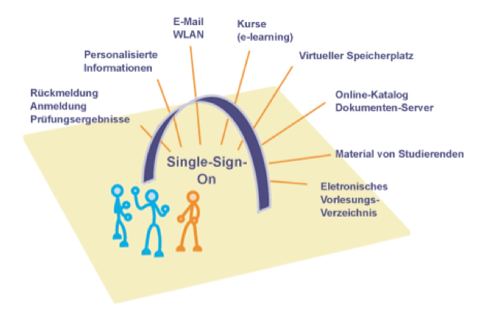
\includegraphics[width=10cm]{kapitel/gruppe1_2/bilder/SSO}
	\caption{Single-Sign-On\protect\footnotemark}
	\label{fig_sso}
\end{figure}\footnotetext{\cite[81]{deutsche_wissenschaft_2010}}


\subsubsection{IT Infrastructure Library (ITIL)}
\label{subsubsection_ITIL}
Zur Fokussierung der IT-Dienste auf Kundenorientierung und für eine stärkere Ausrichtung des 
IT-Bereichs an strategischen Organisationszielen, stehen Hochschulen und anderen Institutionen 
verschiedene Referenzmodelle zur Verfügung. Diese Modelle unterstützen bei der Bereitstellung klar 
definierter IT-Services, einer kennzahlengestützten Steuerung und Bewertung des IT-Managements und 
Umstrukturierung der IT-Organisation. Die IT Infrastructure Library (kurz ITIL) ist das international am 
meisten genutzte Referenzmodell. Es ist aus einer Sammlung von Beispielen guter Praxis entstanden 
und wird stetig weiterentwickelt. In ITIL werden sämtliche Prozesse in Beziehung zueinander gesetzt 
und definiert. Dazu gehören beispielsweise Konfigurationsmanagement, Kapazitäts-, Verfügbarkeits- 
und Finanzplanung, der Umgang mit Katastrophen, Störungs- und Problembehandlung, aber auch 
Service Level Vereinbarungen. ITIL ist durch seine Skalierbarkeit und Prozessorientierung auf 
Gesamtorganisationen, einzelne Abteilungen oder übergreifende Dienstleistungen anwendbar. Die 
Prozesse können unabhängig von einer konkreten IT-Infrastruktur genutzt werden, wodurch der 
Einsatz in vielen Bereichen ermöglicht wird. \footcite[Vgl.][34]{leitner_itil_2008}

\paragraph{Servicedesk}\mbox{}\\\\	

\label{subsubsection_service_desk}
Die Schaffung eines Servicedesks resultiert aus dem Verständnis, die Studierenden und Lehrenden als 
„Kunde“ zu betrachten, denen man serviceorientierte Dienstleistungen anbieten möchte. Zum anderen 
wird eine effizientere Ressourceneinsatzplanung im Verwaltungsbereich ermöglicht. Der Servicedesk ist 
die zentrale Anlaufstelle für jegliche Belange. Hier wird im Zuge des 1st Level Supportes eine Lösung 
der Anfrage ohne Kontaktierung weiteren Fachpersonals versucht. Zusätzlich stellt diese Ebene eine 
schnelle Reaktionszeit bei Störungen sicher. Sollte eine Sofortlösung nicht möglich sein, werden die 
Anfragen über ein Ticketsystem sortiert, priorisiert und den entsprechenden Bearbeitern zugeteilt. Hier 
wird die Bearbeitung zeitversetzt durch Spezialisten im 2nd Level Support fortgeführt. In der Abbildung 
\ref{fig_service_desk} ist der beschriebene Ablauf visualisiert, es handelt sich hier um die Infrastruktur 
der Universität Freiburg. \footcite[Vgl.][5]{klug_2008}

\begin{figure}[h!]
	\centering
	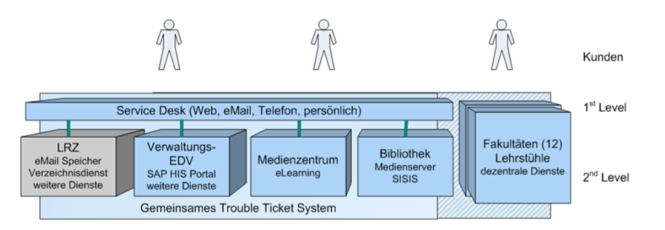
\includegraphics[width=\textwidth]{kapitel/gruppe1_2/bilder/ServiceDesk}
	\caption{Servicedesk: Beispiel an der Universität Freiburg\protect\footnotemark}
	\label{fig_service_desk}
\end{figure}\footnotetext{\cite[15]{bode_2007}}
\newpage

\paragraph{Change-Management}\mbox{}\\\\
Change-Management ist einer der ITIL-Prozesse und beschreibt wie auf Änderungsanfragen zu reagieren ist. Dabei durchläuft der Change (die Veränderung) nachfolgende feingranulare Aktivitäten:

\begin{enumerate}
	\item Change wird erfasst und klassifiziert
	\item Change wird bewertet und freigegeben
	\item Change wird bei Bedarf eskaliert
	\item Change wird implementiert
	\item Change wird getestet und abgenommen
	\item Change wird abgeschlossen
\end{enumerate}

Innerhalb dieses Prozesses gibt es die Rolle des Change Requestors, der die Anfrage stellt. Diese wird 
idealerweise an einer einzigen Stelle wie den Servicedesk aufgegeben, um sicherzustellen, dass alle 
Anforderungen vollständig erfasst und zentral gebündelt sind. Der Change Manager klassifiziert den 
Change und plant die Durchführung. Eine Beurteilung der Änderungsanfrage erfolgt anhand einer 
hochschulweiten vereinbarten Einstufung, die eine Klassifizierung nach Change-Typen vorsieht. In der 
Tabelle \ref{tab_typen_von_changes} sind hier die Change-Typen \glqq Normal Change\grqq, \glqq 
Security Change\grqq und \glqq Notfall Change\grqq als Beispiel aufgeführt, wobei nur im Notfall eine 
Freigabe durch den Change Manager notwendig ist. Der Change Builder setzt die Veränderung 
letztendlich um und der Change Approver prüft und testet die Änderung. 
\footcite[Vgl.][48]{breiter_implementierung_2011}

\begin{table}[h!]
	\begin{tabularx}{\textwidth}{|X|X|X|}
		% Überschriften
		\hline \textbf{Change-Typ} & \textbf{Beschreibung} & \textbf{Genehmigung}\\
		% Zeile 1
		\hline Normal Change & Normalfall & keine Genehmigung durch den Change Manager\\ 
		% Zeile 2
		\hline Security Change & Änderungen für einen bestimmten Anwenderkreis & keine Genehmigung 			durch den Change Manager\\
		% Zeile 3
		\hline Notfall Change & Sofortige Freigabe und Bearbeitung & Genehmigung durch Change 				Manager nötig\\
		\hline
	\end{tabularx}
	\caption{Typen von Changes\protect \footnotemark}
	\label{tab_typen_von_changes}
\end{table}\footnotetext{\cite[48]{breiter_implementierung_2011}}

\paragraph{Service Level Agreements}\mbox{}\\\\
„Service Level Agreements“ (SLAs) sind verbindliche Vereinbarungen zwischen dem Leistungsempfänger 
und dem Leistungserbringer. Die SLAs sichern die Bereitstellung von IT-Dienstleistungen, regeln die 
Dienstleistungsqualität und definieren die Preise für die Erbringung von Leistungen. Weiter werden auch 
Reaktionszeiten je nach Schweregrad definiert und Konventionalstrafen für den Fall von einer 
Überschreitung festgelegt. Betriebszeiten und Ausfallsicherheit wichtiger Infrastruktur sind ebenfalls 
Bestandteile solch einer Vereinbarung.
Zusammengefasst sind SLAs für Dienstleistungsempfänger ein wichtiges Instrument zur Sicherheit und 
Kenntnisnahme über den Leistungsumfang, die Leistungskosten, die minimale Leistungserbringung 
und der benötigten Reaktionszeit. Informationsmanager nehmen hierbei eine beratende Rolle ein und 
unterbreiten zusätzlich Vorschläge zur fachlichen Beschreibung von Zielvorgaben. 
\footcite[Vgl.][499]{heinrich_stelzer_2011}


\subsubsection{Chief-Information Officer (CIO)}
\label{subsubsection_cio}
Der Chief Information Officer (CIO) ist die Berufsbezeichnung für eine Person/Führungskraft, die 
verantwortlich für die Informationstechnik und Anwendungen einer Hochschule ist. 
\footcite[Vgl.][]{beuschel_2009}

\paragraph{Aufgaben und Funktionen des Informationsmanagers}\mbox{}\\\\
\label{aufgaben_funktionen_informationsmanager}
Die Aufgaben des CIO bestehen in der Entwicklung einer IT-Infrastruktur-Strategie und der Ausrichtung der IT auf die Unternehmensstrategie. Seine Tätigkeiten lassen sich im operativen Geschäft auf 3 Kernaufgaben festlegen: 
\begin{enumerate}
	\item Das Planen und Implementieren von Software- und Hardware-Architekturen 
	\item Priorisierung neuer Steuerungsprozessen, sowie neuer Anwendungen
	\item Bereichsübergreifende Koordination
\end{enumerate}

Im Rahmen des Plan-Do-Check-Act-Zyklusses (PDCA), der im Kapitel  \ref{subsubsection_kontinuierlicher_verbesserungsprozess} näher erläutert wird,  sollte er strategische Vorschläge unterbreiten, wie Informationen zur Zielerreichung und Gewinnmaximierung innerhalb der Hochschule eingesetzt werden können. Außerdem hat er Informationen auf die Hochschulkultur und –praxis  abzustimmen und unter Berücksichtigung all dieser Aspekte individuell passende und benutzerfreundliche Werkzeuge auszuwählen. In seiner Verantwortung steht, dass erfolgsentscheidendes Wissen auch in schwierigen Situationen und bei hoher Fluktuation in der Hochschule erhalten bleibt. Organisationen, die über einen CIO mit solch einem Aufgabenprofil verfügen, sind selten. Sie sind eher in modernen Großkonzernen oder Unternehmen mit einer besonderen Affinität zu internetgestützter Kommunikation vorzufinden. \footcite[Vgl.][404]{becker_gora_uhrig_2012}

Aus dieser Aussage lässt sich für deutsche Hochschulen ableiten, dass der Einsatz eines CIOs gut überlegt sein muss. Kleine Hochschulen besitzen einen geringeren Kommunikationsbedarf, als große Hochschulen. Daher ist der Nutzen eines CIOs im Vorfeld gut zu prüfen. Das Kapitel \ref{section_einsatz_cio} wägt den Einsatz eines CIOs für die Hochschule Emden/Leer ab.

\paragraph{Anforderungsprofil}\mbox{}\\\\
\label{anforderungsprofil_informationsmanager}
Ein gutes Anforderungsprofil eines CIOs umfasst eine Mischung aus technischem Wissen, unternehmerischer Denkensweise und Managementfähigkeiten. Für die erfolgreiche Arbeit sind konzeptionelle und analytische Befähigungen aber auch Schlüsselqualifikationen wie Entscheidungsstärke, Organisationstalent, Teamfähigkeit, Führungsqualifikation, Kontaktfähigkeit, Kenntnisse im Projektmanagement und  in der strategischer Planung wichtig. In Abbildung \ref{efec} sind außerdem persönliche Merkmale wie Sensibilisierung und soziales Kompetenzwissen als Erfolgsfaktoren für einen CIO aufgeführt. Die Beziehungen zum CEO und ein Aufbau einer gemeinsamen Vision sind ausschlagegebend für die erfolgreiche Arbeit. Entscheidend ist auch das glaubwürdige Auftreten innerhalb der Hochschule.\footcite[Vgl.][150]{krcmar_einfuhrung_2015}

\begin{figure}[h!]
	\centering
	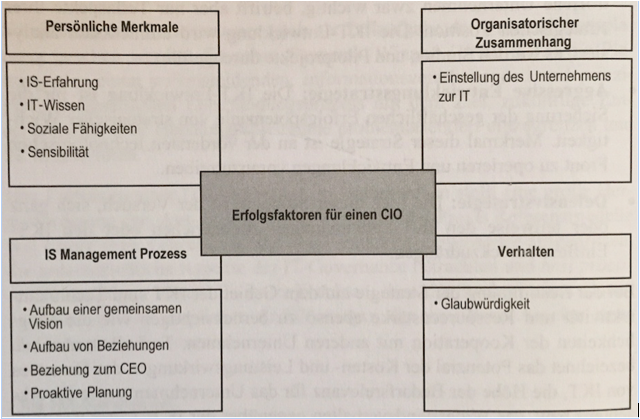
\includegraphics[width=15cm]{kapitel/gruppe1_2/bilder/erfolgsfaktoren_cio} 
	\caption{Erfolgsfaktoren für einen CIO\protect\footnotemark}
	\label{efec}
\end{figure}\footnotetext{\cite[150]{krcmar_einfuhrung_2015}}

\paragraph{Eingliederung in die Hochschulhierarchie}\mbox{}\\\\
Nachdem die grundsätzlichen Aufgaben eines Informationsmanagers erläutert wurden, ist noch die Ansiedlung dieses Postens innerhalb der Hochschulhierarchie zu klären. Das Spektrum reicht hier vom CIO mit Leitungsfunktion repräsentiert durch einen Vizepräsident bis hin zu einer kollektiven Teilung innerhalb des Lenkungsausschusses durch mehrere Personen. Im Detail wird hierauf in Kapitel \ref{subsubsection_zki} eingegangen, insgesamt werden 4 verschiedene Umsetzungstypen unterschieden. \footcite[Vgl.][10]{leitner_itil_2008}

\subsection{Prozessorientierung}
\label{subsection_prozessorientierung}
Die Prozessorientierung ist ein grundlegendes Konzept des Geschäftsprozessmanagements, worunter 
die Gestaltung, Ausführung und Beurteilung von Prozessen verstanden wird. Ein Prozess ist eine 
zusammenhängende Abfolge von Einzelfunktionen, zwischen denen logische Verbindungen bestehen, 
wie in Abbildung \ref{fig_aufgaben_vs_prozess} mit Pfeilen visualisiert wurde. 
\footcite[Vgl.][60]{krcmar_einfuhrung_2015} Weiter lässt sich aus der Abbildung anhand des 
Organigramms ablesen, dass die Gliederung der IT-Organisation an Hochschulen oft funktional 
aufgestellt ist, konkret zu erkennen an dem Netzwerk- und Systembetrieb, Nutzersupport (Servicedesk) 
oder dem Anwendungsmanagement. Diese Aufgabenorientierung erlaubt eine stärkere Spezialisierung 
in den jeweiligen Fachgebieten der Mitarbeiterinnen und Mitarbeiter, widerspricht aber dem Gedanken 
einer Prozessorientierung. Hier ist daher eine klare Definitionsabgrenzung durchzuführen, denn das 
Handeln in Prozessen erfordert eine Abkehr von aufgabenorientierten Verfahrensweisen. 
Prozessorientiert zu denken bedeutet, sich nicht nur auf eine Aufgabe zu konzentrieren, sondern den 
Gesamtkontext zu betrachten, sprich das Zusammenspiel und die Wechselwirkungen zwischen allen 
Einzelfunktionen eines Prozesses. Erst durch die Betrachtung der Verkettung einzelner Aufgaben 
werden nämlich komplexe und betriebswirtschaftliche Prozesse ersichtlich. 
\footcite[Vgl.][274]{heinrich_stelzer_2011}

\begin{figure}[h!]
	\centering
	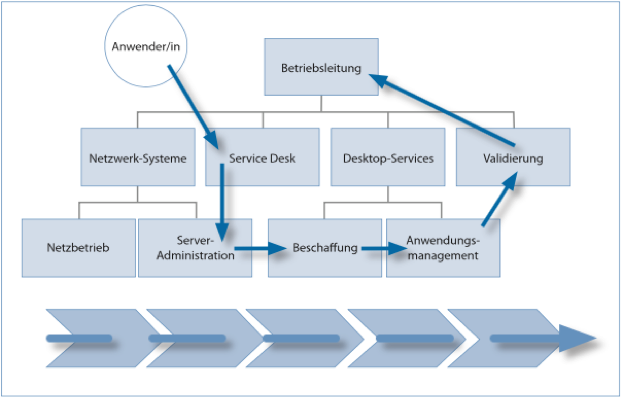
\includegraphics[width=15cm]{kapitel/gruppe1_2/bilder/aufgaben-versus_prozessorientierung} 
	\caption{Aufgaben- versus Prozessorientierung\protect\footnotemark}
	\label{fig_aufgaben_vs_prozess}
\end{figure}\footnotetext{\cite[Vgl.][35]{leitner_itil_2008}}

Die Erreichung der Prozessorientierung kann auf unterschiedliche Weise erfolgen, zum Beispiel durch 
eine kontinuierliche Prozessverbesserung oder die Gestaltung und Anpassung von IT-Strukturen 
\footcite[Vgl.][45]{wissensmanagement_2010}. Im Rahmen des Kapitels 
\ref{subsubsection_kontinuierlicher_verbesserungsprozess}  wird der in der oberen Abbildung gezeigte 
kontinuierlicher Verbesserungsprozess beschrieben, evaluiert und letztendlich optimiert.

\subsubsection{Kontinuierlicher Verbesserungsprozess}
\label{subsubsection_kontinuierlicher_verbesserungsprozess}
Das Ziel des kontinuierlichen Verbesserungsprozesses ist die stetige Verbesserung von Zuständen in 
kleinen Schritten und die Wahrung der  Zustandsverbesserung, wie in Abbildung 
\ref{fig_kontinuierliche_verbesserung} gut veranschaulicht. Zur Umsetzung systematischer 
Verbesserungsmaßnahmen, wird ein in 4. Phasen aufgeteilter Regelkreis angewandt.

\begin{figure}[h!]
	\centering
	
\includegraphics[width=5cm]{kapitel/gruppe1_2/bilder/kontinuierlicher_verbesserungsprozess} 
	\caption{Kontinuierlicher Verbesserungsprozess\protect\footnotemark}
	\label{fig_kontinuierliche_verbesserung}
\end{figure}\footnotetext{\cite{yasar_kvp_2015}}

In der Phase Plan wird sich die Frage gestellt, was und wie etwas zu tun ist. Auf die Prozessorientierung angewandt, lässt sich hier auf die Prozessdefinition und –analyse schließen. Die Phase Do beschäftigt sich mit der Frage was erreicht wurde und steht für die Ausführung, also sinnbildlich für die Prozesskonstruktion. Bei der Check-Phase geht man auf die Frage ein, was noch zu tun ist und ob die Aufgaben nach Plan erfüllt sind, ableitbar auf eine Prozessvalidierung. In der letzten Phase Act wird überprüft, welche Dinge verbessert werden können, das für eine Prozessoptimierung und –automatisierung spricht.\footcite[Vgl.]{yasar_kvp_2015}

\paragraph{Prozessidentifizierung und -analyse}\mbox{}\\\\
\label{paragraph_prozessidenifizierung}
Die Aufgabe der Prozessidentifizierung ist es, Prozesse zu bestimmen und zu beschreiben, die mit hoher Priorität geplant, gesteuert und verbessert werden sollen. In der Prozessanalyse werden dann die einzelnen Elemente eines Prozesses und deren Beziehung untereinander bestimmt und beschrieben. \footcite[Vgl.][276]{heinrich_stelzer_2011}
Angewandt auf den Prozess in der Abbildung \ref{fig_aufgaben_vs_prozess} des Kapitel \ref{subsection_prozessorientierung} kann folgendes abgeleitet werden:
Der Anwender meldet eine Störung innerhalb einer Fachapplikation wie zum Beispiel der Studierendenverwaltung dem Servicedesk der Hochschule. Dieser analysiert, beschreibt und priorisiert den eingehenden Fall. Innerhalb des First-Level-Supportes und bestehender Fehlerprotokolle/-dokumentationen wird versucht, eine Sofortlösung zu erzielen. Ist dies nicht erfolgsversprechend, wird bei einer fehlerhaften Serverkonfiguration der Server-Administrator verständigt. Dieser entdeckt bei seiner Untersuchung ein fehlendes Update der Fachapplikation und beauftragt damit die Beschaffungsabteilung. Das Einspielen des Updates wird durch das Anwendungsmanagement auf einem Testsystem durchgeführt, die sich anschließend zwecks Qualitätssicherung mit der Testgruppe zur Validierung abstimmt. Nach Freigabe durch die Betriebsleitung kann die Aktualisierung auf dem Produktivsystem eingespielt werden.
Ein in der Abbildung nicht aufgeführter möglicher Rückweg wäre: Nach Freigabe des Updates wird durch das Anwendungsmanagement die Installation auf dem Produktivsystem veranlasst. Der Servicedesk wird hierrüber nach erfolgreichem Abschluss informiert, der die Fehlerbehandlung protokolliert und den Endanwender über die Lösung der gemeldeten Störung unterrichtet.

\paragraph{Prozesskonstruktion und –sichtbarkeit}\mbox{}\\\\
\label{paragraph_prozesskonstruktion_und_sichtbarkeit}
Um die im vorherigen Kapitel bei der Prozessanalysendefinition erwähnten Elemente sichtbar zu machen, werden Prozessketten verwendet. Diese eigenen sich, um den Ablauf bestehender Prozesse und die Beziehung der einzelnen Elemente untereinander zu visualisieren. Aber nicht nur der Ist-Prozess, sondern auch der Soll-Prozess kann mittels Prozessketten modelliert werden. Zur Verfügung stehen unterschiedliche Modellierungselemente, beispielsweise ein Rechteck zur Symbolisierung einer Funktion, eine Ellipse als organisatorisches Element (Prozessstart, Prozessende) oder Pfeile, die einen Informationsfluss veranschaulichen. \footcite[Vgl.][64]{krcmar_einfuhrung_2015} Zur Steigerung der Prozesseffizienz wurden in Kapitel \ref{subsubsection_prozessoptimierung_durch_minierung_der_durchlaufzeiten} unterschiedliche Durchlaufoptimierungen aufgeführt: \glqq Weglassen\grqq, \glqq Auslagern\grqq, \glqq Zusammen fassen\grqq, \glqq Parallelisieren\grqq, \glqq Verlagern\grqq, \glqq Beschleunigen\grqq, \glqq Keine Schleifen\grqq und \glqq Ergänzen\grqq.

Im Sinne des kontinuierlichen Verbesserungsprozesses und der in diesem Kapitel verwiesenen Prozesskonstruktion wurde im Anhang in der Abbildung \ref{fig_prozessoptimierung_gesamt} der im Kapitel \ref{paragraph_prozessidenifizierung} beschriebene Prozess der Fehlerbehandlung einer Fachapplikation mittels Prozesskette abgebildet. In der Zeilenbeschreibung sind die Zuständigen der jeweiligen Aufgaben aufgeführt. Der Prozess startet in der ersten Zeile bei „Start“ und ist der vorgegebenen Pfeilrichtung entsprechend zu lesen bis hin zum Prozessende.

\paragraph{Prozessevaluierung}\mbox{}\\\\
„Der wesentliche Zweck der Prozessevaluierung besteht darin, zu überprüfen, ob ein Geschäftsprozess gemäß den Vorgaben ausgeführt wird. Relevante Vorgaben können in Prozessentwürfen, Verfahrensanweisungen und Arbeitsanleitungen beschrieben sein“. \footcite[277]{heinrich_stelzer_2011} Es wird sich die Frage gestellt, ob die Prozesse so ausgeführt werden, wie sie in den Prozessmodellen beschrieben wurden und ob der Geschäftsprozess der kontinuierlichen Verbesserung unterliegt. \footcite[Vgl.][277]{heinrich_stelzer_2011} In unserem Beispiel wurde die Prozessmodellierung auf Basis der Prozessbeschreibung erstellt, wodurch die Prozessevaluierung positiv abschließt. Diese Evaluierung muss natürlich in regelmäßigen Abständen wiederholt werden, um zu überprüfen, ob der Gesamtprozess noch nach Plan läuft. Trotz positiver Bewertung kann auch unser Beispielprozess von einer Prozessoptimierung profitieren.

\paragraph{Prozessoptimierung}\mbox{}\\\\
\label{paragraph_prozessoptimierung}
Die Prozessoptimierung bezeichnet alle Maßnahmen zur Veränderung von Prozessen, um die Kosten zu senken, Durchlaufzeiten zu verkürzen, Innovationsfähigkeit zu erhöhen oder die Qualität zu steigern. \footcite[Vgl.][280]{heinrich_stelzer_2011}
Die im Kapitel \ref{paragraph_prozesskonstruktion_und_sichtbarkeit} gewonnenen Erkenntnisse zur Steigerung der Prozesseffizienz wurden auf unseren Fall angewandt und mündeten in einer optimierten Prozesskette. Dieses Kapitel konzentriert sich aufgrund der Komplexität auf den ersten Teilprozess, sprich die Meldung des Fehlers bis zur Freigabe des Updates. Der Rückweg in Form der Installation auf dem Produktivsystem und der Erfolgsmeldung an den Kunden ist der Vollständigkeit halber im Anhang in Abbildung \ref{fig_prozessoptimierung_gesamt} mit aufgeführt, ist aber nicht Bestandteil dieser Ausarbeitung.
Die erste Spalte der Abbildung \ref{fig_prozessoptimierung} zeichnet den aktuellen Ist-Zustand auf. Das Ergebnis einer Prozessoptimierung ist in der zweiten Spalte erkennbar, auf das nachfolgend weiter eingegangen wird. Damit die Innovation Einzug in der Hochschule hält, wäre eine übergreifende Service- und Programmüberwachung denkbar. Sie ermöglicht das entdecken und identifizieren von Fehlern vor der Meldung durch einen Endanwender. Parallel dazu wird ein Automatismus geschaffen, der neue Updates für alle Fachapplikationen sucht und bei Entdeckung an die übergreifende Überwachungssoftware meldet. Wird ein neues Update festgestellt, wird der Server-Administrator informiert, um die Serverkonfiguration zu prüfen. Es ist sinnvoll, seine Kompetenzen um das Einspielen von Updates für Applikationen zu erweitern. Nur spezifische Störungen innerhalb der Anwendung oder konkrete Nachfragen zur Bedienung sollten an das Anwendungsmanagement weitergeleitet werden.  Die Testgruppe prüft anhand vordefinierter Testfälle die Funktionsfähigkeit der Anwendung. Der Betriebsleiter gibt das Update nach positivem Testfeedback frei.
Um die einzelnen Maßnahmen zur Prozessoptimierung aufzugreifen, sind im Schaubild Kreise mit Zahlen aufgeführt:

\begin{enumerate}
	\item Maßnahme Weglassen: Im Optimalfall wird der Endanwender von einer Störung nichts mitbekommen
	\item Maßnahme Parallelisierung: Das Laden von Updates wird automatisiert und findet parallel zur Programmüberwachung statt. So wird eine verkürzte Durchlaufzeit erzielt, da der Server-Administrator sofort informiert und auf bereits heruntergeladene Updates zugreifen kann.
	\item Maßnahme Ergänzen: Durch die Einführung einer übergreifenden Überwachungssoftware wird ein neuer Teilprozess ergänzt.
	\item Maßnahme Zusammenführen: Der Serveradministrator prüft nicht nur Serverkonfigurationen, sondern spielt auch Updates ein
	\item Maßnahme Auslagern: Die Fachabteilung Beschaffung muss die Updates nicht mehr selbst herunterladen, ein Automatismus auf einem Server übernimmt diese Tätigkeit.
\end{enumerate}


\begin{figure}[h]
	\centering
	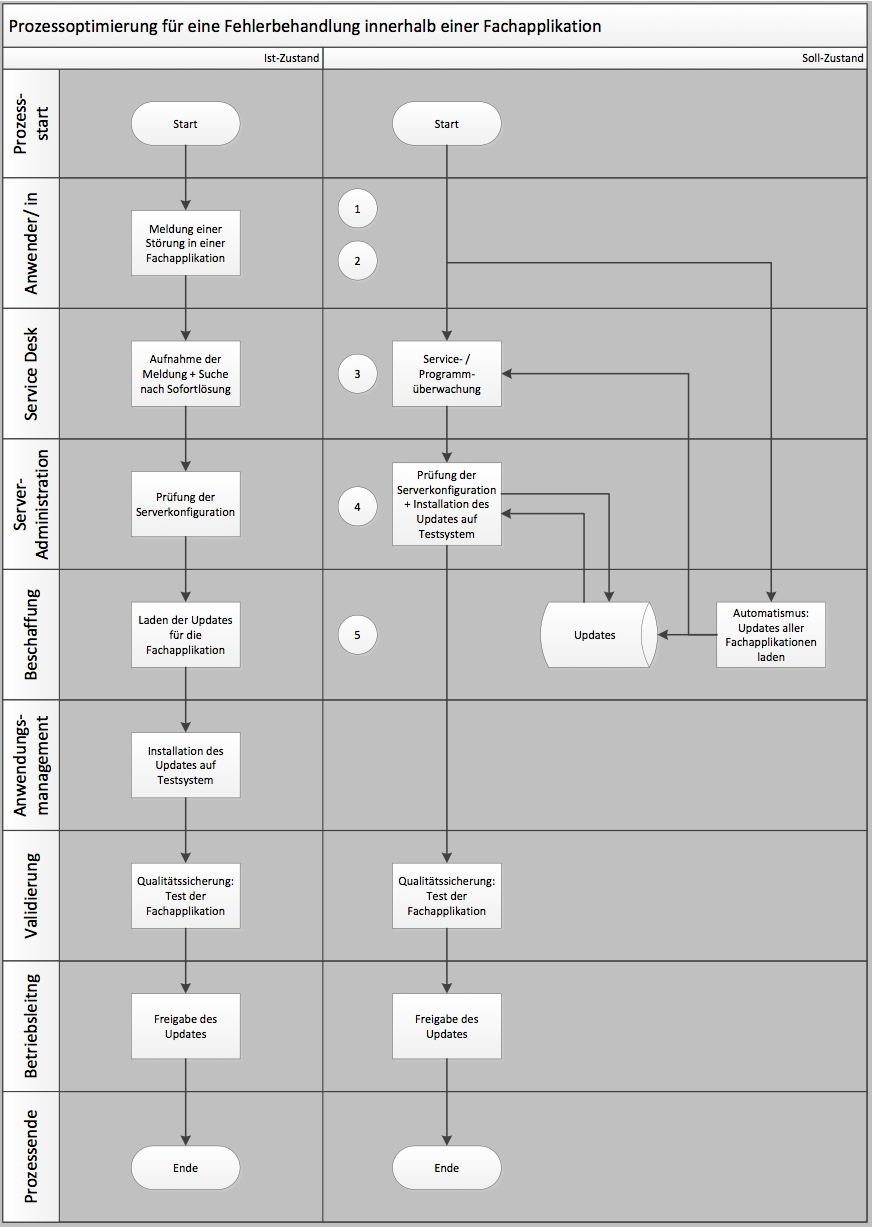
\includegraphics[width=\textwidth]{kapitel/gruppe1_2/bilder/prozessoptimierung} 
	\caption{Prozessoptimierung für eine Fehlerbehandlung}
	\label{fig_prozessoptimierung}
\end{figure}
\clearpage

\subsubsection{Gestaltung und Anpassung von IT-Strukturen}
\label{subsubsection_gestaltung_IT_strukturen}
Die Gestaltung und Anpassung von IT-Strukturen ist zur Prozessoptimierung durch Zentralisierung, Standardisierung und Outsourcing erreichbar. Wie diese Gestaltungsmaßnahmen bereits in bestehenden deutschen Hochschulen zum Einsatz kamen, erläutert Kapitel \ref{section_umsetzung_der_trends_in_den_betrachteten_hochschulen}.


\paragraph{Zentralisierung}\mbox{}\\\\
\label{paragraph_zentralisierung}
Im Hochschulbereich haben sich einige Lehrstühle und Institute ihre eigene IT-Abteilung geschaffen. Dies gilt beispielsweise für viele Leiter von Forschungsprojekten, für die Verwaltung und die Bibliothek, die eigene IT-Dienstleistungen erbringen. Das hohe Maß an Dezentralisierung der IT-Betriebsorganisationen führt zu einer Redundanz der IT-Service-Erbringung. Es ließe sich ein Parallelaufbau von betriebsrelevanter Infrastruktur wie Netz- und Stromversorgung, Belüftung und Klimatisierung vermeiden.
\footcite[Vgl.][22]{stratmann_it_2013}. Auch das doppelte Bereitstellen von beispielsweise Mailservices oder Groupware ist nicht sinnvoll. Des Weiteren wird mit diesen Standard-IT-Dienstleistungen mehrfach Personal gebunden, das mit der zunehmenden Komplexität der Basisdienstleistungen oft überfordert ist. 
Die Institute können sich nicht selbst auf allen Ebenen mit hochwertiger IT-Dienst-Betreuung befassen. Die vielen Insellösungen sind zusätzlich unwirtschaftlich und für eine hochschulweite Integration des Informationsmanagements oft hinderlich. Die Institute müssen Strategien entwickeln, um gemeinsame Synergieeffekte zu nutzen und die begrenzten IT-Betreuungsressourcen sinnvoll einzusetzen.
Die Zentralisierung von Diensten ermöglicht eine einfach zu koordinierende Beschaffung von Hard- und Software. Alle Systeme sind durch die zentrale Planung und Einbettung gut aufeinander abgestimmt und ergeben größere Ausfallsicherheit mit hoher Verfügbarkeit. Das stärkt die Stabilität und Robustheit des IT-Gesamtsystems. Die Redundanz in dem Personaleinsatz und der Serviceerbringung entfällt. \footcite[Vgl.][22]{moenkediek_2006}


\paragraph{Standardisierung}\mbox{}\\\\
\label{paragraph_standardisierung}
Unter der Standardisierung in Hochschulen wird die einheitliche Nutzung von Basisdiensten und Grundfunktionalitäten verstanden. Konkret soll die Vereinheitlichung von Anwendungsprogrammen, Prüfungsordnungen und IT-Infrastrukturen in den Fachbereichen erzielt werden. Über ein Softwareverteilungstool kann eine gleiche Version aller Applikationen sichergestellt werden. Zur Realisierung von einheitlicher IT-Infrastruktur wäre eine Zentralisierung der Serviceleistungen denkbar, wie im vorherigen Kapitel beschrieben. Die Einführung von ITIL-Standardprozessen wäre ein möglicher Weg der Umsetzung und mittels SLAs könnten auch die Reaktionszeiten auf Fehlermeldungen festgelegt werden. Ein Informationsmanager (siehe Kapitel \ref{subsubsection_cio}) würde für eine kontinuierliche Einführung und Einhaltung der Standards in allen Fachbereichen Sorge tragen. Eine Zertifizierung nach standardisierten Normen (ISO 200000), wird in den kommenden Jahren ebenfalls an Bedeutung gewinnen.\footcite[Vgl.][168]{breiter_implementierung_2011}


\paragraph{Outsourcing}\mbox{}\\\\
\label{paragraph_outsourcing}
Outsourcing besteht aus den Wörtern \glqq Outside\grqq{}, \glqq Ressource\grqq{} und \glqq Using\grqq{}. Gemeint ist damit, dass einzelne Aufgaben der IT, wie bspw. Infrastruktur, Applikationen, Prozesse, Personal oder gesamte IT-Aufgaben, auf Basis einer vertraglichen Vereinbarung, für einen definierten Zeitraum an einen externen Anbieter ausgelagert werden.\footcite[Vgl.][164]{krcmar_einfuhrung_2015} Konkrete Beispiele im Bereich der Informationstechnologie für Hochschulen wären der Betrieb des Rechenzentrums, der Anwendungsentwicklung oder der Telekommunikationsnetzwerke an andere Unternehmen abzugeben. Der Informationsmanager verspricht sich einen besseren Zugriff auf notwendige Ressourcen, Verlagerung möglicher Risiken und transparentere Ausgaben durch eine Kooperation mit Outsourcing-Gebern. Dagegen stehen erhöhter Koordinationsaufwand, komplizierte Vertragsgestaltungen und räumliche / zeitliche Distanz und damit fehlendes Vertrauen in den neuen Kooperationspartner.\footcite[Vgl.][195 ff.]{barthelemy_2001}

\subsection{Konklusion Serviceorientierung und Prozessorientierung}
Schlussfolgend aus der Definition der Serviceorientierung und der Prozessorientierung lässt sich ableiten, dass sich beide Orientierungen nicht ausschließen, sondern ergänzen.  Dienstleistungsorientierung bedeutet, dass die Bereitstellung von Informationssystemen als Leistung und Dienst am Kunden selbst verstanden und gesteuert wird. Genau dies ergänzt die Prozessorientierung mit optimierten Prozessen zur Erbringung dieser Leistungen. 
Die Hochschule Emden/Leer setzt beide Orientierungen ein, möchte sich aber laut dem Hochschulrechenzentrumsleiter Günter Müller in Richtung Prozessorientierung weiterentwickeln. \footcite{gunter_muller_interview} So empfiehlt es sich auf eine effektive und effiziente Gestaltung der Dienstleistungen zu konzentrieren und durch Standardisierung einheitliche Prozesse zu schaffen.
\section{Neue Medien - AH}

Im folgenden Abschnitt werden Hochschultrends im Bereich der „Neuen Medien“ beschrieben. Dabei wird auf das fortschreitende Verlangen nach „Consumerization“, der Wandel zur heterogenen Nutzung der Angebote über verschiedenartige Geräte, der gleichzeitig stattfindende Wunsch zur Zentralisierung der Administration und Infrastruktur und der Imagebildung über das Marketing mit Hilfe unter anderem des Onlineauftritts, der Kommunikation in sozialen Medien und der App-Informationssysteme eingegangen. Die genannten Trends werden nur grob aufgezeigt und in Folgekapiteln aufgegriffen und auf die Hochschule Emden/Leer angewendet.


% ---------------------------------------
\subsection{Infrastruktur und Management}
Die Infrastruktur und das Management an Hochschulen befinden sich seit der Digitalisierung in einem ständigen Wandel. Neue Technologien führen immer wieder zu neuen Begehrlichkeiten, wie z.B. Standardisierung, Zentralisierung oder Prozessorientierung. Im folgenden Abschnitt werden die aktuellen Trends an einigen wichtigen Aspekten betrachtet.


\subsubsection{Netzinfrastruktur, Consumerization und BYOD}
\label{netzinfrastruktur_consumerization_und_byod}
Im Zuge der Consumerization haben sich die Grenzen der Nutzung von privater und beruflicher Software und Geräte aufgelöst. Zum einen bringen Benutzer Software und Hardware mit, die Sie im beruflichen Umfeld verwenden möchten, aber auch umgekehrt, wollen Benutzer beruflich genutzte Software privat nutzen. Eine homogen gestaltete Infrastruktur ist damit hinfällig geworden, in dem Sinne, dass nicht mehr per Vorgabe geregelt wird, eine bestimmte Software- und Hardwarevariante zu verwenden.

Der Trend zum Bring Your Own Device (BYOD) hat veranlasst, dass eine Infrastruktur flexibel 
gestaltet wird. Insbesondere auch die gestiegene Nutzung von Mobilgeräten wie Smartphones 
und Tablets hat dazu geführt, dass Software neuen Vorgaben gerecht werden muss. Gegenüber 
der Steigerung der Produktivität müssen jedoch die Kosten im Auge behalten werden. Im 
Hinblick auf die Implementierung sind dabei Aspekte wie Sicherheit und Infrastruktur zu 
berücksichtigen.\footcite{forrester_research_2012}

Viele Hochschulen in Europa haben sich mittlerweile dem Projekt eduroam (education roaming) angeschlossen. Eduroam ist eine Netzinfrastruktur und ermöglicht die Nutzung von WLAN und LAN an jeder teilnehmenden Hochschule durch vorherige Authentifizierung mit einem Hochschulaccount und einem beliebigen Gerät.
Eduroam als standardisierte Lösung macht die Teilnahme verschiedener Geräte und Standorte im Zuge von BYOD sehr einfach. Geringere Support-Aufwendungen auf der anderen Seite ermöglichen es die Serviceorientierung teilweise abzulösen und durch Prozessorientierung zu ersetzen. Der Aufwand erhöht sich jedoch für die Administratoren durch „die Offenheit der Gerätewahl.“\footcite{wickhill_byod_2013} Der Sicherheitsaspekt spielt daher eine große Rolle. An den Standorten selber kommt es in Folge der Offenheit für die Benutzer wiederum so zur Steigerung der Produktivität und Benutzerzufriedenheit, weil die Arbeitsabläufe flüssiger und effizienter werden.

\subsubsection{Software für Forschung und Lehre}
\label{software_forschung_lehre}
Software- und Service-Anbieter bieten häufig spezielle Angebote für Hochschulangehörige. Eines der bekanntesten ist dabei Dreamspark. Das Netzwerk Dreamspark ermöglicht es Studenten und Bediensteten im Rahmen von Forschung und Lehre kostenlos eine Vielzahl von Microsoft Softwareprodukten zu erhalten und auf Ihren Geräten zu installieren.

Viele Hochschulen, unter anderem die Hochschule Osnabrück, Hochschule Hannover oder auch die Hochschule Emden/Leer ermöglichen die Teilnahme am Dreamspark-Netzwerk.

Neben Dreamspark bieten Hochschulen über Ihre Website Links und Hinweise zu weiteren Angeboten, siehe unter anderem. TH Nürnberg.\footcite{thnuernberg_software_2015} Die zentrale Anlaufstelle für Hochschulangehörige ermöglicht die schnelle Auffindbarkeit und Erkundung in Frage kommender Software, wie zum Beispiel folgender Angebote:

\begin{itemize}
	\item GitHub \footcite{github_edu}
	\item JetBrain \footcite{jetbrains_edu}
	\item Video2Brain \footcite{video2brain_edu}
\end{itemize}


\subsubsection{Identitätsmanagement}
\label{subsubsection_identitatsmanagement}
Ein umfassendes Identitätsmanagement setzt eine komplexe Architektur voraus. Die zwei Hauptfunktionen des Identitätsmanagement klassifiziert sich in:

\begin{itemize}
	\item neue Benutzer anlegen
	\item Benutzer entfernen
\end{itemize}

Die Hochschulen gehen die Entwicklung der Zentralisierung vgl. hierzu Kapitel 
\ref{paragraph_zentralisierung}. Dabei soll die Einrichtung und Löschung der Benutzer-Daten schnell, klar 
und nachvollziehbar hinterlegt werden 
können.\footcite{harnisch_identitat_2008}

Dem Benutzer wird der Zugriff auf die Dienste der Hochschule soweit wie möglich erleichtert, hier wird vor allem auf die Einmalanmeldung (Single-Sign-On) gesetzt. Dem Benutzer werden alle angeschlossenen Dienste der Hochschulen zugänglich gemacht, ohne sich mehrfach Authentifizieren zu müssen. Unter anderem wird dabei auf Shibboleth gesetzt, vgl. Kapitel \ref{shibboleth_sso}.


\subsubsection{E-Mail}
Ein integraler Bestandteil an Hochschulen ist die E-Mail Infrastruktur. Der Trend geht zu einem zentral-administrierbaren System. Im Sinne des Consumerization wird die Nutzung des E-Mail Services offen gestaltet für alle vorstellbaren Endgeräte und Programme. Die zentralen Systeme gewähren die heterogene Nutzung über Desktop, Mobilgeräte und Webmailer. \footcite{hszwickau_zahlen_2015}


\subsubsection{E-Learning Plattform}
\label{subsubsection_e_learning_plattformen}
Das elektronische Lernen setzt auf den Einsatz digitaler Medien. Das Blended Learning vereint das Präsenzstudium mit dem E-Learning und hat dabei drei substantiell wichtige Lerndomänen

\begin{itemize}
	\item das lernen online durch Kommunikation
	\item distanziert ohne Interaktion
	\item und in der Präsenz.
\end{itemize}

Auch im Präsenzstudium wird zunehmend nicht nur auf offline Medien Skripte oder Bibliothek gesetzt, sondern zusätzlich auf Aufzeichnungen, Videochats, online Einsendeabgaben und Foren.

An Hochschulen wird zum gr\"oßten Teil auf eine der zwei größeren Plattformen gesetzt.\footcite{oevel_lange_2008}

\begin{itemize}
	\item Moodle www.moodle.com
	\item ILIAS www.ilias.de
\end{itemize}

Die Plattformen waren ursprünglich für das Onlinestudium gedacht, ziehen jedoch mehr und mehr in das Präsenzstudium ein. Dabei wird das Potential der Plattform noch selten ausgereizt und ist nicht verpflichtend. Sie erweitern das Präsenzstudium aber um zusätzliche Möglichkeiten.
Neben dem Platzhirsch wie Moodle vgl. Kapitel \ref{paragraph_moodle} werden noch weitere Systeme wie Lon-Capa und StudIP eingesetzt.

Die Plattformen ermöglichen es, dass Skripte zur Verfügung gestellt und kontinuierlich weiterentwickelt werden können. Dabei ist auch die Kooperation mehrerer Autoren und Outsourcing möglich, vgl. auch Kapitel \ref{paragraph_outsourcing}. Um diese Skripte entsteht dann ein Ökosystem aus Übungsaufgaben, Videos und Forenbeiträgen.



% ---------------------------------------
\subsection{Dokumentenverwaltung}
\label{dokumentenverwaltungssysteme}
Im Abschnitt Dokumentenverwaltung wird auf die an Hochschulen eingesetzten Software-Trends und auf das Druckzentrum der Uni Münster eingegangen.


\subsubsection{Wiki}
Das Wiki ist ein Dienst zur Erfassung ungeordneter, miteinander verknüpfbarer Texte. Sie sind sehr flexibel einsetzbar und werden daher von sehr vielen Hochschulen eingesetzt. Es lassen sich schnell Informationen versionsbasiert gemeinsam zusammentragen und verwalten.\footcite[Vgl.][65]{schmidtjh_2013}

Wikis stellen oft die erste Basis für Informationsverwaltungen, aus denen konzentriertere Informationssysteme entstehen können in Form von Websites oder auch FAQs, Anleitungen und vieles mehr.


\subsubsection{Clouds und Big Data}
Clouds ermöglichen den einfachen Datenaustausch großer Dateien mit verschiedenen Zugriffsrechten. Eingeteilt werden können die Clouds in

\begin{itemize}
	\item öffentliche Clouds
	\item private Clouds
	\item hybride Clouds
	\item community Clouds
\end{itemize}

Die private Cloud ist im Gegensatz zur öffentlichen Cloud ein geschlossenes System für ein meist festgelegten Nutzerkreis oder einer Einzelperson und wird hauptsächlich aus Gründen des Datenschutz und Sicherheit eingesetzt.
Die hybride Cloud ist eine Mischform aus zwei einzelnen Cloud-Formen die miteinander verbunden werden, dabei werden die Eigenschaften der verknüpften Clouds erhalten. Dies ermöglicht einen flexibleren Einsatz.
Die Community Cloud stellt einem definierten Nutzerkreis von mehreren Standorten Zugriff auf die Cloud zur Verfügung. Hierbei wird gemeinsam oder von einem Anbieter die Cloud verwaltet.\footcite[Vgl.][3]{nistpub_2011}
Ein Beispiel dieser Community Cloud wird an den Hochschulen in NRW im Verbund eingesetzt. Dahinter steckt die Software ownCloud und wird „Sciebo die CampusCloud“ genannt.

Die Hochschule Emden/Leer führt derzeit mit Hilfe des Shibboleth-Dienstes eine Cloud namens „Gigamove“ zum Austausch großer Datenmengen ein. Gigamove wird von der RWTH Aachen zur Verfügung gestellt\footcite{gigamove_rwth}. Weitere Details werden im Kapitel \ref{gigamove_rwth_aachen} behandelt.

„Big Data“ wird eingesetzt, um die ständig wachsenden Datenmengen verarbeiten zu können. Allgemein wird der Begriff „Big Data“ verwendet, wenn eine Datenmenge mit herkömmlichen Rechnern nicht verarbeitet werden kann. Außerdem liegen die Daten in vielen strukturierten und unstrukturierten Formaten vor. Die Entwicklung zielgerichteter Software zur Beantwortung von Forschungsfragen ist dabei die wichtigste Aufgabe. Sie kann Hochschulen bei der Lösung oder Visualisierung von größeren Problemstellungen helfen.\footcite[Vgl.][65]{keller_klein_tuschl_2015}


\subsubsection{Versionsverwaltung}
Die Versionsverwaltung dient allgemein zur Dokumentenerstellung, -bearbeitung und -verwaltung. Dabei ist 
es jederzeit möglich auf einen vorhergehenden Stand zurückzusetzen oder Änderungen nachvollziehen zu 
können, damit auch ein kollaboratives Arbeiten an einem Dokument möglich ist. Die Uni Kassel setzt auf die 
Dokumentenmanagement Software Alfresco. Alfresco ist ein bequemes und unkompliziertes System mit dem 
verschiedene Dokumente und Dateien zentral verwaltet werden können. Die Software bietet Features wie 
Benutzerverwaltung, Integration in Moodle, Workflows zur Dokumentenüberprüfung, Aufgabenverteilung, 
Zusammenfassung oder Versionierung von Office- oder PDF-Dokumenten. Außerdem existieren Apps für 
mobile Endgeräte.\footcite{unikassel_dms_2015}


\subsubsection{Zentrales Druckzentrum}
Das ZIV (Zentrum für Informationsverarbeitung) der Uni Münster zentralisiert unter anderem die Rechnerräume und unterhält ein Druckzentrum. Das Druckzentrum bietet den Service Ausdrucke von überall aus zu veranlassen, sei es über stationär mit einem Desktop-PC oder unterwegs mit einem mobilen Endgerät. Die Ausdrucke werden serviceorientiert in einem zugeordneten Postfach einsortiert mit einem farbigen Deckblatt und können von dort zu einem späteren Zeitpunkt aus dem Fach genommen werden können.
\footcite{wwu_printnpay_2014}



% ---------------------------------------
\subsection{Außendarstellung und Marketing Instrumente}
\label{aussendarstellung_und_marketing_instrumente}
Das Marketing und die Präsentation der Hochschule erfolgt breit gefächert und geht im Idealfall fließend ineinander über. Die Trends erfolgen oft in Organisatorischen Maßnahmen\footcite[Vgl.][4f.]{bode_2008}. D.h. es wird am Ausbau und Vereinheitlichung gearbeitet, im Sinne von Corporate Identity bzw. Corporate Design der Webdienste, E-Learning Plattform, zentrale Datenspeicher, Verwaltungs EDV und sonstigen Angeboten.

\subsubsection{Website}
Die Website ist ein integraler Bestandteil der Hochschulen. Alle relevanten Informationen werden für die Website aufbereitet und den Benutzern intern und extern zugänglich gemacht. Der technische Fortschritt, verlangt zudem Beachtung neuer Designkriterien, um die Sichtbarkeit im Internet zu gewährleisten.

\paragraph{Responsive Website}\mbox{}\\\\
Responsivität im Webdesign heißt, das im Sinne des BYOD, der Zugriff auf die Hochschul-Website komfortabel und geräteunabhängig gestaltet ist. Die Fachhochschulen Köln und Münster sind dem Trend gefolgt, jedoch ohne auf einen etablierten Marktstandard zu setzen.

Auf dem Markt gibt zwei sehr verbreitete Frameworks, die meist aus Sammlungen von Modulen, Grids und Best-Practices bestehen, wie dem Prinzip des Mobile First. Mobile First bedeutet, dass aus Gründen des meist kleineren Bildschirms der Fokus auf den Inhalt liegt. Hiermit wird auch gleichzeitig das Prinzip des „Content First“ bzw. „User First“ umgesetzt. Sowohl Bootstrap\footcite{bootstrap_home_2015} von Twitter als auch Foundation von Zurb\footcite{foundation_home_2015} gelten als ausgereifte Frameworks. Die Verständigung auf ein ausgereiftes System, kann eine kostenintensive und proprietäre Selbstentwicklung verhindern. Twitter Bootstrap wird beispielsweise unter anderem von der Hochschule Coburg und der TU München eingesetzt.

Die responsive Umsetzung mit Mobile First erhöht deutlich die Gebrauchstauglichkeit (engl. Usability), weil die Website auf dem mobilen Endgerät nicht gezoomt werden muss und so ausgeliefert wird, wie die Designer und Konzepter es konzipiert haben.

Die neueste Entwicklung im Bereich der responsiven Umsetzung erfolgte durch die Änderung des Suchalgorithmus von Google im April 2015. Die Änderung betrifft die Bewertung mobil optimierter Websites in den Suchergebnissen, die fortan bevorzugt gelistet werden, sofern über ein mobiles Endgerät gesucht wird.\footcite{heise_google_mobile_2015}


\paragraph{Sichtbarkeit und SEM}\mbox{}\\\\ 
Das Suchmaschinen-Marketing wird zusammengefasst unter dem Kürzel SEM (Search-Engine-Marketing). SEM umfasst die Konzepte SEO (Search-Engine-Optimization) und das SEA (Search-Engine-Advertising).\footcite[Vgl.][83]{kr_ru_wiba_2015}

Die Suchmaschinen-Werbung bzw. SEA wird genutzt, um gezielt bestimmte Suchbegriffe gegen Bezahlung auf der ersten Seite der Suchmaschinen als Werbung einzublenden.

Unter SEO versteht man die allgemeinen Suchmaschinen-Optimierungs-Maßnahmen, um im organischen Ranking weit vorne zu landen.

Auswirkungen des SEM können unter anderem mit Hilfe des Sichtbarkeitsindex ermittelt werden. Der Sichtbarkeitsindex dient als Indikator für die Sichtbarkeit einer Website im Google Ranking. Dabei errechnet sich der Index aus:

\begin{itemize}
	\item dem Ranking der thematisch überwachten Keywords
	\item dem zu erwartenden Traffic aus der Positionierung und
	\item dem zu erwartenden Traffic aus dem Keyword.
\end{itemize}

Der Sichtbarkeitsindex wird als ein weiterer Messwert herangezogen für den Erfolg von SEO-Maßnahmen, neben unter anderem Zugriffszahlen und Verweildauer der Besucher.\footcite{onpage_sichtbarkeitsindex_2015}

Die www.hs-emden-leer.de erreicht laut SISTRIX im Mai 2015 einen Sichtbarkeitsindex von 0,31. Im Vergleich dazu erreicht www.hs-coburg.de 0,62 und www.jade-hs.de 0,69.\footcite{sistrix_sichtbarkeitsindex_2015} Je höher der Index ist, desto sichtbarer ist die einzelne Hochschule aufgestellt. Hochschulen mit einem niedrigeren Index hätten demnach noch Potential und können die Maßnahmen der Wettbewerber als Inspiration nutzen.

\paragraph{Inhaltsaufbereitung}\mbox{}\\\\
Der wichtigste Teil einer Website ist der Inhalt selber, der Fokus hier liegt auf der Vollständigkeit und einer verständlichen Sprache. Die Texte werden oft in verschiedenen Formaten präsentiert, d.h. zum Beispiel in sozialen Medien, PDFs, Drucklayouts, XML-Sitemaps und RSS ausgegeben.

RSS (Rich Site Summary) ist dabei ein XML-Format zur Übertragung vorallem von News, Terminen und sonstigen Informationen. Der Benutzer kann dieses Format mit eigenen Programmen abonnieren und bleibt so auf dem laufenden.

\subsubsection{Social Media}
„Social-Media-Marketing (SMM) ist eine Form des Online-Marketings, die Branding- und Vertriebsziele durch ein Engagement in einem oder in verschiedenen sogenannten Social- Media-Angeboten erreichen will.“\footcite[Vgl.][31]{lammenett_2014}

Newsletter Kampagnen sind ein trotz vieler neuer Medien weiterhin ein wichtiger Baustein im Online-Marketing-Mix. Es gibt einen klaren Trend in Richtung hin zu Mobilgeräten. Die Öffnungsraten auf mobilen Endgeräten sind seit 2010 bis 2013 um 300 Prozent angestiegen und übertreffen mittlerweile auch die Öffnungsraten der gewöhnlichen Desktop-Geräte. Betreiber des E-Mail-Marketing setzen umso mehr auf die Optimierung der Kampagnen auf mobile Endgeräte \footnote{\url{Praxiswissen Online-Marketing - S.35}}. Um den Wiedererkennungseffekt zu fördern und die eigene Marke zu etablieren, sollte beim Marketing auf das Corporate Design gesetzt werden.

Dem Social-Media-Marketing stehen unzählige weitere Vertriebskanäle zur Verfügung, wie Facebook, 
Twitter oder YouTube. Wichtig ist dabei vorher ein Leitbild zu entwickeln und beizubehalten. 
\footcite[8]{hsmerseburg_masterkonzept_2009}

\begin{figure}[h!]
	\centering
	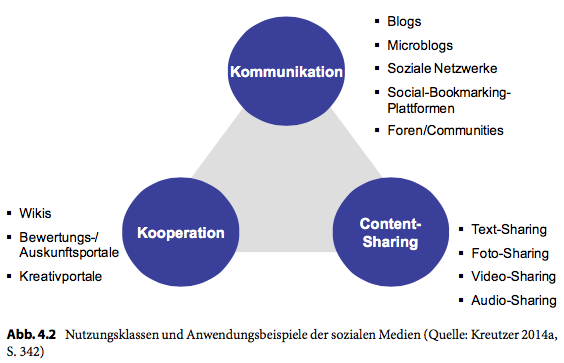
\includegraphics[width=\textwidth]{kapitel/gruppe1_2/bilder/nutzungsklassen}
	\caption{Nutzungsklassen und Anwendungsbeispiele sozialen Medien (Quelle: B2B Online-Marketing und Social Media, S. 152)}
	\label{fig_nutzungsklassen}
\end{figure}

Die Soziale Medien können auf vielfältige Weise genutzt werden. Die Nutzungsklassen, siehe Abbildung \ref{fig_nutzungsklassen} der sozialen Medien können in drei Bereiche aufgeteilt werden:


\begin{itemize}
	\item Kommunikation: Blogs, Microblogs, Soziale Netzwerke, Social-Bookmarking-Plattformen, Foren/Communities
	\item Content-Sharing: Text, Foto, Video, Audio
	\item Kooperation: Wikis, Bewertungs-/Auskunftsprotale, Kreativportale
\end{itemize}

Die Nutzungsklasse \ref{fig_nutzungsklassen} „Kommunikation“ zielt darauf ab, aufbereitete Informationen über private und professionelle Netzwerke bereitzustellen und zu diskutieren.
Ähnlich der Nutzungsklasse „Kommunikation“ zielt auch das „Content-Sharing“ darauf Inhalte zu teilen über spezifische Media-Sharing Plattformen.
Bei der Nutzungsklasse „Kooperation“ steht vor allem die gemeinsame Aufbereitung von Informationen im Mittelpunkt.

Social Media spielt für die Rekrutierung neuer und Erreichbarkeit bestehender HS-Interessierter eine wichtige Rolle. Hierüber können Angebote, Stellenausschreibungen geschehen. Diese können dann verlinkt und geteilt werden. 

Eine Integration in die Website sollte Datenschutzrechtlich vorgenommen werden, bspw. mit der 2-Klick-Technik.




\subsubsection{App als Informationssystem}
\label{android_app_als_is}
Der Trend an Hochschulen geht zu Informationssystemen in Apps bzw. Webapps. Ein allgemeiner Trend dabei ist das Prinzip die Apps so zu entwerfen, dass sie sowohl offline als auch online funktionieren. Dieses Prinzip nennt sich „Offline First“.

\begin{figure}[h!]
	\centering
	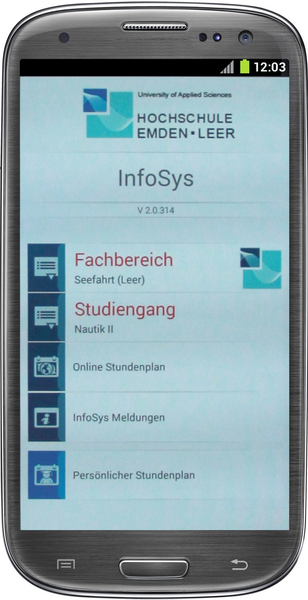
\includegraphics[width=8cm]{kapitel/gruppe1_2/bilder/hsel-androidapp}
	\caption{Android App der HS Emden / Leer}
	\label{fig_hselandroidapp}
\end{figure}
\newpage

Die Hochschule Emden/Leer ist dem Trend gefolgt und hat Anfang 2014 eine Android App im Rahmen einer Projektarbeit vorgestellt, siehe Abbildung \ref{fig_hselandroidapp}. Das Prinzip „Offline First“ wurde dabei berücksichtigt. Ein Hauptaugenmerk wurde auf die Integration von InfoSys und die individuellen Einstellungsmöglichkeiten der Studenten gelegt, um unter anderem den Stundenplan anzupassen.\footcite{hsel_immer_up_to_date_2014}

Da die Entwicklung im Rahmen einer Projektarbeit vonstatten ging, wird es sehr wahrscheinlich bei dieser einen Version und dem einzigen Gerätetyp bleiben.

\begin{figure}[h!]
	\centering
	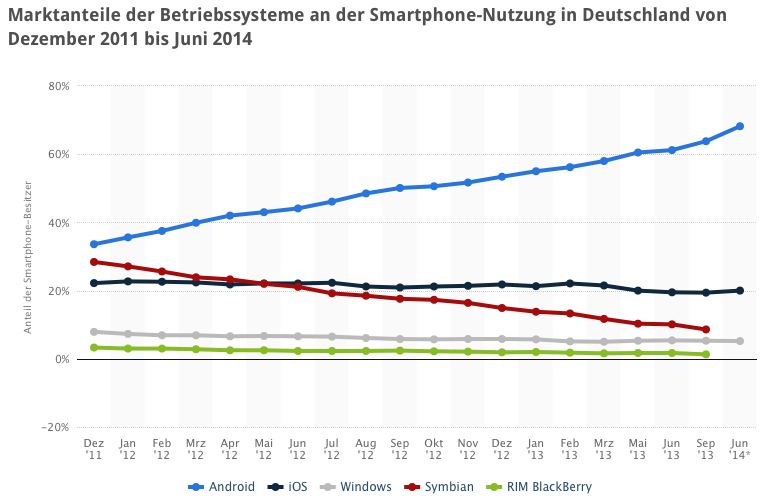
\includegraphics[width=\textwidth]{kapitel/gruppe1_2/bilder/marktanteile}
	\caption{Marktanteile der Betriebssysteme an der Smartphone-Nutzung in Deutschland von 2011 bis 2014\protect\footnotemark}
	\label{fig_marktanteile}
\end{figure}\footnotetext{\cite{statista_markanteile_smartphone_2015}}

An Hand der Marktanteile nach Abbildung \ref{fig_marktanteile}) werden u.a. 20 Prozent iOS Nutzer nicht berücksichtigt und ist daher nicht im Sinne von BYOD, da eine Beschränkung vorliegt. Der Grund dafür liegt an den Unterschieden der Betriebssysteme. Für jedes System muss prinzipiell eine eigene App entwickelt werden. Ein kostengünstiger Lösungsansatz ist der Einsatz ausgereifter Javascript Webapp-Frameworks, wie beispielsweise Sencha Touch\footcite{sencha_touch_2015} und AngularJS\footcite{angularjs_2015}. Die Apps lassen sich so mit jedem Gerät zunächst einmal als Website auf dem Mobilgerät öffnen und mit Hilfe von Cordova/Phonegap\footcite{apache_cordova_2013} ist es weiterhin möglich diese Webapps in den wichtigsten App Stores auszuliefern. Einige Hochschulen bieten solche flexible Webapps an, so zum Beispiel die Hochschule Zwickau.\footcite{whz_webapp_2015}

Nicht nur Flexibilität im Bezug auf Geräteunabhängigkeit wird geschaffen, auch Hürden der Weiterentwicklung werden verringert, weil auf ausgereifte Software gesetzt wird.

Im folgenden werden ein paar Funktionalitäten einiger Hochschul-Apps aufgezeigt.

\paragraph{InfoSys und News}\mbox{}\\\\
An einigen Hochschulen, wie der Hochschule Heidelberg werden unter anderem Hochschulinformationen und aktuelle Nachrichten direkt über eine App ausgeliefert. Die Integration des InfoSys (vgl. Kapitel \ref{fachbereiche_infosys}) und der aktuellen Nachrichten der Hochschule sind vorhanden, jedoch existieren diese Informationen nur für Android Benutzer.

\paragraph{HIS (Notenzugriff, Stundenpläne)}\mbox{}\\\\
\label{paragraph_trends_his}
Die HAW Hamburg und auch die Hochschule Heidelberg ermöglicht in der App den Zugriff auf Stundenpläne, Raumpläne, Prüfungen und Noten.\footcite{akquinet_hawhamburg_2015} Die Hochschule Emden/Leer hat in der Android-App nur den Zugriff auf die Stundenpläne. Die Hochschulen versuchen in Ihren Apps möglichst alle Informationen auszuliefern. Problematisch werden oftmals die Schnittstellen sein. 

\paragraph{Mensa}\mbox{}\\\\ 
Hochschulen haben nicht selten, entweder eine spezielle App nur für die Speisepläne oder sie integrieren die Speisepläne direkt in die eigene Hochschul-App. Die Hochschule Emden/Leer hat derzeit keine spezielle Speiseplan-App. Das Studentenwerk Oldenburg bietet jedoch eine App\footcite{korte_mensaplanol_2009} für iOS an, bei der auch die Hochschule Emden/Leer integriert ist. Derzeit wird laut dem Studentenwerk Oldenburg an einer neuen Webapp für die Speisepläne gearbeitet. Ein Beispiel für ein gelungenes Projekt bietet die Hochschule Osnabrück, sowohl für iOS und Android.\footcite{ncn_studentenfutter_2013}

\paragraph{Gelände-Wegweiser IPS}\mbox{}\\\\
Ein Indoor Positioning System mit beispielsweise Beacons bzw. Triangulation ermöglicht die Standortbestimmung innerhalb von Gebäuden. Das Auffinden eines Raums in neuen bzw. unbekannten Gebäuden mit Hilfe dieser Technologie und einem mobilen Endgerät, ist damit problemlos möglich. 
\newpage
\begin{figure}[h]
	\centering
	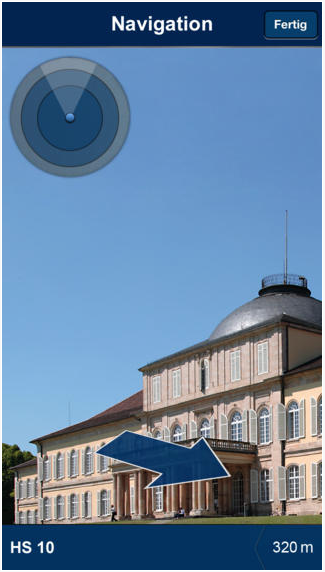
\includegraphics[width=8cm]{kapitel/gruppe1_2/bilder/live-navigation}
	\caption{Hörsaal-Finder der Uni Hohenheim}
	\label{fig_livenavi}
\end{figure}

Die Uni Hohenheim bietet dieses Feature als „Hörsaal-Finder mit Live-Navigation“\footcite{uni_hohenheim_itunes_2013} an, siehe Abbildung \ref{fig_livenavi}.


\section{Abwägung des Einsatzes eines Informationsmanagers an der Hochschule Emden/Leer - JL}
\label{section_einsatz_cio}
\textit{Autor: Julia Lübke}

Das Soll-Konzept analysiert die Ist-Situation um den derweilen Zustand der  Hochschule Emden/Leer zu ermitteln. Daraus lässt sich erkennen, ob es generell einer Verbesserung des Informationsmanagements in der Zukunft bedarf und wo diese anzusetzen sind oder ob noch kein Informationsmanagement besteht und aufgebaut werden muss. Dazu sind verschiedene Aspekte zu beleuchten. Neben der Anforderung des zukünftigen Marketings, den technischen Neuerungen und der darauf folgenden Umsetzung ist zu klären, ob die Hochschule Emden/Leer eine Führung im Bereich des strategischen und operativen Informationsmanagements benötigt.

Im klassischen Informationsmanagement ist dies die Aufgabe eines Informationsmanager, dem sogenannten Chief Information Officer. Wie auf der Abbildung \ref{fig_def_inm} zu erkennen, arbeitet der Informationsmanager dabei als zentrale Schnittstelle zwischen technischen, organisatorischen und wirtschaftlichen Teilbereichen und dient dort als sogenannter Mittler zwischen den verschiedenen Bereichen und untersucht dabei die Informations- und Kommunikationstechniken in allen unterschiedlichen Bereichen um diese sinnvoll einzusetzen. 
\footcite[86]{definition_informationsmanager}

\begin{figure}[h!]
	\centering
	\includegraphics[width=10cm]{kapitel/gruppe3/bilder/definition_informationsmanager}
	\caption{Definition Informationsmanager}
	\label{fig_def_inm}
\end{figure}

\subsection{Analyse des Ist-Zustandes}
\label{subsection_analyse_ist_zustand}

Bezug nehmend auf das Organigramm aus Abbildung \ref{fig_organigramm_HS} der Hochschule Emden/Leer und der Bewertung aus  \ref{bewertung_gewichtung} ist festzuhalten, dass der Hochschule kein klassisches Informationsmanagement zugrunde liegt, sondern ein zentrales Informationssystem. Es werden bereits Informationen verwaltet und weitergegeben, jedoch nicht an zentraler Stelle. Zentrale Systeme, siehe Abbildung \ref{fig_zentrale_systeme}, Kapitel \ref{section_zustaendigkeiten}, sowie unterschiedliche Möglichkeiten werden für alle zur Verfügung gestellt und in Anspruch genommen. 

Es gibt keine Verwaltung, sondern verschiedene Bereiche, die unterteilt sind in Arbeitsgruppen, Abteilungen sowie Rechenstelle und Pressestelle. Weiterhin beinhaltet das Informationssystem verschiedene Prozesse zum Datenaustausch bzw. Datenfluss und Back-up-Transfer aus verschiedenen Systemen.  Die Nutzung des gegenwärtigen Informationssystems wird unterschiedlich stark genutzt oder ausgelastet. 

Von den zentralen Einrichtungen nehmen das Hochschulrechenzentrum und die Bibliothek einen wichtigen Platz in der Hochschule Emden/Leer ein. Das Hochschulrechenzentrum übernimmt derweil viele Aufgaben der Informationsverwaltung und Planung. Doch nicht nur da werden Informationen gesammelt und ausgewertet. Die Hochschule in Emden definiert eine ganze Reihe von Arbeitsgruppen, beispielsweise die Arbeitsgruppe Zahlen, Daten, Fakten, die Kennzahlen der Hochschule und der einzelnen Fachbereiche sammelt und diese auswertet und an gewünschte Stellen weitergibt.  

Aktuell besteht keine erweiterte Vernetzung unterschiedlicher Intranetzsysteme zwischen verschiedenen Hochschulen. Lediglich im Bereich der Bibliothek werden Inhalte an mehreren Standorten gemeinsam genutzt. Abschließend ist zu erwähnen, dass die Hochschule Emden/Leer auch keine Einzelperson oder ein Gremium als zentrale Informationsverwaltung nutzt.


\subsection{Betrachtung des zu erwartenden Soll-Zustandes }
\label{subsection_betrachtung_soll}

Nach Betrachtung der Best-Practice-Beispiele aus Kapitel \ref{chapter_best_practice_beispiele} lässt sich erkennen, dass jede Hochschule und auch Universität den Umgang des Informationsmanagements anders angeht. So spielen verschiedene Faktoren eine Rolle, die an jeder Hochschule/Universität unterschiedlich ausgelegt sind. Ein Vergleich der betrachteten Universitäten mit der Hochschule Emden/Leer zeigt, dass Emden eine wesentlich kleinere Institution ist und somit andere Ansprüche hat und weniger komplexe Strukturen besitzt, als beispielsweise die WWU Münster, die über 40.000 Studierende pflegt. 

Trotz unterschiedlich integrierter Möglichkeiten der unterschiedlichen Universitäten zur Umsetzung des jeweiligen Informationsmanagements, gibt es doch Bereiche, die gleich oder zumindest ähnlich sind. So sind Bibliotheken, Gremien, Ausschüsse, ebenso wie Fachbereiche, das Rechenzentrum und auch das Präsidium Teil einer jeden Hochschule oder Universität. 

Es ist also zu schauen, wo sich das Informationsmanagement als zentrale Informationsquelle ansetzen lässt, um mehrere Bereiche und Bestandteile untereinander zu verbinden. Fakt ist, dass es in Emden bereits drei Arbeitsgruppen gibt, die bestimmte Informationen gewinnen und filtern.  So wäre zu betrachten, wie die Zentralisierung einer übergeordneten Informationsquelle und -weitergabe zu bewerkstelligen wäre und wie der Aufbau einer neuen Struktur die Möglichkeit zur Verbesserung des Informationsaustausches aussehen könnte. 

In Kapitel \ref{subsection_zentralisierung_integration} wird beschrieben, dass die meisten Hochschulen und Universitäten unter einer neu geschaffenen Organisation arbeiten. Dabei spielen das Rechenzentrum, die Bibliothek und die Verwaltung immer eine Rolle in einer solchen Organisation. Kein Konzept ist maßgeschneidert und nicht auf jede Hochschule oder Universität anwendbar.

\subsubsection{Empfehlungen der ZKI bezüglich des Informationsmanagers}
\label{subsubsection_zki}

Neben den verschiedenen Projekten und Einrichtungen, die im Kapitel \ref{chapter_best_practice_beispiele} beleuchtet werden, und aufzeigen, wie mit dem Informationsmanagement umgegangen wird, gibt es noch die Zentren für Kommunikation und Informationsverarbeitung (ZKI) in Lehre und Forschung, die Empfehlungen für Hochschulen bezüglich des Informationsmanagements und besonders Empfehlungen für den Informationsmanager aussprechen.

Blickend auf die Publikation der ZKI basierend auf einer Studie der CIOs und IT-Governance an deutschen Hochschulen aus dem Jahre 2014 wurden über mehrere Jahre von der Kommission für IT-Infrastruktur der Deutschen Forschungsgemeinschaft (KfR) hinweg folgende Empfehlungen für Hochschulen ausgesprochen.

Zwischen 2001 - 2005 gab die KfR folgende Empfehlung:

\textit{" Aufgrund der Relevanz der Informationsverarbeitung für alle Bereiche der  Hochschule wird empfohlen, 
	einen Generalverantwortlichen für Information und  Kommunikation (CIO, Chief Information Officer) 
	in der Hochschulleitung oder ein geeignetes Leitungsgremium mit entsprechenden 
	Entscheidungskompetenzen mit der Entwicklung und  Koordinierung aller IuK-Aufgaben 
	zu betrauen."}\footcite[3]{zki_studie_cio_2014}

Zwischen 2006 - 2010 werden weitere Ausführungen genannt:

\textit{" Integriertes Informationsmanagement ist daher zur wesentlichen Aufgabe bei der Planung des 
	Einsatzes moderner Techniken von Information und Kommunikation für die Hochschulen geworden. 
	Eine solche Planung setzt die Position eines Verantwortlichen für Information und Kommunikation 
	als Mitglied der Hochschulleitung (CIO: Chief Information Officer) voraus, wie er in der Wirtschaft 
	und an verschiedenen Hochschulen bereits etabliert ist."}\footcite[16]{zki_studie_cio_2014}

Die KfR Empfehlungen zwischen 2011-2015 werden noch weiter ausgebaut:

\textit{"In der Hochschulpraxis lassen sich vier unterschiedliche Umsetzungstypen beobachten:  Strategischer CIO mit Leitungsfunktion: Ein Vizepräsident - oder eine Vizepräsidentin - ist explizit für das Informationsmanagement zuständig. Teilweise übernimmt auch der Kanzler die Zuständigkeit für das Informationsmanagement.}

\begin{itemize}
	\item \textit{Strategischer CIO mit Stabsfunktion: Ein Hochschullehrer oder IT-Manager - 
		bzw. Hochschullehrerin/IT-Managerin - im Präsidialstab koordiniert das Informationsmanagement.} 
	\item \textit{Operativer CIO: Der Leiter - bzw. die Leiterin - einer zentralen 
		Informationsinfrastruktureinrichtung fungiert gleichzeitig als CIO der Hochschule.}
	\item \textit{Kollektiver CIO: Die CIO-Funktion wird von einem Lenkungsausschuss mit zwei bis 
		drei Personen ausgeübt, der allerdings - anders als die traditionelle Senatskommission - über 
		unmittelbare Entscheidungsbefugnisse verfügt.}
\end{itemize}
\textit{Jede dieser CIO-Umsetzungsvarianten hat ihre Vor- und Nachteile. Es hängt von den 
	Gegebenheiten an den Hochschulen und insbesondere auch von Personen ab, welche 
	Umsetzung die am besten geeignete ist. Wichtig ist, dass der CIO - in welcher Form 
	auch immer - einen unmittelbaren Zugang zur Hochschulleitung hat und die IT-Belange 
	der gesamten Hochschule strategisch - mit unmittelbarer Richtlinien- und 
	Entscheidungskompetenz - fährt und verantwortet."} \footcite[17]{zki_studie_cio_2014}

Abschließend ist zu sagen, dass die ZKI/KfR einer Hochschule eine zentrale Informationsschnittstelle in Form eines CIOs oder eines CIO-Gremiums empfiehlt.

\subsubsection{Informationsmanager oder Gremium als zentrale Informationsschnittstelle}
\label{subsubsection_cio_gremium}

Der Aufbau eines Informationsmanagements bedarf vieler Schritte und Überlegungen (siehe Abschnitt \ref{begriffsdefinition_inm}). Neben den Veränderungen und deren Umsetzung ist zu klären, ob der bisherige Austausch der Informationen der Hochschule Emden/Leer durch eine zentrale Einrichtung oder einer Einzelperson und entsprechenden Verantwortlichkeiten geregelt werden soll. Um dies in ein reales Szenario zu bekommen, sind die Möglichkeiten aufzuzeigen und ein entsprechend passendes Modell für die Hochschule Emden/Leer zu entwickeln. Dazu werden in Kapitel  \ref{chapter_best_practice_beispiele}, ebenso wie in der Studie der ZKI verschiedene Konzepte des Chief Information Officers (CIO) aufgezeigt. 

Ein einheitliches Konzept ist nicht gegeben, sodass nicht jede Lösung auch passend für die Hochschule Emden/Leer ist. Die betrachteten Universitäten haben ein anderes Anforderungsprofil an ein Informationsmanagement und deren zentrale Leitung als Emden, die wesentlich kleinere und weniger komplexe Strukturen besitzt. Zu den betrachteten Best-Practice-Beispielen lassen sich zusätzlich die Empfehlungen der KfR heranziehen. 

Alle haben gemeinsam, dass das Verwalten der Informationen aus einer Schnittstelle heraus geschieht. Auch dieses Konzept ist für die Hochschule Emden/Leer zu überlegen. Nun stellt sich die Frage, wo diese Schnittstelle anzusetzen ist und wer die Aufgaben übernehmen soll. Verschiedene Möglichkeiten sind hier zu betrachten. Zum einen gibt es das Personenmodell, den CIO, beschrieben in \ref{anforderungsprofil_informationsmanager} und \ref{eingliederung_informationsmanager} der die Schnittstelle bildet, zum anderen gibt es die Möglichkeit eines CIO-Gremiums. 


\textbf{Personenmodell:\newline}
Eine Person wird als Informationsmanager herangezogen und übernimmt die in den Abschnitten \ref{aufgaben_funktionen_informationsmanager},\ref{anforderungsprofil_informationsmanager} und \ref{eingliederung_informationsmanager} angegebenen Aufgaben, die hochschulangepasst sind. Dabei ist zu betrachten, wer diese Aufgabe übernehmen soll. Der CIO kann aus der Privatwirtschaft geordert werden. Dabei ist zu bedenken, dass dafür eine Menge Ressourcen benötigt werden. Neben dem aufwendigen Bewerbungsprozess und der Einstellung erfolgt die Einarbeitungszeit und die Einführung des Informationsmanagements durch den CIO. Als weiterer Punkt sind noch die erhöhten Personalkosten in dieser Zeit zu nennen.

Neben der Möglichkeit einen CIO aus der Privatwirtschaft zu holen, besteht auch die Möglichkeit einen hochschulinternen Mitarbeiter zu involvieren. Der Bewerbungszeitraum und die Einarbeitung verringern sich, da ein bestehender Mitarbeiter die Hierarchie und die Arbeitsweise der Hochschule Emden/Leer bereits versteht und kennt. Allerdings ist nicht zu verachten, dass diese Person, entweder eine Mehrbelastung durch die zusätzlichen Aufgaben des Informationsmanagers tragen muss oder für die vorherige Stelle ein neuer Mitarbeiter gesucht werden müsste, was auch in diesem Fall mit einem erhöhten Kosten- und Zeitaufwand verbunden wäre.


\textbf{Gremiummodell:\newline }
Soll das Informationsmanagement allerdings nicht nur von einer einzelnen Person betrieben werden, ist zu klären, wer diese Aufgabe übernehmen soll. Dazu ist immer in Vergleich zu setzen, welche Parameter greifen. Die Studie der ZKI besagt, Bezug nehmend auf die Abbildung \ref{fig_herkunft_cio_hochschulen}, dass die Gremienmitglieder aus ganz unterschiedlichen Bereichen der Hochschule kommen. Ist dies der Fall und ein Gremium wird ernannt, ist ein Arbeitsaufwand der anfallenden CIO Tätigkeiten auf alle Mitglieder aufgeteilt. So ist der Gesamtaufwand pro Person prozentual geringer als bei einer einzelnen Person, die mindestens 50\% ihrer Zeit in CIO-Aufgaben investiert. 



\begin{figure}[h!]
	\centering
	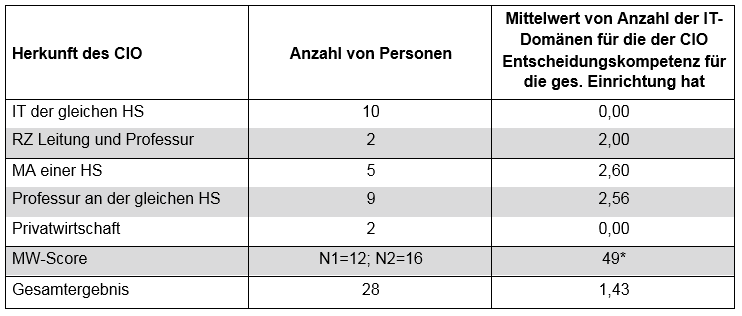
\includegraphics[width=\textwidth]
	{kapitel/gruppe3/bilder/herkunft_cio_hochschulen}
	\caption{Herkunft des CIO an verschiedenen Hochschulen, nach ZKI CIO-Studie}
	\label{fig_herkunft_cio_hochschulen}\footnote{\cite[8]{zki_studie_cio_2014}}
\end{figure}



\subsection{Empfehlung für die Hochschule Emden/Leer}
\label{empfehlung_cio}

Durch stetig wachsende Anforderungen besonders im Bereich der technischen Neuerungen und deren Umsetzung sowie Weitergabe und Verarbeitung von Informationen spricht die KfR seit Jahren Empfehlungen bezüglich eines Informationsmanagers an Hochschulen aus. Durch zusätzliches Betrachten der Best-Practice-Beispiele wird gezeigt, dass jede Hochschule andere Anforderungen besitzt und bezüglich ihrer Größe, Lage und Ansprüche anders mit einem Informationsmanagement umgeht, jedoch alle gemeinsam haben, dass eine zentrale Schnittstelle gebildet wird, die zusammenlaufende Informationen verarbeitet, auswertet und weitergibt. 

Nicht jede Lösung eignet sich dabei für jede Hochschule. In einer Studie der ZKI geht dies ebenfalls hervor. Die Studie befasst sich mit dem Informationsmanager und spricht dabei Empfehlungen für Hochschulen aus. Dabei ist festzuhalten, dass es neben dem Einzelpersonen-Modell auch ein CIO-Gremium-Model geben kann, je nach Bedürfnis der Hochschule. Eine Einzelperson kann hierbei vorteilhafter sein als ein Gremium, dennoch ist zu betrachten, dass ein enormer personeller Kosten- und Zeitfaktor entstehen wird, da nicht zu verachten ist, dass das Aufbauen einer solchen Struktur Jahre in Anspruch nimmt. Es ist daher abzuwägen, ob sich dieser finanzielle Aufwand für die Hochschule Emden/Leer lohnt. 

Da Emden bereits die drei Arbeitsgruppen Zahlen, Daten und Fakten, Web und Moodle besitzt, detaillierter beschrieben in \ref{subsection_arbeitsgruppen_informationsaustausch}, die wichtige Informationen sammeln und verarbeiten, wäre der Hochschule Emden/Leer eine Empfehlung zu einem CIO-Gremium auszusprechen. Durch die bereits existierenden Arbeitsgruppen ist aus jedem Bereich bereits ein Vertreter vorhanden. 

Die Hochschule Emden/Leer ist diesbezüglich schon gut aufgestellt, um weitere Schritte beim Einführen dieses Konzeptes einleiten zu können. Die anfallenden Aufgaben werden auf das gesamte  Gremium aufgeteilt, sodass eine geringere Mehrbelastung entsteht. Abb. \ref{fig_moegliches_gremium} zeigt die Umstellung des Organigramms der Hochschule Emden/Leer, als mögliche Organisation. Das Gremium unterliegt dabei der Hochschulleitung. Da das Rechenzentrum bereits wichtige und zentrale Aufgaben besonders im technischen Bereich übernimmt, wäre es sinnvoll das Gremium aus dem Bereich heraus zu gründen. 

\begin{figure}[h!]
	\centering
	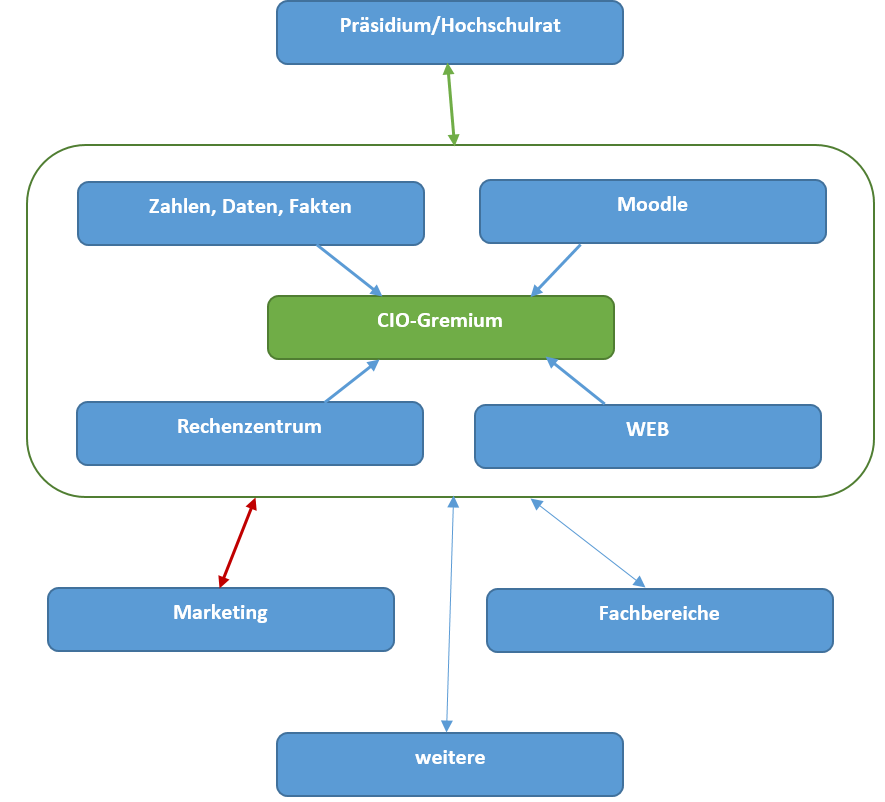
\includegraphics[width=\textwidth]
	{kapitel/gruppe3/bilder/moegliches_cio_gremium}
	\caption{Umstellung/Änderung des Organigramms der Hochschule Emden 	hinsichtlich eines CIO Gremiums}	
	\label{fig_moegliches_gremium}
\end{figure}

In Verbindung mit den drei bereits existierenden Arbeitsgruppen würde sich eine Mischform zwischen strategischem und kollektivem CIO für die Hochschule Emden/Leer anbieten. Das bietet die Möglichkeit sich den gegenebheien der Hochschule anzupassen und ein auf Emden/Leer awäre, dass das CIO-Gremium eng mit dem Marketing zusammenarbeitet und somit von der vorgestellten Möglichkeit Feedback zu sammeln, beschrieben in \ref{feedback} profitieren würde. So können anfallende Probleme direkt diskutiert und Lösungen gefunden werden. 





%\chapter{Best Practice-Beispiele von Informationsmanagement an Hochschulen - LM}
\label{chapter_best_practice_beispiele}
\textit{Autor: Leonhard Massloch}

Wie im Leitbild für ein Informationsmanagement der Universität Kassel festgestellt wird, gibt es für die Organisation der Informationsmanagements in Hochschulen keinen Königsweg. Die Lösungen der Best Practice-Hochschulen seien „vielfältig und hängen von den strategischen Zielen der Hochschule, ihrem Fächerspektrum, ihrer Größe und Pfadabhängigkeiten aus organisatorischen Entscheidungen der Vergangenheit ab.“\footcite{unikassel_leitbild_oD}

Um festzustellen, wie diese vielfältigen Implementierungen in der Praxis aussehen können soll hier anhand einiger Beispiele gezeigt werden, ob und wie andere Hochschulen die aktuellen Trends im Informationsmanagement umsetzen.

\section{Betrachtete Hochschulen}
\label{section_betr_hochschule}
Diese Betrachtung konzentriert sich auf vier Hochschulen, die im Leitbild für ein Informationsmanagement der Universität Kassel als Best Practice-Hochschulen genannt werden: Die Westfälische Wilhelms-Universität (WWU) in Münster, die Technische Universität Dortmund, das  Karlsruher Institut für Technologie und die Universität Ulm.

\subsection{WWU Münster}
Die WWU in Münster ist mit über 40.000 Studierenden\footcite{wwu_profil_2015} die größte der hier betrachteten Hochschulen. In Münster wurde bereits „2003 der IKM-Service institutionalisiert“\footcite[47]{bode_informationsmanagement_2010} um „den Anforderungen an ein integriertes Informationsmanagement im Überlappungsfeld von Information, Kommunikation und Medien (IKM)“\footcite{bode_informationsmanagement_2010} gerecht zu werden. „In diesem Rahmen wurde das Projekt Münster Information System for Re\-search and Organization (MIRO) entwickelt“\footcite[47]{bode_informationsmanagement_2010}, das „über 5 Jahre vor allem mit der Bereitstellung von wissenschaftlichem Personal gefördert“\footcite[7]{vogl_bericht_2013} wurde und „nach einer Verlängerung auf sechs Jahre am 31.12.2011 zu Ende“\footcite[1]{vogl_bericht_2013} ging. Besonders relevant ist das Projekt MIRO deshalb, weil es ein explizites Ziel des Projektes war, „anderen Hochschulstandorten beispielhaft einen Rahmen aufzeigen, den diese auch ohne DFG-Förderung individuell anwenden oder nachnutzen konnten.“\footcite[1]{vogl_bericht_2013}
Bei Betrachtung der Erkenntnisse aus Projekt MIRO sollte jedoch immer beachtet werden, dass die Anforderungen einer Universität der Größe der WWU Münster nicht unbedingt ohne weiteres auf kleinere Hochschulen übertragbar sind.

\subsection{TU Dortmund}
Die Technische Universität Dortmund ist mit rund 32.800 Studierenden\footcite{tu_dortmund_profil_2015} nur unwesentlich kleiner als die WWU Münster. In Dortmund gibt es das IT \& Medien Centrum (ITMC), das sich als „ganzheitlichen Dienstleister für IT-Aufgaben der Technischen Universität Dortmund“\footcite{tu_dortmund_itmc_2015} versteht. Dieser ist aus dem Hochschulrechenzentrum und dem Medienzentrum mit dem Ziel entstanden, „die IT-Kompetenzen der zentralen Einrichtungen zu stärken.“\footcite{tu_dortmund_itmc_2015}

\subsection{Karlsruher Institut für Technologie}
Das Karlsruher Institut für Technologie (KIT) mit über 24.000 Studierenden\footcite{kit_daten_2015} wurde im Jahr 2009\footcite{kit_daten_2015} durch den Zusammenschluss der Universität Karlsruhe mit dem Forschungszentrum Karlsruhe gegründet.\footcite{kit_geschichte_2014}

Am KIT verfolgte das Projekt Karlsruher Integriertes InformationsManagement (KIM) das Ziel, durch Schaffung effizienter organisatorischer Koordinierungs-, Kompetenz- und Servicestrukturen die Zusammenarbeit zwischen den verschiedenen Einrichtungen des KIT zu optimieren, Entscheidungswege zu verkürzen und die Konsistenz der Geschäftspro\-zesse zu erhöhen.\footcite{kit_kim_start_2014}

Im Rahmen dieses Projektes wurde ein Ausschuss für Informationsversorgung und \mbox{-}\nobreak ver\-arbeitung (AIV) eingerichtet, sowie das Medien- und IV-Service-Centrum Karlsruhe (MICK) gegründet, das die Kompetenzen und Ressourcen des Rechenzentrums, der Universitätsbibliothek, der Medieneinrichtungen und der Verwaltung virtuell zusammenführen soll.\footcite{rummele_spaghetti_2006}

\subsection{Universität Ulm}
Die Universität Ulm ist mit über 10.000 Studierenden\footcite{uniulm_universitat_2015} die kleinste der im „Leitbild für ein Informationsmanagement der Universität Kassel“ genannten Best Practice-Hochschulen. In Ulm werden im Kommunikations- und Informationszentrum (kiz) „die Kompetenzen rund um die Informations- und Kommunikationsversorgung der Universität gebündelt.“\footcite{uniulm_wiruberuns_2015}, wobei das kiz die Servicebereiche Bibliothek, Informationstechnik und Medien umfasst.\footcite{uniulm_kiz_2015}

\section{Umsetzung der Trends in den betrachteten Hochschulen}
\label{section_umsetzung_der_trends_in_den_betrachteten_hochschulen}
Im Folgenden soll aufgezeigt werden, auf welche Weise die betrachteten Hochschulen die Trends im Informationsmanagement an Hochschulen umsetzen. Hierbei wird sich auf die Punkte Zentralisierung / Integration, Standardisierung / Serviceorientierte Architektur (SOA), Nutzerorientierung / Serviceorientierung, CIO-Konzept sowie ITIL konzentriert.

\subsection{Zentralisierung / Integration}
\label{subsection_zentralisierung_integration}
Alle betrachteten Hochschulen integrieren mehrere Bestandteile unter einer (oft neu gegründeten) Dachorganisation. Typische Bestandteile dieser Dachorganisation sind das Rechenzentrum, die Bibliothek und die Verwaltung.
An der WWU Münster ist der IKM-Service (Information, Kommunikation und Medien) diese Dachorganisation.\footcite{wwu_ikm_2015}

Dieser bestand bereits vor dem Projekt MIRO\footnote{\cite[8]{vogl_bericht_2013}} und wurde als Rahmen für dieses verwendet.\footnote{\cite[47]{bode_informationsmanagement_2010}}

Der IKM-Service besteht konkret aus dem Zentrum für Informationsverarbeitung (ZIV), der Universitäts- und Landesbibliothek Münster (ULB) und der Universitätsverwaltung (UniV). Er „bündelt die an der WWU vorhandenen Kompetenzen im Bereich Informationsbereitstellung und –verarbeitung in einem virtuellen Verbund mit kooperativer Leitung“.\footcite{wwu_ikm_2015}

Der IKM-Lenkungsausschuss, der sich „aus den Leitungen der beteiligten Einrichtungen sowie dem Prorektor für strategische Planung und Qualitätssicherung“ zusammensetzt, koordiniert die Zusammenarbeit der Bereiche.\footcite{wwu_ikm_2015}

Das ITMC an der TU Dortmund ist unter den betrachteten Dachorganisationen die am wenigsten breit aufgestellte und besteht aus dem Hochschulrechenzentrum und dem Medienzentrum.\footcite{tu_dortmund_itmc_2015}

Das MICK am KIT setzt sich aus dem Rechenzentrum, der Universitätsbibliothek, den Medieneinrichtungen und der Verwaltung zusammen.\footcite{rummele_spaghetti_2006} Die Aufgabe des MICK ist es, „umzusetzen, was der Ausschuss für Informationsversorgung empfiehlt“.\footcite{rummele_spaghetti_2006}

Das kiz an der Universität Ulm integriert IT-Dienste, Medien-Dienste und Bibliotheks-Dienste unter einer gemeinsamen Leitung.\footcite{uniulm_wiruberuns_2015} Außerdem war „der EDV-Betrieb der Verwaltung schon immer im Universitätsrechenzentrum und nicht in einer eigenen EDV-Abteilung angesiedelt. Dieser Aufgabenbereich wurde nach der Auflösung des Rechenzentrums vom kiz übernommen.“\footcite{uniulm_diensleistungen_2015}

\subsection{Standardisierung / SOA}
In Münster wurde im Zuge von Projekt MIRO eine „einheitliche Architektur innerhalb der IT-Komponenten“ angestrebt und als ein „Ansatz zur Erreichung dieses Zieles“ eine „Serviceorientierte Architektur (SOA)“\footcite[51]{bode_informationsmanagement_2010} umgesetzt. Als Gründe für die Einführung einer SOA werden Flexibilisierung, Kostenreduktion und Erhöhung der Wiederverwendbarkeit von IT-Prozessen\footcite[51]{bode_informationsmanagement_2010} genannt. Technisch wird die Informationsinfrastruktur über Server- und Storage-Virtualisierung umgesetzt, da hierdurch eine „flexible und kurzfristige Provisionierung von Komponenten“\footcite[52]{bode_informationsmanagement_2010} ermöglicht wird.
\newpage
Das Projekt MIRO befasst sich in erster Linie mit der „Schaffung einer Infrastruktur für die Nutzung und Verwaltung von (Web-) Services“\footcite[52]{bode_informationsmanagement_2010}, es werden jedoch „generell jede Art von Web-Procedure-Calls (HTTP-Aufrufe, REST-Services etc.) unterstützt.“\footcite[52]{bode_informationsmanagement_2010}

In Karlsruhe ist ein Fokus des Projektes KIM die „technologische Umsetzung einer integrierten Service Orientierten Architektur (iSOA). Hierbei handelt es sich um eine auf Webservices basierende Softwaretechnologie zur Realisierung von Dienstleistungen, bei der die Geschäftsprozesse im Vordergrund stehen“.\footcite{kit_kim_projekt_2012}
Wie auch in Münster steht im Vordergrund, durch flexiblere IT-Strukturen die Kosteneffizienz und Transparenz zu erhöhen und zu einer Beschleunigung der Bearbeitungsprozesse zu führen.\footcite{kit_kim_projekt_2012}

Ein explizites Ziel der Serviceorientierten Architektur ist, dass die „heterogene IT-Landschaft der Fakultäten und Einrichtungen [...] erhalten bleiben und durch einen auf der Web Service Architecture (WSA) basierenden Ansatz zu einem homogenen und hochflexiblen Ganzen zusammengefügt werden“\footcite{kit_kim_projekt_2012} kann.

\subsection{Nutzerorientierung / Serviceorientierung}
Eines der obersten Prinzipien bei der Umsetzung des Projekt MIRO an der WWU Münster war „von Beginn an die konsequente Ausrichtung der Dienstleistungen am Bedarf der Nutzer.“\footcite[19]{vogl_bericht_2013}

Auf diese ausdrückliche Nutzerorientierung führt die Universität auch zurück, dass „ein so umfassendes Projekt wie MIRO bereits von Beginn an wesentliche Ergebnisse generieren konnte und nicht nur auf dem Campus der WWU Anerkennung erzielte.“\footcite[19]{vogl_bericht_2013}

Hierfür wurden u.a. „Ergebnisse ausgewählter Umfragen speziell unter dem Aspekt Informationsverhalten und -bedarf analysiert“\footcite[19]{vogl_bericht_2013} sowie „Bedarfsanalysengespräche mit Wissenschaftlern unterschiedlicher Fachbereiche und Institute geführt“ um „den Status quo im Umgang mit wissenschaftlichen und organisatorischen Informationen [...] zu erfassen“\footcite[19]{vogl_bericht_2013} und „Bedarfe und Verbesserungspotentiale aufzuspüren.“\footcite[20]{vogl_bericht_2013}

\newpage

Der Beirat des ITMC an der TU Dortmund wurde explizit eingerichtet, um „Nutzerorientierung zu 
gewährleisten.“\footcite{tudortmund_itmc_beirat_2013} Als „zentrale Anlaufstelle für alle Fragen 
rund um die Dienstleistungen des ITMC“\footcite{tudortmund_support_service_desk_2013} gibt es 
den Service Desk, der einen umfangreichen Dienstleistungskatalog 
bereitstellt.\footcite{tudortmund_dienstleistungskatalog_2013}

Dort sind auch die Service Level definiert, wobei  die Systeme 24x7 (ausgenommen definierte Zeitfenster für Wartungsarbeiten) und der Support 8x5 zur 
Verfügung 
stehen.\footcite[7]{tudortmund_dienstleistungskatalog_2013}

Für das Projekt KIM-CM (KIM Campus Management), einem Teilprojekt von Projekt KIM, in Karlsruhe gehörte es zu den zentralen Projektgrundsätzen, „alle Anspruchsgruppen im Rahmen von Facharbeitsgruppen und dem Studierenden-Arbeitskreis in das Projekt“\footcite{kit_kim_auswirkungen_2013} einzubeziehen, „so dass die neue Software bestmöglich an den Bedürfnissen aller Anwender und Nutzer ausgerichtet wird. Das Projekt KIM-CM zielt auf eine Optimierung aller Geschäftsabläufe, so dass alle betroffenen Gruppen davon profitieren.“\footcite{kit_kim_auswirkungen_2013}

\subsection{Das CIO-Konzept}
\label{subsection_cio_konzept}
In Münster gibt es keine Einzelperson als CIO. Stattdessen „wurde als Steuerungsgremium der IV-Lenkungsausschuss (IV-L) initiiert“\footcite[59]{bode_informationsmanagement_2010}, der „direkt dem Rektorat zugeordnet“\footcite[59]{bode_informationsmanagement_2010} ist. Die Aufgaben des IV-L sind „u.a. die Sicherung des nutzergerechten und wirtschaftlichen Betriebs des Gesamtsystems und die Festlegung sowie Kontrolle von Zielen und Aufgaben auf zentraler und dezentraler Ebene.“\footcite[9]{vogl_bericht_2013}

Damit ist der IV-L „dem CIO von Unternehmen vergleichbar, dabei allerdings gut an die Gegebenheiten der Universität angepasst.“\footnote{\cite[60]{bode_informationsmanagement_2010}}

Der IV-L setzt sich zusammen aus dem Rektor/der Rektorin oder einem Prorektor/einer Prorektorin, dem Kanzler/der Kanzlerin, dem oder der Vorsitzenden der IV-Kommission, der Leiterin oder dem Leiter des IV-Zentrums sowie der Leiterin oder dem Leiter der ULB, sowie drei weiteren Mitgliedern und deren Stellvertreterinnen und Stellvertreter.\footcite{wwu_ivlenkungsausschuss_2015}
Er trifft sich zweimal pro Semester.\footcite{wwu_ivlenkungsausschuss_2015}

An der TU Dortmund erfüllt der Leiter des ITMC die Funktion des CIO.\footcite[37]{tudortmund_jahrbuch_2009}
Außerdem gibt es den Beirat des ITMC, der mindestens zweimal pro Jahr tagt und Stellung zu dem Entwicklungskonzept des ITMC, der Budgetplanung für das ITMC, dem Dienstleistungskatalog, der Zielvereinbarung und dem Jahresbericht nimmt.\footcite{tudortmund_itmc_beirat_2013}

Auch in Karlsruhe gibt es einen CIO. Dieser „ist KIT-weit für die technische, organisatorische und nutzungsrechtliche Integration und Koordination aller Aktivitäten in den Bereichen Information und Kommunikation zuständig.“\footcite{kit_cio_2015}

In Ulm gibt  es die Position des CIO nicht, aufgrund der starken Integration der unterschiedlichen Informationsdienste kann aber wohl davon ausgegangen werden, dass die Leitung des kiz einen Großteil der Aufgaben übernimmt, die in den Aufgabenbereich eines CIO fallen würden.

\subsection{ITIL}
\label{subsection_itil_best_practice}
Die IT Infrastructure Library (ITIL) findet zwar häufig Erwähnung, nimmt jedoch in der praktischen Umsetzung des Informationsmanagements an den betrachteten Hochschulen keine wichtige Rolle ein.

An der WWU Münster war es eines der Ziele von Projekt MIRO, projektbegleitend „verschiedene Dienstleistungen zu vervollständigen und zu verbessern. Das betrifft die Themen Sicherheit, System- und Netzwerkmanagement, die Einführung von Service-Levels für angebotene Dienste und eine deutlichere Strukturierung der Dienste im Sinne von ITIL (IT Infrastructure Library).“\footcite{unimunster_projekt_miro_2015}.

An der TU Dortmund wurde 2008 für den Service Desk aus Mitteln des Landes NRW Software „mit angepassten ITIL-konformen Frameworks“\footcite{tudortmund_itmc_service_desk_2013} beschafft.
An der Universität Karlsruhe wurde 2007 ein Pilotprojekt durchgeführt.\footcite{grindler_itil_pilot_2007}
In Ulm ist ITIL von den betrachteten Universitäten am stärksten im Einsatz. Eine der Aufgaben der erst 2014 gegründeten\footcite{uniulm_abteilung_service_2014} Abteilung Servicemanagement und Organisation des kiz umfasst „Modellierung und Management von Service-Prozessen (insb. nach ITIL-Standard)“.\footcite{uniulm_abteilung_service_2014}

%\newpage
\section{Zusammenfassung}
Zusammenfassend lässt sich sagen, dass die betrachteten Hochschulen in der Umsetzung des Informationsmanagements zwar oft im Detail unterschiedliche Konzepte verfolgen, in einigen Punkten aber die Gemeinsamkeiten überwiegen.

So setzen alle betrachteten Hochschulen auf eine gewisse Integration von Rechenzentrum, Mediendiensten und oft auch Bibliothek und Verwaltung unter einer zentralen Dachorganisation, die die unterschiedlichen Bereiche koordiniert und von einem CIO oder einem mit den normalerweise mit dem CIO assoziierten Aufgaben betrauten Ausschuss geleitet wird.

Sehr hoher Wert wird generell auf die Nutzerorientierung gelegt. Oft existieren Instanzen, in deren Aufgabenbereich es explizit fällt, diese Nutzerorientierung zu gewährleisten.

Um die heterogenen Anforderungen einer Universität überschaubar umsetzen zu können, setzen einige der betrachteten Hochschulen auf eine Serviceorientierte Architektur.

Bezüglich der Umsetzung von ITIL herrscht in den meisten betrachteten Hochschulen zwar ein gewisser Wille, dieser reicht jedoch nur selten zu einer umfangreichen praktischen Umsetzung.
\chapter{Ist-Situation der Hochschule Emden/Leer hinsichtlich wichtiger Dimensionen - ME, TK}
\textit{Autoren: Marc Enders (ME), Tina Koppermann (TK)}

Im Folgenden wird auf die Ist-Situation an der Hochschule Emden/Leer eingegangen. Durch ein 
Experteninterview mit dem Leiter des Hochschulrechenzentrums sowie weiteren intensiven Recherchen soll 
mit Hilfe der gesammelten Informationen reflektiert werden, ob an der Hochschule bereits ein 
Informationsmanagement betrieben wird. Anschließend erfolgt eine Bewertung und Gewichtung der 
bisherigen Ist-Situation.

Im Folgenden wird auf die Ist-Situation an der Hochschule Emden/Leer eingegangen. Durch ein 
Experteninterview mit dem Leiter des Hochschulrechenzentrums sowie weiteren intensiven Recherchen soll 
mit Hilfe der gesammelten Informationen reflektiert werden, ob an der Hochschule bereits ein 
Informationsmanagement betrieben wird. Anschließend erfolgt eine Bewertung und Gewichtung der 
bisherigen Ist-Situation.

\section{Ziel (TK)}
Mit Hilfe einer Analyse der Ist-Situation an der Hochschule Emden/Leer wird festgestellt, in wieweit bereits 
ein Informationsmanagement besteht. Wenn dies nicht der Fall ist, wird recherchiert, welche Informationen 
zentral gesammelt werden und welche Bereiche in das Projekt \textbf{„Potentielle Neuordnung des 
	Informationsmanagements einer kleineren Fachhochschule auf der Grundlage bestehender Lösungen an 
	deutschen Hochschulen“} mit einbezogen werden müssen.

Wesentliche Fragestellungen, die in diesem Kapitel gelöst werden sollen, sind auf der einen Seite, 
herauszufinden, welche vorhandenen IT-Systeme bereits zentral Verwendung finden und auf der anderen 
Seite, wie Informationen aktuell repräsentiert werden. Des weiteren soll in dieser Analyse Aufschluss darüber 
gegeben werden, ob ein Informationsmanagement an der Hochschule betrieben wird und wie Informationen 
bereits zentral zur Verfügung gestellt werden.

Die Hochschule Emden/Leer ist eine kleine Hochschule mit aktuell 4626 eingeschriebenen Studierenden. Den 
größten Anteil machen die 4303 Studenten vor Ort 
aus.\footcite{hsel_zeitreihe_2014} Die Hochschule beschäftigt 396 
Mitarbeiter.\footcite{hsel_zdf_2015}
\section{Methodisches Vorgehen (TK)}
Ein Hauptbestandteil dieses Kapitels ist der Prozess der Sammlung, Selektion und Prüfung von Fragestellungen, die die Grundlage für ein Experteninterview bilden. Im Rahmen dieser Ausarbeitung wurde sich für die Durchführung eines Experteninterviews entschieden, da hier die Zielgruppe ein Spezialist ist. In diesem Fall ist der Interviewte der Leiter des Hochschulrechenzentrums der Hochschule Emden/Leer, Günter Müller. Das Experteninterview führten die Studierenden Tina Koppermann, Marc Enders und die betreuende Professorin Maria Krüger-Basener mit Günter Müller durch. 

Bei der Erstellung des Experteninterviews wurde auf die Methodik des SPSS-Prinzipes verstärkt reflektiert. Dem SPSS-Prinzip nach Helfferich\footcite[Vgl.][182 ff.]{helfferich_2009} liegt folgendes Vorgehen zur Grunde:

\begin{enumerate}
	\item Sammeln
	\item Prüfen
	\item Selektieren
	\item Subsumieren		
\end{enumerate}

Mit Hilfe des Prinzips zur qualitativen Datenerhebung fand im ersten Schritt das Sammeln von Fragen statt. Diese konnten von allen Kursteilnehmern in einem zur Verfügung gestellten Online-Dokument eingesehen und editiert werden. Bei der Sammlung der Fragen sind insgesamt 62 Fragestellungen zu unterschiedlichen Schwerpunkten aufgenommen worden (siehe Abbildung \ref{fig_auszug_fragen_sammeln}).

\begin{figure}[h!]
	\centering
	\fbox{\includegraphics[width=\textwidth]{kapitel/gruppe2/bilder/auszug_fragen}}
	\caption{Auszug der gesammelten Fragen}
	\label{fig_auszug_fragen_sammeln}
\end{figure}

Nach Abschluss der Sammlung aller Fragen, folgte im zweiten Schritt die Prüfung dieser. Hierbei wurden reine Informationsfragen direkt aussortiert. 

Im darauffolgenden Schritt erfolgte die Selektion der Fragen, indem entsprechend nach Themengebieten kategorisiert wurde. 

Beim Subsumieren wurde für jede Thematik eine Erzählaufforderung gefunden und die Gliederung des Interviewfadens entsprechend erstellt. Wie in Abbildung \ref{fig_farbcode_SPSS} dargestellt erfolgte mit Hilfe eines Farbcodes die farbliche Markierung und Einsortierung der Fragen, entsprechend nach Erzählaufforderung, Checkliste, konkreter Frage und Aufrechterhaltungsfrage. Ein Auszug der farblich aufbereiteten Subsumtion ist in Abbildung \ref{fig_sortierung_fragentyp} zu sehen.

\begin{figure}[h!]
	\centering
	\fbox{ \includegraphics[width=\textwidth]{kapitel/gruppe2/bilder/farbcode_spss}}
	\caption{angewandter Farbcode für das SPSS-Prinzip}
	\label{fig_farbcode_SPSS}
\end{figure}

\begin{figure}[h!]
	\centering
	\fbox{\includegraphics[width=\textwidth]{kapitel/gruppe2/bilder/sortierung_fragentyp}}
	\caption{Sortierung der Fragen nach Fragentyp}
	\label{fig_sortierung_fragentyp}
\end{figure}

Die Visualisierung der Subsumtion fand mit Hilfe des Anwendungsprogramms Microsoft Excel statt. Als Endergebnis ist ein in acht unterschiedliche Themenbereiche gegliederter Interviewleitfaden entstanden (siehe Abbildung \ref{fig_auszug_interviewleitfaden}).

\begin{figure}[h!]
	\centering
	\includegraphics[width=\textwidth]{kapitel/gruppe2/bilder/auszug_leitfaden}
	\caption{Auszug des Interviewleitfadens}
	\label{fig_auszug_interviewleitfaden}
\end{figure}

An einem festgelegtem Interviewtermin ist mit Hilfe dieses Leitfadens das Experteninterview mit Günter Müller durchgeführt worden. Für die Durchführung des Interviews wurde die Online Video Plattform „Adobe Connect“ genutzt. Günter Müller stimmte der digitalen Aufzeichnung zu. Im Anschluss an das Experteninterview erfolgte in der ersten Phase die Analyse der Aufzeichnung auf wichtige inhaltliche Aspekte.

Wie in Abbildung \ref{fig_E-Learning_Transkription} exemplarisch zu sehen ist, wurde in der zweiten Phase durch Transkription die zur Verfügung gestellte Aufzeichnung mit Hilfe der Applikation „Microsoft Word“ überführt, um die im Interview erhaltenen Informationen besser verarbeiten zu können.

\begin{figure}[h!]
	\centering
	\fbox{\includegraphics[width=\textwidth]{kapitel/gruppe2/bilder/E-Learning_Transkription}}
	\caption{Transkription: E-Learning}
	\label{fig_E-Learning_Transkription}
\end{figure}

In der dritten und letzten Phase ist mit Hilfe des Tools „XMind 6“ zu jedem Themenbereich ein entsprechendes Mindmap generiert worden, um somit bei der Recherche schneller auf Besonderheiten eingehen zu können  (siehe Abbildung \ref{fig_E-Learning_MM}).

\begin{figure}[h!]
	\centering
	\includegraphics[width=\textwidth]{kapitel/gruppe2/bilder/E-Learning_MM}
	\caption{Mindmap: E-Learning}
	\label{fig_E-Learning_MM}
\end{figure}

Die Ergebnisse dieser Analyse werden in den folgenden Kapiteln detaillierter beschrieben. 
\section{Zuständigkeiten (TK)}
\label{section_zustaendigkeiten}
In diesem Kapitel wird auf die Zuständigkeiten in Bezug auf die Informationsbereitstellung an der Hochschule näher eingegangen. Es wird dargestellt, welche Ebenen bereits zentral an der Informationsbereitstellung beteiligt sind. Ebenso wird auf die Besonderheiten einzelner Fachbereiche, zentraler Einrichtungen und dem Präsidium detaillierter eingegangen (siehe Abbildung \ref{fig_organigramm_HS}). 

\begin{figure}[h!]
	\centering
	\includegraphics[width=14cm]{kapitel/gruppe2/bilder/organigramm_HS}
	\caption{Organigramm der Hochschule Emden/Leer\protect\footnotemark}
	\label{fig_organigramm_HS}
\end{figure}\footnotetext{\cite{hsel_organigramm_2015}}
\clearpage

Es erfolgt ein Überblick über die IT-Systeme, die sowohl von Mitarbeitern als auch Studierenden verwendet werden (siehe Abbildung  \ref{fig_zentrale_systeme}). Bei einigen zentralen Systemen ist bereits eine Authentifizierung über Single-Sign-On (SSO) gegeben (siehe Kapitel \ref{realisierung_der_serviceorientierung}).\footcite[Vgl.][]{gunter_muller_interview}

\begin{figure}[h!]
	\centering
	\includegraphics[width=14cm]{kapitel/gruppe2/bilder/zentrale_systeme}
	\caption{Zentrale Systeme für Mitarbeiter und Studenten}
	\label{fig_zentrale_systeme}
\end{figure}


\subsection{Fachbereiche}
\label{fachbereiche_infosys} 
Die einzelnen Fachbereiche sind unter anderem durch die Mitgliedschaft in Arbeitsgruppen in den Informationsbeschaffungsprozess involviert.

Alle Fachbereiche verfügen über die Berechtigung, relevante Informationen im System InfoSys\footcite{hsel_infosys_2015} darzustellen. InfoSys ist eine zentrale Plattform zur Darstellung von organisatorischen Informationen. Diese können direkt online auf der öffentlichen Webseite der Hochschule oder in den Eingangsbereichen der jeweiligen Fachbereiche vor Ort über entsprechende Monitore eingesehen werden. Es werden, nach Fachbereich sortiert, die wichtigsten Neuigkeiten als Newsticker dargestellt und der Zugriff auf alle Vorlesungspläne der Fachbereiche wird zur Verfügung gestellt, um so zügig auf organisatorische Inhalte zugreifen zu können (siehe Abbildung \ref{fig_InfoSys}). Aufbauend auf InfoSys wird eine selbst entwickelte Android-App mit dem Namen "'InfoSys App"'\footcite{hsel_infosys_app_2014} zur Verfügung gestellt auf die im Kapitel \ref{android_app_als_is} näher Bezug genommen wird. 

\begin{figure}[h!]
	\centering
	\includegraphics[width=14cm]{kapitel/gruppe2/bilder/InfoSys}
	\caption{Exemplarischer Screenshot vom InfoSys des Fachbereiches Technik\protect\footnotemark}
	\label{fig_InfoSys}
\end{figure}\footnotetext{\cite{hsel_infosys_2015}}

In den nachfolgenden Kapiteln wird auf die Besonderheiten der einzelnen Fachbereiche eingegangen.

\subsubsection{Seefahrt}
Der Fachbereich Seefahrt ist ein relativ kleiner Fachbereich, der nur am Standort Leer vertreten ist. Dieser verwendet kein zentrales System zur Vorlesung und Raumplanung, sondern eine eigenentwickelte Lösung.\footcite{gunter_muller_interview}

\subsubsection{Technik}
Eine Besonderheit dieses Fachbereiches ist es, dass für den Laborbetrieb ein paralleles Netz neben dem zentralen Netz der Hochschule betrieben wird. Da unter anderem der Lehrstuhl „IT-Sicherheit“ eine entscheidende Rolle im Studiengang Informatik bildet, kommt es zu besonderen Konstellationen in Forschung und Lehre. Technik verwaltet das eigene Netz selbst und ist somit autark vom allgemeinen Hochschulrechennetz. Es besteht jedoch eine enge Zusammenarbeit zwischen Technik (im Speziellen E+I) und dem Rechenzentrum, so dass unter anderem gegenseitige Zugriffsrechte bestehen.\footcite[Vgl.][]{gunter_muller_interview} 

\subsection{Präsidium}
\label{praesidium_label}

Das Präsidium, insbesondere mit dem Bereich zentrale Verwaltung, ist über  Arbeitsgruppen in den Informationsbeschaffungsprozess involviert. Zudem verfügt das Präsidium mit einer Stabsstelle über einen zentralen Bereich im Bezug auf die Repräsentation von Informationen. Das Präsidialbüro, welches als Stabstelle fungiert, ist für das Hochschulmarketing und die Presse- und Öffentlichkeitsarbeit zuständig.\footcite{hsel_organigramm_2015}

\subsubsection{Zentrale Verwaltung}
Die zentrale Verwaltung verwendet im Bereich Personalverwaltung und Finanzen ausschließlich SAP als Buchhaltungssystem. Zur Organisation der Lehr- und Vorlesungsplanung wird UNTIS Plus verwendet. Ebenso wird für die Urlaubsplanung, Zeiterfassung und das Gebäudeschließsystem ein eigenständiges System verwendet. Speziell für die Aufbereitung von Kennzahlen und Zahlen kommt eine Eigenentwicklung als BIS (Business Intelligence System) zum Einsatz.\footcite[Vgl.][]{gunter_muller_interview}

\subsubsection{Rechenzentrum}
Das Hochschulrechenzentrum der Hochschule ist stark in die Administration und Pflege der bestehenden Systeme zur Informationsbereitstellung involviert. Neben der Administration von bestehenden Systemen obliegt dem Hochschulrechenzentrum ebenfalls der Endkundensupport.\footcite[Vgl.][]{gunter_muller_interview}

\subsection{Arbeitsgruppen zum Informationsaustausch und zur Informationsbereitstellung}
\label{subsection_arbeitsgruppen_informationsaustausch}
Die Zuständigkeiten an der Hochschule, bezüglich der Informationssammlung, Beschaffung und Aufbereitung von Informationen, ist bereits durch Arbeitsgruppen in wichtigen Bereichen geregelt. Durch das Interview mit dem Leiter des Hochschulrechenzentrums konnte ein Einblick in die bestehenden Gremien geschaffen werden. Diese treffen sich regelmäßig zum Informations-, Wissens- und Erfahrungsaustausch.

Es existieren drei Arbeitsgruppen, welche für die Informationsverteilung in den jeweiligen Bereichen relevant sind:

\begin{itemize}
	\item Zahlen, Daten und Fakten (ZDF)
	\item WEB
	\item Moodle
\end{itemize}

\subsubsection{Zahlen, Daten und Fakten (ZDF)}
ZDF setzt sich zusammen aus den Verwaltungsabteilungen Finanzen, Personal, Presse und Rechenzentrum. Dieses Gremium ist zuständig für die Erstellung und Aufbereitung von Kennzahlen. Dies können zum Beispiel aktuelle Kennzahlen zu eingeschriebenen Studierenden pro Studiengang sein.  ZDF ist für einen Unterbereich der offiziellen Webseite der Hochschule zuständig. Die Kennzahlen und Zahlen werden gruppenbasiert erstellt. Je nach Berechtigung werden Kennzahlen in unterschiedlichen Detailgraden dargestellt. So können Dekane mehr Informationen einsehen, als andere Mitarbeiter. Öffentlich zugänglich sind nur generelle Kennzahlen.\footcite[Vgl.][]{gunter_muller_interview}

\subsubsection{WEB}
Es existiert eine Arbeitsgruppe, welche für die Gestaltung und den Inhalt der öffentlichen Webseite der Hochschule verantwortlich ist. In dieser Arbeitsgruppe sind aus jedem Fachbereich Repräsentanten mit einbezogen. Die Leitung des Web-Teams obliegt dem Präsidialbüro.\footcite[Vgl.][]{hsel_prasidialburo_2013}

\subsubsection{Moodle}
In der Arbeitsgruppe „Moodle“ sind sowohl Repräsentanten aus jedem Fachbereich als auch der Verwaltungsebene involviert. Da das Moodle E-Learning System mittlerweile als ein zentrales Moodle für alle Bereiche eingeführt worden ist, haben die Mitglieder aus den Fachbereichen die Berechtigung, Kurse im Moodle freischalten zu können. Auf die E-Learning Plattform "Moodle" wird detaillierter im Kapitel \ref{paragraph_moodle} eingegangen.\footcite[Vgl.][]{gunter_muller_interview}
\section{Regelung und Handhabung von vorhandenen Informationen (ME)}

In diesem Kapitel wird näher auf das Thema "'Wissensmanagement"' eingegangen. In einem weiteren Teil dieses Kapitels wird auf das Thema "'E-Learning"' näher Bezug genommen. Im letzten Punkt wird dargelegt, welche Sicherheitsaspekte an der Hochschule zum Einsatz kommen.

\subsection{Wissensmanagement}

Der Begriff "'Wissen"' nimmt eine wichtige Rolle im Wissensmanagement ein, denn "'Wissen"' entsteht durch die 
gedankliche Verarbeitung von Informationen im Gehirn (subjektives Gut). Es existieren verschiedene Wissensarten. 
Zum einen gibt es das "'expli-zite Wissen"' welches das Faktenwissen beinhaltet (aus Büchern, Datenbanken, Internet) 
und leicht zu erlernen ist und zum anderen wird nach "'impliziten Wissen"' unterschieden, welches schwerer zu 
erfassen ist, da es das Erfahrungswissen darstellt. Das Erfahrungswissen ist viel schwerer formulier- und 
kommunizierbar als das Faktenwissen.\footcite[Vgl.][]{wissensmangement_infowiss.net_2009}

Näher betrachtet, ist Wissensmanagement die Organisation der Nutzung von Wissen für den Unternehmenserfolg. 
Doch gegenüber dem Informationsmanagement konzentriert sich der Ansatz des Wissensmanagement sehr stark auf 
den Menschen in seiner Funktion als Wissensträger. Häufig kommen IT-Systeme als Werkzeug des 
Wissensmanagements zum Einsatz, mit dem Ziel Wissenverluste zu kompensieren.\footcite[Vgl.][]{wissensmangement_infowiss.net_2009} Wissensmanagement ist eine 
Erweiterung der Informationsmanagementmaßnahmen. Dies bedeutet, dass nicht klar strukturierte Aufgaben, wie zum 
Beispiel Lernprozesse oder die Speicherung von Informationen besser bewältigt werden können.\footcite[Vgl.][]{wissensmangement_vfhinf.oncampus.de_2013}

Auch die Hochschule wird täglich mit dem Erwerb, der Entwicklung, dem Transfer sowie der Nutzung von 
Wissen konfrontiert. Für den Betrieb eines erfolgreichen Wissensmanagementsystems ist ein klares Regelwerk die Voraussetzung. 

Gilbert Probst erstellte 1999 ein theoretisches Modell der "'Kernprozesse des Wissensmangement"', um implizites 
Wissen besser in Unternehmen zu integrieren. Das Modell besitzt die Elemente: Zielsetzung, Umsetzung und 
Bewertung. Im Modell wird zwischen einem "'äußeren Kreislauf"' (strategische Steuerungsaufgaben) und einem 
"'inneren Kreislauf"' (Umsetzung) unterschieden. Im inneren Kreislauf findet durch den äußeren Kreislauf eine 
Ergänzung der Elemente: Zielsetzung (Wissensziele) und Messung (Wissensbewertung) statt. Die inneren Bausteine 
entsprechen den sechs Kernaktivitäten, wie in Abbildung \ref{fig_wissensmanagament_probst} zu sehen ist. Somit 
bilden die acht Bausteine einen vernetzten Managementregelkreis. Zu sehen ist, dass die Kernaktivitäten untereinander 
in Verbindung stehen, jedoch nicht in vorgegebener Reihenfolge vollständig durchlaufen werden müssen. Dennoch 
muss darauf geachtet werden, dass alle Bausteine gleich berücksichtigt werden, da Probleme oft durch die Isolierung 
einzelner Kernaktivitäten entstehen.\footcite[Vgl.][]{wissensmangement_enzyklopaedie-der-wirtschaftsinformatik.de_2012} 

\begin{figure}[h!]
	\centering
	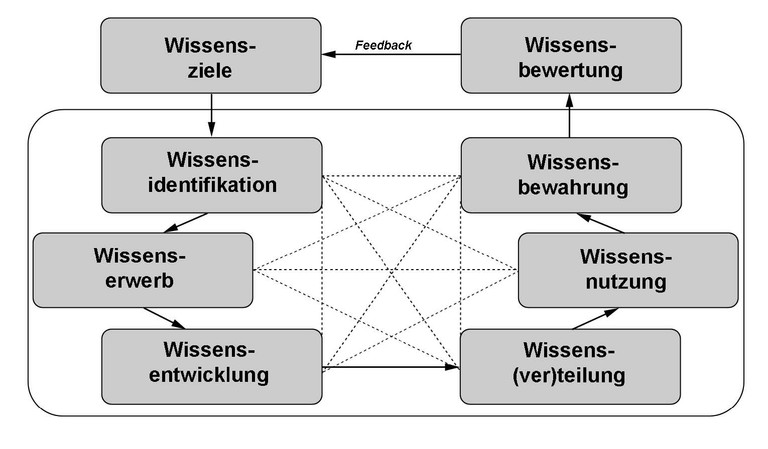
\includegraphics[width=15cm]{kapitel/gruppe2/bilder/wissensmanagament_probst}
	\caption{Bausteinmodell des Wissensmanagement\protect\footnotemark}
	\label{fig_wissensmanagament_probst}
\end{figure}\footnotetext{\cite{wissensmanagement_blog.protechnology.de_2012}}

\subsection{E-Learning}
\label{subsection_e-learning}
E-Learning ist das Lehren und Lernen, welches durch elektronische Medien unterstützt wird. Zum Einsatz kommen digitale Medien, wie zum Beispiel Computer oder Smartphones. Die Übermittlung von Lerninhalten erfolgt über verschiedenste Kanäle wie zum Beispiel das Internet, Computersoftware, Chatsysteme oder durch den Einsatz eines LMS (Learning Management System). Ein sehr bekanntes LMS ist die Plattform Moodle.\footcite[Vgl.][]{e-learning_team025.jimdo.com_2009} In Kapitel \ref{subsubsection_e_learning_plattformen} wird darauf ebenfalls Bezug genommen.

\subsubsection{E-Learning an der Hochschule Emden/Leer}
E-Learning hat an der Hochschule einen hohen Stellenwert, da die Studiengänge Medieninformatik (Online) und seit 2015 Wirtschaftsinformatik (Online) akkreditiert  wurden. Nun soll dargelegt werden, ob in den Präsenzstudiengängen ebenfalls der E-Learning-Prozess Einzug gehalten hat.

\subsubsection{E-Learning in den Präsenzstudiengängen}
Es soll betrachtet werden, in welchen Präsenzstudiengängen E-Learning eingesetzt wird.

Der Fachbereich SAG (Soziale Arbeit und Gesundheit) ist der Vorreiter aller Fachbereiche mit der Einführung eines E-Learning Systems gewesen. SAG setzt mehr als 200 Onlinekurse im Präsenzstudium ein. Für die Anmeldung an verschiedenen Kursen sowie der Klausuranmeldung kommt ein Online-System zum Einsatz.

Es folgt dann der Fachbereich Technik, in dem E-Learning ebenfalls sehr stark verbreitet ist, da die Studiengänge Medieninformatik und Wirtschaftsinformatik als reine Onlinestudiengänge in diesem integriert sind.

Weniger stark wird E-Learning vom Fachbereich Wirtschaft betrieben. Das geringste Nutzungsverhalten ist im Fachbereich Seefahrt zu verzeichnen.

Trotz des unterschiedlichen Nutzungsverhaltens hat E-Learning in allen Fachbereich Einzug gehalten.\footcite{gunter_muller_interview}

\subsubsection[Einsatz von E-Learning-Anwendungen]{Einsatz von E-Learning-Anwendungen in den Präsenzstudiengängen}
In diesem Abschnitt wird erläutert, ob die Anwendungen "'Adobe Connect"' und "'Moodle"' im Präsenzstudiengang eingesetzt werden.\footcite{gunter_muller_interview}

\paragraph{Adobe Connect}\mbox{} \\\\
Adobe Connect ist eine Kommunikationsplattform zur Bereitstellung von Webmeeting- und E-Learning-Inhalten.

Ausschließlich der Fachbereich Technik (E+I) nutzt durch seine Onlinestudiengänge die Plattform Adobe Connect als Medium des visuellen Austausches von Bild und Sprache. In den Präsenzstudiengängen kommt die Plattform nicht zum Einsatz, da der persönliche Austausch von Studierenden und Dozenten in den täglichen Präsenzen stattfindet.\footcite{gunter_muller_interview}
\clearpage

\paragraph{Moodle}\mbox{}\\\\
\label{paragraph_moodle}
Die Hochschule setzt als Lernplattform Moodle ein (siehe Abbildung \ref{fig_moodle}). Moodle ist ein freies objektorientiertes Kursmanagementsystem, welches den Fokus auf E-Learning Inhalte setzt.\footcite{hsel_moodle_2015}

\begin{figure}[h!]
	\centering
	\includegraphics[width=15cm]{kapitel/gruppe2/bilder/moodle}
	\caption{Übersicht Moodle für alle\protect\footnotemark}
	\label{fig_moodle}
\end{figure}\footnotetext{\cite{hsel_moodle_2015}}

Durch den Einsatz von Moodle in allen Fachbereichen wird das volle Leistungsspektrum des Systems ausgenutzt. Folgende Funktionalitäten werden angeboten:

\begin{itemize}
	\item Lernvideos
	\item Vorlesungsskripte
	\item Forum
	\item Kalender
	\item Mail-Connect
\end{itemize}

Für jeden Fachbereich wird der volle Funktionsumfang der Plattform zur Verfügung gestellt, auch wenn nicht jeder Fachbereich jeden Service nutzt.\footcite{gunter_muller_interview} 

\subsubsection{Zentrale Informationsbereitstellung durch Datenlaufwerke}
\label{zentrale_Datenlaufwerke}
Für alle Beteiligten der Hochschule werden drei Datenlaufwerke (siehe Abbildung \ref{fig_zugriff_datenlaufwerke_extern}) auf den Fileservern des eigenen Rechenzentrums zur Verfügung gestellt.\footcite{hsel_moodle_welcome_2015}

\begin{figure}[h!]
	\centering
	\includegraphics[width=15cm]{kapitel/gruppe2/bilder/zugriff_auf_laufwerke_extern}
	\caption{Zugriff auf die Datenlaufwerke von extern \protect\footnotemark}
	\label{fig_zugriff_datenlaufwerke_extern}
\end{figure}\footnotetext{\cite{hsel_moodle_portal_2015}}


\paragraph{Laufwerk Z}\mbox{}\\\\
Auf dem "'Laufwerk Z"' befinden sich die Daten des Home-Verzeichnisses jedes einzelnen Benutzers. Meldet sich dieser an beliebigen Rechnern des internen Rechnerpools an, werden die Inhalte seines Home-Verzeichnisses automatisch eingebunden. Der interne Zugriff auf die eigenen Dateien ist von jedem Rechner des Pools möglich, da servergespeicherte Profile zum Einsatz kommen. Auch von extern können die Studierenden problemlos auf die Ressourcen der Datenlaufwerke zugreifen.\footcite{gunter_muller_interview}

\paragraph{Laufwerk Y}\mbox{}\\\\
Für den gemeinsamen Austausch der Daten wurde das "'Laufwerk Y"' eingerichtet. Hier werden zentral Ressourcen für alle Studierenden und Lehrenden aus Emden zum Austausch zur Verfügung gestellt.\footcite{gunter_muller_interview}
\clearpage
\paragraph{Verzeichnis Lehrende aus Leer}\mbox{}\\\\
Zusätzlich zum Transferlaufwerk wird das Laufwerk "'Verzeichnis Lehrende aus Leer"' zur Verfügung gestellt. Dieses Laufwerk wird zur Bereitstellung von Inhalten (Vorlesungsmaterialien, Skripte, Übungen) verwendet.\footcite{gunter_muller_interview}

\subsubsection{Moodle vs. Datenlaufwerke für Präsenzstudenten}
An der Moodle-Lernplattform melden sich die Nutzer über eine webbasierte Oberfläche am System an. Um Dateien zur Verfügung zu stellen, muss auf der Weboberfläche zu den gewünschten Reitern navigiert werden.

Stellt man die Datenlaufwerke ("'Laufwerk Y"' und das Transferlaufwerk "'Verzeichnis Lehrende aus Leer"') der Moodle-Plattform gegenüber und betrachtet nur den Aspekt des Datenaustausches, so wird deutlich, dass der Dateiaustausch über Datenlaufwerke in Bezug auf Komfort und Aufwand deutlich besser für die Präsenzstudierenden geeignet ist, als die Dateiablage über die Moodle-Plattform. Die über die Datenlaufwerke zur Verfügung gestellten Inhalte können von den Studierenden mit wenig Aufwand intuitiv erreicht werden.

Aus dem Interview mit Günter Müller kristallisierte sich heraus, dass der Fachbereich Wirtschaft die Datenlaufwerke am stärksten sowie der Fachbereich Technik und andere Fachbereiche diese weniger stark nutzen.\footcite{gunter_muller_interview}

\subsection{Sicherheitsaspekte}
\label{subsection_sicherheitsaspekte}
In diesem Kapitel wird auf die bereits verwendeten Sicherheitsrichtlinien an der Hochschule detaillierter eingegangen. Weiterhin wird geprüft, ob ein IT-Service-Management-Prozess  umgesetzt ist.

\subsubsection{Sicherheitsrichtlinien an der Hochschule}
Der Einsatz von Sicherheitsrichtlinien ist ein wichtiges Thema an Hochschulen. Sicherheitsrichtlinien beschreiben die Sicherstellung von Verfügbarkeit, Integrität, Vertraulichkeit und Authentizität von Informationen.\footcite[Vgl.][]{sicherheitsrichtlinien_datenschutz-berlin.de_2008}

An der Hochschule werden, als Basis für die Informationssicherheit, Teile des IT-Grund-schutz-Kataloges umgesetzt. Nicht alle Empfehlungen des BSI (Bundesamt für Sicherheit in der Informationstechnik) sind an einer kleinen Hochschule, wie die Hochschule Emden/Leer es ist,  umsetzbar. Das BSI ist eine nationale Sicherheitsbehörde deren Ziel es ist, die IT-Sicherheit in Deutschland voran zu bringen. Somit ist das BSI ein zentraler IT-Sicherheitsdienstleister des Bundes.\footcite[Vgl.][]{sicherheitsrichtlinien_bsi.bund.de_2015}

An den Serverräumen der Hochschule ist die Umsetzung der IT-Grundschutzmaßnahmen deutlich zu erkennen.
Folgende physikalische Schutzmaßnahmen wurden in den Serverräumen umgesetzt\footcite{gunter_muller_interview}:

\begin{itemize}
	\item einbruchssicher
	\item feuergemeldet
	\item videoüberwacht
	\item Lage der Serverräume im ersten Obergeschoss (Wasserschutz)
\end{itemize}

\subsubsection{Einsatz von ITIL}
Die IT Infrastructure Libary (ITIL) ist eine Sammlung von Best Practises zur Umsetzung eines IT-Service-Management-Prozesses (siehe Kapitel \ref{subsubsection_ITIL}). In diesem Regelwerk werden die für den Betrieb einer IT-Infrastruktur notwendigen Prozesse und Werkzeuge beschrieben.\footcite[Vgl.][]{itil_dxperts.de_2015} ITIL gilt als De-Facto-Standard. Eine Zertifizierung ist nicht für Unternehmen, sondern nur für Personen möglich. Unternehmen können sich nach ISO 20000 zertifizieren lassen.\footcite[Vgl.][]{itil_wirtschaftslexikon.gabler}

Der ITIL-Prozess ist an der Hochschule nicht umgesetzt, da die Personaldecke für die Umsetzung eines 1st- und 2nd-Level Supports nicht gegeben ist.\footcite{gunter_muller_interview}

\subsubsection{Umsetzung von ISO/IEC 27001}
Die ISO/IEC 27001 Zertifizierung wird auf Basis des IT-Grundschutzes vergeben. Durch die Zertifizierung des ISO/IEC 27001 Standards haben Unternehmen, Behörden und Organisationen die Möglichkeit, ihre Bemühungen um Informationssicherheit nach innen und außen zu dokumentieren.\footcite[Vgl.][]{iso_27001_bsi.bund.de_2015}

Das Einsatzszenario ist an der Hochschule nicht gegeben, da für Umsetzung die Personaldichte zu gering ist. Für die Erfüllung der Zertifizierung würde ein riesiger Personaloverhead entstehen.\footcite{gunter_muller_interview}

\subsubsection{Fazit Sicherheitsrichtlinien}
Abschließend ist zu sagen, dass an der Hochschule der IT-Sicherheitsaspekt eine sehr entscheidende Rolle spielt. Als kleine Hochschule ist es auf Grund der Personaldichte nicht möglich, alle Empfehlungen des BSI-Grundschutzes, ITIL und ISO/IEC 27001 umzusetzen. Jedoch sucht sich die Hochschule aus den Regelwerken die Empfehlungen heraus, die auf Grund der Personaldichte umsetzbar sind. Dies bildet eine sehr gute Basis im Hinblick auf das sehr anspruchsvolle Thema IT-Sicherheit.
\section{Repräsentation von Informationen (TK)}
Ein wichtiger Aspekt an Hochschulen ist die Repräsentation von Informationen. Hier spielt sowohl das 
Erscheinungsbild nach außen, als auch die Repräsentation von Informationen innerhalb der einzelnen Bereiche 
eine entscheidende Rolle. Für die interne und externe Kommunikation ist der Bereich "'Presse- und 
Öffentlichkeitsarbeit"' der Hochschule zuständig (siehe Kapitel \ref{praesidium_label}). Nachfolgend wird auf 
die Teilbereiche Studentengewinnung, Corporate Identiy und das Handling von Bewerberdaten näher 
eingegangen.

\subsection{Studentengewinnung}
Wie in Kapitel \ref{praesidium_label} bereits erwähnt, obliegt die Zuständigkeit des Marketings dem 
Präsidialbüro. Generell ist die Studentengewinnung wie folgt aufgeteilt: Zum einen existiert eine zentrale 
Studienberatung, bei der sich Interessenten direkt informieren können und zum anderen werden regelmäßig 
Besuche von Mitarbeitern der Hochschule an Schulen der Region durchgeführt. Mitglieder der Fachbereiche 
berichten vor Ort in den Schulen über die Inhalte der jeweiligen Studiengänge. Neben diesen beiden 
Maßnahmen zur Studentengewinnung verfügt die Hochschule ebenso über Onlinemedien, mit deren Hilfe sich 
die Interessenten über den gewünschten Studiengang und den generellen Ablauf des  Studiums informieren 
können.\footcite[Vgl.][]{gunter_muller_interview}


\subsection{Corporate Identity}
Die Hochschule hat eine Corporate Design-Regelung, die auf der Webseite öffentlich eingesehen werden 
kann. Diese wird vom Bereich Marketing zur Verfügung gestellt und 
gepflegt.\footcite[Vgl.][]{hsel_CD}
\clearpage

Die CD-Reglung umfasst unter anderem einen 
CD-Regelungsguide\footcite{hsel_CD_manual} sowie diverse Vorlagen für PowerPoint 
Präsentationen bis hin zu allgemeinen Logos sowie angepasste Logos für jeden Fachbereich (siehe Abbildung 
\ref{fig_logo_allgemein} und \ref{fig_logo_fb_technik}).

\begin{figure}[h!]
	\centering
	\includegraphics[width=8cm]{kapitel/gruppe2/bilder/hs_logo_allgemein}
	\caption{Allgemeines Logo der Hochschule Emden/Leer\protect\footnotemark}
	\label{fig_logo_allgemein}
\end{figure}\footnotetext{\cite{hsel_CD_manual}}

\begin{figure}[h!]
	\centering
	\includegraphics[width=8cm]{kapitel/gruppe2/bilder/hs_logo_technik}
	\caption{Logo des Fachbereiches Technik\protect\footnotemark}
	\label{fig_logo_fb_technik}
\end{figure}\footnotetext{\cite{hsel_CD_manual}}

\subsection{Handling von Bewerberdaten}
Durch das Interview mit Günter Müller wurde festgestellt, wie das allgemeine Handling von Bewerberdaten aus Sicht des Rechenzentrums stattfindet. 
Der Bewerber meldet sich mit seinen bei Registrierung erstellten Daten am Hochschulinformationssystem (HIS) der Hochschule an und der generierte Account ist nur für die Dauer des Bewerbungszeitraumes aktiv. Im Fall der Nichtannahme des Bewerbers, erfolgt im Anschluss die Löschung seines Accounts. Bei Immatrikulation des Bewerbers wird der vorhandene temporäre Account in einen permanenten Account mit erweiterten Informationseingaben umgewandelt (z.B. Krankenkassendaten). Auf diese Weise wird sichergestellt, dass nur aktive Studenten einen Account zur Verfügung gestellt bekommen.\footcite[Vgl.][]{gunter_muller_interview}
\clearpage
\section{Kooperations-Situation mit anderen Hochschulen (ME)}
\label{section_kooperations_situation}

Das Kooperationsverhältnis mit anderen Hochschulen, Verbänden und Unternehmen spielt auch an der Hochschule Emden/Leer eine sehr entscheidende Rolle, da durch die Kooperation verschiedene Services zur Verfügung gestellt werden.

\subsection{Regionaler Bezug zu Hochschulen (Mitgliedschaften)}
Die Hochschule pflegt ein enges Kooperationsverhältnis mit dem Jade-Hochschulverbund. Über das LBS (Lokale Bibliothekssystem Ostfriesland/Wilhelmshaven) wird auf die gemeinsamen  Bibliotheksbestände zugegriffen.\footcite{jadehs_online_kataloge_2015} Durch ein gemeinsames Promotionskolleg findet ebenfalls eine intensive Zusammenarbeit mit der Universität Vechta statt. Aktuell wird die Kooperation zur Hochschule Osnabrück ausgebaut.\footcite[Vgl.][]{hsel_profil_2015}

Der Rechenzentrumsleiter Herr Günter Müller ist selbst Mitglied des Arbeitskreises LANIT/HRZ.\footcite[Vgl.][]{lanit_mitglieder_2011} Hier treffen die Leiter der Rechenzentren Niedersachsens aufeinander und tauschen ihre Erfahrungen aus. Der Arbeitskreis befasst sich mit Themen der IT-Infrastruktur für Forschung, Lehre und Verwaltung an den Hochschulen Niedersachsens. Zu verschieden Schwerpunktthemen wurden in dem Arbeitskreis entsprechende Arbeitsgruppen eingerichtet.  Ebenfalls werden hochschulübergreifend Projekte durchgeführt.\footcite[Vgl.][]{lanit_home_2014}

Das ZKI (Zentren für Kommunikation und Informationsverarbeitung in Lehre und Forschung e.V.) spielt für die Hochschule eine wichtige Rolle. Ziel dieses Vereins ist es, die Kooperation zwischen den ZKI/Rechenzentren, Meinungs- und Erfahrungsaustausch, sowie die Beratung und Zusammenarbeit mit bildungs- und wirtschaftsfördernden Einrichtungen zu fördern. In den immer wiederkehrenden Tagungen erarbeitet der Arbeitskreis Lösungsvorschläge für aktuelle Probleme der Informationsverarbeitung.\footcite[Vgl.][]{zki_verein_2015} Aktuelle Themen sind z.B. eine Studie über das Thema: „CIOs und IT-Governance an deutschen Hochschulen“.\footcite{zki_beitrag_CIOs_2014}

Durch den Verein DFN (Deutsches Forschungsnetz) wird der Hochschule eine Vielzahl von maßgeschneiderten Kommunikationsanwendungen (DFN-Diensten) zur Verfügung gestellt. Der DFN-Verein ist ein von der Wissenschaft selbst organisiertes Kommunikationsnetz für Wissenschaft und Forschung in Deutschland. Er verbindet Hochschulen und Forschungseinrichtungen miteinander und ist in den europäischen und weltweiten  Verbund der Forschungsnetze integriert.\footcite[Vgl.][]{dfn_home_2015}

\subsection{Kooperation zwischen Unternehmen}
Regional betrachtet, arbeitet die Hochschule mit 82\% der Unternehmen der Region zusammen. Der Vorteil dieser Kooperation ist es, dass zum einen die Studierenden die Möglichkeit haben ihre Fähigkeiten in der Praxis anzuwenden und zum anderen können die Unternehmen das Know-How  der Hochschule nutzen und sinnvoll einsetzen. Der Wissenstransfer, der in der Hochschule erfolgt, bietet den Unternehmen einen erheblichen Mehrwert.\footcite[Vgl.][]{hsel_artikel_kooperation_unternehmen_2014}

\subsection{Eingesetzte IT-Systeme durch Mitgliedschaft im DFN-Verein}
Die angebotenen Dienste des Deutschen Forschungsnetzes sind für den Zweck von Wissenschaft und Forschung maßgeschneidert worden. Ein besonderes Augenmerk liegt hier auf der guten Integration der Dienste in die Prozesse der Hochschulen.  Auf die über den DFN-Verein zur Verfügung gestellten Dienste, die an der Hochschule Emden/Leer zum Einsatz kommen, wird folgend näher eingegangen.\footcite[Vgl.][]{dfn_dienste_2014}

\subsubsection{DFNRoaming/eduroam}
Die Hochschule ist Mitglied des Deutschen Forschungsnetzes (DFN).\footcite{dfn_mitgleider_2012} Durch diese Kooperation nutzt die Hochschule den durch das DFN zur Verfügung gestellten Dienst DFNRoaming/eduroam. Dieser ermöglicht es, registrierten Nutzern über dienst-konforme WLANs Zugang zum Wissenschaftsnetz zur Verfügung zu stellen. Der DFN-Verein betreibt und pflegt die eduroam Förderationsserver in Deutschland. \footcite[Vgl.][]{dfn_roaming_2015} 

In der Abbildung \ref{fig_map_eduroam} ist ein Ausschnitt der weltweiten Lokalitäten der Förderationsserver dargestellt.

\begin{figure}[h!]
	\centering
	\includegraphics[width=\textwidth]{kapitel/gruppe2/bilder/eduroam_map}
	\caption{Standorte der Länder, in denen DFNRoaming/eduroam betrieben wird\protect\footnotemark}
	\label{fig_map_eduroam}
\end{figure}\footnotetext{\cite{weill_cornell_eduroam_2015}}

\subsubsection{GigaMove der RWTH Aachen}
\label{gigamove_rwth_aachen}
Die RWTH Aachen (Rheinisch-Westfälische Technische Hochschule Aachen) stellt eine einfach zu nutzende Möglichkeit zum kurzfristigen Austausch großer Dateien zur Verfügung. Der Datenaustausch kann aus zwei Richtungen erfolgen. Zum einen kann die Nutzer eine Datei hochladen und das System erzeugt einen Link zum Download, zum anderen kann eine Datei angefordert werden, bei der das System einen Link generiert, der zu einem Formular zum Upload der Datei führt. Jeder Nutzer darf Dateien in der Gesamtgröße von 10 GB für einen Zeitraum von 14 Tagen auf den Servern abspeichern. Der von der RWTH Aachen gehostete Dienst GigaMove wird den Nutzern der Hochschule zur Verfügung gestellt.\footcite{hsel_servicelinks_2015} In der Abbildung \ref{fig_rwth_gigamove} ist die Plattform GigaMove der RWTH Aachen dargestellt.

\begin{figure}[h]
	\centering
	\includegraphics[width=\textwidth]{kapitel/gruppe2/bilder/rwth_gigamove}
	\caption{Übersicht der Plattform GigaMove der RWTH Aachen \protect\footnotemark}
	\label{fig_rwth_gigamove}
\end{figure}\footnotetext{\cite{rwth_aachen_gigmove_2015}}

\subsubsection{DFNVideoConference (DFNVC)}
DFNVC (Deutsches Forschungsnetz Video Conference) bietet den Nutzern die Möglichkeit von einem 
PC, einem Raumsystem oder einem Telefon vom Hochschulstandort, durch die Nutzung des 
Wissenschaftsnetzes X-WiN, mit einem oder mehreren Nutzern zu kommunizieren. Die Kommunikation 
findet multimedial statt. Das Wissenschaftsnetz X-WiN ist die technische Plattform des Deutschen 
Forschungsnetzes. Über das X-WiN sind die Hochschulen und Forschungseinrichtungen in Deutschland 
untereinander und mit den Wissenschaftsnetzen in Europa und auf anderen Kontinenten 
vernetzt.\footcite[Vgl.][]{dfn_DFNVideoConference_2014} An der Hochschule wird dieser Dienst 
ebenfalls genutzt\footcite{hsel_shibboleth_auth_2015} und ist über einen Link auf die 
Hochschulwebsite erreichbar.\footcite{dfn_DFNVC_Webkonferenzen_2015}

\subsection{Authentifizierung über Shibboleth-Verfahren und Single-Sign-On}
\label{shibboleth_sso} 

Das Shibboleth-Verfahren (Verfahren zur Verteilten Authentifizierung und Autorisierung für 
Webanwendungen) kommt an der Hochschule zum Einsatz.\footcite[Vgl.][]{hsel_shibboleth_auth_2015}  
Durch dieses Verfahren können Dienste bestimmter Anbieter mit dem Hochschullogin genutzt werden, 
ohne dass bei diesem Anbieter ein neuer Account (Benutzerkennung und Passwort) erstellt werden 
muss. Hierfür existiert an der Hochschule ein Identity Provider Dienst und bei dem entsprechenden 
Dienstanbieter ein Service Provider Dienst.  Beim Aufruf einer Dienstanbieter-Ressource prüft der 
Service Provider Dienst, ob eine bestehende Anmeldesession existiert und leitet die Anfrage an die zur 
Verfügung gestellten Ressourcen weiter, ist dies nicht der Fall, wird der Benutzer an auf Seite 
weitergeleitet, wo er die Lokalität seiner Hochschule auswählen muss. Nach erfolgter Auswahl wird die 
Anfrage an den Identity Provider Dienst der ausgewählten Lokation 
weitergeleitet.\footcite[Vgl.][]{kit_shibboleth_2012} Wie in Abbildung \ref{fig_shibboleth_hs} 
dargestellt, ist dann für eine erfolgreiche Anmeldung die Hochschulkennung erforderlich. Es wird also 
ein zentralisierter Account für die Authentifizierung genutzt.  

\begin{figure}[h]
	\centering
	\fbox{\includegraphics[width=10cm]{kapitel/gruppe2/bilder/shibboleth}}
	\caption{Shibboleth-Login der Hochschule \protect\footnotemark}
	\label{fig_shibboleth_hs}
\end{figure}\footnotetext{\cite{hsel_shibboleth_auth_2015}}
\clearpage
Das Shibboleth-Verfahren ermöglicht den Studierenden und Mitarbeitern die Nutzung folgender Dienste \footcite{hsel_shibboleth_vpn_2015} :

\begin{itemize}
	\item DFNVC (DFN-Webkonferenzen)
	\item Gigamove
	\item video2brain
	\item Springer Link	
	\item WISO	
\end{itemize}

Single-Sign-On, wie in Kapitel \ref{realisierung_der_serviceorientierung} beschrieben, findet in Verbindung mit dem Shibboleth-Verfahren Verwendung. Nach erfolgreicher Authentifizierung ist der Zugriff auf alle Dienstanbieter-Ressourcen, die der Hochschule zur Verfügung stehen, möglich. Es müssen keine weitere Anmeldedaten eingegeben werden.

Für den Zugriff auf die Datenlaufwerke (siehe Kapitel \ref{zentrale_Datenlaufwerke}) wird ebenfalls Single-Sign-On verwendet, da nach der Anmeldung am Client keine weiteren Benutzerdaten zur Authentifizierung eingegeben werden müssen. 
\newpage
\subsubsection{Springer Link}
Studierende und Mitarbeiter der Hochschule haben über die Springer Link-Kooperation Zugriff auf über 40.000 Bücher, 5 Millionen Artikel, 2200 Zeitschriften und 165 Nachschlagewerk.\footcite{springer_springerlink_faq_2015} Die Oberfläche der Springer Link Plattform ist in Abbildung \ref{fig_springerlink_startseite} zu sehen. Springer Link bietet die Möglichkeit die Inhalte als *.pdf herunterzuladen. 

\begin{figure}[h]
	\centering
	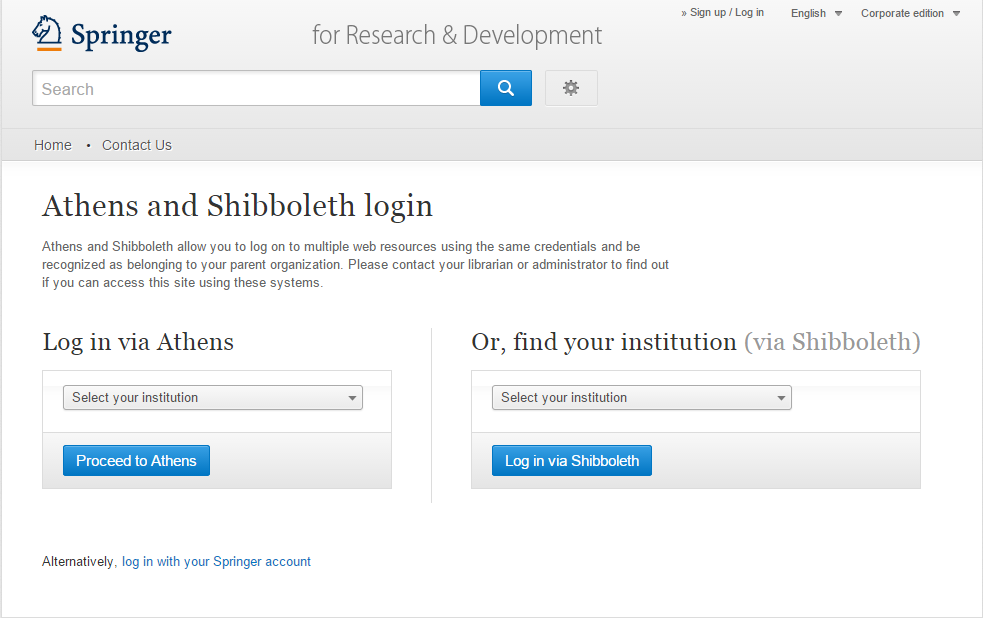
\includegraphics[width=\textwidth]{kapitel/gruppe2/bilder/springerlink_startseite}
	\caption{Springer Link Startseite \protect\footnotemark}
	\label{fig_springerlink_startseite}
\end{figure}\footnotetext{\cite{springer_login_athens_2015}}
\clearpage
\subsubsection{WISO}
Durch das Kooperationsverhältnis mit der GBI-Genios Deutsche Wirtschaftsdatenbank GmbH können die Mitglieder der Hochschule das komplette Angebot an Fachinformationen zu Wirtschafts- und Sozialwissenschaften, technischen Studiengängen und zur Psychologie  nutzen. WISO bietet über 14 Mio. Literaturnachweise, 2100 elektronische Bücher, 130 Mio. Artikel, 700.000 Marktdaten.\footcite{gbi_genios_uber_wiso_2015} Die WISO-Plattform ist in Abbildung \ref{fig_wiso_plattform} zu sehen.

\begin{figure}[h]
	\centering
	\includegraphics[width=\textwidth]{kapitel/gruppe2/bilder/wiso_plattform}
	\caption{Übersicht der WISO-Plattform \protect\footnotemark}
	\label{fig_wiso_plattform}
\end{figure}\footnotetext{\cite{gbi_genios_homepage_2015}}
\newpage
\subsubsection{video2brain}
Seit 2015 ist für alle Mitarbeiter und Studierende der Zugang zum Videostreaming-Portal der video2brain GmbH möglich. Schwerpunkt sind IT- und Kreativ-Themen, Lehrvideos für Fotografen, Grafiker, Web- und Screendesigner. Das Verlagsangebot umfasst mehr als 1700 Video-Trainingskurse. \footcite{adsgmbh_video2brain_2013} In der Abbildung \ref{fig_video2brain_suchergebnis} ist die Weboberfläche nach erfolgreicher Shibboleth-Authentifizierung dargestellt.

\begin{figure}[h]
	\centering
	\includegraphics[width=\textwidth]{kapitel/gruppe2/bilder/video2brain_suche}
	\caption{Übersicht der video2brain Plattform \protect\footnotemark}
	\label{fig_video2brain_suchergebnis}
\end{figure}\footnotetext{\cite{video2brain_homepage_2015}}

\subsection{Support der Dienste}
Für die zentral angebotenen Dienste eduroam, Shibboleth und GigaMove übernimmt die Hochschule den Endkundensupport. Die Mitarbeiter der Hochschule bilden somit die zentrale Support-Schnittstelle und delegieren Anfragen, die vor Ort nicht gelöst werden können, an die entsprechenden Anbieter und Dienstleister weiter.

Diese teilte uns Günter Müller in dem durchgeführten Interview mit.
\section{Bewertung und Gewichtung (TK)}
Abschließend kann gesagt werden, dass Informationen zentral gesammelt werden und wichtige Systeme wie das "'Laufwerk Y"' und die E-Learning Plattform (Moodle) in allen Fachbereichen und in Teilen der Verwaltung zum Einsatz kommen. Durch den starken Kooperationsverbund werden zentrale Dienste, wie Springer Link, WISO und video2brain für die Studierenden und Mitarbeiter dezentral zur Verfügung gestellt. 

Bei der Repräsentation von Informationen nach außen verfügt die Hochschule über eine Pressestelle und eine Marketingabteilung. Es existiert eine feste CD-Reglung für alle Abteilungen und Bereiche. 

Durch diverse Arbeitsgruppen ist der Erfahrungs-, Wissens- und Informationsaustausch für wichtige Bereiche bereits gegeben. Durch die Arbeitsgruppe ZDF, WEB und Moodle werden zentrale Systeme zur Wissenserhaltung und Informationsbereitstellung gepflegt. Dadurch, das die Arbeitsgruppen abteilungsübergreifend agieren, besteht auch zwischen den einzelnen Bereichen eine Schnittstelle, ohne die autarken Fachbereiche einzuschränken. 

Im Bezug auf Serviceorientierung und IT-Sicherheit lässt sich sagen, dass SSO (Single-Sign-On) für einige Bereiche bereits zum Einsatz kommt (siehe Kapitel \ref{realisierung_der_serviceorientierung}). Ebenso werden Teile des IT-Grundschutzes erfolgreich an der Hochschule eingesetzt. Dies sind erste Schritte zum Informationsmanagement, jedoch fehlt grundsätzlich ein zentrales System für den direkten Zugriff und zur Weiterleitung auf weitere Informationssysteme. In Kapitel \ref{immatrikulations_und_pruefungsamt} wird beschrieben, dass in Hochschulen, welche ein Informationsmanagement einsetzen, dieses meistens im Bereich Immatrikulations- und Prüfungsamt (HIS) angesiedelt ist. 
Neben einem  zentralem System fehlt auf der organisatorischen Seite eine Instanz. Wie in Kapitel \ref{cio_text} beschrieben, findet im klassischen Informationsmanagement für Unternehmen das Management häufig durch einen CIO (Chief Information Officer) statt. In Hochschulen wird dies oft durch DACH Organisationen realisiert. 

Auch wenn die Hochschule bereits diverse Arbeitsgruppen einsetzt, so ist diese Instanz des Informationsmanagements bisher unbesetzt. Ein Informationsmanagement, wie es in Kapitel \ref{begriffsdefintion_inm} beschrieben ist, wird derzeit an der Hochschule nicht vollständig praktiziert.
%\chapter{Mögliche Soll-Situation im Hinblick auf die heutigen und zukünftigen Aufgaben - AE, JL, HS}
\label{chapter_sollsituation_INM}
\textit{Autoren: Andreas Ebling, Julia Lübke, Hannes Sprafke}

Eine mögliche Soll-Situation für das Informationsmanagement an der Hochschule Emden/Leer baut auf der Ist-Situation auf, und berücksichtigt die allgemeinen Grundlagen, Besonderheiten von Hochschulen, Trends und Best Practices zum Thema. Wichtige Aspekte an einer kleinen Hochschule sind, neben der großen Autonomie der Beteiligten, auch deren Heterogenität als Gruppe, und die relative Beschränktheit von Ressourcen.

Es werden im folgenden Kapitel also zunächst konzeptionell die Rahmenbedingungen eines möglichen Informationsmanagements hinsichtlich des Endergebnisses betrachtet, sowie die Formalisierung eines Entwicklungsprozesses, der von den Bedingungen der Hochschule profitiert. Im weiteren werden zu diesem Zweck geeignete IT-Systeme betrachtet, sowie erörtert, in welchem personellen Rahmen die Konzeption unter den spezifischen Bedingungen der Hochschule sinnvoll unterzubringen ist.

\section{Marketing - AE}
\label{section_marketing}
Das Marketing hat neben dem typischen Aufgabenbereich der Außenrepräsentation durch die Besonderheiten einer Hochschule auch einen Aufgabenbereich der Innenrepräsentation. Im folgenden werden diese Bereiche getrennt betrachtet.

\subsection{Externes Hochschulmarketing}
\label{subsection_externes_hochschulemarketing}
Das externe Marketing der Hochschule bezieht sich auf die klassischen Marketingaufgaben, das Produkt und die Marke vorteilhaft darzustellen. Im Falle einer Hochschule ist dies die attraktive Darstellung gegenüber zukünftigen Studierenden, Forschungsinteressierten und Geldgebern.

\subsubsection{Webseite}
Zentrales Element bleibt die Hochschulwebseite, die mit aktuellen, offenen Möglichkeiten von HTML 5, CSS 3 und JavaScript den Funktionsumfang einer App erreichen kann, ohne auf spezielle oder spezifische Spezialtechnologien zu setzen. Besonders sei an dieser Stelle die Möglichkeit genannt, mittels Media Queries in CSS Größen und Darstellungsmöglichkeiten von Endgeräten unabhängig von konkreten Betriebssystemen und Hardwareplattformen abzudecken.\footnote{vgl. \cite{w3c_media_queries_url}}

Dies ist vor dem Hintergrund wichtig, dass beispielsweise eine native App für iPhones zwingend durch den Appstore der Firma Apple installiert werden muss\footnote{vgl. \cite{apple_app_distribution_guide_url}}, dessen Nutzungsbedingungen sich für die Hochschule in Form von Kosten oder Inhaltseinschränkungen zu Ungunsten der Hochschule verändern könnten. Mit einer nativen App lässt sich trotzdem nur ein beschränkter Nutzerkreis ansprechen, da mehrere Betriebssysteme und Versionen verbreitet sind.\footnote{vgl. \cite{kantarworldpanel_mobile_betriebssysteme_url}} Sollen mehrere Apps für verschiedene Plattformen gepflegt werden, so ist dies mit zusätzlichen Aufwand, und damit Bindung von Ressourcen verbunden.

Eine Neuauflage der Hochschulwebseite mit aktuellen Möglichkeiten und per CSS an verschiedene Darstellungsgrößen angepasst erreicht dagegen jedes internetfähige Gerät mit Browser. Sollte ein neuer Formfaktor wichtig werden, zum Beispiel der einer Smartwatch, so lässt sich dies über eine Erweiterung des Stylesheets erreichen, ohne eine komplette Neuentwicklung in Auftrag zu geben.

\subsubsection{Soziale Netzwerke}
Soziale Netzwerke wie facebook oder twitter sind nicht eindeutig zu bewerten. Auftritte auf diesen Plattformen können nicht alleine stehen, da nicht jeder einen Account bei einem sozialen Netzwerk hat, benötigen aber durch ständigen Nutzerkontakt eigenständige Pflege und Aufsicht, was an einer kleinen Hochschule Personal bindet.

Für interne Kommunikation und Daten ist ein kommerzielles soziales Netzwerk nicht geeignet, da AGB und Nutzungsbedingungen des Netzwerks mit deutschen Datenschutz- und Urheberrechtsvorgaben, die für eine deutsche Hochschule gelten, in Konflikt stehen können. Auch hier sind Nutzer zu berücksichtigen, die kein Interesse haben, einen Account bei einem sozialen Netzwerk zu eröffnen.

Als Mittel der externen Darstellung ist die Reichweite sozialer Netzwerke potentiell weltweit, was an sich für eine Hochschule mit stark regionaler Bindung \footnote{vgl. \cite{hsel_leitbild_url}} weniger relvant ist. Dennoch sind in subjektiver Wahrnehmung soziale Netzwerke ein wichtiges Kommunikationsmittel und Informationsquelle der Zielgruppe potentieller Studierender. Inwieweit dies speziell für das Einzugsgebiet der Hochschule Emden/Leer gilt ist unbekannt.

Eine Lösung des Konfliktes zwischen Ressourceneinsatz und unbekannter Relevanz ist die öffentlich zugänglichen Informationen der Webseite auch in sozialen Netzwerken zugänglich zu machen. Optimal ist hier, dass kein oder nur geringer Mehraufwand für die zusätzlichen Kommunikationswege entsteht.

\subsubsection{Verteilte Content-Erzeugung}
Im Kontext einer kleinen Hochschule ist die Personalsituation besonders zu berücksichtigen. Es ist nicht praktisch, dass eine oder mehrere Personen zentralisiert die Redaktion aller zu veröffentlichenden Inhalte übernehmen, da relevante Neuigkeiten an mehreren unterschiedlichen Stellen auftreten, und am besten ohne Umweg veröffentlicht werden. Hierzu eignen sich Content-Management-Systeme, die einen Workflow wie in Abbildung 6.1 realisieren.

\begin{figure}[h!]
	\centering
	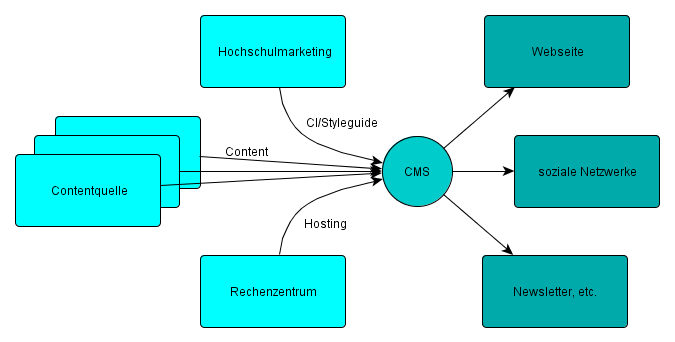
\includegraphics[width=10cm]{kapitel/gruppe3/bilder/verteilter_publishing_workflow}
	\caption{Verteilter Publishing Workflow}
	\label{fig_publishing_workflow}
\end{figure}

Das Hosting wird dabei durch das Rechenzentrum realisiert, während das Hochschulmarketing mit Corporate Identity und Styleguide eine einheitliche Erscheinung der Auftritte leistet. Die Inhalte steuern mehrere, unabhängigen Autoren bei, die mittels unterschiedlicher Berechtigungen und Adressierungen unterschiedliches Publikum erreichen können.
So kann ein unidentifizierter Besucher der Webseite öffentliche, allgemeine Informationen vorfinden, ein angemeldeter Studierender jedoch zusätzlich und prominenter Informationen und Neuigkeiten zu seinem Fachbereich und seinen Kursen.
Weiterhin kann mit einem Content Management System geleistet werden, dass Autoren Inhalte beisteuern und veröffentlichen können, ohne im einzelnen mit den technischen Einzelheiten des Hostings oder des Designs belangt zu werden. Auch können Content Management Systeme Inhalte für weitere Plattformen aufbereiten, zum Beispiel an soziale Netzwerke posten. \footnote{vgl. \cite{content_management_system_patent}}

\subsection{Internes Hochschulmarketing}
\label{subsection_internes_hochschulemarketing}
Im Gegensatz zur Situation in einem Unternehmen genießen einzelne Fachbereiche und Personen in einer Hochschule einen hohen Grad an Freiheit und Autonomie. Daher können in Arbeitsgruppen und Gremien beschlossene Prozesse und Software nicht per Anordnung durchgesetzt werden, sondern müssen nach innen vermarktet werden, um akzeptiert zu werden. Herausfordernd ist hier besonders die Heterogenität, da der technische und fachliche Hintergrund sich unter Mitarbeitern und Fachbereichen erheblich unterscheiden, etwa zwischen technischen und nichttechnischen Fachbereichen.

\subsubsection{Fokussierter Support}
Eine Möglichkeit, Benutzer hin zu einer präferierten Lösung zu leiten ist diese in Präferenzen, Anleitungen und FAQs an erster Stelle und in höherem Detailgrad zu präsentieren. Vielfach wird eine Voreinstellung einfach übernommen, und die erste Lösung zu einer Fragestellung als Referenz angesehen, vergleichbar dem Agenda-Setting.\footnote{vgl. \cite{bonfadelli_medienwirkungsforschung_2015}}

\subsubsection{Schulungen}
Eine weitere Maßnahme ist, Schulungen für die präferierten Lösungen anzubieten, die Vorteile der gefundenen Lösung gegenüber anderen herausstellt. Optimal ist eine solche Lösung transparent, oder aber bietet Alleinstellungsmerkmale, die eine Verwendung aus sich heraus attraktiv erscheinen lassen. Trotzdem kann es vorkommen, dass in Lern- und Umstellungsphasen Lernkurven in der Benutzung absolviert werden müssen. Soll eine Lösung akzeptiert werden, dann muss diese Lernkurve entsprechend begleitet werden.

\subsubsection{Integration}
Eine weitere starke, aber arbeitsintensive Maßnahme ist, die präferierte Lösung stark zu integrieren. Beispielsweise sei die Erstellung von hochwertigen Dokumentvorlagen entsprechend der Corporate Identity für die präferierte Textverarbeitung genannt.

Der Übergang zum fokussierten Support ist hier fließend. Wird die präferierte Lösung an das bestehende System angepasst, so kann von Integration gesprochen werden, wird das System an eine präferierte Lösung angepasst, ist dies fokussierter Support. Beides kann sehr gut gegenseitig ergänzend eingesetzt werden.
\section{Support und Fortentwicklung - AE}
Support und Fortentwicklung hängen hier eng zusammen, da die Fortentwicklung 
hauptsächlich durch die im Support gewonnenen Einsichten über Defizite in Prozessen 
getrieben werden soll. So sollen Diskrepanzen zwischen Erwartungen an das System und 
dessen tatsächlichen Fähigkeiten und Nutzung aufgedeckt und behoben werden.

\subsection{Support}
Supportleistung an einer kleinen Hochschule geschieht häufig direkt und 
unbürokratisch.\footcite{gunter_muller_interview} Dieser ad-hoc-Ansatz bringt 
zwar vielfach schnelle Hilfe, aber nur wenig zuverlässige Informationen über Prozessdefizite.

\subsubsection{Zentrale Dokumentation}
Die Vorteile dieser Art der Hilfeleistung sind für eine kleine Hochschule allerdings evident. 
Der Overhead mehr reglementierter Supportsysteme würde einen unverhältnismäßigen 
Personalaufwand mit sich bringen, und Hilfeleistung verzögern. Die Qualität des 
Supportprozesses selber würde damit sinken.\footcite{gunter_muller_interview}

Notwendig zur besseren Identifizierung von Prozessdefiziten ist allerdings keine 
zentralisierte Supportleistung an sich, sondern lediglich eine zentralisierte Dokumentation 
des geleisteten Supports. Die Abbildung \ref{fig_zentraler_supportlog} verdeutlicht, dass geleisteter Support von 
vollkommen unabhängigen Stellen zentral dokumentiert werden kann.

\begin{figure}[h!]
	\centering
	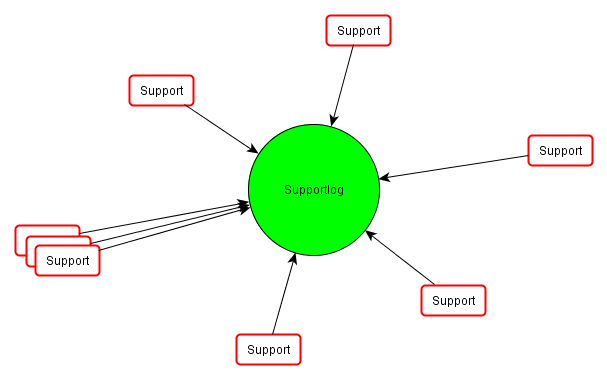
\includegraphics[width=\textwidth]{kapitel/gruppe3/bilder/grafik_supportlog}
	\caption{Unabhängige Supportleister dokumentieren in zentralem Log}
	\label{fig_zentraler_supportlog}
\end{figure}

Es ist dabei unerheblich, ob die Supportleister die Unterstützung als Kern ihrer Aufgabe 
leisten, oder ob es sich um kollegiale Unterstützung bei einem Problem handelt. Gerade 
letztere Information aufzufangen ist wichtig, da diese sonst nur eine sehr schwer 
einzuschätzende Größe bleibt.

Dieser Dokumentationsoverhead ist gering gegenüber dem Overhead eines stark 
reglementierten Supportsystems, erhält alle Vorteile unbürokratischer, schneller 
Hilfeleistung und fängt zusätzlich Informationen über Art und Umfang gelisteten Supports 
auf.

\subsubsection{Knowledge Base}
Aus dem Supportlog kann eine durchsuchbare Knowledge Base aufgebaut werden, die nicht 
nur die allgemeinen Fehlerquellen und Schwierigkeiten von Software im Einsatz beleuchtet, 
sondern ganz speziell die an der Hochschule Emden/Leer in dieser Zusammenstellung 
einmaligen Konfiguration vorliegenden Probleme.

Dadurch kann sehr viel schneller auf spezifische Fehlerszenarien reagiert werden, als dies 
mit allgemeinen Informationen möglich ist, die erst auf die Verhältnisse vor Ort bezogen 
werden müssen.

Auch können aus dem Supportlog FAQs abgeleitet werden, die tatsächlich dem Wortsinn 
nach Listen häufig gestellter Fragen und Antworten darstellen, und nicht was mehr oder 
minder begründet vermutet wird. Eine Diskrepanz mag sich hier durch die Besonderheit von 
Hochschulen ergeben, ein sehr heterogenes Benutzerfeld abzudecken. So mag es 
Nutzergruppen geben, die ein ähnliches Maß an technischer Kompetenz aufweisen wie 
Personal, das ein bestimmtes System betreut, bis hion zu Benutzergruppen, die weit weniger 
oder deutlich andere technische Kompetenz aufweisen.

Auch zeigt sich in den Häufigkeiten bestimmter Probleme, wo spezielle Dokumentation und 
Hilfetexte notwendig sind, die ebenfalls hinterlegt werden können.

Hierzu muss das Supportlog allerdings von einer geeigneten Stelle regelmäßig gesichtet 
werden.

\subsection{Fortentwicklung}
Eine Konzeption kann nur aktuelle Trends und Entwicklungen berücksichtigen. Es ist 
schwierig vorauszuschauen, was die Zukunft danach bringen wird, welche Trends mehr oder 
weniger wichtig sind, und welche Trends darauf folgen werden.

Allerdings ist es keine Frage, dass eine Hochschule länger Bestand hat, und es damit 
sinnvoll ist, Prozesse zu hinterlegen, die neue Trends und Entwicklungen zwar nicht 
vorwegnehmen können, aber deren zeitnahe Entdeckung und Integration ermöglichen.

Auch zeigt sich in der Praxis, dass unvorhergesehene Bedingungen und Ereignisse 
theoretisch gut ausgearbeitete Prozesse und Infrastrukturen übermäßig blockieren können, 
und eine Anpassung geschehen muss. Beispielhaft sei hier für die Hochschule Emden/Leer 
der Trend angeführt, dass Mitarbeiter und Studierende eigene, WLAN-fähige Geräte 
mitbringen und im Netzwerk der Hochschule anzumelden. Das vormals ausreichend 
dimensionierte Netz wurde durch einen Trend unter- oder zumindest 
fehldimensioniert.\footcite{gunter_muller_interview}

\subsubsection{Feedback}
Zur effektiven Begegnung neuer Trends muss an jedem Punkt des Gesamtsystems dem 
Benutzer möglich sein, Feedback zu geben. Mehr noch muss gerade bei neuen oder 
überarbeiteten Prozessen dieses Feedback eingefordert werden, um die Qualität des neuen 
Prozesses oder Tools einschätzen zu können.

Das Feedback gelangt an die zuständige Stelle, muss aber auch zentral gesammelt werden, 
ähnlich wie das Supportlog. Diese Sammlung wird zentral ausgewertet, um verdeckte, 
verteilte Probleme aufzudecken, die sich in Feedback an unterschiedliche Stellen verbergen 
können.

Auf die Auswertung muss, wo sich Probleme zeigen, eine Information der zuständigen Stelle 
folgen, damit eine Verbesserung erarbeitet werden kann. Entsprechend ist die zuständige 
Stelle berechtigt, ein Meeting einzuberufen, damit ihre Eingaben nicht einfach verloren gehen 
können, sondern zwangsläufig mindestens einmal besprochen werden.

\subsubsection{Innovationseingabe}
In den Feedbackprozess eingebettet muss die Möglichkeit für jede Person sein, Innovationen 
aus beliebiger Quelle zu beschreiben, so dass Entwicklungen nicht erst von bestimmter 
Stelle wahrgenommen werden müssen, um erwägt zu werden. Damit kann von beliebiger 
Stelle aus eine Verbesserung in Diskussion gebracht werden.

Damit diese Möglichkeit von Benutzern angenommen wird, muss auf Eingaben angemessen 
schnell reagiert werden. Um eine ernsthafte Reaktion zu gewährleisten, müssen diese 
Vorschläge auch diskutiert worden sein. Daraus ergibt sich ein angemessen kurzer Turnus 
der Auswertung von Support- und Feedbacklog.

\subsubsection{Erfahrungsgetriebene Fortentwicklung}
Aus den Erkenntnissen über Schwachstellen aus dem Supportlog, den Benutzerberichten und 
-bewertungen aus dem Feedbacklog und den Innovationseingaben können nicht nur 
Schwachstellen und Fehler in Prozessen identifiziert werden, sondern auch Trends in der 
Benutzung des Systems erkannt. Da Support und Feedback andauernde Prozesse sind, ergibt 
sich daraus ein selbstregulierendes System, das, wenn die Messgrößen Supportlog und 
Feedbacklog angemessen berücksichtigt werden, evolutionär verbessert wird.

\begin{figure}[h!]
	\centering
	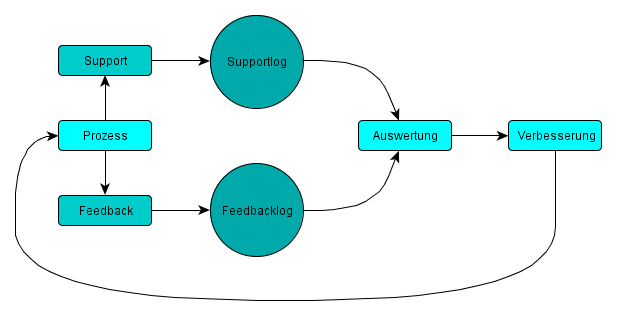
\includegraphics[width=\textwidth]{kapitel/gruppe3/bilder/zyklus_prozessverbesserung}
	\caption{Zyklus der Verbesserung eines Prozesses}
	\label{fig_zyklus_prozessverbesserung}
\end{figure}

Abbildung \ref{fig_zyklus_prozessverbesserung} illustriert den Zyklus folgendermaßen: Ein Prozess existiert und läuft im 
normalen Betrieb. Bei Problemen wird Support geleistet, der im Supportlog vermerkt wird. Zu 
dem Prozess wird zusätzlich Feedback gegeben, das im Feedbacklog festgehalten wird. Beide 
Logs werden ausgewertet und zur Verbesserung des Prozesses herangezogen. Der 
verbesserte Prozess tritt an die Stelle des ursprünglichen Prozesses, der Zyklus beginnt auf 
Basis des verbesserten Prozesses erneut.





















\section{Hard- und Software - HS}

Das folgende Kapitel bezieht sich auf den Teil des Informationsmanagements, den 
Wollnik und Krzmar als Ebene der Informations- und Kommunikationsinfrastruktur 
bezeichnen (vgl. Kapitel \ref{chapter_grundlagen_INM}) Zur Integration eines hochschulweiten 
Informationsmanagements können bezüglich der Hard- und Software mehrere Ansätze 
gefahren werden.

Zum einen kann eine ganzheitliche integrierte Lösung verwendet werden. Die Universität 
Hamburg hat einen vollständigen Neuanfang bezüglich der Campussoftware gewagt mit 
der integrierten Gesamtlösung „CampusNet“ der Datenlotsen Informationssysteme GmbH. 
Die Entscheidung dazu resultierte aus der Zusammenlegung mehrerer Fachbereiche mit 
sehr unterschiedlichen Teillösungen zu einzelnen Fakultäten. Die verschiedenen Teillösungen 
waren größtenteils inkompatibel oder aufgrund von Eigenentwicklung schwer 
wartbar.\footcite[Vgl.][38]{dini_webportale_2007}

Laut Günter Müller, Leiter des Rechenzentrums der Hochschule Emden/Leer, existieren 
an besagter Hochschule derart verschiedene Teillösungen nicht. Auch würden sich derzeit
Eigenentwicklungen bewusst auf vernachlässigbare Systeme beschränken. 
Software würde grundsätzlich für die gesamte Hochschule 
eingesetzt.\footcite{gunter_muller_interview}

Der Einsatz einer integrierten Gesamtlösung zur Beseitigung von Inkompatibilitäten und 
schwer wartbaren Eigenentwicklungen kann somit keine Argumentationsgrundlage sein.
Des Weiteren reicht die in dieser Ausarbeitung getätigte Analyse des Ist-Zustands und 
der Anforderungen nicht aus, um einen vollständigen Anforderungskatalog zu bilden, 
auf dessen Grundlage eine integrierte Gesamtlösung gefunden werden kann.

Stattdessen wird auf eine flexible Lösung gesetzt, welche den Einsatz einzelner 
Fachanwendungen zur Lösung bestimmter Probleme vorsieht. Personelle und 
finanzielle Ressourcen sind dadurch flexibler einsetzbar, auf veränderte Anforderungen 
an eine Lösung kann flexibler reagiert werden und die Abhängigkeit von einem 
Anbieter für alle Anwendungen wird aufgelöst.

Dies ermöglicht eine schrittweise Migration in Form einzelner Projekte. 
Mögliche Strategien dafür werden in Abschnitt \ref{section_migrationskonzepte} näher erläutert. 

\subsection{Kernanforderungen}
Bei Core-Systemen wird weiterhin auf Appliance Lösungen gesetzt. Das minimiert 
Fehlerpotenzial und den operativen Betrieb. \footcite{gunter_muller_interview}

Softwaresysteme laufen auf virtuellen Maschinen. Die bessere Hardwareauslastung 
und Möglichkeit der automatisierten Administration kann finanzielle und 
personelle Ressourcen sparen.\footcite[Vgl.][198]{baun_servervirtualisierung_2009}
Die Systeme sind somit weniger abhängig von der Hardware, was dessen Austausch 
erleichtert. Netzwerkanbindung, Rechenleistung und Speicherkapazität sind somit 
flexibler an sich verändernde Anforderungen anpassbar.

Die eingesetzte Software soll in die Systemlandschaft integrierbar, lösungsorientiert und 
möglichst barrierefrei sein. Um weiterhin verschiedene Teillösungen und Eigenentwicklungen 
zu vermeiden, sollte bei neu einzuführenden Systemen immer geprüft werden, ob bereits 
eine brauchbare Lösung am Markt exisitert.

Da auch das Übertragungsmedium entscheidend zur Erfüllung 
von Informationsbedarfen ist, wie in Abschnitt \ref{subsection_koordination_informationslogistik} 
näher erläutert wurde, soll der Zugang zu Informationen möglichst unabhängig von 
Client-seitig eingesetzten Systemen sein bzw. Unterstützung für möglichst viele 
Zugriffsarten bieten. Diese Freiheit in der Wahl des Mediums unterstützt den Ansatz der 
Freiheit in Forschung und Lehre.

Eine Client-seitige Systemunabhängigkeit kann durch Webanwendungen im Sinne des 
Ansatzes Software as a Service (SaaS) erreicht werden. Um möglichst alle gängigen Browser 
und Endgeräte zu unterstützen, sollten die Anwendungen den Standards des World Wide 
Web Consortiums (W3C) und, soweit möglich, dem Ansatz responsive design gerecht werden. 
Dadurch kann auch dem Trend bring your own device Rechnung getragen werden, wie in 
Abschnitt \ref{netzinfrastruktur_consumerization_und_byod} näher erläutert wurde.

\subsection{Bereichsübergreifende Basissysteme}
Auch wenn eine Hochschule bestimmte Besonderheiten aufweist - vgl. Abschnitt \ref{anwendung_des_inm_auf_hs} - 
fallen dort informationstechnologische Aufgaben an, für die eine zentrale IT-gestützte 
Lösung geschaffen werden kann. Das verringert redundante Daten und Systeme, sowie 
administrative Aufwände. Im folgenden werden Lösungen für einzelne Aspekte des 
Informationsmanagements aus IT-Sicht vorgestellt, die in allen Aufgabenbereichen von 
Hochschulen genutzt werden können. Weiterhin dienen die Lösungen teilweise als Grundlage 
für spezialisierte Systeme oder ermöglichen hilfreiche Erweiterungen dieser.

\subsubsection{Identity Management}
Um die Anzahl an verschiedenen Accounts zu minimieren, sollten die Benutzer zentral gepflegt werden. 
Dies kann in einem Verzeichnisdienst, wie dem bereits eingeführten Active Directory\footcite{gunter_muller_interview}
geschehen. Die Authentifizierung für ein System findet dann nicht am jeweiligen System selbst statt, sondern 
geschieht mit Hilfe des Verzeichnisdienstes. Vorteil ist, dass die Benutzenden sich nur einen Anmeldenamen 
zzgl. Kennwort merken müssen, um sich an den verschiedenen Systemen anzumelden. Weiterhin gilt eine 
Aktualisierung von Informationen global, wodurch Inkonsistenzen aufgelöst werden.

Davon ausgenommen dürfen Systeme sein, deren spezielle Sicherheitsanforderungen nicht mit diesem Konzept 
vereinbar wären. Auch muss die Authentifizierung gesichert geschehen und eine regelmäßige Kennwortänderung 
forciert werden. Auf bestehende Sicherheitsaspekte wurde in Abschnitt \ref{subsection_sicherheitsaspekte} bereits 
eingegangen.

Zuzüglich zum zentralen Verzeichnisdienst ist auch ein SingleSignOn Mechanismus 
empfehlenswert\footnote{siehe Abschnitt \ref{subsubsection_identitatsmanagement}}, 
wie es an der Universität Augsburg durch das System Webauth umgesetzt ist.\footcite[Vgl.][206]{digicampus_2009}

Die an der Hochschule Emden/Leer eingesetzten Websysteme sollen, soweit möglich, vollständig auf SSO umgestellt werden, um dem Benutzer eine möglichst integrierte Landschaft zu bieten. Dies gilt dann auch für einzuführende Systeme. Weiterhin sollte jedes System aus Sicherheitsgründen insofern angepasst werden, dass auch ein SingleSignOff möglich ist.\footcite[Vgl.][150]{kloetgen_2012} Diese zentrale Abmeldung soll gewährleisten, dass die Benutzenden auf allen Systemen, auf denen sie sich bewegt haben, mit einem Klick abgemeldet sind. Der Diebstahl von Websessions bzw. die Fremdnutzung durch Benutzer, die einen Computer anschließend nutzen, kann damit vermieden werden.

Die meisten Systeme bieten eine Benutzerdatenpflege durch den Benutzer selbst an. Diese muss auf den einzelnen Systemen ausgeschaltet sein. Die Benutzenden sollten dennoch die Möglichkeit haben ihre Daten eigenständig zu ändern, allerdings ausschließlich über ein zentrales Formular. So wird ein konsistenter Datenbestand gesichert. Insofern die Informationen in anderen Systemen benötigt werden, müssen diese vom zentralen System wiederkehrend angefordert oder, wenn die Daten im System persistiert sein müssen, automatisiert und über gesicherte Verbindungen verteilt werden.

Ein weiterer Vorteil zentraler Benutzerdaten ist, dass diese zentral ausgewertet werden können. Informationen über Personen können mit Informationen anderer Art aus anderen Systemen angereicht werden um diese weiterzuverwenden. So können automatisierte Reports über Forschungsprojekte erstellt werden, Expertisen zu bestimmten Themen identifiziert werden oder Verknüpfungen von Personen zu verwaltungstechnischen Aufgaben bereitgestellt werden, wie zum Beispiel die Exmatrikulation. Die Umsetzung ist dabei individuell an die Gegebenheiten und Informationsbedarfe der Hochschule anzupassen. Aus diesem Grund wird die technische Lösung eine Individuallösung werden. Diese Individuallösung sollte ein Teil Campus Portals werden, auf das in Abschnitt \ref{subsubsection_campus_portal} eingegangen wird. 

\subsubsection{Geschäftsprozesse}
+Trotz der Freiheit in Forschung und Lehre gibt es an Hochschulen Geschäftsprozesse, die in der Regel immer gleich ablaufen. Bei verstärkter Prozessorientierung werden außerdem vermehrt solche Prozesse entstehen. Ein häufiges Problem bei Geschäftsprozessen ist, dass Personen unterschiedlichster Bereiche involviert sind und die Prozesse häufig nicht transparent genug sind.\footcite[Vgl.][12]{becker_prozesse_2010}

Hier empfiehlt sich der Einsatz von Business Process Management (BPM). BPM dient der Identifizierung, Dokumentation und Verbesserung von Prozessen. Die allgemeine Herangehensweise ist dabei folgende. Nach dem Identifizieren möglicher Prozesse werden diese modelliert, konkretisiert und digitalisiert. Tool unterstützen beim Durchlaufen der digitalisierten Prozesse. Der Verbesserungsprozess, sprich die Anpassung der Prozesse, findet kontinuierlich statt.

Die Modellierung der Prozesse im ersten Schritt sollte auf abstraktem Niveau stattfinden. Dies erleichtert den Einstieg und macht Verbesserungspotenziale sichtbarer. In der WWU Münster wurde dafür die PICTURE Methode verwendet.\footcite[Vgl.][16]{becker_prozesse_2010} Wichtig ist die Einbeziehung der Prozessbeteiligten. Abschnitt \ref{section_changemanagement} setzt sich mit den Besonderheiten des Change Managements an Hochschulen detaillierter auseinander.

Im zweiten Schritt kann der ggf. angepasste Prozess konkretisiert und in Form des Industriestandards Business Process Model Notation (BPMN) digital notiert werden. Ein Client-Tool zur Erstellung von BPMN ist das Activiti BPMN 2.0 Eclipse Plugin.\footcite{eclipse_bpmn2_modeler}

Mit Hilfe der zentralen Business Process Management (BPM) Platform activiti können die Prozesse aktiv den Workflow verbessern, Konsistenz wahren und zeitliche Ressourcen sparen.  Die Plattform ermöglicht REST Anfragen, wodurch die Prozessinformationen auch in andere Applikation integriert werden können. Der Activiti Explorer ermöglicht den voll funktionalen Zugriff via Weboberfläche. Somit wird der Kernanforderung SaaS Rechnung getragen. Weiterhin ist Activiti Open Source und somit ausbau- und anpassungsfähig.\footcite{activiti_website}

Durch activiti wird es möglich sein die Automatisierung von einzelnen Prozessen Stück für Stück voranzutreiben indem manuelle Aufgaben gegen Automatismen ersetzt werden. Einzelne Teile des Workflows können dann automatisiert Scripte starten, E-Mails verschicken und ähnliches und somit stückweise die manuelle Bearbeitung reduzieren. Durch Definition von Pflichtfeldern für einzelne Prozessschritte können vorab benötigte Informationen festgelegt werden, sodass Nachfragen vermieden werden.

\subsubsection{Content Management}
Um den wachsenden Anforderungen in Bezug auf Content Management genüge zu tun, wurde an der WWU Münster das Enterprise Content Management System Alfresco eingeführt. Auch an einer kleinen Hochschule kann ein solches System eingesetzt werden. Alfresco bietet diverse Vorteile. Die für dieses Konzept Relevanten werden hier kurz aufgelistet:\footcite[Vgl.][47 ff.]{kloetgen_2012}

\begin{itemize}
	\item Unterstützung für mobile Endgeräte
	\item Anpassungs- und ausbaufähig
	\item diverse Zugriffsmöglichkeiten zur Nutzung innerhalb bekannter Standardanwendungen
	\item Publikation in sozialen Netzwerken
	\item Unterstützung verschiedener Standardschnittstellen
	\item Activiti Workflow Engine
	\item Metadaten
\end{itemize}

Alfresco bietet damit die ideale Grundlage verschiedenste Informationen zu verwalten, sowie die Unterstützung des vollständigen Dokumenten-Lifecycles: von der Erstellung über die Bereitstellung bis zur Archivierung.

Die Art des Zugriffs auf Dokumente ist dynamisch dank der Unterstützung zahlreicher Standards. Somit kann eine Integration des Zugriffs auf Dokumente, angepasst an die jeweiligen Anforderungen eines benutzenden Systems, geschehen. Ein Dokument, welches an verschiedenen Orten auf verschiedene Arten bereitgestellt werden soll, kann dank Alfresco zentral aktualisiert werden. Die zugreifenden Systeme erhalten immer genau den Lifecyle-Version des Dokuments, der für sie vorgesehen ist.

Dank der integrierten Versionierung entfällt außerdem der aufwendige Wiederherstellungsprozess bei Dateisystem-basierten Sicherungen.

Durch die Möglichkeit Metadaten anzugeben, wird der Weg für eine brauchbare Dokumentensuche geebnet. 
Diese kann in die integrierte Gesamtsuche einbezogen werden.\footnote{siehe Abschnitt \ref{subsubsection_integrierte_gesamtsuche}}

\subsection{Spezialsysteme}
Unter Spezialsystemen sind hier Softwarelösungen zu verstehen, die bei speziellen Aufgaben im Hochschulalltag unterstützen sollen, wie zum Beispiel die Bereitstellung von Lehrmaterial oder die Evaluation von Kursen.

\subsubsection{Lernplattform}
Die Hochschule Emden/Leer setzt bereits erfolgreich und in allen Fachbereichen das System moodle als Lernplatform ein.\footcite{gunter_muller_interview} 
Die Nutzung der Funktionen variiert dabei jedoch zwischen den einzelnen Fachbereichen.\footnote{siehe Abschnitt \ref{subsection_e-learning}}
Solange moodle die Anforderungen der Hochschule an eine Lernplattform erfüllt, besteht kein Grund das System auszutauschen.

Neben den bereits genutzten Standardfunktionen ist moodle ausbaufähig.

Beim Aufruf von moodle soll die Authentifizierung durch einen SSO Mechanismus geschehen. Für das Lernraumsystem moodle gibt es bereits ein SSO Plugin.\footcite{macklin_moodle_sso_plugin} Integriert werden sollte, wie in Kapitel 6.3.2.1 erläutert, dann auch ein Single-Sign-Off Mechanismus.

Statt der Stammdatenänderung via moodle wird der entsprechende Menüpunkt ausgeblendet werden bzw. die Benutzenden auf ein zentrales Formular weiterleiten, um persönliche Informationen zentral und damit konsistent zu halten.

Die in den Kursen zur Verfügung gestellten Dateien jeglicher Art werden in Alfresco gepflegt und von moodle angebunden. Die entsprechenden Schnittstellen und Plugins existieren bereits auf dem Markt und müssen somit nicht neu entwickelt werden.

Vorteil der Integration von Alfresco in moodle ist, dass damit die Vorteile Alfrescos zur Dokumentenverwaltung genutzt werden können. In moodle kann dann eine bestimmte Version oder die jeweils aktuellste referenziert werden. Bei den Dokumenten kann es sich um Textdokumente, Audio- oder auch Videodateien handeln. Durch Alfrescos Unterstützung für mobile Endgeräte wird den Zugreifenden die Möglichkeit gegeben, ein Dokument auf verschiedensten Endgeräten anzuzeigen bzw. wiederzugeben. Außerdem können dank Alfresco diese Dokumente nicht nur innerhalb von moodle via Weboberfläche aufgerufen werden, sondern über verschiedene Medien angebunden werden, zum Beispiel via Filesystem in Form eines Netzwerk-Shares. 
Damit wird eine Freiheit in der Wahl des Übertragungsmedium gewährleistet.\footnote{siehe Abschnitt\ref{subsection_koordination_informationslogistik}}

Ein mögliches Migrationskonzept wird in Abschnitt \ref{subsubsection_changemanagement_alfresco} erläutert.

\subsubsection{Publikationen}
Um Wissenschaftler bei der Publikation von Zeitschriften zu unterstützen, kann die Plattform Open Journal System (OJS) eingesetzt werden, wie es auch in der WWU Münster getan wird. Es bietet die Möglichkeit elektronische Zeitschriften zu verwalten und den gesamten Publikationsworkflow abzubilden.\footcite[Vgl.][48]{vogl_fortschritte_2012}

Zusätzlich sollte auch ein Workflow in activiti implementiert werden, der bei der Publikation unterstützt. So können wichtige Metadaten aufgenommen und an relevante Systeme weitergegeben werden. Ändern sich Systeme oder kommen neue hinzu, müssen sich Wissenschaftler nicht umgewöhnen, sondern nutzen weiterhin den in activiti hinterlegten, für die neuen Systeme jedoch angepassten, Prozess. Dadurch besteht auch die Möglichkeit ein publiziertes Dokument zusätzlich in Alfresco abzulegen, wenn ein Anwendungsfall dies benötigt.

OJS bietet die Möglichkeit der Authentifizierung via Single Sign On. Dies geschieht via Shibboleth.\footcite{ojs_setup_sso} 
Neben der Konfiguration von SSO sollte auch hier wieder den Benutzenden die Möglichkeit des Single-Sign-Offs gegeben werden.

\subsubsection{Evaluation}
Wie auch die Universität Münster\footcite{evasys_muenster} und die TU Dortmund\footcite{evasys_dortmund} setzt die Hochschule Emden/Leer bereits die Software EvaSys zu Evaluationszwecken ein.\footcite{gunter_muller_interview} Sie ist webbasiert und entspricht damit dem SaaS Prinzip.
Seit Version 5 unterstützt EvaSys auch die SSO Authentifizierung\footcite{evasys_sso}, welche auch an der Hochschule Emden/Leer eingesetzt werden soll.

\subsubsection{Campus Portal}
\label{subsubsection_campus_portal}
Ein Campus Portal dient als zentrale Anlaufstelle für alle Hochschulangehörigen und ist ein personalisiertes Webportal. Es soll die Verwaltung persönlicher Daten ermöglichen, eine Übersicht über informationstechnische Funktionen, inklusive Weiterleitung zum entsprechenden System, integrieren, sowie aktuell relevante personalisierte Informationen in Form einer Agenda anzeigen. Das Campus Portal dient also als Startpunkt.

Hinter den informationstechnischen Funktionen stecken alle Werkzeuge und Spezialsysteme, die einem bestimmten Zweck dienen. Auf einige davon wurde in den vorhergehenden Unterkapiteln bereits eingegangen. Bei der Integration solcher Systeme werden nun die anfangs genannten Kernanforderungen an solche Systeme, nämlich integrierbar und systemunabhängig (SaaS) zu sein, deutlich.

Ein solches Campus Portal ist vor allem der Informationsübersicht dienlich. Durch personalisierte und dynamisch generierte Inhalte gewinnen die Benutzenden einen Überblick über die Informationen\footcite[Vgl.][24]{dini_webportale_2007}, die sonst ausschließlich in den verschiedenen Systemen verteilt sind. Der Aufbau eines Campus Portals und die Integration der Spezialsysteme kann schrittweise erfolgen, sollte jedoch zur Akzeptanzgewinnung bei Veröffentlichung eine gewisse Menge externer Systeme integrieren.\footcite[Vgl.][17 f.]{dini_webportale_2007} Die Universität Karlsruhe hat im ersten Schritt das Veranstaltungsmanagement und die Prüfungsverwaltung der Software-Systeme der HIS GmbH in das Portal integriert.\footcite[Vgl.][40 f.]{dini_webportale_2007}

Aufgrund der Individualität der fachlichen und technischen Anforderungen wird es an der Hochschule Emden/Leer wahrscheinlich auf eine Individuallösung hinauslaufen.\footcite[Vgl.][21]{dini_webportale_2007} Vorsicht! Die Aufwände für die Umsetzung eines Campus Portals sind in der Kosten- und Zeitschätzung für das Redesign der Hochschul-Webseite nicht integriert.

Orientiert am Anforderungskatalog der WWU Münster an ein solches Portal und unter der Voraussetzung, dass die in diesem Konzept genannten Systeme 
umgesetzt werden, kann ein zukünftiges CampusPortal der Hochschule Emden/Leer folgende Informationen konsolidieren:\footcite[Vgl.][158 ff.]{vogl_fortschritte_2012}

\begin{itemize}
	\item Kalender
	\begin{itemize}
		\item Abonnement-Prinzip
		\item inklusive Detailinformationen, zum Beispiel Kontoinformationen für Rückmeldegebühren
		\item Agenda aus moodle
	\end{itemize}
	\item Referenz zu gewählten Kursen (moodle)
	\item Referenz zum E-Mail-Portal (Outlook Web App)
	\item Suchmaschine
	\item offene Tasks im BPM System
	\item Start möglicher Tasks im BPM System (zum Beispiel Workflow für die Publikation)
	\item offene Evaluationen
\end{itemize}

Neben den in diesem Konzept genannten Systemen, könnten weitere Spezialsysteme in das Campus Portal integriert werden, sofern diese entsprechende Schnittstellen aufweisen. Der Anforderungskatalog der WWU Münster enthält außerdem:

\begin{itemize}
	\item Stundenplan
	\item Vorlesungsverzeichnis inkl. Details
	\item Leistungsübersicht
	\item Hochschulleben
	\begin{itemize}
		\item Mensapläne
		\item Hochschulsport
		\item Veranstaltungen
	\end{itemize}
	\item Einführung in die Benutzung
\end{itemize}

Alternativ zur Einführung in die Benutzung kann auch das Konzept eines Hilfesystems integriert werden, das via Sprechblasen Hilfestellungen oder Erläuterungen anzeigt zur jener Funktionalität, auf der sich der Mauszeiger gerade befindet.\footcite[Vgl.][22]{vogl_bericht_2013}

Die technische Struktur kann analog zu der des Portals myWWU der Universität Münster aufgebaut sein, wie im Folgenden abgebildet.\footcite[Vgl.][165]{vogl_fortschritte_2012}
\begin{figure}[h!]
	\centering
	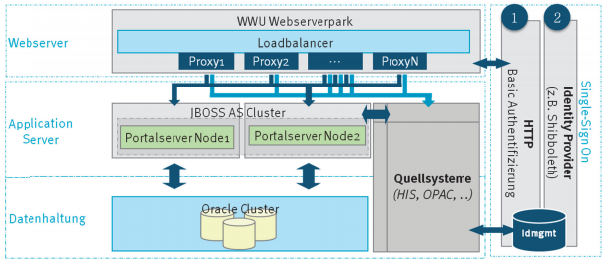
\includegraphics[width=\textwidth]{kapitel/gruppe3/bilder/struktur_mywwu}
	\caption{technische Struktur des Portals myWWU der Universität Münster}
	\label{fig_struktur_mywwu}
\end{figure}
\newpage

\subsubsection{Integrierte Gesamtsuche}
\label{subsubsection_integrierte_gesamtsuche}
Wissenschaftliche Informationen sind häufig in verschiedenen Systemen angesiedelt. Durch die Einführung eines Systems zur integrierten Gesamtsuche würde die Suche an zentraler Stelle ausgeführt. Einzelne Systeme werden von den Suchenden nicht vergessen und die Integration neuer wissenschaftlicher Informationssysteme wird dauerhaft kommuniziert statt einmalig, wie es beispielsweise beim 
Versand einer Info-E-Mail der Fall wäre.

Die WWU Münster nutzt dafür einen „Suchmaschinen-basierte[n] Ansatz auf Basis der Software Primo von der Firma Ex Libris“.\footcite[Vgl.][41]{vogl_fortschritte_2012} Dafür nötig ist eine Normalisierung der Datenformate interner und externer Quellen, welche „insbesondere auf der Detailebene […] aufwändige Anpassungen und Eigenentwicklungen notwendig“ machen.\footcite[Vgl.][42]{vogl_fortschritte_2012}

Quellsysteme, ausgehend von diesem Konzept, können sein:
\begin{itemize}
	\item Alfresco
	\item Identity Management System
	\item ForschungsDB Niedersachsen
	\item moodle
	\item Open Journal System
	\item Hochschulexterne Informationssysteme wie zum Beispiel video2brain
	\item ggf. Bibliothekssuche
\end{itemize}

Wichtig ist neben korrekten und vollständigen Ergebnissen auch die Benutzbarkeit. Bekannte Funktionalitäten aus anderen Suchmaschinen, wie Gruppierungen, sollten integriert sein, wie auch eine übersichtliche und funktionale Benutzeroberfläche.\footcite[Vgl.][43]{vogl_fortschritte_2012}

\subsection{Ausblick bei Integration der Bibliothek}
Auch wenn die Bibliothek in dieser Ausarbeitung ausgenommen ist, muss erwähnt werden, dass bei Informationsmanagement-Projekten anderer Hochschulen und Universitäten auch die Bibliotheken integriert werden. Die über die Bibliothek zur Verfügung gestellten Informationen werden vor allem für Forschung und Lehre genutzt, welches die Kernaufgaben von Hochschulen sind.

Dementsprechend kann die Integration der Bibliothekssuche in die integrierte Gesamtsuche zur Aufwertung der Suchergebnissen beitragen. Um auch nicht digital verfügbare bzw. archivierte Zeitschriften und Bücher integrieren zu können, kann ein Digitalisierungssystem eingeführt werden. Die WWU Münster setzt dafür vor Ort frei verfügbare Scanner zuzüglich der Software scantoweb ein.\footcite[Vgl.][50]{vogl_fortschritte_2012}

\section{Abwägung des Einsatzes eines Informationsmanagers an der Hochschule Emden/Leer - JL}
\label{section_einsatz_cio}
\textit{Autor: Julia Lübke}

Das Soll-Konzept analysiert die Ist-Situation um den derweilen Zustand der  Hochschule Emden/Leer zu ermitteln. Daraus lässt sich erkennen, ob es generell einer Verbesserung des Informationsmanagements in der Zukunft bedarf und wo diese anzusetzen sind oder ob noch kein Informationsmanagement besteht und aufgebaut werden muss. Dazu sind verschiedene Aspekte zu beleuchten. Neben der Anforderung des zukünftigen Marketings, den technischen Neuerungen und der darauf folgenden Umsetzung ist zu klären, ob die Hochschule Emden/Leer eine Führung im Bereich des strategischen und operativen Informationsmanagements benötigt.

Im klassischen Informationsmanagement ist dies die Aufgabe eines Informationsmanager, dem sogenannten Chief Information Officer. Wie auf der Abbildung \ref{fig_def_inm} zu erkennen, arbeitet der Informationsmanager dabei als zentrale Schnittstelle zwischen technischen, organisatorischen und wirtschaftlichen Teilbereichen und dient dort als sogenannter Mittler zwischen den verschiedenen Bereichen und untersucht dabei die Informations- und Kommunikationstechniken in allen unterschiedlichen Bereichen um diese sinnvoll einzusetzen. 
\footcite[86]{definition_informationsmanager}

\begin{figure}[h!]
	\centering
	\includegraphics[width=10cm]{kapitel/gruppe3/bilder/definition_informationsmanager}
	\caption{Definition Informationsmanager}
	\label{fig_def_inm}
\end{figure}

\subsection{Analyse des Ist-Zustandes}
\label{subsection_analyse_ist_zustand}

Bezug nehmend auf das Organigramm aus Abbildung \ref{fig_organigramm_HS} der Hochschule Emden/Leer und der Bewertung aus  \ref{bewertung_gewichtung} ist festzuhalten, dass der Hochschule kein klassisches Informationsmanagement zugrunde liegt, sondern ein zentrales Informationssystem. Es werden bereits Informationen verwaltet und weitergegeben, jedoch nicht an zentraler Stelle. Zentrale Systeme, siehe Abbildung \ref{fig_zentrale_systeme}, Kapitel \ref{section_zustaendigkeiten}, sowie unterschiedliche Möglichkeiten werden für alle zur Verfügung gestellt und in Anspruch genommen. 

Es gibt keine Verwaltung, sondern verschiedene Bereiche, die unterteilt sind in Arbeitsgruppen, Abteilungen sowie Rechenstelle und Pressestelle. Weiterhin beinhaltet das Informationssystem verschiedene Prozesse zum Datenaustausch bzw. Datenfluss und Back-up-Transfer aus verschiedenen Systemen.  Die Nutzung des gegenwärtigen Informationssystems wird unterschiedlich stark genutzt oder ausgelastet. 

Von den zentralen Einrichtungen nehmen das Hochschulrechenzentrum und die Bibliothek einen wichtigen Platz in der Hochschule Emden/Leer ein. Das Hochschulrechenzentrum übernimmt derweil viele Aufgaben der Informationsverwaltung und Planung. Doch nicht nur da werden Informationen gesammelt und ausgewertet. Die Hochschule in Emden definiert eine ganze Reihe von Arbeitsgruppen, beispielsweise die Arbeitsgruppe Zahlen, Daten, Fakten, die Kennzahlen der Hochschule und der einzelnen Fachbereiche sammelt und diese auswertet und an gewünschte Stellen weitergibt.  

Aktuell besteht keine erweiterte Vernetzung unterschiedlicher Intranetzsysteme zwischen verschiedenen Hochschulen. Lediglich im Bereich der Bibliothek werden Inhalte an mehreren Standorten gemeinsam genutzt. Abschließend ist zu erwähnen, dass die Hochschule Emden/Leer auch keine Einzelperson oder ein Gremium als zentrale Informationsverwaltung nutzt.


\subsection{Betrachtung des zu erwartenden Soll-Zustandes }
\label{subsection_betrachtung_soll}

Nach Betrachtung der Best-Practice-Beispiele aus Kapitel \ref{chapter_best_practice_beispiele} lässt sich erkennen, dass jede Hochschule und auch Universität den Umgang des Informationsmanagements anders angeht. So spielen verschiedene Faktoren eine Rolle, die an jeder Hochschule/Universität unterschiedlich ausgelegt sind. Ein Vergleich der betrachteten Universitäten mit der Hochschule Emden/Leer zeigt, dass Emden eine wesentlich kleinere Institution ist und somit andere Ansprüche hat und weniger komplexe Strukturen besitzt, als beispielsweise die WWU Münster, die über 40.000 Studierende pflegt. 

Trotz unterschiedlich integrierter Möglichkeiten der unterschiedlichen Universitäten zur Umsetzung des jeweiligen Informationsmanagements, gibt es doch Bereiche, die gleich oder zumindest ähnlich sind. So sind Bibliotheken, Gremien, Ausschüsse, ebenso wie Fachbereiche, das Rechenzentrum und auch das Präsidium Teil einer jeden Hochschule oder Universität. 

Es ist also zu schauen, wo sich das Informationsmanagement als zentrale Informationsquelle ansetzen lässt, um mehrere Bereiche und Bestandteile untereinander zu verbinden. Fakt ist, dass es in Emden bereits drei Arbeitsgruppen gibt, die bestimmte Informationen gewinnen und filtern.  So wäre zu betrachten, wie die Zentralisierung einer übergeordneten Informationsquelle und -weitergabe zu bewerkstelligen wäre und wie der Aufbau einer neuen Struktur die Möglichkeit zur Verbesserung des Informationsaustausches aussehen könnte. 

In Kapitel \ref{subsection_zentralisierung_integration} wird beschrieben, dass die meisten Hochschulen und Universitäten unter einer neu geschaffenen Organisation arbeiten. Dabei spielen das Rechenzentrum, die Bibliothek und die Verwaltung immer eine Rolle in einer solchen Organisation. Kein Konzept ist maßgeschneidert und nicht auf jede Hochschule oder Universität anwendbar.

\subsubsection{Empfehlungen der ZKI bezüglich des Informationsmanagers}
\label{subsubsection_zki}

Neben den verschiedenen Projekten und Einrichtungen, die im Kapitel \ref{chapter_best_practice_beispiele} beleuchtet werden, und aufzeigen, wie mit dem Informationsmanagement umgegangen wird, gibt es noch die Zentren für Kommunikation und Informationsverarbeitung (ZKI) in Lehre und Forschung, die Empfehlungen für Hochschulen bezüglich des Informationsmanagements und besonders Empfehlungen für den Informationsmanager aussprechen.

Blickend auf die Publikation der ZKI basierend auf einer Studie der CIOs und IT-Governance an deutschen Hochschulen aus dem Jahre 2014 wurden über mehrere Jahre von der Kommission für IT-Infrastruktur der Deutschen Forschungsgemeinschaft (KfR) hinweg folgende Empfehlungen für Hochschulen ausgesprochen.

Zwischen 2001 - 2005 gab die KfR folgende Empfehlung:

\textit{" Aufgrund der Relevanz der Informationsverarbeitung für alle Bereiche der  Hochschule wird empfohlen, 
	einen Generalverantwortlichen für Information und  Kommunikation (CIO, Chief Information Officer) 
	in der Hochschulleitung oder ein geeignetes Leitungsgremium mit entsprechenden 
	Entscheidungskompetenzen mit der Entwicklung und  Koordinierung aller IuK-Aufgaben 
	zu betrauen."}\footcite[3]{zki_studie_cio_2014}

Zwischen 2006 - 2010 werden weitere Ausführungen genannt:

\textit{" Integriertes Informationsmanagement ist daher zur wesentlichen Aufgabe bei der Planung des 
	Einsatzes moderner Techniken von Information und Kommunikation für die Hochschulen geworden. 
	Eine solche Planung setzt die Position eines Verantwortlichen für Information und Kommunikation 
	als Mitglied der Hochschulleitung (CIO: Chief Information Officer) voraus, wie er in der Wirtschaft 
	und an verschiedenen Hochschulen bereits etabliert ist."}\footcite[16]{zki_studie_cio_2014}

Die KfR Empfehlungen zwischen 2011-2015 werden noch weiter ausgebaut:

\textit{"In der Hochschulpraxis lassen sich vier unterschiedliche Umsetzungstypen beobachten:  Strategischer CIO mit Leitungsfunktion: Ein Vizepräsident - oder eine Vizepräsidentin - ist explizit für das Informationsmanagement zuständig. Teilweise übernimmt auch der Kanzler die Zuständigkeit für das Informationsmanagement.}

\begin{itemize}
	\item \textit{Strategischer CIO mit Stabsfunktion: Ein Hochschullehrer oder IT-Manager - 
		bzw. Hochschullehrerin/IT-Managerin - im Präsidialstab koordiniert das Informationsmanagement.} 
	\item \textit{Operativer CIO: Der Leiter - bzw. die Leiterin - einer zentralen 
		Informationsinfrastruktureinrichtung fungiert gleichzeitig als CIO der Hochschule.}
	\item \textit{Kollektiver CIO: Die CIO-Funktion wird von einem Lenkungsausschuss mit zwei bis 
		drei Personen ausgeübt, der allerdings - anders als die traditionelle Senatskommission - über 
		unmittelbare Entscheidungsbefugnisse verfügt.}
\end{itemize}
\textit{Jede dieser CIO-Umsetzungsvarianten hat ihre Vor- und Nachteile. Es hängt von den 
	Gegebenheiten an den Hochschulen und insbesondere auch von Personen ab, welche 
	Umsetzung die am besten geeignete ist. Wichtig ist, dass der CIO - in welcher Form 
	auch immer - einen unmittelbaren Zugang zur Hochschulleitung hat und die IT-Belange 
	der gesamten Hochschule strategisch - mit unmittelbarer Richtlinien- und 
	Entscheidungskompetenz - fährt und verantwortet."} \footcite[17]{zki_studie_cio_2014}

Abschließend ist zu sagen, dass die ZKI/KfR einer Hochschule eine zentrale Informationsschnittstelle in Form eines CIOs oder eines CIO-Gremiums empfiehlt.

\subsubsection{Informationsmanager oder Gremium als zentrale Informationsschnittstelle}
\label{subsubsection_cio_gremium}

Der Aufbau eines Informationsmanagements bedarf vieler Schritte und Überlegungen (siehe Abschnitt \ref{begriffsdefinition_inm}). Neben den Veränderungen und deren Umsetzung ist zu klären, ob der bisherige Austausch der Informationen der Hochschule Emden/Leer durch eine zentrale Einrichtung oder einer Einzelperson und entsprechenden Verantwortlichkeiten geregelt werden soll. Um dies in ein reales Szenario zu bekommen, sind die Möglichkeiten aufzuzeigen und ein entsprechend passendes Modell für die Hochschule Emden/Leer zu entwickeln. Dazu werden in Kapitel  \ref{chapter_best_practice_beispiele}, ebenso wie in der Studie der ZKI verschiedene Konzepte des Chief Information Officers (CIO) aufgezeigt. 

Ein einheitliches Konzept ist nicht gegeben, sodass nicht jede Lösung auch passend für die Hochschule Emden/Leer ist. Die betrachteten Universitäten haben ein anderes Anforderungsprofil an ein Informationsmanagement und deren zentrale Leitung als Emden, die wesentlich kleinere und weniger komplexe Strukturen besitzt. Zu den betrachteten Best-Practice-Beispielen lassen sich zusätzlich die Empfehlungen der KfR heranziehen. 

Alle haben gemeinsam, dass das Verwalten der Informationen aus einer Schnittstelle heraus geschieht. Auch dieses Konzept ist für die Hochschule Emden/Leer zu überlegen. Nun stellt sich die Frage, wo diese Schnittstelle anzusetzen ist und wer die Aufgaben übernehmen soll. Verschiedene Möglichkeiten sind hier zu betrachten. Zum einen gibt es das Personenmodell, den CIO, beschrieben in \ref{anforderungsprofil_informationsmanager} und \ref{eingliederung_informationsmanager} der die Schnittstelle bildet, zum anderen gibt es die Möglichkeit eines CIO-Gremiums. 


\textbf{Personenmodell:\newline}
Eine Person wird als Informationsmanager herangezogen und übernimmt die in den Abschnitten \ref{aufgaben_funktionen_informationsmanager},\ref{anforderungsprofil_informationsmanager} und \ref{eingliederung_informationsmanager} angegebenen Aufgaben, die hochschulangepasst sind. Dabei ist zu betrachten, wer diese Aufgabe übernehmen soll. Der CIO kann aus der Privatwirtschaft geordert werden. Dabei ist zu bedenken, dass dafür eine Menge Ressourcen benötigt werden. Neben dem aufwendigen Bewerbungsprozess und der Einstellung erfolgt die Einarbeitungszeit und die Einführung des Informationsmanagements durch den CIO. Als weiterer Punkt sind noch die erhöhten Personalkosten in dieser Zeit zu nennen.

Neben der Möglichkeit einen CIO aus der Privatwirtschaft zu holen, besteht auch die Möglichkeit einen hochschulinternen Mitarbeiter zu involvieren. Der Bewerbungszeitraum und die Einarbeitung verringern sich, da ein bestehender Mitarbeiter die Hierarchie und die Arbeitsweise der Hochschule Emden/Leer bereits versteht und kennt. Allerdings ist nicht zu verachten, dass diese Person, entweder eine Mehrbelastung durch die zusätzlichen Aufgaben des Informationsmanagers tragen muss oder für die vorherige Stelle ein neuer Mitarbeiter gesucht werden müsste, was auch in diesem Fall mit einem erhöhten Kosten- und Zeitaufwand verbunden wäre.


\textbf{Gremiummodell:\newline }
Soll das Informationsmanagement allerdings nicht nur von einer einzelnen Person betrieben werden, ist zu klären, wer diese Aufgabe übernehmen soll. Dazu ist immer in Vergleich zu setzen, welche Parameter greifen. Die Studie der ZKI besagt, Bezug nehmend auf die Abbildung \ref{fig_herkunft_cio_hochschulen}, dass die Gremienmitglieder aus ganz unterschiedlichen Bereichen der Hochschule kommen. Ist dies der Fall und ein Gremium wird ernannt, ist ein Arbeitsaufwand der anfallenden CIO Tätigkeiten auf alle Mitglieder aufgeteilt. So ist der Gesamtaufwand pro Person prozentual geringer als bei einer einzelnen Person, die mindestens 50\% ihrer Zeit in CIO-Aufgaben investiert. 



\begin{figure}[h!]
	\centering
	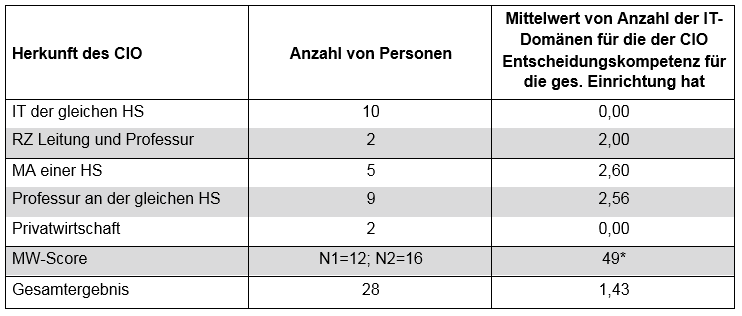
\includegraphics[width=\textwidth]
	{kapitel/gruppe3/bilder/herkunft_cio_hochschulen}
	\caption{Herkunft des CIO an verschiedenen Hochschulen, nach ZKI CIO-Studie}
	\label{fig_herkunft_cio_hochschulen}\footnote{\cite[8]{zki_studie_cio_2014}}
\end{figure}



\subsection{Empfehlung für die Hochschule Emden/Leer}
\label{empfehlung_cio}

Durch stetig wachsende Anforderungen besonders im Bereich der technischen Neuerungen und deren Umsetzung sowie Weitergabe und Verarbeitung von Informationen spricht die KfR seit Jahren Empfehlungen bezüglich eines Informationsmanagers an Hochschulen aus. Durch zusätzliches Betrachten der Best-Practice-Beispiele wird gezeigt, dass jede Hochschule andere Anforderungen besitzt und bezüglich ihrer Größe, Lage und Ansprüche anders mit einem Informationsmanagement umgeht, jedoch alle gemeinsam haben, dass eine zentrale Schnittstelle gebildet wird, die zusammenlaufende Informationen verarbeitet, auswertet und weitergibt. 

Nicht jede Lösung eignet sich dabei für jede Hochschule. In einer Studie der ZKI geht dies ebenfalls hervor. Die Studie befasst sich mit dem Informationsmanager und spricht dabei Empfehlungen für Hochschulen aus. Dabei ist festzuhalten, dass es neben dem Einzelpersonen-Modell auch ein CIO-Gremium-Model geben kann, je nach Bedürfnis der Hochschule. Eine Einzelperson kann hierbei vorteilhafter sein als ein Gremium, dennoch ist zu betrachten, dass ein enormer personeller Kosten- und Zeitfaktor entstehen wird, da nicht zu verachten ist, dass das Aufbauen einer solchen Struktur Jahre in Anspruch nimmt. Es ist daher abzuwägen, ob sich dieser finanzielle Aufwand für die Hochschule Emden/Leer lohnt. 

Da Emden bereits die drei Arbeitsgruppen Zahlen, Daten und Fakten, Web und Moodle besitzt, detaillierter beschrieben in \ref{subsection_arbeitsgruppen_informationsaustausch}, die wichtige Informationen sammeln und verarbeiten, wäre der Hochschule Emden/Leer eine Empfehlung zu einem CIO-Gremium auszusprechen. Durch die bereits existierenden Arbeitsgruppen ist aus jedem Bereich bereits ein Vertreter vorhanden. 

Die Hochschule Emden/Leer ist diesbezüglich schon gut aufgestellt, um weitere Schritte beim Einführen dieses Konzeptes einleiten zu können. Die anfallenden Aufgaben werden auf das gesamte  Gremium aufgeteilt, sodass eine geringere Mehrbelastung entsteht. Abb. \ref{fig_moegliches_gremium} zeigt die Umstellung des Organigramms der Hochschule Emden/Leer, als mögliche Organisation. Das Gremium unterliegt dabei der Hochschulleitung. Da das Rechenzentrum bereits wichtige und zentrale Aufgaben besonders im technischen Bereich übernimmt, wäre es sinnvoll das Gremium aus dem Bereich heraus zu gründen. 

\begin{figure}[h!]
	\centering
	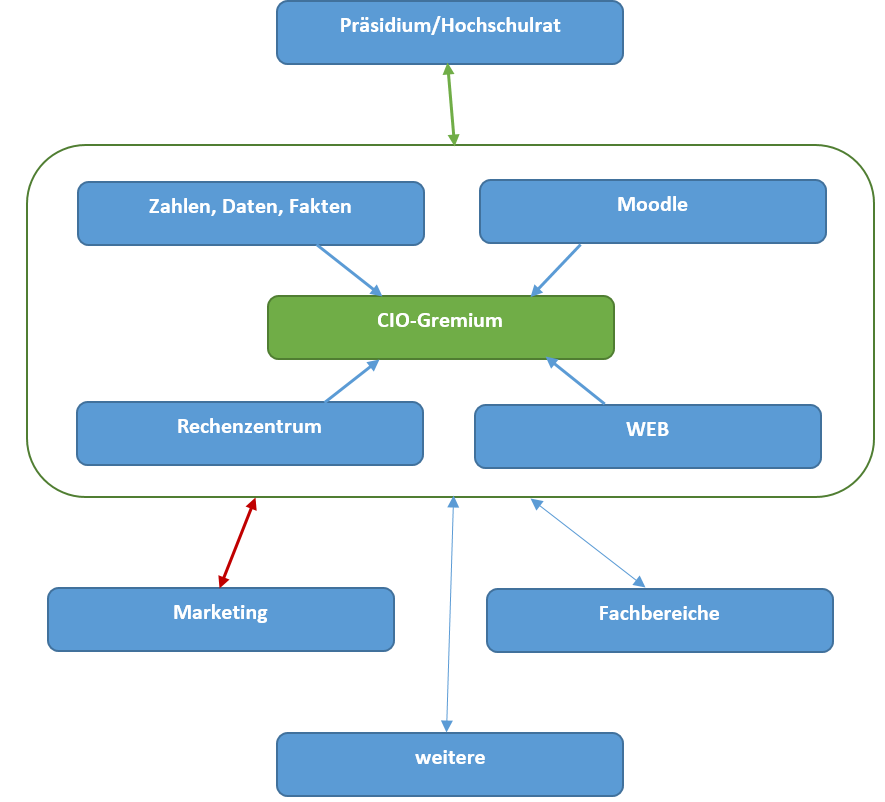
\includegraphics[width=\textwidth]
	{kapitel/gruppe3/bilder/moegliches_cio_gremium}
	\caption{Umstellung/Änderung des Organigramms der Hochschule Emden 	hinsichtlich eines CIO Gremiums}	
	\label{fig_moegliches_gremium}
\end{figure}

In Verbindung mit den drei bereits existierenden Arbeitsgruppen würde sich eine Mischform zwischen strategischem und kollektivem CIO für die Hochschule Emden/Leer anbieten. Das bietet die Möglichkeit sich den gegenebheien der Hochschule anzupassen und ein auf Emden/Leer awäre, dass das CIO-Gremium eng mit dem Marketing zusammenarbeitet und somit von der vorgestellten Möglichkeit Feedback zu sammeln, beschrieben in \ref{feedback} profitieren würde. So können anfallende Probleme direkt diskutiert und Lösungen gefunden werden. 




%\chapter{Umsetzungsplanung: Change Management und Migration - MB, CH}

\textit{Autoren: Marco Beckmann, Christian Halfmann}

Im Folgenden soll im Rahmen der Umsetzungsplanung erläutert werden, wie zum  einen Veränderungen unter Berücksichtigung der Betroffenen mittels Change Management initiiert und durchgeführt werden können, und wie zum anderen mittels geeigneter Migrationskonzepte die technische Umsetzung realisiert werden kann.

\section{Umsetzungsplanung - CH}
\todo[inline]{CH: Einleitungssatz schreiben}

\subsection{Positionsbestimmung}
Für einen erfolgreichen Umsetzungsplan mit der Zielsetzung einer Neuordnung des Informationsmanagements an einer Hochschule ist eine Positionsbestimmung der aktuellen Situation von elementarer Bedeutung. Hierzu muss der Ist-Zustand des aktuellen Informationsmanagements mit der Zielformulierung des avisierten Informationsmanagements an der Hochschule erfasst und abgeglichen werden. 

Da solche Veränderungen in der Regel einen langwierigen Prozess darstellen, ist es ratsam, Prioritäten zu definieren und die einzelnen Teilbereiche anhand der Dringlichkeit umzusetzen.

Ist die Position bestimmt, kann davon ausgehend ein entsprechender Migrationsplan (vgl. Kapitel \ref{section_migrationskonzepte}) und, wenn noch nicht geschehen, ein Changeplan (vgl. Kapitel \ref{subsection_change_management}) erstellt werden. Je nach Art und Umfang der Veränderungen sollte allerdings das Change Management nicht erst nach der Positionsbestimmung angewandt werden, sondern schon bei der Zielbestimmung – also mit in die Erarbeitung des möglichen Soll-Zustands einfliessen.

Diese Ausarbeitung wird sich aus Gründen der Komplexität im praxisbezogenen Teil nicht auf das gesamte Informationsmanagement der Hochschule Emden/Leer beziehen können. Exemplarisch wird daher eine Umsetzungsplanung an den Beispielen des Dokumentenmanagements Alfresco und der Erstellung eines responsive Designs der Webpräsenz der Hochschule erarbeitet.

Alfresco wird derzeit noch nicht an der Hochschule eingesetzt. Zur Zeit werden Dokumente in verschieden Systemen verwaltet und zugäglich gemacht. Für die Webpräsenz wird derzeit ein TYPO3-System in der Version 4.5 LTS (Long Term Support) genutzt, welches noch nicht für mobile Endgeräte optimiert ist.

\subsection{Change Management}
\label{subsection_change_management}

\todo[inline]{CH: Einleitungssatz schreiben}

\subsubsection{Grundlagen des Change Managements}
Die Umsetzung einer Neuordnung des Informationsmanagements an einer Hochschule bedeutet auch Wandel und Veränderungen. Um das optimal zu steuern, bedarf es spezieller Managementtechniken, welche sich unter dem Begriff Change Management zusammenfassen lassen. Im Vordergrund aller Betrachtungen steht der Faktor Mensch, denn für eine erfolgreiche Umsetzung von Veränderungen ist die aktive Unterstützung der Betroffenen von erheblicher Bedeutung.\footcite{lauer_change_2014}

\begin{figure}[h!]
	\centering
	\includegraphics[width=10cm]{kapitel/gruppe4_1/bilder/drei_phasen_modell}
	\caption{3-Phasen-Modell nach Kurt Lewin}
	\label{fig_drei_phasen_modell}
\end{figure}

\begin{itemize}
	\item Die Betroffenen sollen Veränderungen motiviert werden.
	\item Die Betroffenen sollen für Veränderungen trainiert werden und der Veränderungsprozess vollzogen werden.
	\item Die die Veränderungen sollen Stabilisiert werden.
\end{itemize}


Nach Thomas Lauer sollte das Change Management grundsätzlich an drei Punkten ansetzen:
\begin{itemize}
	\item \textbf{Individuum:} Das Individuum beschreibt jeden Einzelnen. Ohne die Mitarbeit der Betroffenen ist ein Wandel unmöglich. Das Change Management soll nicht nur die Fähigkeiten des Einzelnen an neue Herausforderungen anpassen, sondern auch die positive Einstellung gegenüber der Ziele des Wandels aller Betroffenen fördern.
	\item \textbf{Unternehmensstruktur (bzw. Hochschulstruktur):} Die Unternehmensstruktur umfasst Aufbau- und Ablauforganisation sowie Strategien und Ressourcen. Veränderungen in diesen Bereichen sind auf dem Papier grundsätzlich einfach.
	\item \textbf{Unternehmenskultur (bzw. Hochschulkultur):} Die Unternehmenskultur beschreibt dauerhafte, über lange Zeit gewachsene Strukturen die für Einstellung, Werte und Regeln des Umgangs verantwortlich sind. 
\end{itemize}

In den meisten Fällen bringt ein Wandel in den oben genannten Bereichen Veränderungen in allen Dimensionen mit sich, die sich wechselseitig beeinflussen.\footcite{fisch_veraenderungen_2008} 

So ist z. B. ein Wandel ohne die Einbeziehung der Unternehmenskultur oftmals zum scheitern verurteilt.\footcite{lauer_change_2014} Das heißt, für ein erfolgreiches Change Management sollten grundsätzlich die Abhängigkeiten der Bereiche untereinander berücksichtigt werden.

Veränderungen bedeuten Neues und Ungewohntes für alle Betroffenen. 
Betroffene müssen veränderte Aufgaben erledigen, neue Technologien und Methoden erlernen, erneut soziale Beziehungen zu Kollegen, Vorgesetzten oder Kunden aufbauen, mit Problemen in der Implementierungsphase umgehen und ggf. ihre Werte in Einklang mit neuen Standards und Zielen der Organisation bringen.\footcite{fisch_veraenderungen_2008}

Dies kann zu Zweifeln und Widerständen führen, was im schlimmsten Fall ein Scheitern des gesamten Vorhabens bedeuten kann. Als Ursache eines gescheiterten Wandels steht der Widerstand an oberster Stelle. Mangelhafte Prozessteuerung, zu schnelles Veränderungstempo und unklare Zielsetzungen spielen dabei ein wichtige Rolle und können Gründe für eben diesen Widerstand sein.\footcite{lauer_change_2014}

Die Bereitschaft zum Wandel nimmt zu, wenn die Betroffenen überzeugt sind, das die Veränderungen ihnen persönlich nutzen, ihre Identität nicht bedroht ist und ihre Werte und Ziele mit dem Wandel in Einklang gebracht werden können.

Des weiteren wird die Bereitschaft zum Wandel gefördert wenn die Betroffenen über Fähigkeiten verfügen, die den veränderten Anforderungen gerecht werden. Die Aufgabe des Change Management ist es, durch Information, Partizipation, Unterstützung (z. B. Coaching) und Anreizgestaltung den Betroffenen die Zweifel und Unsicherheit zu nehmen.\footcite{fisch_veraenderungen_2008}

\begin{itemize}
\item \textbf{Kommunikation}
Nach Thomas Lauer ist einer der entscheidendsten Erfolgsfaktoren des Change Managements die Kommunikation. Kommunikation schafft Transparenz und damit Orientierung und dient damit auch der Beilegung von Widerständen. Damit ist aber auch ein potenzieller Misserfolg eines Change Managements auf die Kommunikation zurückzuführen. Fehlinterpretationen und Missverständnisse können schnell zu Konflikten führen.\footcite{lauer_change_2014}

Es sollten also entsprechende Kommunikationsstrategien und Kommunikationspläne erarbeitet werden, um die Betroffenen für die Veränderungen zu gewinnen und Missverständnissen aus dem Weg zu gehen. In der Startphase sollten die Betroffenen über Gründe, Ziele, Notwendigkeit, Nutzen und den zeitlichen Ablauf informiert werden. Aber auch potentielle Risiken und Schwierigkeiten sollten von Anfang an offen kommuniziert werden.\footcite{fisch_veraenderungen_2008}

In der Durchführungsphase ist es wichtig die Kommunikation aufrecht zu erhalten. Beispielsweise können Projektfortschritte regelmäßig an alle Betroffenen weitergegeben werden. Durch das Aufrechterhalten der Kommunikation können frühzeitig Widerstände erkannt und überwunden werden.\footcite{lauer_change_2014}

\item \textbf{Partizipation}
Ein weiterer wichtiger Erfolgsfaktor ist die Partizipation. Das Einbinden möglichst vieler Betroffenen in den Change Prozess erhöht die Motivation und hilft den Betroffenen sich mit den Veränderungen zu identifizieren. Haben Betroffene andere Positionen oder Sichtweisen gegenüber des Wandels als die Organisation müssen diese Widerstände nicht gleich negativ ausgelegt werden. Die Ideen und Vorschläge der Betroffenen können in den Change Prozess einfliessen und weiterhin Veränderungen optimieren.

\item \textbf{Unterstützung}:
Besonders wenn es um neue Technologien, Werkzeuge oder Verfahren geht, ist Unterstützung für die Betroffenen gefordert. Die Unterstützung hat zum Ziel, die Betroffenen des Wandels auf die zusätzlichen oder neuen Anforderungen vorzubereiten. In den Meisten Fällen geschieht das in Form von Weiterbildung oder Coaching.

Des weiteren fördert eine vom Unternehmen ausgehende Weiterbildung nicht nur den Aufbau von Qualifikationen und die Erweiterung des Wissens der Betroffenen, sondern auch die Motivation. Den Betroffenen wird das Gefühl gegeben, dass in sie investiert wird und damit auf eine langfristige Partnerschaft gesetzt wird.
\end{itemize}

In dem Sinne ist die Aufgabe des Change Managements also nicht die Definition von Zielen, es soll den Weg des gesamten Vorhabens vom Ausgangspunkt bis zum Ziel gestalten\footcite{lauer_change_2014} und den Betroffenen des Wandels ihre Zweifel nehmen.

Auch bei perfekt geplanten Change-Projekten können Widerstände nicht ausgeschlossen werden. Das Change Management sollte in der Lage sein auf diese Widerstände zu reagieren. Sollte sich in dem laufenden Change Prozess herausstellen, dass bestimmte Bedingungen nicht mehr aktuell sind, sollten Ziele und Veränderungen angepasst und neu formuliert werden.\footcite{fisch_veraenderungen_2008}

Der Wandel kann nur gelingen wenn die Betroffenen hinter den Plänen stehen und die Veränderungen unterstützen. Im Fall der Hochschule treten einige Besonderheiten auf, auf welche im nächsten Kapitel genauer eingegangen wird.

\subsubsection{Change Management an Hochschulen}
\label{subsubsection_change_management_an_HS}
Im vorherigen Kapitel wurden die Adressaten des Change Managements als Betroffene betitelt. Diese sind im klassischen Fall Mitarbeiter eines Unternehmens, in dem Veränderungen vorangetrieben werden sollen. Diese Mitarbeiter sind  meist Bestandteil einer klaren Hierarchie, an dessen oberster Stelle das Management steht, von welchem der Wandel initiiert wird. 

Im speziellen Fall von Hochschulen setzen sich die Betroffenen aus Professoren, wissenschaftlichen Mitarbeitern, Verwaltungsmitarbeitern und Studierenden zusammen, welche autonome Endscheidungen treffen. Studenten entscheiden, was sie lernen, Dozenten entscheiden welche Inhalte sie lehren.\footnote{\cite{hoelscher_wissenschaft_2011}}

Hinzu kommen Fakultäten, Fachbereiche und Institute, welche sich selbst organisieren und nahezu autonom und unabhängig von einander agieren.\footnote{\cite{fisch_veraenderungen_2008}} 
Dies erschwert die Kommunikation untereinander sowie das Erschaffen von Synergien und das Entwickeln übergeordneter Ziele und Strategien.

Ein erfolgreiches Change Management muss also die besonderen Gegebenheiten der Organisation Hochschule bei der Gestaltung und Auswahl entsprechender Maßnahmen berücksichtigen und auf sie eingehen.

Hierzu sollten die Betroffenen innerhalb der Hochschule frühzeitig in die Zielformulierung von Change Prozessen eingebunden werden. So kann Raum für Diskussionen geschaffen werden, denn die unterschiedlichen Bereiche der Hochschule vertreten oft unterschiedliche Interessen was zur Verschleppung oder Verzögerungen von Entscheidungen führen kann. In solchen Fällen kann ein Austausch mit externen Experten oder internen Stäben helfen, Entscheidungen voranzutreiben.\footnote{\cite{fisch_veraenderungen_2008}}

Studien zu Change Management an Hochschulen haben herausgefunden, dass auch hier Information und Partizipation wichtige Elemente des Change Managements sind:
\begin{itemize}
	\item Eine Studie zur Evaluation der Strategieumsetzung an der Universität Heidelberg könnte belegen, dass Partizipation und die Qualität der Information positive Auswirkungen gegenüber Veränderungen bei den wissenschaftlichen Mitarbeitern und Studierenden hatte. Je besser die Betroffenen über die Ziele der Veränderungen informiert wurden und desto mehr eigene Ideen sie in die Veränderungen einbringen konnten, desto eher wurde der Wandel positiv bewertet und die Bereitschaft gesteigert, aktiv an der Umsetzung mitzuwirken.\footnote{Quelle fehlt noch immer}
	
	\item Bei Veränderung des Curriculums und der Einführung neuer Prozesse und Strukturen des Qualitätsmanagements an einem amerikanischen Collage zeigte sich, dass es nicht nur darum geht, Partizipation zu erhöhen, sondern auch darum, Lehrende so anzuleiten, dass Entscheidungen nicht zu autoritär getroffen werden, noch durch zu starke Gleichberechtigung in die Länge gezogen oder gar verhindert werden.\footnote{\cite{cohen_major_2005}}
	
	\item Eine weitere Studie zur Implementierung von E-Learning konnte belegen, dass integratives Change Management erforderlich ist, um Veränderungen nachhaltig zu implementieren. Wurden Maßnahmen wie z. B. Training, Beratung oder didaktische Szenarien aufeinander abgestimmt, wirkt sich das positiv auf die Nutzung von E-Learning aus.\footnote{\cite{fuchs_change_2007}} 
\end{itemize}

Aus den Studien wird ersichtlich, dass Information und Partizipation wichtige Element des Change Managements darstellen. Aber auch Schulungen, Trainings, oder Coaching spielen eine große Rolle. Allerdings kann es zur Herausforderung werden, potenzielle Teilnehmer für Weiterbildungen aus dem Kreise der Professoren oder der Hochschulführung zu gewinnen, da diese auf ihrem Fachgebiet als Experten gelten und eine Teilnahme an solchen Weiterbildungsangeboten als Ausdruck persönlicher Defizite werten könnten. Dennoch bietet es sich an, bei komplexen Veränderungen zusätzliche Kompetenzen durch Training oder Coaching zu erschließen.\footnote{\cite{fisch_veraenderungen_2008}}

Durch die besonderen Strukturen und Gegebenheiten einer Hochschule, muss  ein potentielles Change Management möglichst sensibel agieren und alle relevanten Akteure informieren und partizipieren lassen, um am Ende auch den gewünschten Erfolg und somit die avisierten Ziele zu erreichen.

\subsubsection{Changeplan}
Wie Eingangs erwähnt, kann hier nicht auf das gesamte Informationsmanagement der Hochschule eingegangen werden. Daher wird der Changeplan sich exemplarisch auf die Beispiele Alfresco und Responsive Design beziehen, wobei es sich in beiden Fällen um Veränderungsprozesse im IT-Bereich handelt.

Der Changeplan soll unter Betrachtung der beschrieben Grundlagen des Change Managements sowie der besonderen Rahmenbedingungen an Hochschulen erstellt werden.

Hinzu kommt, dass es sich hier um Veränderungsprozesse im IT-Bereich handelt. 
Hier gibt es in der Praxis zwei Herangehensweisen an das Change Management. 
Zum einen die deterministische Sichtweise, welche Technik als Ausgangspunkt für alle Veränderungen und Gestaltungsmaßnahmen sieht, und zum anderen die sozio-technische Sichtweise, welche technisches und soziales gemeinsam optimiert1 \footnote{\cite{feldmuller_change_2007}}

In dem besonderen Fall einer Hochschule und deren Gegebenheiten, sollte die sozio-technische Herangehensweise der deterministischen vorgezogen werden (vgl. Kapitel \ref{subsubsection_change_management_an_HS}).  

Angelehnt an die genutzten Change Management Tools welche zur Unterstützung der Strategieumsetzung an der Universität Heidelberg eingesetzt wurden, könnten die Tools für die Neuordnung des Informationsmanagements an der Hochschule Emden/Leer wie folgt aussehen.

\begin{table}
	\begin{tabularx}{\textwidth}{|X|X|X|X|}
		\hline \textbf{Veränderungs-prozesse steuern} & \textbf{Information und Kommunikation} & \textbf{Partizipation} & \textbf{Konsolidierung nach dem Go Live}\\
		\hline Definition einer Projektstruktur & Kommunikations-pläne & Feedback zur Optimierung der Veränderungspro-zesse & Support\\
		\hline Controlling durch Statusberichte & Informationsver-anstaltungen & Training / Coaching & \\
		\hline
	\end{tabularx}
	\caption{Change Management Tools}
	\label{tab_change_management_tools}
\end{table}

In wieweit und in welchem Umfang sich die einzelnen Bausteine für die Vorhaben Responsive Website und Alfresco Dokumentenmanagement einsetzen lassen, soll in den folgenden Kapitel näher betrachtet werden.

\paragraph{Responsive Website}\mbox{}\\ \\
Im Rahmen der Erstellung eines responsive Designs der Webpräsenz der Hochschule soll gleichzeitig eine aktuelle TYPO3 Version migriert werden.

Beide Vorhaben stellen eine technische Migrationen dar. Inhalte und Funktionen  der Webpräsenz werden von Veränderungen nicht betroffen sein. Lediglich im Layout, welches durch die responsive Implementierung für alle Medien optimal dargestellt wird, werden leichte Veränderungen wahrzunehmen sein.

Bei den Anwendern wird es dadurch keine Veränderungen bei Prozessen, Arbeitsweisen oder dem benötigtem Wissen geben. Daher ist auf psychologischer Ebene also kein umfangreiches Change Management von Nöten, da hier auch nicht mit Widerständen zu rechnen ist.

Jedoch bietet es sich an, bei einer Neu-Implementierung auch eventuelle Verbesserungen, sei es von Funktionen, Layout oder Usability, gleich mit zu implementieren. Dafür sollten alle relevanten Akteure (hier die Verantwortlichen der Internetauftritte der verschiedenen Bereiche) in das Vorhaben einbezogen werden und die Möglichkeit haben Vorschläge und Wüsche zu äußeren und über diese zu diskutieren.

Das eigentliche Change Management richtet sich in diesem Fall an die IT-Mitarbeiter welche die neuen Systeme aufsetzen und pflegen. Aber auch hier werden die Betroffen nicht vor neue Aufgaben, Prozesse oder Arbeitsweisen gestellt, da die Migration neuer Systeme im Aufgabenfeld eines IT-Mitarbeiters verankert ist.

\paragraph{Alfresco}\mbox{}\\ \\
Das Change Management für die Umstellung auf das Dateimanagement Alfresco ist dabei etwas Umfangreicher als bei der Erstellung eines responsive Designs für die Webpräsenz der Hochschule. 

Hier handelt sich um ein grundlegend neues System an der Hochschule. 
Daher sollten frühzeitig alle relevanten Akteure in den Endscheidungsprozess Einbezogen werden. 
Es empfiehlt sich einen Kommunikationsplan zu erstellen um schon frühzeitig eine Übersicht dafür zu bekommen wann welche Informationen an wenn und auf welchem Weg kommuniziert wird.

Im Sinne der Partizipation sollten alle relevanten Akteure die Möglichkeit haben während des Veränderungsprozess ihr Feedback zur Diskussion zu stellen. Diese Möglichkeit könnte beispielsweise auf einer Informationsveranstaltung, welche durch die Hochschulleitung organisiert wird, wahr genommen werden.

Hierbei können bei Bedarf weitere Anforderungen in das Lastenheft aufgenommen werden. Die Aufgabe des Managements ist es dabei zwischen den geforderten Anforderungen abzuwägen, sodass ein „Nein“ zu Änderungen oder Erweiterungen des Lastenhefts auch zielführend sein kann. Denn Entscheidungen auf dieser Ebene schaffen weitere Veränderungen für die Betroffenen.\footnote{\cite{kleinhesseling_change_2011}}

Nach Analyse aller Feedbacks und der Optimierung der Zielsetzung kann die Migration des neuen Systems (Alfresco) beginnen. Zur Erhöhung der Akzeptanz,  ist es nach wie vor wichtig auch in dieser Phase die Kommunikation, beispielsweise durch Statusberichte, mit den Betroffenen aufrecht zu erhalten.

Des Weiteren können Workshops und Weiterbildungen den Betroffen dabei helfen, ihre Zweifel weiter abzubauen und sich mit den neuen IT-System vertraut zu machen. Hierzu bietet Alfresco beispielsweise eigens entwickelte Trainings für Entwickler, Administratoren und End User an (vgl. Kapitel . \ref{subsubsection_migration_alfresco}).

Konnte durch das Change Management eine Vielzahl von Zweifeln und Vorbehalte der Betroffenen gegenüber der Veränderungen abgebaut werden, so treten die tatsächlichen Veränderungen erst nach der Migration und dem Go Live des neuen Systems in vollem Umfang in Kraft. In dieser Phase muss die gewonnene Akzeptanz der Betroffenen weiter untermauert werden und sollte nicht durch mögliche Probleme mit dem neuen Software-System in Ablehnung oder gar Verweigerung münden. Entsprechende Support Angebote könnten hier Abhilfe schaffen. Alfresco bietet für Nutzer der Enterprice Edition ein umfangreiches  Support an.\footnote{vgl. \url{https://www.alfresco.com/de/node/1084}}.
\section{Migrationskonzepte - MB}
\label{section_migrationskonzepte}
Die Ziele einer Migration sind in der Regel betriebswirtschaftlicher oder strategischer Natur. Im Rahmen des hier untersuchten Rahmengebietes einer kleinen Hochschule ist die Migration hin zu einem ganzheitlichen Informationsmanagement eine strategische Entscheidung. Diese Entscheidung beinhaltet einen verbesserten Anwendernutzen, eine Erweiterung des Funktionsumfanges, bessere Integration und Verzahnung verschiedener Softwaresysteme sowie möglichst einer Erhöhung der Produktivität bei möglichst verringerten Kosten. Zur Erstellung des Migrationskonzeptes bedarf es der Betrachtung der Kriterien für eine erfolgreiche Migration und der möglichen Migrationsstrategien.

\subsection{Kriterien für eine erfolgreiche Migration}
Im Rahmen der Migrationsplanung werden die verschiedenen Phasen der Migration geplant. Im Rahmen der Betrachtung einer kleinen Hochschule wurden in der gesamten Ausarbeitung beispielsweise die Ist-Analyse vorgenommen und eine Soll-Konzeption erstellt.

\begin{figure}[h!]
	\centering
	\includegraphics[width=\textwidth]
	{kapitel/gruppe4_1/bilder/vorgehensmodell_softwaremigration}
	\caption{Vorgehensmodell für Software-Migrationen nach \cite{migrationsleitfaden_2012}}
	\label{fig_vorgehensmodell_softwaremigration}	
\end{figure}

Das in Abbildung \ref{fig_vorgehensmodell_softwaremigration} ersichtliche Vorgehensmodell beschreibt die verschiedenen, notwendigen Phasen, die einer Migration vorausgehen. Die Genauigkeit dieser Planung ist hierbei maßgeblich für den späteren Erfolg der Migration. Im Rahmen dieser Ausarbeitung wurde beispielsweise die in der Abbildung ersichtliche Methodik des Experteninterviews (vgl. Kapitel 5.2) angewandt, um Grundlagen für die Ist-Analyse zu erhalten.

In der Auswahlphase sind hierbei strategische, rechtliche und wirtschaftliche Aspekte zu berücksichtigen, ebenso wie der spätere Systembetrieb, die notwendigen organisatorischen Aspekte und Anforderungen an die Sicherheit der Systeme (vgl. Kapitel 5.4.3). Nach der Entscheidungsempfehlung in Kapitel 6.4 werden dann eine oder mehrere Migrationsstrategien für die Einführung der neuen und die Ablösung der alten Software festgelegt.

\subsection{Migrationsstrategien}
Die Wahl der Migrationsstrategie ist jeweils fallbezogen zu prüfen. Es ist auch denkbar, für verschiedene Systeme verschiedene Strategien zu nutzen. Nachfolgend werden auszugweise durch Prof. Dr. Markus Nüttgens\footcite{nuettgens_abloesung_2014} beschriebene Migrationsstrategien aufgeführt, welche in Abschnitt \ref{subsection_migrationsbeispiele} hinsichtlich der Verwendung durch die Migrationsbeispiele der Hochschule beleuchtet werden.

\begin{itemize}
	\item \textbf{Big Bang Approach (Cold Turkey Strategy):} Hierbei wird das Altsystem von Grund auf neu entwickelt und zu einem bestimmten Zeitpunkt zur Verfügung gestellt.	
	
	\item \textbf{Database First Approach / Database Last Approach:} Bei dieser Strategie wird erst das Datenbankmanagementsystem (Database First) migriert und anschließend alle Applikationen und Schnittstellen in ein neues System überführt. Database Last beschreibt hierbei den genau umgekehrten Vorgang.
	
	\item \textbf{Composite Database Approach:} Das neue Anwendungssystem wird schrittweise implementiert, während das Altsystem noch in Betrieb ist.
	
	\item \textbf{Chicken-Little Strategy:} Als Erweiterung des Composite Datebase Approach werden im Rahmen dieser Strategie zusätzliche Gateways entwickelt, welche für die Überführung der Daten aus dem Altsystem in das Zielsystem verantwortlich zeichnen.
	
	\item \textbf{Butterfly Methodology:} Hierbei geht es um eine reine Datenmigration, bei der eine Kooperation zwischen Alt- und Neusystem nicht notwendig ist.  Die Entwicklung des neuen Systems wird also von der Migration der Daten separiert.
\end{itemize}


\subsection{Migrationsbeispiele}
\label{subsection_migrationsbeispiele}

Die Hochschule Emden/Leer nutzt derzeit für Ihren Internetauftritt das Enterprise Content Management System TYPO3 in der Version 4.5. Die Dokumentenverwaltungssoftware Alfresco wird derzeit noch nicht genutzt. 

Nachfolgend wird exemplarisch eine mögliche Migration von TYPO3 auf eine aktuelle Version inkl. Erstellung eines responsive Designs beleuchtet. Im Rahmen der Kostenersparnis wird nicht von einer kompletten Neuentwicklung ausgegangen, sondern von einer schrittweisen Migration des derzeitigen Systems in eine aktuelle Version. Dies bietet den Vorteil, dass eine aufwändige Datenübernahme hinfällig wird. Ferner wird die Neueinführung von Alfresco als zentraler Bestandteil für ein Dokumentenmanagement untersucht. Da die aktuelle Version von Alfresco auch die Möglichkeit bietet Web Content zu verwalten, wäre theoretisch auch eine Migration des derzeitigen Internetauftritts in ein neu eingeführtes Alfresco-System denkbar.

\subsubsection{Responsive Website mit TYPO3}
TYPO3\footcite{typo3_overview_url} ist ein Open Source Enterprise Content Management System (ECMS oder kurz CMS) zur Verwaltung webbasierter Inhalte. Es ist multilingual, hoch skalierbar und bietet ein aktives Sicherheitsmanagement.

\paragraph{Ist-Zustand}\mbox{}\\\\
Die Hochschule Emden/Leer nutzt derzeit ein TYPO3-Sytem in der Version 4.5 LTS (Long Term Support). Das System ist derzeit noch nicht für die Anforderungen mobiler Endgeräte (responsive Design) gerüstet. Es werden verschiedene Extensions von TYPO3 genutzt, möglicherweise auch eigens für die Hochschule entwickelte Extensions. Mitarbeiter und Studenten sind als Benutzer innerhalb des CMS angelegt und können sich in einen geschützten Bereich über die Extension FE-Login anmelden.

Für die derzeit eingesetzte Version von TYPO3 gibt es keinen Support mehr, so dass – weder für den TYPO3-Kern, noch für die Extensions – neue Sicherheitspatches zur Verfügung gestellt werden. Dies stellt ein potentielles Sicherheitsrisiko für die Hochschule dar. Allein aus diesem Grund sollte eine Migration auf ein aktuelles System erwogen werden. Ferner nutzt ein Großteil der Besucher mobile Endgeräte, die aktuell nicht unterstützt werden.

\paragraph{Soll-Zustand}\mbox{}\\\\
Ein neues System sollte über Merkmale verfügen, die sowohl dem aktuellen Stand der Technik, als auch den Anforderungen an das Informationsmanagement genügen. Hierbei ist es notwendig, darauf zu achten, dass das neue System möglichst langen Support seitens der TYPO3 Association aufweist. Dadurch ist es möglich im Rahmen der Supportzeit Sicherheitsupdates zu erhalten. 

Um den die vermehrte Nutzung von mobilen Endgeräten seitens der Benutzer abzudecken soll das neue System eine Auslieferung des Contents für mobile Endgeräte unterstützen. 

Bisher genutzte Extensions sollten – falls technisch realisierbar – erhalten bleiben, ansonsten ist das Vorhandensein von Alternativen zu prüfen. 

Um auch Benutzern mit Handicap die Nutzung des Internetauftritts zu ermöglichen ist es sinnvoll Barrierefreiheit zu implementieren. 

Im Rahmen des Informationsmanagements stellt der Internetauftritt die Außenwirkung der Hochschule dar und transportiert Information zu Benutzern und Interessenten. Eine Auffindung dieser Information bereits über Suchmaschinenanfragen kann einen wirtschaftlichen Vorteil durch Gewinnung neuer Interessenten nach sich ziehen. Die Optimierung des neuen Internetauftritts für Suchmaschinen (SEO - Search Engine Optimization) ist deshalb von Vorteil. Ferner ist eine Anbindung an die Benutzerverwaltung (Single Sign On) für einen einfachen Informationsaustausch aus Benutzersicht hilfreich. Im Interview mit dem Rechenzentrumsleiter der Hochschule Emden/Leer, Herrn Günter Müller (vgl. Kapitel 5.2), bestätigte dieser, dass Single Sign On bereits für den derzeitigen Internetauftritt realisiert ist. 

Um eine Migration durchführen zu können, wird zunächst ein Migrationsplan erstellt.

\paragraph{Migrationsplan}\mbox{}\\\\
Um einen möglichst langen Supportzeitraum zu gewährleisten ist die Verwendung einer LTS-Version (Long Term Support) anzuraten. Die derzeit aktuelle Version ist 6.2.13 LTS (Stand 10.06.2015), welche noch bis Ende März 2017 supportet wird.

Derzeit ist bereits die Version 7.2.0 verfügbar, allerdings noch nicht als LTS-Version. Diese ist für Herbst 2015 avisiert. 

Da die Migration einige Zeit in Anspruch nehmen wird, ist es sinnvoll, direkt auf die Version 7.x LTS zu migrieren, da diese dann verfügbar sein wird. Hierfür sind allerdings Zwischenschritte vorzusehen, da eine direkte Migration von Version 4.5 auf 7.x nicht möglich ist.\footcite{typo3_upgrade_url} Es muss zunächst eine Migration auf die Version 6.2 LTS und von dort auf die Version 7.x erfolgen. Nachfolgend wird somit von einer Migration auf die Version 7.x LTS ausgegangen.

Vor der Migration ist eine Überprüfung aller derzeit genutzten Extensions erforderlich. Dabei muss geprüft werden, ob diese in der neuen Version noch gültig und lauffähig sind. Ist dies nicht der Fall, müssen Alternativen gesucht werden und deren Realisierung in die Planung einfließen. Insbesondere selbst geschriebene Extensions müssen hinsichtlich der Lauffähigkeit überprüft und ggf. ein Konzept zur Anpassung erstellt werden.

\subparagraph{Hardwareanforderungen}\mbox{}\\\\
Für eine erfolgreiche Migration sind bestimmte Hardwareanforderungen Voraussetzung. Unter anderem muss mindestens PHP 5.5, MySQL 5.5 und mehr als 200 MB freier Plattenplatz zur Verfügung stehen. Die genauen Konfigurationseinstellungen inkl. allen benötigten Module sind den Installationsvorgaben\footcite{typo3_installing_url} der TYPO3 Association zu entnehmen.

\subparagraph{Entwicklungssystem}\mbox{}\\\\
Zur Realisierung des neuen Systems wird ein Entwicklungssystem mit den oben beschriebenen Hardwareanforderungen aufgesetzt. Über einen Dump der Datenbank werden die Daten des Produkivsystems in die Datenbank des Entwicklungssystems übertragen. Das gesamte Dateisystem des TYPO3-Produktivsystems wird ebenfalls auf das Entwicklungssystem übertragen. Dort werden dann die Konfigurationseinstellungen von TYPO3 angepasst, damit ein identisches, lauffähiges System entsteht.

Innerhalb dieses Systems erfolgt die Migration auf die verschiedenen Versionen, die Anpassung der Extensions und die im Rahmen der Migration notwendige Softwareentwicklung.

\subparagraph{Migration}\mbox{}\\\\
Im Rahmen der Migration müssen Softwaretechnisch folgende Punkte berücksichtigt werden:
\begin{itemize}
\item Migration des TYPO3-Kerns
\item Migration aller eingesetzten Extensions
\item Anpassung selbstgeschriebener Extensions
\item Umstellung des Layout-Konzeptes von TYPO3 (von derzeit wahrscheinlich Templa-Voilà) auf Fluid-Templating
\item Schaffung einer Basis für responsive Design, beispielsweise auf Basis des Frameworks Bootstrap
\item Erweiterung / Anpassung der TypoScript-Programmierung
\item Anpassung Menüprogrammierung (TypoScript und Template)
\item Neuerstellung benötigter Fluid-Templates auf Basis von Haupttemplates und Partials
\item Programmierung eigener Extensions, falls notwendig
\end{itemize}

Der Datenbestand wird nach der Migration noch einmal mit dem Datenbestand des derzeitigen Systems abgeglichen. Alternativ ist auch eine Übernahme neuer Daten während der Migrationsphase, beispielsweise durch Gateways denkbar. 

\subparagraph{Produktivsetzung}\mbox{}\\\\
Die Ablösung des derzeitigen Systems erfolgt anhand der Migrationsstrategie Big Bang Approach (oder der Chicken-Little Strategy, falls die im vorigen Kapitel angesprochene Alternative mit Gateways genutzt wird), da mit dem Entwicklungssystem ein fertig entwickeltes und hinsichtlich des Datenbestandes aktuelles System zur Verfügung steht. Die Produktivsetzung erfolgt in umgekehrter Reihenfolge wie die Einrichtung des Entwicklungssystems, also mit Datenbank-Dump, Datei-Migration und ggf. TYPO3-Konfigurations-anpassungen. Hierdurch ist die Downtime für den Internetauftritt der Hochschule Emden minimal.

\subsubsection{Alfresco}
\label{subsubsection_migration_alfresco}
Alfresco\footcite{alfresco_dm_url} ist ein Dokumenten-Management-System welches als Open-Source-Plattform offene Standards unterstützt. Hiermit lässt sich der gesamte Content auf einer einzelnen Plattform konsolidieren und damit die Benutzerfreundlichkeit erhöhen und die Kosten senken.

Luis Cabaceira\footcite{cabaceira_alfresco_2015} hat die nachfolgende Grafik erstellt, die eine Übersicht über die Funktionen von Alfresco gibt:

\begin{figure}[h!]
	\centering
	\includegraphics[width=\textwidth]
	{kapitel/gruppe4_1/bilder/uebersicht_alfresco}
	\caption{Übersicht Alfresco nach Luis Cabaceira}
	\label{fig_uebersicht_alfresco}
\end{figure}

Peter Franke – Leiter des Rechenzentrums der Hochschule Braunschweig/Wolfenbüttel – berichtet von positiven Erfahrungen seit der Einführung von Alfresco.\footcite{franke_alfresco_2011}

\paragraph{Ist-Zustand}\mbox{}\\\\
Alfresco wird derzeit von der Hochschule Emden/Leer noch nicht eingesetzt. Derzeit werden Dokumente in verschiedensten Systemen verwaltet und zugänglich gemacht. Auszugsweise sind hier zu nennen:

\begin{itemize}
	\item Austauschlaufwerke für Dozenten
	\item Webseiten mit offenen und geschlossenen Bereichen (Kennzahlen, Daten, Fakten für Mitarbeiter und Dekane)
	\item Eigene Software Vorlesungsverzeichnis im Fachbereich Seefahrt
	\item Software EvaSys für die Evaluierung
	\item Gigamove zum Austausch große Datenmengen (vgl. Kapitel 5.6.3.2)
	\item Eigene Systeme in den Fachbereichen (Labor)	
\end{itemize}

Derzeit gibt es also viele gewachsene Systeme und Strukturen.

\paragraph{Soll-Zustand}\mbox{}\\\\
Ein neues System soll Information bündeln und zentral verwalten. Hierfür werden alle vorhandenen Dokumente in das neue System migriert, unabhängig vom Datentyp. Ein Versionsmanagement sorgt für die Versionierung der Dokumente, mit dem Vorteil, dass auch auf ältere Versionen zugegriffen werden kann. Ein schneller und ortsunabhängiger Zugriff auf die Information ist für die Usability des Systems wichtig und bedingt unter anderem, dass keine Client-Installation notwendig wird.

Die Software Alfresco bietet alle diese Merkmale. In der aktuellen Version wird auch die Auslieferung von Web-Content unterstützt, so dass für die Zukunft auch eine Migration des Internetauftritts in das Alfresco-System denkbar wäre. Alternativ könnte Alfresco auch im Rahmen des Single Source Publishing Konzeptes als Content-Quelle für das TYPO3-System genutzt werden. Die Berliner Philharmoniker nutzen bereits dieses Konzept, wie aus einer Case Study der Firma form4 GmbH hervorgeht.\footcite{form4_alfresco_2015}

Hinsichtlich des Dokumenten-Managements wird zunächst ein strategisch günstiger Migrationsplan zur Einführung von Alfresco erstellt. Dabei muss auch die Entscheidung getroffen werden, welche Edition von Alfresco sinnvoll für die Hochschule ist.

\paragraph{Migrationsplan}\mbox{}\\\\
Da nach der Migration alle Dokumente zentral verwaltet werden, erscheint es sinnvoll, Alfresco als hochverfügbaren Cluster auszulegen. Gegebenenfalls ist auch der Einsatz eines SAN (Storage Area Networks) mit räumlich getrennten Speichereinheiten und entsprechend angepasstem Backup- und Restore-Konzept in Erwägung zu ziehen.

Grundsätzlich stehen von Alfresco die kostenlose Community Edition und die kostenpflichtige Enterprise Edition zur Verfügung. Ein Vergleich der beiden Editionen findet sich auf der Website\footcite{alfresco_community_edition_2015} von Alfresco.

Folgt die IT-Leitung der Hochschule Emden/Leer dem Vorschlag einer hochverfügbaren Realisierung, muss die Enterprise Edition eingesetzt werden, da nur sie die Möglichkeit des Clusterings bietet. Hierbei ergibt sich der Vorteil, dass für diese Edition Support seitens des Herstellers geboten wird und die wichtige Frage nach Service Level Agreements (SLA) damit gelöst werden kann. Zusätzlich gibt es Zertifizierungsschulungen für Entwickler und Administratoren, welche im Rahmen des Change Managements sinnvoll sind.

Das Alfresco-System wird komplett neu aufgesetzt und die (derzeit) auf verschiedenen Systemen verteilten Dokumente werden nach und nach in das Alfresco-System migriert.

\subparagraph{Hardwareanforderungen}\mbox{}\\\\
Die Hardwareanforderungen richten sich stark nach den in Alfresco genutzten Modulen, bzw. ob die Community oder Enterprise-Edition genutzt wird. Detailliert Hardwareanforderungen können nach Festlegung der Edition in der Alfresco-Dokumentation\footcite{alfresco_documentation_2015} eingesehen werden. 

Die Hardwareanforderungen sind unter anderem abhängig von:

\begin{itemize}
	\item dem benötigten Anwendungsfall (welche Komponenten genutzt werden)
	\item der Anzahl der gleichzeitig zugreifenden Benutzer
	\item dem Speicherort der Dokumente
	\item dem Betrieb im Rahmen einer Hochverfügbarkeitslösung
	\item dem Einsatz von Load Balancern
	\item dem Einsatz dedizierter Transformation Server
	\item der Nutzung von Clustern für zu nutzende Interfaces
	\item dem Einsatz von Caching-Verfahren
\end{itemize}

\begin{figure}[h!]
	\centering
	\includegraphics[width=\textwidth]
	{kapitel/gruppe4_1/bilder/deployment_diagramm_alfresco}
	\caption{Mögliche Hardwarestruktur für Alfresco nach Cabaceira, 2014}
	\label{fig_deployment_alfresco}
\end{figure}

Die Abbildung \ref{fig_deployment_alfresco} zeigt eine mögliche Hardwarestruktur für ein Alfresco-System nach Cabaceira.\footcite{cabaceira_alfresco_2015}

\subparagraph{Entwicklungssystem}\mbox{}\\\\
Das Entwicklungssystem wird nach den benötigten Hardwareanforderungen aufgesetzt. Hierauf erfolgt die Implementierung von Alfresco inkl. den bei Bedarf benötigten Schnittstellen. Nach Fertigstellung kann das Entwicklungssystems direkt als Produktivsystem genutzt werden, da die Datenmigration anschließend erfolgt, wie im folgenden Abschnitt beschrieben.

\subparagraph{Migration}\mbox{}\\\\
Für die Migration bietet sich in diesem Fall die Migrationsstrategie Butterfly Methodology an, da hierbei nach und nach die verschiedenen Altsysteme in das neue System überführt werden können. Da es sich beim Entwicklungssystem um ein "leeres" System handelt, wird es nach Fertigstellung als Produktivsystem genutzt. Hierin erfolgt dann nach und nach die Migration der Dokumente aus den unterschiedlichen Altsystemen.

\subparagraph{Produktivsetzung}\mbox{}\\\\
Wie bereits oben beschrieben, erfolgt die Produktivsetzung direkt nach Abnahme des Entwicklungssystems und erfolgt durch dessen Übernahme.


%\section{Grundlegende Aufgaben des Informationsmanagements - MiB}
\textit{Autor: Miriam Börger}

Bei Einführung eines Informationsmanagements zählen zu den grundlegenden Aufgaben die 
vorausschauende Planung, welche Hard- und Software-Ressourcen von Nöten sind und die 
gezielte Implementierung dieser im Unternehmen. Weiterhin wird die Beurteilung der Qualität 
der zu vermittelnden Informationen und im Folgekapitel 2.4 deren Kommunikationswege von 
Informationssender zu -empfänger genauer beleuchtet, um thematische Ansatzpunkte zu 
liefern, an welchen Stellen es Handlungsbedarf in unternehmensspezifischen Prozessen 
geben könnte. 

\subsection{Modellierung der Informationslogistik}
In Anlehnung an das Kapitel \ref{subsection_koordination_informationslogistik} wird im Folgenden die Koordination der 
Informationslogistik um praxisnahe Anwendungsbeispiele bei der Einführung von Hard- und 
Softwarekomponenten erweitert. Des Weiteren werden besondere Anforderungen an 
Hochschulen aufgezeigt, die bei der Wahl von neuen Computersystemen entstehen können, 
um vor eventuell auftretende Problematiken bereits im Vorfeld zu warnen.

\subsubsection{Hardware}
Um eine stetige Verfügbarkeit und Sicherheit von zentral gelagerten Daten zu gewährleisten, 
sollte ein Unternehmen gewisse Mindestanforderungen an eingesetzte Hardwarekomponenten 
und ihre Leistung erfüllen. 

Krcmar unterscheidet im Bereich der Hardware zwei grundlegende Faktoren, die in ausreichender 
Menge und Qualität vorhanden sein müssen: Speicher- und Kommunikationskapazität. Unter der 
Speicherkapazität wird die maximal zur Verfügung stehende Menge an Datenspeicher verstanden. 
Ab einer bestimmten Unternehmensgröße sollte in der Firma ein Raum existieren, der genug Platz 
für mehrere Server bietet. Bei der Anschaffung von Datenträgern sollte der zu erwartende 
Datenzuwachs im Unternehmen und auch die Vergrößerung einzelner Dateien im Laufe weniger Jahre 
bedacht werden und eine ausreichend große Menge an Speicherplatz als Puffer eingeplant werden. 
Die Kommunikationskapazität beschreibt die Leistungsfähigkeit eines Hardwaresystems in Bezug auf 
die Nutzbarkeit des Netzwerks von einer Vielzahl an Menschen, die im Extremfall alle zum gleichen 
Zeitpunkt Zugriff auf den Datenbestand haben müssen, ohne die Netzwerkleistung zu 
beeinträchtigen.\footcite{krcmar_einfuhrung_2015}

In vielen Unternehmen sollte zudem vor Anschaffung entsprechender Hardware überlegt werden, ob 
es nötig ist, von außerhalb des Unternehmens auf den Server zugreifen zu können. Dies bewirkt 
zwar in der Regel keine Vermehrung der Nutzer, stellt jedoch technisch andere Herausforderungen 
an die Hardware, deren Lösung in einem solchen Fall bereits im Voraus implementiert werden sollte.

Die Besonderheit im Bereich von Hochschulen stellt eindeutig die maximale Kapazität des Netzwerks 
da. Während des Semesters kommt es immer wieder zu Stoßzeiten, in denen Lehrende, 
Verwaltungsangestellte und auch anwesende Studierende zeitgleich über mindestens ein Endgerät 
auf das Netzwerk zugreifen wollen. Für diese besondere Herausforderung muss das Netzwerk 
ausgerichtet sein und mit Stabilität überzeugen.

Die Sicherheit der Daten ist ein wichtiger Aspekt, der nicht in Vergessenheit geraten darf. 
Beispielsweise ist die Wahl der Positionierung des Serverraums nicht ganz unerheblich, je nördlicher 
der Standort des Unternehmens innerhalb Deutschlands liegt. Überschwemmungen bilden eine große 
Gefahr für im Keller gelagerte Serverräume und könnten binnen weniger Stunden den kompletten 
Datenbestand vernichten.

Zudem sollte ein Backup-System eingeführt werden, welches in regelmäßigen Abständen mehrfach 
Kopien des gesamten Datensatzes erstellt. Dieses Backup sollte optimalerweise nicht an gleichem 
Standort wie der Original-Datensatz aufbewahrt werden.

\subsubsection{Software}
Für die Realisierung eines funktionierenden Informationsmanagements in einem Unternehmen ist es 
nach Anschaffung und Installation benötigter Hardware wichtig, eine gelungene und gezielte Auswahl 
der in Zukunft zu nutzenden Software zu treffen. Im Gegensatz zum im Kapitel 
\ref{section_aufbau_des_informationsmanagements_nach_krcmar} beschriebenen 
Software-Entwicklungsprozess für die eigenständige Programmierung benötigter Software werden im 
Folgenden die Besonderheiten im Prozess der Auswahl und Bewertung von Drittanbieter-Software für 
ein Informationsmanagement erörtert.

Ohne genaue Analyse im Voraus, für die sich das Unternehmen unbedingt etwas Zeit nehmen sollte, 
besteht die Gefahr, dass die neue Software nicht in vollem Umfang den Bedarf an Funktionalitäten 
abdeckt, um im Unternehmen ganzheitlich mit einem ausgereiften Informationsmanagement zu arbeiten. 
Eine Abänderung der gewählten Software im Nachhinein ist nicht nur kosten- und zeitintensiv, sondern 
im schlimmsten Fall gar unmöglich, was den kompletten Analyse-Prozess, welche Software die 
richtige für das Unternehmen ist, von vorn beginnen lässt.

Zur Auswahl einer geeigneten Standardsoftware für das Management der Informationen sollten konkret 
mehrere Phasen durchlaufen werden:\footcite{gronau_auswahl_2001}

Zu Beginn des Entscheidungsprozesses werden die Ziele, die mit der Benutzung der Software verfolgt werden, 
definiert. Die Zieldefinition sollte hierbei unter anderem die Ausgangssituation, angestrebte Verbesserungen 
in organisatorischer und technischer Hinsicht, Zieltermin sowie das einzusetzende Budget enthalten.

In einem weiteren Schritt werden die Anforderungen an die einzusetzende Software in Themenbereiche 
gegliedert und nach Prioritäten sortiert. Gerade die Sortierung nach Notwendigkeit an dieser Stelle ist 
von enormer Wichtigkeit, um eine geeignete Software zu finden.

Sind die Anforderungen an die Software zusammengestellt, gilt es nun in einem nächsten Schritt, 
den Markt nach potentiellen Softwareangeboten zu durchsuchen und in Frage kommende Angebote 
zu selektieren. Die Softwarehersteller der engeren Auswahl sollten in jedem Fall mit einer 
Software-Präsentation im Unternehmen vorstellig werden, um Rückfragen beantworten zu können 
und die Eignung der Software für das Unternehmen überprüfbar zu machen.

Zu guter Letzt werden nach Auswahl einer geeigneten Software die Vertragsverhandlung mit dem 
Anbieter in Bezug auf Leistungsbeschreibungen, Vergütung, Organisations- und Abnahmeregelungen 
und auch Service- und Wartungsverträge aufgesetzt. 

\subsubsection{Besondere Anforderungen an Hochschulen}
Die besondere Schwierigkeit an Hochschulen besteht in der fachbereichsspezifischen Steuerung der 
Informationslogistik. Nicht jeder Fachbereich möchte sich evtl. mit der von der Hochschulleitung 
angeschafften Hard- und Software zufrieden geben und anfreunden. Gerade technisch orientierte 
Studiengänge möchten verständlicherweise ihr eigenes Know-how nutzen, um den Fachbereich 
in ihrem Sinne mit einer gut funktionierenden Informationslogistik zu steuern.

Um Konflikte bei solchen \glqq Alleingängen\grqq{} zu vermeiden, sollten in der Planungsphase vor 
Hard- und Softwareanschaffung insbesondere die Meinung der technisch orientierten 
Fachbereiche hinzugezogen werden. 

In einem zum späteren Zeitpunkt ganzheitlich funktionierenden Informationsmanagement 
können die Prozesse nur reibungslos funktionieren, wenn jeder Fachbereich die Ressourcen 
der zentralen Hard- und Software für sich zu nutzen weiß.

\subsection{Management der Schnittstellen zu den Informationsempfängern}
\label{subsection_management_schnittstellen_infoempfangern}
Die Schnittstelle beschreibt in diesem Zusammenhang den „Berührungspunkt“ in dem 
die Informationen ausgetauscht werden. Die beteiligten Individuen sind in diesem Fall 
Personen, die über technische Kommunikationsmittel Informationen erhalten oder senden. 
Beispielsweise bekommen Studenten Informationen von ihrem Tutor, über Tag und Uhrzeit 
des nächsten stattfindenden Tutoriums. 

Es handelt sich hier um eine zweiseitige Mensch-Computer-Interaktion (Smartphone, Tablet, 
Laptop hier synonym verwendet), da die Individuen über eine Benutzerschnittstelle ihres 
Computers jeweils miteinander über technische Hilfsmittel Informationen austauschen.
Damit eine Benutzerschnittstelle für den Menschen nutzbar und sinnvoll ist, muss sie auf 
seine Bedürfnisse und Fähigkeiten angepasst sein. Eine gewisse Grundlagenkenntnis im 
technischen Umgang, sowie mit Social-Media- oder Forennutzung, wird in diesem Fall, 
im Rahmen der Digital-Natives-Generation, vorausgesetzt.\footnote{\url{http://de.wikipedia.org/wiki/Digital_Native}, abgerufen am 13.05.2015} \todo[inline]{Gruppe 1.1 : Andere Quelle finden für Digital Native}

Somit ist die Voraussetzung des verständlichen Umgangs mit Informationsmedien erfüllt, 
sodass im nächsten Schritt dafür gesorgt werden muss, dass Informationen vorhanden sind, 
die übermittelt werden können. Beispielhaft wäre es hier anzunehmen, dass ein Informatikstudent, 
durch die Zugehörigkeit in seinem Fachbereich und seinem entsprechenden Studiengang durch 
Hochschulpersonal fachbereichsbezogene Informationen durch den Zugang zum Informationsportal 
der Hochschule erhält. Dies kann durch einen E-Mailverteiler oder eventuell durch ein 
Informationssystem mit entsprechenden Zugangsvoraussetzungen (wie Immatrikulation) gewährleistet 
werden. Das verwendete Informationsmedium stellt hier die Schnittstelle zwischen Mensch und der 
Ressource Information dar und bietet die Möglichkeit für den Studenten, gewünschte Informationen, 
die ihn betreffen, zu erhalten.

Auch hier ist das Qualitätsmanagement der zu verwaltenden Informationen ein essentielles Thema. 
Im Beispiel des Informatikstudenten sind für ihn die Informationen interessant, die ihn betreffen. 
Die Informationen zum Studiengang \glqq Hispanistik\grqq{} sind für ihn irrelevant. 
Somit müssen Informationen, im Rahmen der Schnittstellenbetreuung, für die Empfänger vorselektiert 
werden, um keine Informationsüberflutung zu provozieren oder zu vermeiden, dass die übermittelte 
Information den Informationsbedarf nicht vollständig deckt und dadurch Rückfragen offen bleiben. 
Es ist also darauf zu achten, dass eine Information nicht vorzeitig veröffentlicht wird, ohne dass der 
Inhalt geprüft wurde. Als Beispiel könnte hier die Information \glqq Der Kurs findet heute nicht statt.\grqq{}
betrachtet werden, die für den Studenten zwar eine Teilinformation enthält, den Informationsbedarf 
aber nicht abdeckt, sodass eine Rückfrage entsteht, die zusätzlich verwaltet werden muss. 
Hochschulindividuell kann es auch automatisierte Informationssysteme geben, die von mehreren 
Plattformen zugreifbar sind, wobei auch hinter dieser Automatisierung Personal steht, das die 
entsprechende Information generiert. Auf das Qualitätsmanagement wird im folgenden noch 
detaillierter eingegangen.

Ein weiterer wichtiger Punkt ist, dass die Möglichkeit des Feedbacks seitens des Informationsempfängers 
gewährleistet sein muss. Ob dies nun in Form von Kontaktformularen oder über eine, zur Verfügung 
gestellte, E-Mail-Adresse geschieht, ist hochschulintern individuell. 
Von großer Bedeutung ist dieser Punkt, weil es beispielsweise im Falle einer nicht bedarfsdeckenden 
Information zu Verwirrungen und Missverständnissen kommen kann. 
Die Informationsempfänger brauchen also die Möglichkeit zur Rücksprache, um die Motivation nicht zu 
beeinträchtigen und ggf. Stresssituationen zu umgehen. 
Das Spektrum der Feedbackmöglichkeit ist mit der Möglichkeit der direkten Rücksprache noch nicht 
ausgeschöpft. 
Es gibt viele Möglichkeiten Feedback zu geben bzw. zu erhalten, wie beispielsweise eine Evaluationsdurchführung o.ä..

%\section{Abwägung des Einsatzes eines Informationsmanagers an der Hochschule Emden/Leer - JL}
\label{section_einsatz_cio}
\textit{Autor: Julia Lübke}

Das Soll-Konzept analysiert die Ist-Situation um den derweilen Zustand der  Hochschule Emden/Leer zu ermitteln. Daraus lässt sich erkennen, ob es generell einer Verbesserung des Informationsmanagements in der Zukunft bedarf und wo diese anzusetzen sind oder ob noch kein Informationsmanagement besteht und aufgebaut werden muss. Dazu sind verschiedene Aspekte zu beleuchten. Neben der Anforderung des zukünftigen Marketings, den technischen Neuerungen und der darauf folgenden Umsetzung ist zu klären, ob die Hochschule Emden/Leer eine Führung im Bereich des strategischen und operativen Informationsmanagements benötigt.

Im klassischen Informationsmanagement ist dies die Aufgabe eines Informationsmanager, dem sogenannten Chief Information Officer. Wie auf der Abbildung \ref{fig_def_inm} zu erkennen, arbeitet der Informationsmanager dabei als zentrale Schnittstelle zwischen technischen, organisatorischen und wirtschaftlichen Teilbereichen und dient dort als sogenannter Mittler zwischen den verschiedenen Bereichen und untersucht dabei die Informations- und Kommunikationstechniken in allen unterschiedlichen Bereichen um diese sinnvoll einzusetzen. 
\footcite[86]{definition_informationsmanager}

\begin{figure}[h!]
	\centering
	\includegraphics[width=10cm]{kapitel/gruppe3/bilder/definition_informationsmanager}
	\caption{Definition Informationsmanager}
	\label{fig_def_inm}
\end{figure}

\subsection{Analyse des Ist-Zustandes}
\label{subsection_analyse_ist_zustand}

Bezug nehmend auf das Organigramm aus Abbildung \ref{fig_organigramm_HS} der Hochschule Emden/Leer und der Bewertung aus  \ref{bewertung_gewichtung} ist festzuhalten, dass der Hochschule kein klassisches Informationsmanagement zugrunde liegt, sondern ein zentrales Informationssystem. Es werden bereits Informationen verwaltet und weitergegeben, jedoch nicht an zentraler Stelle. Zentrale Systeme, siehe Abbildung \ref{fig_zentrale_systeme}, Kapitel \ref{section_zustaendigkeiten}, sowie unterschiedliche Möglichkeiten werden für alle zur Verfügung gestellt und in Anspruch genommen. 

Es gibt keine Verwaltung, sondern verschiedene Bereiche, die unterteilt sind in Arbeitsgruppen, Abteilungen sowie Rechenstelle und Pressestelle. Weiterhin beinhaltet das Informationssystem verschiedene Prozesse zum Datenaustausch bzw. Datenfluss und Back-up-Transfer aus verschiedenen Systemen.  Die Nutzung des gegenwärtigen Informationssystems wird unterschiedlich stark genutzt oder ausgelastet. 

Von den zentralen Einrichtungen nehmen das Hochschulrechenzentrum und die Bibliothek einen wichtigen Platz in der Hochschule Emden/Leer ein. Das Hochschulrechenzentrum übernimmt derweil viele Aufgaben der Informationsverwaltung und Planung. Doch nicht nur da werden Informationen gesammelt und ausgewertet. Die Hochschule in Emden definiert eine ganze Reihe von Arbeitsgruppen, beispielsweise die Arbeitsgruppe Zahlen, Daten, Fakten, die Kennzahlen der Hochschule und der einzelnen Fachbereiche sammelt und diese auswertet und an gewünschte Stellen weitergibt.  

Aktuell besteht keine erweiterte Vernetzung unterschiedlicher Intranetzsysteme zwischen verschiedenen Hochschulen. Lediglich im Bereich der Bibliothek werden Inhalte an mehreren Standorten gemeinsam genutzt. Abschließend ist zu erwähnen, dass die Hochschule Emden/Leer auch keine Einzelperson oder ein Gremium als zentrale Informationsverwaltung nutzt.


\subsection{Betrachtung des zu erwartenden Soll-Zustandes }
\label{subsection_betrachtung_soll}

Nach Betrachtung der Best-Practice-Beispiele aus Kapitel \ref{chapter_best_practice_beispiele} lässt sich erkennen, dass jede Hochschule und auch Universität den Umgang des Informationsmanagements anders angeht. So spielen verschiedene Faktoren eine Rolle, die an jeder Hochschule/Universität unterschiedlich ausgelegt sind. Ein Vergleich der betrachteten Universitäten mit der Hochschule Emden/Leer zeigt, dass Emden eine wesentlich kleinere Institution ist und somit andere Ansprüche hat und weniger komplexe Strukturen besitzt, als beispielsweise die WWU Münster, die über 40.000 Studierende pflegt. 

Trotz unterschiedlich integrierter Möglichkeiten der unterschiedlichen Universitäten zur Umsetzung des jeweiligen Informationsmanagements, gibt es doch Bereiche, die gleich oder zumindest ähnlich sind. So sind Bibliotheken, Gremien, Ausschüsse, ebenso wie Fachbereiche, das Rechenzentrum und auch das Präsidium Teil einer jeden Hochschule oder Universität. 

Es ist also zu schauen, wo sich das Informationsmanagement als zentrale Informationsquelle ansetzen lässt, um mehrere Bereiche und Bestandteile untereinander zu verbinden. Fakt ist, dass es in Emden bereits drei Arbeitsgruppen gibt, die bestimmte Informationen gewinnen und filtern.  So wäre zu betrachten, wie die Zentralisierung einer übergeordneten Informationsquelle und -weitergabe zu bewerkstelligen wäre und wie der Aufbau einer neuen Struktur die Möglichkeit zur Verbesserung des Informationsaustausches aussehen könnte. 

In Kapitel \ref{subsection_zentralisierung_integration} wird beschrieben, dass die meisten Hochschulen und Universitäten unter einer neu geschaffenen Organisation arbeiten. Dabei spielen das Rechenzentrum, die Bibliothek und die Verwaltung immer eine Rolle in einer solchen Organisation. Kein Konzept ist maßgeschneidert und nicht auf jede Hochschule oder Universität anwendbar.

\subsubsection{Empfehlungen der ZKI bezüglich des Informationsmanagers}
\label{subsubsection_zki}

Neben den verschiedenen Projekten und Einrichtungen, die im Kapitel \ref{chapter_best_practice_beispiele} beleuchtet werden, und aufzeigen, wie mit dem Informationsmanagement umgegangen wird, gibt es noch die Zentren für Kommunikation und Informationsverarbeitung (ZKI) in Lehre und Forschung, die Empfehlungen für Hochschulen bezüglich des Informationsmanagements und besonders Empfehlungen für den Informationsmanager aussprechen.

Blickend auf die Publikation der ZKI basierend auf einer Studie der CIOs und IT-Governance an deutschen Hochschulen aus dem Jahre 2014 wurden über mehrere Jahre von der Kommission für IT-Infrastruktur der Deutschen Forschungsgemeinschaft (KfR) hinweg folgende Empfehlungen für Hochschulen ausgesprochen.

Zwischen 2001 - 2005 gab die KfR folgende Empfehlung:

\textit{" Aufgrund der Relevanz der Informationsverarbeitung für alle Bereiche der  Hochschule wird empfohlen, 
	einen Generalverantwortlichen für Information und  Kommunikation (CIO, Chief Information Officer) 
	in der Hochschulleitung oder ein geeignetes Leitungsgremium mit entsprechenden 
	Entscheidungskompetenzen mit der Entwicklung und  Koordinierung aller IuK-Aufgaben 
	zu betrauen."}\footcite[3]{zki_studie_cio_2014}

Zwischen 2006 - 2010 werden weitere Ausführungen genannt:

\textit{" Integriertes Informationsmanagement ist daher zur wesentlichen Aufgabe bei der Planung des 
	Einsatzes moderner Techniken von Information und Kommunikation für die Hochschulen geworden. 
	Eine solche Planung setzt die Position eines Verantwortlichen für Information und Kommunikation 
	als Mitglied der Hochschulleitung (CIO: Chief Information Officer) voraus, wie er in der Wirtschaft 
	und an verschiedenen Hochschulen bereits etabliert ist."}\footcite[16]{zki_studie_cio_2014}

Die KfR Empfehlungen zwischen 2011-2015 werden noch weiter ausgebaut:

\textit{"In der Hochschulpraxis lassen sich vier unterschiedliche Umsetzungstypen beobachten:  Strategischer CIO mit Leitungsfunktion: Ein Vizepräsident - oder eine Vizepräsidentin - ist explizit für das Informationsmanagement zuständig. Teilweise übernimmt auch der Kanzler die Zuständigkeit für das Informationsmanagement.}

\begin{itemize}
	\item \textit{Strategischer CIO mit Stabsfunktion: Ein Hochschullehrer oder IT-Manager - 
		bzw. Hochschullehrerin/IT-Managerin - im Präsidialstab koordiniert das Informationsmanagement.} 
	\item \textit{Operativer CIO: Der Leiter - bzw. die Leiterin - einer zentralen 
		Informationsinfrastruktureinrichtung fungiert gleichzeitig als CIO der Hochschule.}
	\item \textit{Kollektiver CIO: Die CIO-Funktion wird von einem Lenkungsausschuss mit zwei bis 
		drei Personen ausgeübt, der allerdings - anders als die traditionelle Senatskommission - über 
		unmittelbare Entscheidungsbefugnisse verfügt.}
\end{itemize}
\textit{Jede dieser CIO-Umsetzungsvarianten hat ihre Vor- und Nachteile. Es hängt von den 
	Gegebenheiten an den Hochschulen und insbesondere auch von Personen ab, welche 
	Umsetzung die am besten geeignete ist. Wichtig ist, dass der CIO - in welcher Form 
	auch immer - einen unmittelbaren Zugang zur Hochschulleitung hat und die IT-Belange 
	der gesamten Hochschule strategisch - mit unmittelbarer Richtlinien- und 
	Entscheidungskompetenz - fährt und verantwortet."} \footcite[17]{zki_studie_cio_2014}

Abschließend ist zu sagen, dass die ZKI/KfR einer Hochschule eine zentrale Informationsschnittstelle in Form eines CIOs oder eines CIO-Gremiums empfiehlt.

\subsubsection{Informationsmanager oder Gremium als zentrale Informationsschnittstelle}
\label{subsubsection_cio_gremium}

Der Aufbau eines Informationsmanagements bedarf vieler Schritte und Überlegungen (siehe Abschnitt \ref{begriffsdefinition_inm}). Neben den Veränderungen und deren Umsetzung ist zu klären, ob der bisherige Austausch der Informationen der Hochschule Emden/Leer durch eine zentrale Einrichtung oder einer Einzelperson und entsprechenden Verantwortlichkeiten geregelt werden soll. Um dies in ein reales Szenario zu bekommen, sind die Möglichkeiten aufzuzeigen und ein entsprechend passendes Modell für die Hochschule Emden/Leer zu entwickeln. Dazu werden in Kapitel  \ref{chapter_best_practice_beispiele}, ebenso wie in der Studie der ZKI verschiedene Konzepte des Chief Information Officers (CIO) aufgezeigt. 

Ein einheitliches Konzept ist nicht gegeben, sodass nicht jede Lösung auch passend für die Hochschule Emden/Leer ist. Die betrachteten Universitäten haben ein anderes Anforderungsprofil an ein Informationsmanagement und deren zentrale Leitung als Emden, die wesentlich kleinere und weniger komplexe Strukturen besitzt. Zu den betrachteten Best-Practice-Beispielen lassen sich zusätzlich die Empfehlungen der KfR heranziehen. 

Alle haben gemeinsam, dass das Verwalten der Informationen aus einer Schnittstelle heraus geschieht. Auch dieses Konzept ist für die Hochschule Emden/Leer zu überlegen. Nun stellt sich die Frage, wo diese Schnittstelle anzusetzen ist und wer die Aufgaben übernehmen soll. Verschiedene Möglichkeiten sind hier zu betrachten. Zum einen gibt es das Personenmodell, den CIO, beschrieben in \ref{anforderungsprofil_informationsmanager} und \ref{eingliederung_informationsmanager} der die Schnittstelle bildet, zum anderen gibt es die Möglichkeit eines CIO-Gremiums. 


\textbf{Personenmodell:\newline}
Eine Person wird als Informationsmanager herangezogen und übernimmt die in den Abschnitten \ref{aufgaben_funktionen_informationsmanager},\ref{anforderungsprofil_informationsmanager} und \ref{eingliederung_informationsmanager} angegebenen Aufgaben, die hochschulangepasst sind. Dabei ist zu betrachten, wer diese Aufgabe übernehmen soll. Der CIO kann aus der Privatwirtschaft geordert werden. Dabei ist zu bedenken, dass dafür eine Menge Ressourcen benötigt werden. Neben dem aufwendigen Bewerbungsprozess und der Einstellung erfolgt die Einarbeitungszeit und die Einführung des Informationsmanagements durch den CIO. Als weiterer Punkt sind noch die erhöhten Personalkosten in dieser Zeit zu nennen.

Neben der Möglichkeit einen CIO aus der Privatwirtschaft zu holen, besteht auch die Möglichkeit einen hochschulinternen Mitarbeiter zu involvieren. Der Bewerbungszeitraum und die Einarbeitung verringern sich, da ein bestehender Mitarbeiter die Hierarchie und die Arbeitsweise der Hochschule Emden/Leer bereits versteht und kennt. Allerdings ist nicht zu verachten, dass diese Person, entweder eine Mehrbelastung durch die zusätzlichen Aufgaben des Informationsmanagers tragen muss oder für die vorherige Stelle ein neuer Mitarbeiter gesucht werden müsste, was auch in diesem Fall mit einem erhöhten Kosten- und Zeitaufwand verbunden wäre.


\textbf{Gremiummodell:\newline }
Soll das Informationsmanagement allerdings nicht nur von einer einzelnen Person betrieben werden, ist zu klären, wer diese Aufgabe übernehmen soll. Dazu ist immer in Vergleich zu setzen, welche Parameter greifen. Die Studie der ZKI besagt, Bezug nehmend auf die Abbildung \ref{fig_herkunft_cio_hochschulen}, dass die Gremienmitglieder aus ganz unterschiedlichen Bereichen der Hochschule kommen. Ist dies der Fall und ein Gremium wird ernannt, ist ein Arbeitsaufwand der anfallenden CIO Tätigkeiten auf alle Mitglieder aufgeteilt. So ist der Gesamtaufwand pro Person prozentual geringer als bei einer einzelnen Person, die mindestens 50\% ihrer Zeit in CIO-Aufgaben investiert. 



\begin{figure}[h!]
	\centering
	\includegraphics[width=\textwidth]
	{kapitel/gruppe3/bilder/herkunft_cio_hochschulen}
	\caption{Herkunft des CIO an verschiedenen Hochschulen, nach ZKI CIO-Studie}
	\label{fig_herkunft_cio_hochschulen}\footnote{\cite[8]{zki_studie_cio_2014}}
\end{figure}



\subsection{Empfehlung für die Hochschule Emden/Leer}
\label{empfehlung_cio}

Durch stetig wachsende Anforderungen besonders im Bereich der technischen Neuerungen und deren Umsetzung sowie Weitergabe und Verarbeitung von Informationen spricht die KfR seit Jahren Empfehlungen bezüglich eines Informationsmanagers an Hochschulen aus. Durch zusätzliches Betrachten der Best-Practice-Beispiele wird gezeigt, dass jede Hochschule andere Anforderungen besitzt und bezüglich ihrer Größe, Lage und Ansprüche anders mit einem Informationsmanagement umgeht, jedoch alle gemeinsam haben, dass eine zentrale Schnittstelle gebildet wird, die zusammenlaufende Informationen verarbeitet, auswertet und weitergibt. 

Nicht jede Lösung eignet sich dabei für jede Hochschule. In einer Studie der ZKI geht dies ebenfalls hervor. Die Studie befasst sich mit dem Informationsmanager und spricht dabei Empfehlungen für Hochschulen aus. Dabei ist festzuhalten, dass es neben dem Einzelpersonen-Modell auch ein CIO-Gremium-Model geben kann, je nach Bedürfnis der Hochschule. Eine Einzelperson kann hierbei vorteilhafter sein als ein Gremium, dennoch ist zu betrachten, dass ein enormer personeller Kosten- und Zeitfaktor entstehen wird, da nicht zu verachten ist, dass das Aufbauen einer solchen Struktur Jahre in Anspruch nimmt. Es ist daher abzuwägen, ob sich dieser finanzielle Aufwand für die Hochschule Emden/Leer lohnt. 

Da Emden bereits die drei Arbeitsgruppen Zahlen, Daten und Fakten, Web und Moodle besitzt, detaillierter beschrieben in \ref{subsection_arbeitsgruppen_informationsaustausch}, die wichtige Informationen sammeln und verarbeiten, wäre der Hochschule Emden/Leer eine Empfehlung zu einem CIO-Gremium auszusprechen. Durch die bereits existierenden Arbeitsgruppen ist aus jedem Bereich bereits ein Vertreter vorhanden. 

Die Hochschule Emden/Leer ist diesbezüglich schon gut aufgestellt, um weitere Schritte beim Einführen dieses Konzeptes einleiten zu können. Die anfallenden Aufgaben werden auf das gesamte  Gremium aufgeteilt, sodass eine geringere Mehrbelastung entsteht. Abb. \ref{fig_moegliches_gremium} zeigt die Umstellung des Organigramms der Hochschule Emden/Leer, als mögliche Organisation. Das Gremium unterliegt dabei der Hochschulleitung. Da das Rechenzentrum bereits wichtige und zentrale Aufgaben besonders im technischen Bereich übernimmt, wäre es sinnvoll das Gremium aus dem Bereich heraus zu gründen. 

\begin{figure}[h!]
	\centering
	\includegraphics[width=\textwidth]
	{kapitel/gruppe3/bilder/moegliches_cio_gremium}
	\caption{Umstellung/Änderung des Organigramms der Hochschule Emden 	hinsichtlich eines CIO Gremiums}	
	\label{fig_moegliches_gremium}
\end{figure}

In Verbindung mit den drei bereits existierenden Arbeitsgruppen würde sich eine Mischform zwischen strategischem und kollektivem CIO für die Hochschule Emden/Leer anbieten. Das bietet die Möglichkeit sich den gegenebheien der Hochschule anzupassen und ein auf Emden/Leer awäre, dass das CIO-Gremium eng mit dem Marketing zusammenarbeitet und somit von der vorgestellten Möglichkeit Feedback zu sammeln, beschrieben in \ref{feedback} profitieren würde. So können anfallende Probleme direkt diskutiert und Lösungen gefunden werden. 





%% !TEX root = ../../main.tex
% !TEX encoding = UTF-8 Unicode
% !TEX encoding = UTF-8

\chapter{Kosten und Zeit - BB, SH, KL}

Das folgende Kapitel beleuchtet die für diese Arbeit relevanten Aspekte der Kosten- und Zeitplanung. Nachdem zunächst die zugrundliegenden Kostenarten vorgestellt werden, findet darauf aufbauend die Beschreibung und exemplarische Anwendung der ausgewählten Methoden statt. Die konkreten Anwendungen der Methoden sind dabei als Vorlagen zu betrachten, da die Vorgehensweisen auch auf andere Anforderungen, die diese Arbeit nicht betrachtet, angewendet werden k\"onnen. Abschließend werden ausgew\"ahlte Projekte vorgestellt, die der in Kapitel \ref{chapter_sollsituation_INM} vorgeschlagenen Soll-Situation \"ahnlich sind oder vergleichbare Systeme f\"ur ein integriertes Informationsmanagement errichten konnten.

% !TEX root = ../../../main.tex
% !TEX encoding = UTF-8 Unicode
% !TEX encoding = UTF-8

\section{Kostenarten - KL}
% \textit{Autor: Klaus Landsdorf}

\label{section_kostenarten}
Kalkulationen benötigen bestimmte eindeutige Kostenarten, die in einem Kostenartenplan aufgestellt und in einer Kostenartenrechnung kontrolliert werden können. Die eindeutigen Kostenarten können in Kostenartenkategorien bzw. Kostenartengruppen zusammenfließen. Im folgenden soll festgehalten werden, was man für eine Kalkulation und deren Kontrolle w\"ahrend der Umsetzung bedenken sollte.

\begin{figure}[h!]
	\centering
	\includegraphics[width=\textwidth]{kapitel/gruppe4_2/bilder/beispiel_kostenarten_TCO}
	\caption{Beispiel von Kostenarten in der TCO-Methode}
	\label{fig_kostenarten_TCO}
\end{figure}

Die Kostenarten der Abbildung \ref{fig_kostenarten_TCO} nach Hansen\footcite[495]{hansen_business_2009}, \footcite[Vgl.][314, 355]{muller2013betriebswirtschaftslehre} finden sich in der von Krcmar benannten TCO-Methode - \enquote{Total Cost of Ownership} - wieder. Aus den bewerteten Daten der Kostenarten können periodische Durchschnittswerte ermittelt werden, aus denen dann für die Zukunft neue Abschätzungen gewonnen werden.

%\clearpage

In einer ABC-Analyse kann eine weitere Klassifizierung vorgenommen werden, um aufzuzeigen welche Kostenarten auf jeden Fall (A-Klasse) anfallen, welche im besten Fall noch erledigt werden sollen (B-Klasse) und welche man optional (C-Klasse) aufwenden sollte.

Die Kostenarten in der Tabelle \ref{tab_gliederung_kostenarten} sind die erweiterten Grundelemente der Abbildung \ref{fig_kostenarten_TCO} zur Wertsteigerung durch Wertschöpfung\footcite[125-128]{reim_erfolgsrechnung_2015}, die laut Reim in die Kostenartenrechnung fließen sollten. Die Tabelle \ref{tab_gliederung_kostenarten}\footcite[138]{reim_erfolgsrechnung_2015} soll, m\"oglichen Projekten des integrierten Informationsmanagements der Hochschule Emden/Leer, als wiederverwendbare Übersicht dienen, damit in den notwendigen Kalkulationen alle Kosten erfasst werden. Warum Kostenarten so interessant sind, hat Reim in einem kurzen Satz zusammengefasst: „Die Kostenartenrechnung erfasst, systematisiert und periodisiert die Kosten.“\footcite[137-147]{reim_erfolgsrechnung_2015}

\begin{table}[h!]
\begin{tabularx}{\textwidth}{|X|X|}
	\hline \textbf{Gliederungsmerkmale nach} & \textbf{Kostenartengruppen} \\ 
	\hline der Art der verbrauchten Einsatzgüter & \begin{itemize}
		\item Materialkosten
		\item Personalkosten
		\item Fremdleistungskosten
		\item Kalkulatorische Kosten
	\end{itemize} \\ 
	\hline der Herkunft der verbrauchten Einsatzgüter & \begin{itemize}
		\item Primäre Kosten
		\item Sekundäre Kosten	
	\end{itemize}  \\ 
	\hline der Beschäftigungsabhängigkeit & \begin{itemize}
		\item Variable Kosten
		\item Fixe Kosten
	\end{itemize} \\ 
	\hline der Art der Verrechnung & \begin{itemize}
		\item Einzelkosten
		\item Gemeinkosten
		\item Sondereinzelkosten
	\end{itemize} \\ 
	\hline 
\end{tabularx}
	\caption{Kostenarten der Gesamtkosten in mögliche Gliederungsmerkmale gruppiert}
	\label{tab_gliederung_kostenarten}
\end{table}

Ein systematischer und periodischer Blick auf die Gesamtkosten, nach den verschiedenen Gliederungsmerkmalen der Tabelle \ref{tab_gliederung_kostenarten}, wird f\"ur die Planung und sp\"atere Kontrolle der ben\"otigten Mittel eine passende Hilfe f\"ur den CIO sein. Für die Wertschöpfung ist das Gliederungsmerkmal nach Art der verbrauchten Einsatzgüter zu betrachten.

\input{kapitel/gruppe4_2/sections/subsection1_1}

\input{kapitel/gruppe4_2/sections/subsection1_2}









% !TEX root = ../../../main.tex
% !TEX encoding = UTF-8 Unicode
% !TEX encoding = UTF-8

\section{Verfahren für die Kosten- und Zeitschätzung - BB, SH}
% \textit{Autoren: Benedikt Buchner, Sebastian Hanna}
\label{section_verfahren_schaetzung} % referenz zu KL
Nachdem in Kapitel \ref{section_kostenarten} die für diese Arbeit relevanten Kostenarten 
beleuchtet wurden, werden im Folgenden Möglichkeiten aufgezeigt, um die Kosten 
und die zur Realisierung benötigte Zeit zu schätzen. Im weiteren Verlauf werden 
Planungs- und Überwachungsinstrumente des Projektmanagements erläutert, die für 
das durchzuführende Projekt am geeignetsten scheinen. Dabei liegt der Fokus vor 
allem auf einer möglichst agilen Umsetzung des Projekts. Abschließend werden 
die untersuchten Verfahren beispielhaft auf drei konkrete Komponenten des Projekts 
angewendet.

\input{kapitel/gruppe4_2/sections/subsection2_1}
\input{kapitel/gruppe4_2/sections/subsection2_2}
\input{kapitel/gruppe4_2/sections/subsection2_3}
\input{kapitel/gruppe4_2/sections/subsection2_4}


\clearpage
% !TEX root = ../../../main.tex
% !TEX encoding = UTF-8 Unicode
% !TEX encoding = UTF-8

\section{Ausgewählte Projekt-Beispiele - KL}
% \textit{Autor: Klaus Landsdorf}

\label{section_projekt_beispiele}
Die DFG wählt, in einem jährlichen Bewerbungsdurchgang, die besten vier Projekte für eine Förderungsperiode aus.\footcite[Für Auskünfte steht Ihnen aktuell Frau Holzer (E-Mail: Angela.Holzer@dfg.de Tel.: 0228/885-2344) Rede und Antwort,][]{dfg_42_merkblatt} Diese vier Projekte wurden bisher mit EUR 50.000 für die detaillierte Planungsphase und deren Umsetzung ausgestattet. In einem zweiten Förderzeitraum, von maximal fünf Jahren, wurden zwei der vier Projekte mit jeweils EUR 250.000 pro Jahr ausgestattet.
Insgesamt entspricht das einem Fördervolumen von gut EUR 1,3 Mio. für ein integriertes Informationsmanagement.
Die folgenden Projekte wurden im Zeitraum 2005 - 2010 durchgeführt und haben ihre Erfahrungen in Publikationen bereitgestellt.\footcite{kerres_hochschulen_2005}

Als Bestätigung dieser Zahlen weist die TU München mehr als fünfzig Mitarbeiterinnen und Mitarbeiter im Projekt aus. Zu ihrem integrierten Informationsmanagement bekam das Projekt insgesamt ca. EUR 2,5 Mio. Förderung. Die TU München stellte dazu selbst weitere Sondermittel aus dem Erneuerungsprojekt InnovaTUM zur Verfügung.\footcite{bode_informationsmanagement_2010}

In diesem Abschnitt werden zwei Referenzprojekte des integrierten Informationsmanagements mit DFG Förderung betrachtet, da hierfür einige Zahlen bekannt sind, mit denen eine Überlegung für die Hochschule Emden/Leer angestellt werden kann.

% \clearpage

Das erste Referenzprojekt des integrierte Informationsmanagements, ist das Münster Information System for Research and Organization (MIRO) der Westfälischen Wilhelms-Universität (WWU) Münster. Die ersten Bemühungen starteten im Jahr 2003 und wurden in den folgenden Jahren vorangetrieben. Im Jahre 2005, sowie zum abschließenden Berichtsstand der WWU 2013, existierten 15 Fachbereiche an der WWU. Die 130 Studienfächer sanken in diesem Zeitraum auf 110. Auch die ca. 39.000 Studierenden sind im Jahr 2013 auf ca. 37.000 Studierende gesunken.

% \clearpage

An der WWU waren zum Zeitpunkt der Antragstellung etwa 5.000 Personen beschäftigt, davon 600 Professoren, 2.600 wissenschaftliche und 1.800 weitere Mitarbeiter. Im Jahr 2013 sind über 550 Professoren und ca. 3800 wissenschaftliche Beschäftigte an der WWU.\footcite{vogl_bericht_2013}

%\newpage

\begin{itemize}
	\item Erreichtes
	\begin{itemize}
		\item Flexible IT-Architektur - SOA / SOI
		\item Identitätsmanagement (MORITZ)
		\item Digitlaes Publizieren
		\item Enterprise Content Management (ECM) (Alfresco, SAN, Oracle Cluster)
		\item Mobile Dienste (Alfresco)
		\item Portalinfrastruktur (Apache Webserver, JBoss, Oracle Cluster)
	\end{itemize}
\end{itemize}

% \newpage
		
\begin{itemize}	
	\item Aufwand
	\begin{itemize}
		\item 16 wissenschaftliche Mitarbeiter - 8 davon DFG gefördert
		\item über einen Zeitraum von sechs Jahren
		\item Finanzmittel
		\begin{itemize}
			\item beträchtliche Finanzmittel durch das Rektorat der Universität
			\item vor allem notwendige Sachausgaben
		\end{itemize}
	\end{itemize}
\end{itemize}

\textit{„Nach über zehn Jahren ist festzuhalten, dass sich die Strukturen in der Informationsverarbeitung und -versorgung sehr bewährt haben. Den Verantwortlichen ist es gelungen, die Informationsverarbeitung und -versorgung in Münster auf einen beachtlichen Stand der Technik und Organisation zu bringen.“}\footcite{bode_informationsmanagement_2010}

% \clearpage

In der Tabelle \ref{tab_minimale_investition_munster} können die Zahlen der DFG-Förderung für die WWU aufgeschlüsselt werden.
Die Annahme der Personalkosten von 75 Prozent, leitet sich aus einem Bericht\footcite{schuelein_2009} der Kosten in fertigenden Unternehmen und der Automobilbranche ab, da es im Zeitrahmen der Arbeit nicht möglich war belegbare Zahlen für Hochschulen zu ermitteln. 

\begin{table}[h!]
	\begin{tabularx}{\textwidth}{l|l}
		\hline
		\textbf{Kostenaufteilung Annahme MIRO} & \textbf{Betrag in EUR}\\
		Gesamtvolumen über 5 Jahre & 1.300.000\\
		Personalkosten IT ca. 75 \% & 975.000\\
		Kosten pro Projektmitarbeiter (16) & 56.875 (ca. 5.080 / Monat)\\ 
		Sonstige Kosten (unbekannt) & 325.000 (ca. 65.000 / Jahr)\\
		\hline
    \end{tabularx}
    \caption{Annahme der minimalen Investition in Münster}
    \label{tab_minimale_investition_munster}
\end{table}

Die geschätzten Kosten der Projektmitarbeiter der Tabelle \ref{tab_minimale_investition_munster} passen zu den Angaben der DFG-Sätze 2015, worin ein/e Doktorandin/Doktorand und Vergleichbare EUR 5.050 monatlich verdienen und Sonstige(r) wissenschaftliche(r) Mitarbeiterinnen oder Mitarbeiter EUR 4.250 Vergütung erhalten.\footnote{Vgl. Tabelle \ref{tab_ubersicht_lohne}} 

%\clearpage

Der Mittelwert von der Professur Vergütung bis zum angestellten Mitarbeiter liegt sogar etwas höher bei ca. EUR 5.240 monatlicher Vergütung.

Ein weiteres Projekt des integrierten Informationsmanagements ist das „Karlsruher Integriertes InformationsManagement“ (KIM).
KIM ist im Ansatz eine dienstorientierte Föderation, in der die jeweiligen Fachbereiche sich an bestimmte Schnittstellen 
halten und selbst die Dienste in ihrer bevorzugten Art und Programmierung zur Verfügung stellen. Dabei wurde ein hoch komplexes, aber nach eigenen Angaben sehr flexibles System, im Rahmen der fünf Jahre DFG Förderung, geschaffen.\footcite{bode_informationsmanagement_2010}
Die Abbildung \ref{fig_ubersicht_karlsruhe} zeigt am besten, was in diesem Projekt erreicht wurde, da ein schriftliche Beschreibung den Rahmen dieser Arbeit überschreiten würde.

% \newpage

\begin{figure}[h!]
	\centering
	\includegraphics[width=0.75\textwidth]
	{kapitel/gruppe4_2/bilder/ubersicht_karlsruhe}
	\caption{Erreichtes im Überblick für Karlsruhe, nach Juling Best Practice Workshop 2008}
	\label{fig_ubersicht_karlsruhe}
\end{figure}

Besonders gut sind in der Abbildung \ref{fig_ubersicht_karlsruhe} die einzelen unabhängigen Systeme zu erkennen, die von den einzelnen Fachbereichen gepflegt und angeboten werden. 

% \newpage

An der Universität Karlsruhe studieren (Stand 02/2014) ca. 24.500 Studenten, ca. 9500 Mitarbeiter davon 346 Professoren, mit Einnahmen von EUR 795 Mio. wovon Drittmittel EUR 339 Mio. betragen. Die Landesmittel sind mit EUR 212 Mio. und die Bundesmittel mit EUR 349 Mio. angegeben.\footcite{kit_4_2} Den CIO bilden Rektorat und Vorstand.

\begin{figure}[h!]
	\centering
	\includegraphics[width=\textwidth]
	{kapitel/gruppe4_2/bilder/uberblick_projekt_KIM}
	\caption{Erreichtes im Überblick für Karlsruhe - Workshop 2008}
	\label{fig_uberblick_projekt_KIM}
\end{figure}

Die Abbildung \ref{tab_minimale_investition_karlsruhe} zeigt die Zahlen des Projektes KIM aus einem Best-Practice Workshop im Jahr 2008.\footcite[Vgl.][]{dfg_kit_2015}
Aus diesen bekannt gemachten Werten der Projekte KIM und MIRO, kann nun abgeleitet werden, wieviele Personen an dem Projekt KIM mitgewirkt haben könnten und welche Beträge für sonstige Kosten zur Verfügung standen. Diese Annahme in der Tabelle \ref{tab_minimale_investition_karlsruhe} ist rein fiktiv und dient lediglich dem Vergleich mit dem Projekt MIRO, dass den selben DFG-Förderungen gegenüber steht.

Da in der Berechnung zu kleine Werte für das Personal entstehen und für KIM nicht klar ist wie viele Personen daran genau gearbeitet haben, wird in allen folgenden Tabellen die Position \enquote{Kosten für ein Projektmitarbeiter} angegeben. Dieser Wert kann dividiert auf mehrere Jahre aufgeteilt werden und ergibt die jeweilig mögliche Stellenanzahl der Projektmitarbeiter. Bsp. zu Tabelle \ref{tab_minimale_investition_karlsruhe}: 50 Mitarbeiter für ein Jahr oder zehn Mitarbeiter für fünf Jahre usw. 

\begin{table}[h!]
	\begin{tabularx}{\textwidth}{l|l}
		\hline
		\textbf{Kostenaufteilung Annahme KIM} & \textbf{Betrag in EUR}\\
		Gesamtvolumen über 5 Jahre & 3.900.000\\
		Personalkosten IT ca. 75 \% & 2.925.000\\
		Kosten für ein Projektmitarbeiter (50 möglich) & 58.500 (ca. 4.875 / Monat)\\ 
		Sonstige Kosten (unbekannt) & 975.000 (ca. 81.250 / Jahr)\\
		\hline
	\end{tabularx}
	\caption{Annahme der minimalen Investition in Karlsruhe}
	\label{tab_minimale_investition_karlsruhe}
\end{table}

% \clearpage

Die Hochschule Emden/Leer ist mit 4.626 Studierenden eine kleine Hochschule, für die nun in Tabelle \ref{tab_kostenaufteilung_emden_MIRO} beispielhaft eine fiktive Annahme durch Teilung, aus den Werten des MIRO Projektes, gezeigt wird. Die Grundlage wäre das Minimum, dass dem MIRO Projekt durch seine DFG Förderung zukam.

\begin{table}[h!]
	\begin{tabularx}{\textwidth}{l|l}
		\hline
		\textbf{Kostenaufteilung Annahme KIM} & \textbf{Betrag in EUR}\\
		Gesamtvolumen über 5 Jahre (fiktiv) & 169.000\\
		Personalkosten IT ca. 75 \% & 126.750\\
		Kosten für ein Mitarbeiterjahr (2 möglich) & 63.375 (ca. 5.281 / Monat)\\ 
		Sonstige Kosten (unbekannt) & 42.250 (ca. 8.450 / Jahr)\\
		\hline
	\end{tabularx}
	\caption{Annahme der minimalen Investition in Emden gegenüber MIRO 13 \%}
	\label{tab_kostenaufteilung_emden_MIRO}
\end{table}

% \newpage

Mit EUR 1,3 Mio. bekannten Projektmitteln, hat die Universität Münster mit ca. 37.000 Studierenden und Jahresmitteln von EUR 621 Mio. zu Emden mit EUR 36 Mio. Jahresmittel und ca. 5.000 Studierenden einen Vergleichsanteil, im Bezug auf die Anzahl der Studenten, von 13 \%, also einen möglichen Multiplikator von 0,13.

Sollte man in Emden den Wert des Projektes etwas besser bewerten, kann man die Grundlage für das Minimum aus dem KIM Projekt durch seine DFG Förderung plus die Zuwendungen, durch Zentral Mittel der Universität Karlsruhe, kalkulieren. Damit würde dem Projekt ein finanzielles Volumen wie in Tabelle \ref{tab_kostenaufteilung_emden_KIM1} zustehen.

\begin{table}[h!]
	\begin{tabularx}{\textwidth}{l|l}
		\hline
		\textbf{Kostenaufteilung Annahme KIM 1} & \textbf{Betrag in EUR}\\
		Gesamtvolumen über 5 Jahre (fiktiv) & 169.000\\
		Personalkosten IT ca. 75\% & 126.750\\
		Kosten für ein Mitarbeiterjahr (2 möglich) & 63.375 (ca. 5.281 / Monat)\\ 
		Sonstige Kosten (unbekannt) & 42.250 (ca. 8.450 / Jahr)\\
		\hline
	\end{tabularx}
	\caption{Annahme der minimalen Investition in Emden gegenüber KIM 20 \%}
	\label{tab_kostenaufteilung_emden_KIM1}
\end{table}

Bei einem anzunehmenden Mittelwert von ca. EUR 4.916 für Personal in Emden, würde etwas mehr Geld für die Position Personal benötigt oder es wird eine Stelle weniger oder eine halbe Stelle angesetzt. Mit EUR 3,9 Mio. hat die Universität Karlsruhe mit ca. 25.000 Studierenden und Jahresmittel von EUR 795 Mio.  zu Emden mit EUR 36 Mio. Jahresmittel und ca. 5.000 Studierenden einen Vergleichsanteil, im Bezug auf die Anzahl der Studenten, von 20 \%.

% \clearpage

Als weitere Annahme kann auf den prozentualen Anteilen, aus Einnahmen der Hochschulen und der Anzahl ihrer Mitarbeiter,
ein Multiplikator gebildet werden. Der Anteil der Hochschule Emden/Leer an den Zahlen, Daten und Fakten liegt jeweils bei 5,8 \%  für die Zahlenvergleiche zu Mitarbeitern und Einnahmen der Universität Karlsruhe. Die Berechnungen mit einem passenden Mutliplikator von 0,058 ergeben die Tabelle \ref{tab_kostenaufteilung_emden_KIM2}.

\begin{table}[h!]
	\begin{tabularx}{\textwidth}{l|l}
		\hline
		\textbf{Kostenaufteilung Annahme KIM 2} & \textbf{Betrag in EUR}\\
		Gesamtvolumen über 5 Jahre (fiktiv) & 226.200\\
		Personalkosten IT ca. 75 \% & 169.650\\
		Kosten für ein Mitarbeiterjahr (3 möglich) & 56.550 (ca. 5.281 / Monat)\\ 
		Sonstige Kosten (unbekannt) & 56.550 (ca. 11.310 / Jahr)\\
		\hline
	\end{tabularx}
	\caption{Annahme der minimalen Investition in Emden gegenüber KIM 5,8 \%}
	\label{tab_kostenaufteilung_emden_KIM2}
\end{table}

\clearpage

Auffällig im Vergleich mit anderen Hochschulen und Universitäten, hat die Hochschule Emden/Leer einen geringen Anteil an Drittmitteln zur Verfügung. Der aktuell ausgewiesene Wert von EUR 1,3 Mio\footcite[Vgl.][]{hsel_zdf_2015} liegt in Münster bei EUR 144,1 Mio.\footcite[Vgl.][]{univ_mun_42_zdf} und in Karlsruhe bei EUR 358 Mio.\footcite[Vgl.][]{univ_mun_42_zdf} Drittmitteln. 

\begin{figure}[h!]
	\centering
	\includegraphics[width=0.75\textwidth]
	{kapitel/gruppe4_2/bilder/EinnhamenDrittmittel}
	\caption{Gegenüberstellung Hochschule Emden/Leer und Lübeck}
	\label{fig_ubersicht_karlsruhe}
\end{figure}

In Prozentzahlen ausgedrückt hat die Hochschule Emden/Leer 3 \% Einnahmen durch Drittmittel, wobei dieser Wert in Münster bei 23 \%, in Karlsruhe bei 42 \% und an der Hochschule Lübeck dem Sechsfachen\footcite[Vgl.][]{fh_lub_42_zdf} entspricht. Hier sollte geprüft werden, ob ein mögliches Potential der Hochschule nicht ausreichend genutzt wird. Als Vergleich liegt die Anzahl der Professoren an der Hochschule Emden/Leer bei 30 \% bzw. ca. 20 \%.



	\chapter{Zusammenfassung - AW}
Dieses Gutachten hatte das Informationsmanagement zum Thema. 
Es wurde am Beispiel der Hochschule Emden/Leer analysiert, welche 
Besonderheiten das Thema in Bezug auf Hochschulen birgt.

Die Hochschule Emden/Leer weist dabei im Vergleich zu anderen 
betrachteten Hochschulen bereits  interessante Ansätze auf, 
hält aber auch noch einiges Verbesserungspotenzial bereit. 

Die erarbeiteten Vorschläge für die Neuordnung des vorherrschenden 
Informationsmanagements an der Hochschule zeigen insbesondere 
in die Richtung einer zentralen Verwaltung und Bereitstellung von 
Informationen sowie eines zentral geregelten als auch mobilen 
Zugriffs auf diese Informationen.

Die zeitlichen und finanziellen Schätzungen zur Einführung der 
Änderungen deuten nicht zu vernachlässigende Aufwendungen an, 
sodass die Realisation der Vorschläge die gründliche Abwägung 
des Nutzens gegenüber den Kosten einbeziehen sollte. 

Dabei wird der Fortschritt hin zu einer modernen und effizienten 
Hochschule immer in  Spannungsfeldern hinsichtlich der Autonomie 
der Fachbereiche und der Wertschätzung des Bildungssystems 
durch die Politik und die damit verbundene finanzielle Ausstattung erfolgen.
	\printbibliography[heading=bibintoc, title=Literatur- und Quellenverzeichnis]
%\addcontentsline{toc}{chapter}{Listings}
\listoftables
\listoffigures
\chapter*{Anhang}
\addcontentsline{toc}{chapter}{Anhang}
\setcounter{chapter}{10}


\begin{figure}
	\centering
	\includegraphics[width=18cm]{kapitel/anhang/Interviewleitfaden_1}
\end{figure}

\begin{figure}
	\centering
	\includegraphics[width=18cm]{kapitel/anhang/Interviewleitfaden_2}
\end{figure}

\begin{figure}
	\centering
	\includegraphics[width=18cm]{kapitel/anhang/Interviewleitfaden_3}
\end{figure}

\begin{figure}
	\centering
	\includegraphics[width=18cm]{kapitel/anhang/Interviewleitfaden_4}
\end{figure}

\begin{figure}
	\centering
	\includegraphics[width=18cm]{kapitel/anhang/Interviewleitfaden_5}
\end{figure}

\begin{figure}
	\centering
	\includegraphics[width=18cm]{kapitel/anhang/Interviewleitfaden_6}
\end{figure}

\begin{figure}
	\centering
	\includegraphics[width=18cm]{kapitel/anhang/Interviewleitfaden_7}
\end{figure}

\begin{figure}
	\centering
	\includegraphics[width=18cm]{kapitel/anhang/Interviewleitfaden_8}
\end{figure}

\begin{figure}
	\centering
	\includegraphics[width=18cm]{kapitel/anhang/Interviewleitfaden_9}
\end{figure}

\begin{figure}
	\centering
	\includegraphics[width=18cm]{kapitel/anhang/Interviewleitfaden_10}
\end{figure}

\begin{figure}
	\centering
	\includegraphics[width=18cm]{kapitel/anhang/Interviewleitfaden_11}
\end{figure}

%\begin{landscape}
    \begin{figure}
	    \centering
	    \includegraphics[width=16cm]
	    {kapitel/anhang/prozessoptimierung_gesamt_hoch}
	    \caption{Prozessoptimierung gesamt}
	    \label{fig_prozessoptimierung_gesamt}
    \end{figure}
%\end{landscape}
	\appendix
\end{document}